\documentclass[12pt,a4paper,final]{report}
\usepackage[utf8]{inputenc}
\usepackage[T2A]{fontenc}
\usepackage[russian]{babel}
\usepackage{graphicx}
\usepackage{hyperref}
\usepackage{amsmath}
\usepackage{amssymb}
\usepackage{bm}
\usepackage[left=3cm,right=3cm,top=2cm,bottom=2cm]{geometry}
\usepackage{algorithm}
\usepackage{algpseudocode}
\usepackage{caption}

\usepackage{mathtools}
\newcommand\iid{\stackrel{\mathclap{\normalfont\mbox{iid}}}{\sim}}
\newcommand{\hbv}{\hat{\mathbf{v}}}
\newcommand{\seh}{\widehat{\text{se}}}
\newcommand{\sew}{\widetilde{\text{se}}}
\newcommand{\X}{\mathbf X}
\newcommand{\tx}[1]{\text{#1}}
\newcommand{\rse}{\text{RSE}}
\newcommand{\betah}{\hat \beta}
\newcommand{\rloess}{\hat{r}_\tx{loess}}
\newcommand{\rquad}{\hat{r}_\tx{quad}}
\newcommand{\thetahat}{\hat \theta}
\newcommand{\bca}{\mathrm{BC}_a}
\newcommand{\abc}{\mathrm{ABC}}
\newcommand{\prob}[1]{\mathrm{Prob}\left\{#1\right\}}
\newcommand{\xest}[1]{x_1^*,x_2^*,\ldots,x_{#1}^*}
\newcommand{\xes}[1]{x_1,x_2,\ldots,x_{#1}}
\newcommand{\ies}[1]{1,2,\ldots,#1}
\newcommand{\equd}{\dot{=}}
\newcommand{\summ}[2]{\sum_{#1}^{#2}}
\newcommand{\mbf}{\mathbf}
\newcommand{\what}[1]{\widehat{#1}}


\setcounter{chapter}{1}


\title{Введение в Бутстреп}
% \author{st013309}
\date{2021}

\begin{document}

\maketitle

\tableofcontents

\chapter{Точность выборочного среднего }
Бутстреп - это компьютерный метод определения точности статистических оценок. Основная идея, лежащая в основе бутстрепа, очень проста и насчитывает как минимум два столетия. После ознакомления с некоторыми справочными материалами в этом отчете описывается метод бутстрепа и его применение для решения некоторых реальных задач анализа данных. В этой главе, помимо предварительного ознакомления с бутстрепом, рассматриваются некоторые фундаментальные идеи статистики. Основное внимание уделяется одному примеру статистики, для оценки точности котрой не нужен компьютер: выборочное среднее. Начнем с простого примера, касающегося средних и их расчетной точности. 

В таблице 2.1 показаны результаты небольшого эксперимента, в котором 7 из 16 мышей были случайным образом выбраны для получения нового лечения, а остальные 9 были отнесены к группе без лечения (контрольной). Лечение было направлено на продление выживаемости после тестовой операции. В таблице показано время выживания после операции в днях для всех 16 мышей. \newline

\noindent
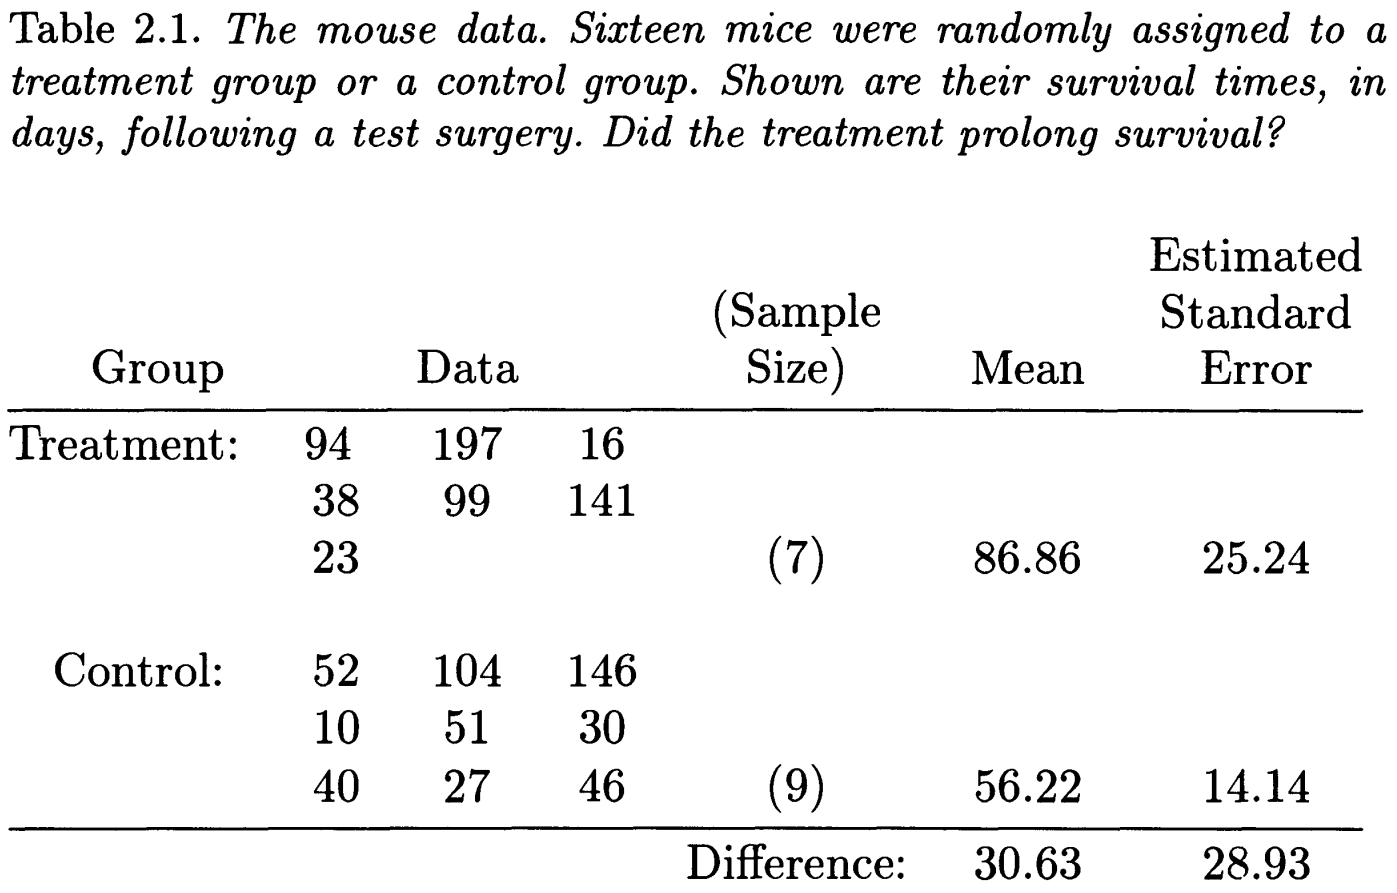
\includegraphics[width=\linewidth]{1/t1.png}
\newline

Продлило ли лечение выживаемость? Сравнение средних значений для двух групп дает предварительные основания для положительного ответа. Обозначим через $x_1,x_2,\ldots x_7$ продолжительность жизни в группе с лечением, соотв. $x_1=94,x_2=197,\ldots,x_7=23$, а через $y_1,y_2,\ldots y_9$ продолжительность жизни в контрольной группе. Групповые выборочные средние равны
\begin{equation}
    \overline x = \sum_{i=1}^7 x_i/7 = 86.86 \quad \texttt{и} \quad \overline y = \sum_{i=1}^9 y_i/9 = 56.22,
\end{equation}
таким образом разность $\overline x - \overline y$ равна $30.63$, что предполагает значительный эффект продления жизни при лечении.

Но насколько точны эти оценки? В конце концов, средние (2.1) основаны на небольших выборках, всего 7 и 9 мышей соответственно. Чтобы ответить на этот вопрос, нам нужна оценка точности выборочных средних $\overline x$ и $\overline y$). Для выборочных средних и по существу только для выборочных средних формулу точности получить легко. 

Расчетная стандартная ошибка среднего $\overline x$ на основе $n$ независимых наблюдений $x_1, x_2,\ldots, x_n$, $\overline x =\sum_{i=1}^n x_i/n$, определяется формулой 
\begin{equation}
    \sqrt{\frac{s^2}{n}},
\end{equation}
где $s^2=\sum_{i=1}^n (x_i-\overline x)^2/(n-1)$. (Эта формула и стандартные ошибки в целом обсуждаются более подробно в главе 4.) Стандартная ошибка любой оценки определяется как квадратный корень из ее дисперсии, то есть среднеквадратичная изменчивость оценки вокруг ее математического ожидания. Это наиболее распространенная мера точности оценок. Грубо говоря, оценка отличается от своего истинного значения менее чем на одну стандартную ошибку примерно в 68\% случаев и менее чем на две стандартные ошибки примерно в 95\% случаев.

Если бы оценочные стандартные ошибки в эксперименте на мышах были очень малы, скажем, менее 1, тогда мы бы знали, что $\overline x$ и $\overline y$ были близки к их истинным значениям и что наблюдаемая разница в 30,63, вероятно, была хорошей оценкой истинного увеличения выживаемости при лечении. С другой стороны, если формула (2.2) дает большие оценочные стандартные ошибки, скажем 50, тогда оценка разности будет слишком неточной, чтобы на нее можно было полагаться. 

Фактическая ситуация показана справа в Таблице 2.1. Расчетные стандартные ошибки, рассчитанные по (2.2), составляют 25,24 для $\overline x$ и 14,14 для $\overline y$. Стандартная ошибка для разности $\overline x - \overline y$ равна $28,93 = \sqrt{25,24^2 + 14,14^2}$ (поскольку дисперсия разности двух независимых величин является суммой их дисперсий). Мы видим, что наблюдаемая разница 30,63 составляет всего $30,63 / 28,93 = 1,05$ стандартной ошибки разности. Читатели, знакомые с теорией проверки гипотез, сочтут это незначимым результатом, который может легко возникнуть случайно, даже если лечение действительно не имело никакого эффекта. 

Обычно стандартные ошибки являются отличным первым шагом к критическому осмыслению статистических оценок. К сожалению, стандартные ошибки имеют серьезный недостаток: для большинства статистических оценок, отличных от среднего, не существует формулы, подобной (2.2), для получения стандартных ошибок. Другими словами, трудно оценить точность оценки, отличной от оценки среднего.

Предположим, например, что мы хотим сравнить две группы в таблице 2.1 по их медианам, а не по их средним значениям. Медианы составляют 94 для лечения и 46 для контроля, что дает разницу в 48, что значительно больше, чем разница средних значений. Но насколько точны эти медианы? Ответы на такие вопросы - вот где вступают в игру бутстреп и другие компьютерные методы. В оставшейся части этой главы дается краткий обзор начальной оценки стандартной ошибки - метода, который будет полностью обсуждаться в следующих главах. 

Предположим, что мы наблюдаем независимые данные $x_1, x_2,\ldots, x_n$, для удобства обозначенные вектором $X = (x_1, x_2, \ldots, x_n)$, по которым мы вычисляем интересующую статистику $s(X)$. Например, данные могут быть наблюдениями контрольной группы $n = 9$ в таблице 2.1, а $s(X)$ может быть средним по выборке. 

Бутстреп оценка стандартной ошибки, изобретенная Эфроном в 1979 году, выглядит совершенно иначе, чем (2.2), но на самом деле они тесно связаны. Бутстреп выборка $X^* = (x^*_i, x^*_2,\ldots, x^*_n)$ получается путем случайного выбора с возвращением $n$ точек из исходных данных $x_1, x_2,\ldots, x_n$. Например, при $n = 7$ мы можем получить $X^* = (x_5, x_7, x_5, x_4, x_7, x_3, x_1)$· 
\newline

\noindent
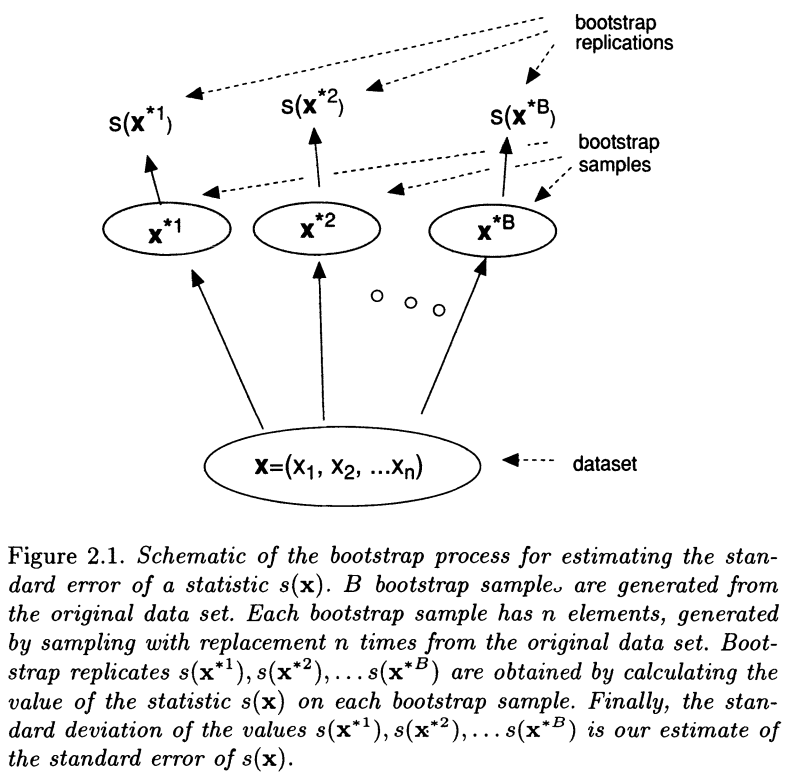
\includegraphics[width=\linewidth]{1/f1.png}
\newline

Рисунок 2.1 представляет собой схему процесса бутстрепа. Алгоритм бутстрепа начинается с генерации большого количества независимых бутстреп выборок $X^{*1}, X^{* 2},\ldots, X^{*B}$, каждая размером n. Типичные значения для B, количества бутстреп выборок, находятся в диапазоне от 50 до 200 для оценки стандартной ошибки. Каждой бутстреп выборке соответствует бутстреп репликация $s (X^{* b})$, посчитанная для $X^{* b}$. Если $s(X)$ - это, например, медиана выборки, то $s (X^*)$ - это медиана бутстреп выборки. Бутстреп оценка стандартной ошибки - это стандартное отклонение бутстреп репликаций  
\begin{equation}
    \hat{se}_{boot}=\left\{\sum_{b=1}^B [s(X^{*b})-s(\cdot)]^2/(B-1)\right\}^{\frac{1}{2}},
\end{equation}
где $s(\cdot)=\sum_{b=1}^B s(X^{*b})/B$. Предположим, что $s(X)=\overline X$. В этом случае стандартная теория вероятностей говорит нам, что, когда B становится очень большим, формула (2.3) приближается к  
\begin{equation}
    \left\{\sum_{i=1}^n (x_i-\overline x)^2/n^2\right\}^{\frac{1}{2}}.
\end{equation}

Это почти то же самое, что и формула (2.2). Мы могли бы сделать это точно таким же, умножив определение (2.3) на множитель $[n / (n-1)] ^\frac{1}{2}$, но в этом нет практического смысла. 
\newline

\noindent
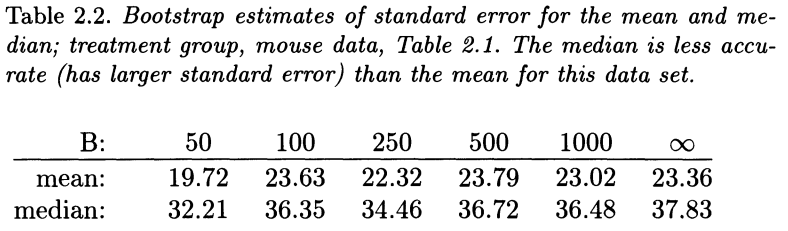
\includegraphics[width=\linewidth]{1/t2.png}
\newline

В таблице 2.2 показаны бутстрап оценки стандартной ошибки для среднего и медианы для данных экспериментальной группы мышей из таблицы 2.1. Стандартные ошибки уменьшаются до предельных значений по мере увеличения числа бутстраповых выборок $B$. Предельное значение $23,36$ для среднего получается из (2.4). Формула для предельного значения $37,83$ для стандартной ошибки медианы довольно сложна. 

Теперь мы можем оценить точность разницы медиан между двумя группами. Описанная выше бутстреп процедура, примененная к контрольной группе, дала оценку стандартной ошибки $11,54$ на основе $B = 100$ повторений ($B = \infty$ дало $9,73$). Следовательно, используя $B = 100$, наблюдаемая разница в $48$ имеет расчетную стандартную ошибку $\sqrt{36,35^2 + 11,54^2} = 38,14$, и, следовательно, $48 / 38,14 = 1,26$ стандартной ошибки. Это больше, чем наблюдаемая разница в средних, но все же незначимо. 

Для большинства статистических данных у нас нет формулы для предельного значения стандартной ошибки, но на самом деле формула не нужна. Вместо этого мы используем числовой вывод бутстреп программы для некоторого удобного значения B. Легко написать бутстреп программу, которая работает для любой вычислимой статистики $s (X)$. Имея эти программы, аналитик данных может свободно использовать любую статистику, независимо от ее сложности, с уверенностью, что он или она также будет иметь разумное представление о точности оценки. Применение бутстрепа стало доступным, поскольку компьютеры стали мощнее и дешевле. 
Стандартные ошибки - это простейшие меры статистической точности. В последующих главах показано, как бутстреп методы могут оценивать более сложные меры точности, такие как смещения, ошибки прогнозирования и доверительные интервалы. Бутстрепированные доверительные интервалы увеличивают вычислительную нагрузку еще в 10 раз. Результатом всех этих вычислений является увеличение количества статистических проблем, которые могут быть проанализированы, сокращение допущений анализа и устранение рутинных, но утомительных теоретических расчетов, обычно связанных с оценкой точности. 

\chapter{Случайные выборки и вероятности}
\section{Введение}

Статистика - это теория накопления информации, особенно информации, поступающей постепенно. Типичная статистическая ситуация была проиллюстрирована данными по мышам в Таблице 2.1. Ни одна мышь не предоставляет много информации, поскольку индивидуальные результаты очень различаются, но семь или девять мышей, взятых вместе, начинают быть весьма информативными. Статистическая теория касается лучших способов извлечения этой информации. Теория вероятностей обеспечивает математическую основу для статистических выводов. В этой главе рассматривается простейшая вероятностная модель, используемая для моделирования случайных данных: случай, когда наблюдения представляют собой случайную выборку из одной неизвестной совокупности, свойства которой мы пытаемся узнать из наблюдаемых данных. 
\section{Случайные выборки}

Проще всего визуализировать случайные выборки в терминах конечной совокупности или «вселенной» $\mathbf{U}$ отдельных единиц $U_1, U_2, \ldots, U_n$, любая из которых с равной вероятностью будет выбрана в одном случайном розыгрыше. В состав единиц могут входить все зарегистрированные избиратели в районе, подвергающемся политическому обследованию, все мужчины, которые предположительно могут быть выбраны для медицинского эксперимента, все средние школы в Соединенных Штатах и т.д. У отдельных единиц есть свойства, которые нам нужны. чтобы узнать, например, о политических взглядах, времени выживания в медицине или количестве выпускников. Слишком сложно и дорого исследовать каждую единицу в $\mathbf{U}$, поэтому мы выбираем для наблюдения случайную выборку управляемого размера. 

Случайная выборка размера $n$ определяется как набор из $n$ единиц $u_1, u_2,\ldots, u_n$, выбранных случайным образом из $\mathbf{U}$. В принципе, процесс выборки происходит следующим образом: устройство случайных чисел независимо выбирает целые числа $j_1 , j_2,\ldots, j_n$, каждое из которых равно любому значению от 1 до $N$ с вероятностью $1 / N$. Эти целые числа определяют, какие члены $\mathbf{U}$ выбраны для случайной выборки, $u_1 = U_{j_1}, u_2 = U_{j_2},\ldots,u_n=U_{j_n}$. На практике процесс отбора редко бывает таким аккуратным, и совокупность $\mathbf{U}$ может быть плохо определена, но концептуальная структура случайной выборки по-прежнему полезна для понимания статистических выводов. (Методология хорошего экспериментального дизайна, например, случайное распределение выбранных единиц в экспериментальную или контрольную группы, как это было сделано в эксперименте на мышах, помогает сделать теорию случайной выборки более применимой к реальным ситуациям, подобным той, что представлена в таблице 2.1.) 

Наше определение случайной выборки позволяет одной единице $U_i$ появляться в выборке более одного раза. Мы могли бы избежать этого, настаивая на том, чтобы целые числа $j_1, j_2,\ldots, j_n$ были различными, что называется <<выборкой без замены>>. Чуть проще разрешить повторы, то есть <<выборку с заменой>>, как в предыдущем абзаце. Если размер случайной выборки $n$ намного меньше, чем размер генеральной совокупности $N$, как это обычно бывает, вероятность повторения выборки в любом случае будет мала. См. Проблему 3.1. Случайная выборка всегда означает выборку с заменой в дальнейшем, если не указано иное. 

Выбрав случайную выборку $u_1, u_2,\ldots, u_n$, мы получаем одно или несколько представляющих интерес измерений для каждой единицы. Пусть $x_i$ обозначает измерения для единицы $u_i$. Наблюдаемые данные представляют собой набор измерений $x_1, x_2,\ldots, x_n$. Иногда мы будем обозначать наблюдаемые данные $(x_1, x_2, \ldots, x_n)$ одним символом $X$. 

Мы можем представить себе, как проводить измерения для каждого члена $U_1, U_2, \ldots ,U_N$ из $\mathbf{U}$, получая значения $X_1, X_2, \ldots, X_N$. Это можно было бы назвать переписью $U$. 

Символ $\mathbf{X}$ будет обозначать перепись измерений $(X_1, X_2,\ldots, X_N)$. Мы также будем называть $\mathbf{X}$ совокупностью измерений или просто совокупностью и называть $X$ случайной выборкой размера $n$ из $\mathbf{X}$. На самом деле мы обычно не можем позволить себе провести перепись, поэтому мы взяли случайную выборку. Цель статистического вывода -- сказать, что мы узнали о популяции $\mathbf{X}$ из наблюдаемых данных $X$. В частности, мы будем использовать бутстреп, чтобы сказать, насколько точно статистика, вычисленная из $x_1, x_2,\ldots, x_n$ (например, медиана выборки), оценивает соответствующее количество для всей генеральной совокупности. 
\newline

\noindent
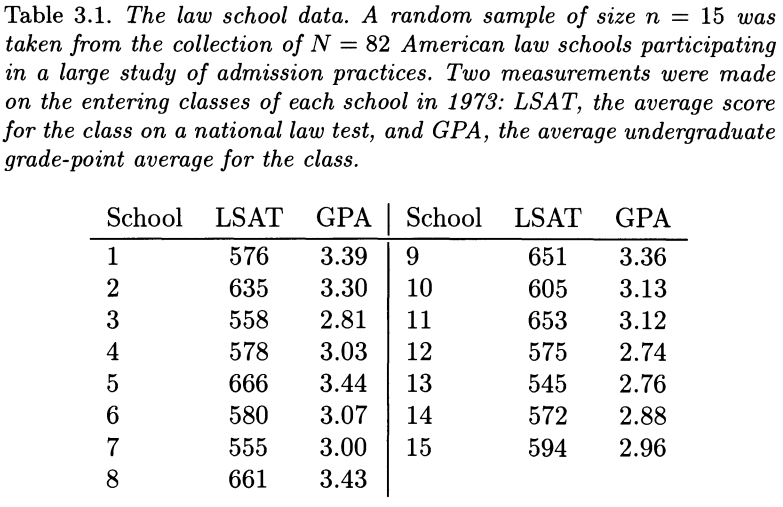
\includegraphics[width=\linewidth]{2/t21.png}
\newline

В таблице 3.1 показана случайная выборка размером $n = 15$, составленная из 82 американских юридических школ. Фактически показаны два измерения, проведенные для поступающих в 1973г. для каждого учебного заведения в выборке: LSAT, средний балл класса на экзамене по национальному праву, и GPA, средний балл бакалавриата, полученный студентами. В этом случае измерение $x_i$ на $u_i$, $i$-м члене выборки, представляет собой пару 
\begin{equation*}
    x_i=(LSAT_i, GPA_i)\quad i=1,2,\cdots,15
\end{equation*}
Наблюдаемые данные $x_1, x_2,\ldots, x_n$ представляют собой набор из 15 пар чисел, показанных в таблице 3.1. 

Этот пример является искусственным, потому что перепись данных $X_1, X_2,\cdots, X_82$ действительно была проведена. Другими словами, LSAT и GPA доступны для всей совокупности $N = 82$ школ. На Рисунке 3.1 показаны данные переписи и выборочные данные. В таблице 3.2 приведены все измерения $N$. 
\newline

\noindent
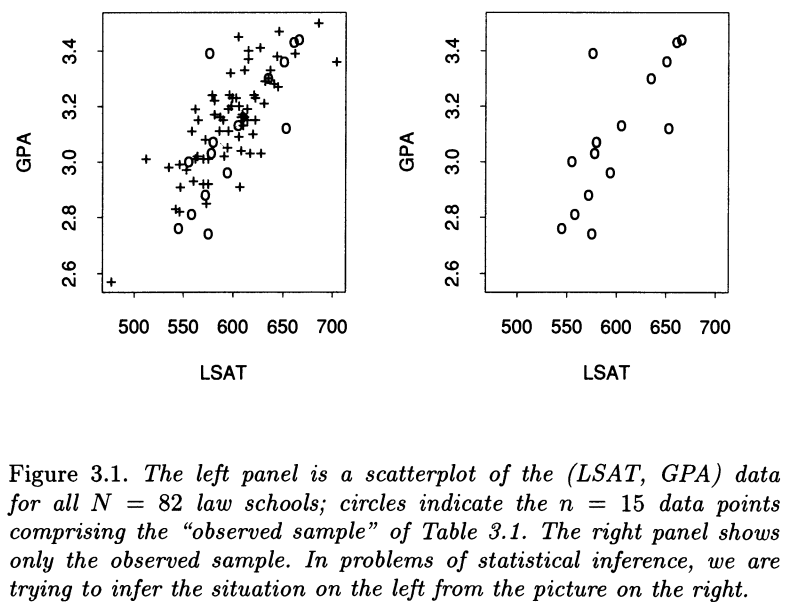
\includegraphics[width=\linewidth]{2/f31.png}
\newline

В реальной статистической задаче, такой как в таблице 3.1, мы увидим только выборочные данные, из которых мы попытаемся сделать вывод о свойствах совокупности. Например, рассмотрим 15 баллов LSAT в наблюдаемой выборке. Они имеют среднее значение $600.27$ с расчетной стандартной ошибкой $10.79$, основанной на данных в таблице 3.1 и формуле (2.2). Вероятность того, что истинное среднее значение LSAT, среднее для всей генеральной совокупности, из которой были взяты наблюдаемые данные, составляет около 68\%, находится в интервале $600.27 \pm 10.79$. 

Мы можем проверить этот результат, поскольку имеем дело с искусственным примером, для которого известны полные данные о населении. Среднее значение всех 82 значений LSAT составляет $597.55$, оно лежит в пределах прогнозируемого доверительного интервала $600.27 \pm 10.79$. 
\newline

\noindent
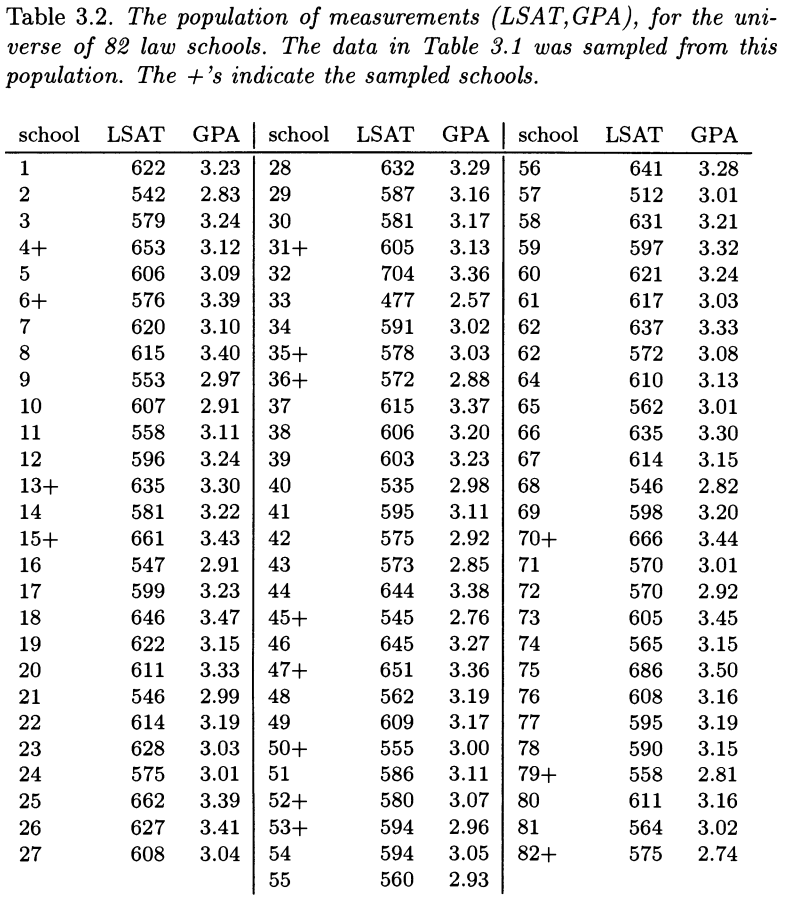
\includegraphics[width=\linewidth]{2/t32.png}
\newline
\section{Теория вероятностей}

Статистический вывод касается обучения на опыте: мы наблюдаем случайную выборку $\mathbf{x} = (x_1, x_2, \cdots, x_n)$ и хотим вывести свойства полной совокупности $\mathbf{X} = (X_1, X_2,\cdots, X_N)$, которая дала образец. Теория вероятностей идет в противоположном направлении: из состава популяции $\mathbf{X}$ мы выводим свойства случайной выборки $\mathbf{x}$ и статистики, вычисляемой по $\mathbf{x}$. Статистический вывод как математическая наука был разработан почти исключительно в терминах теории вероятностей. Здесь мы кратко рассмотрим некоторые фундаментальные концепции вероятности, включая распределения вероятностей, ожидания и независимость. 

В качестве первого примера пусть $x$ представляет результат броска правильной кости, поэтому $x$ с равной вероятностью будет 1, 2, 3, 4, 5 или 6. Мы запишем это в вероятностной нотации как 
\begin{equation}
    Prob\{x=k\}=1/6\qquad for\quad k=1,2,3,4,5,6.
\end{equation}

Случайное число, такое как $x$, часто называется случайной величиной. 

Вероятности - это идеализированные или теоретические пропорции. Мы можем представить себе пространство $\mathbf(U) = \{U_1 U_2, \cdots, U_N\}$ возможных бросков кубика, где $U_j$ полностью описывает физический акт j-го броска с соответствующими результатами $\mathbf{X} = (X_1, X_2,\cdots, X_N)$. Здесь $N$ может быть очень большим или даже бесконечным. Выражение $Prob\{x = 5\} = 1/6$ означает, что случайным образом выбранный член $\mathbf{X}$ имеет 1/6 шанс быть равным 5, или, проще говоря, 1/6 членов $\mathbf{X}$ равняется 5. Обратите внимание что такие вероятности, как пропорции, никогда не могут быть меньше 0 или больше 1. 

Для удобства обозначений определим частоты $f_k$, 
\begin{equation}
    f_k=Prob\{x=k\},
\end{equation}
так что у справедливой кости $f_k = 1/6$ для $k = 1, 2, \cdots, 6$. Распределение вероятностей случайной величины $x$, которую мы обозначим $F$, является любым полным описанием вероятностного поведения $x$. $F$ также называется распределением вероятностей популяции $\mathbf{X}$. Здесь мы можем взять $F$ как вектор частот 
\begin{equation}
    F=(f_1,f_2,\cdots,f_6)=(1/6, 1/6, \cdots,1/6).
\end{equation}
Несправедливым будет кубик, для которого $F$ не равно $(1/6, 1/6, \cdots,1/6)$. 

Некоторые распределения вероятностей возникают настолько часто, что получили специальные названия. Говорят, что случайная величина $x$ имеет биномиальное распределение с размером $n$ и вероятностью успеха $p$, что обозначается 
\begin{equation}
    x\sim Bi(n,p),
\end{equation}
если его частоты 
\begin{equation}
    f_k=C_n^kp^k(1-p)^{n-k}\quad for\quad k=0,1,2,\cdots,n.
\end{equation}
Здесь $n$ -- положительное целое число, $p$ -- число от 0 до 1, а $C_n^k$ -- биномиальный коэффициент $n! / [K! (n-k)!]$. На рисунке 3.2 показано распределение $F = (f_0, f_1, \cdots, f_n)$ для $x \sim Bi (n, p)$, при $n = 25$ и $p = 0.25, 0.50$ и $0.90$. Мы также пишем $F = Bi (n, p)$ для обозначения ситуации (3.4). 
\newline

\noindent
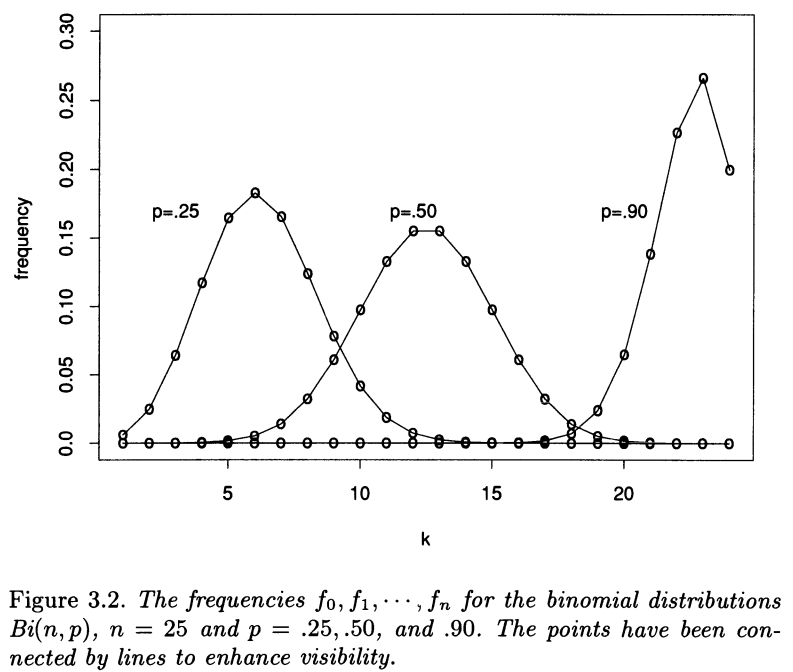
\includegraphics[width=\linewidth]{2/f32.png}
\newline

Пусть $A$ -- набор целых чисел. Тогда вероятность того, что $x$ принимает значение в $A$, или, проще говоря, вероятность $A$, равна 
\begin{equation}
    Prob\{x\in A\}=Prob\{A\}=\sum_{k\in A}f_k.
\end{equation}
Например, если $A = \{1, 3, 5, \cdots, 25\}$ и $x \sim Bi (25, p)$, то $Prob \{A\}$ -- это вероятность того, что биномиальная случайная величина размера 25 и вероятность успеха $p$ равно нечетному целому числу. Заметьте, что, поскольку $f_k$ -- это теоретическая доля раз, когда $x$ равно $k$, сумма $\sum_{k\in A}f_k = Prob \{A\}$ -- это теоретическая доля раз, когда $x$ принимает свое значение в $A$. 

Выборочное пространство $x$, обозначенное $S_x$, представляет собой набор возможных значений $x$. Для правильного кубика $S_x = \{1, 2, \cdots, 6\}$, а $S_x = \{0, 1, 2, \cdots, n\}$ для распределения $Bi (n, p)$. По определению $x$ встречается в $S_x$ каждый раз, то есть с теоретической пропорцией 1, поэтому
\begin{equation}
    Prob\{S_x\}=\sum_{k\in S_x}f_k=1.
\end{equation}
Для любого распределения вероятностей целых чисел частоты $f_j$ являются неотрицательными числами, сумма которых равна 1. 

В наших примерах до сих пор пространство выборки $S_x$ было подмножеством целых чисел. Одна из удобных особенностей вероятностных распределений заключается в том, что их можно определять в довольно общих пространствах. Рассмотрим данные юридического факультета на Рисунке 3.1. Мы могли бы принять $S_x$ за положительный квадрант плоскости
\begin{equation}
    S_x=\mathbf{R}^{2+}=\{(y,z),y>0,z>0\}.
\end{equation}
(Сюда входят такие значения, как $x = (10^6, 10^9)$, но не повредит, если $S_x$ будет слишком большим.) Для подмножества $A$ из $S_x$ мы все равно будем писать $Prob \{A\}$, чтобы указать вероятность того, что $x$ встречается в $A$. 

Например, мы могли бы взять 
\begin{equation}
    A=\{(y,z):0<y<600,0<z<3.0\}.
\end{equation}
Юридическая школа $x \in A$, если ее входной класс 1973 года имел LSAT менее 600 и средний балл менее 3,0. В этом случае мы знаем полную популяцию $\mathbf{X}$; это 82 точки, указанные на левой панели рисунка 3.1 и в таблице 3.2. Из них 16 находятся в $A$, поэтому 
\begin{equation}
    Prob\{A\}=16/82=0.195.
\end{equation}
Здесь идеализированная пропорция $Prob \{A\}$ -- это действительная пропорция. Только в тех случаях, когда у нас есть полная генеральная совокупность, можно напрямую оценить вероятности как пропорции. 

Распределение вероятностей $F$ $x$ по-прежнему определяется как полное описание вероятностей $x$. В примере с юридической школой $F$ можно описать следующим образом: для любого подмножества $A$ из $S_x = \mathbf{R}^{2+}$, 
\begin{equation}
    Prob\{x\in A\}=\#\{X_j\in A\}/82,
\end{equation}
где $\# \{X_j \in A\}$ -- это 82 точки на левой панели рисунка 3.1, которые лежат в $A$. Другим способом сказать, что $F$ -- это дискретное распределение, полагая вероятность (или частоту) 1/82 на каждую из указанных 82 точек. 

Вероятности можно определять непрерывно, а не дискретно, как в (3.6) или (3.11). Самый известный пример -- нормальное (или гауссово, или колоколообразное) распределение. Определено, что случайная величина $x$ с действительными значениями имеет нормальное распределение со средним $\mu$ и дисперсией $\sigma^2$, записанное 
\begin{equation}
    x\sim N(\mu,\sigma^2)\quad or \quad F=N(\mu,\sigma^2),
\end{equation}
если
\begin{equation}
    Prob\{x\in A\}=\int_A\frac{1}{\sqrt{2\pi\sigma^2}}\exp^{-\frac{1}{2}(\frac{x-\mu}{\sigma})^2}dx
\end{equation}
для любого подмножества $A$ действительной прямой $\mathbf{R}^1$. Интеграл в (3.13) берется по значениям $x \in A$. 

Существуют версии нормального распределения с более высокой размерностью, которые включают взятие интегралов, подобных (3.13), по многомерным множествам $A$. Нам не понадобятся непрерывные распределения для разработки бутстрепа. Как мы увидим, одним из основных стимулов для развития бутстрепа является желание заменить теоретические вычисления компьютерными с использованием специальных распределений. 

Математическое ожидание вещественной случайной величины $x$, обозначаемой $E(x)$, является ее средним значением, где среднее значение берется по возможным результатам $x$, взвешенным в соответствии с его распределением вероятностей $F$. Таким образом, 
\begin{equation}
    E(x)=\sum_{x=0}^nxC_n^xp^x(1-p)^x\quad for\quad x\sim Bi(n,p),
\end{equation}
и
\begin{equation}
    E(x)=\int_{-\infty}^\infty x\frac{1}{\sqrt{2\pi\sigma^2}}\exp^{-\frac{1}{2}(\frac{x-\mu}{\sigma})^2}dx\quad for \quad x\sim N(\mu,\sigma^2).
\end{equation}
Нетрудно показать, что $E(x) = np$ для $x \sim Bi (n, p)$ и $E (x) = \mu$ для $x \sim N (\mu, \sigma^2)$.

Иногда мы пишем математическое ожидание как $E_F (x)$, чтобы указать, что среднее значение берется по отношению к распределению $F$.

Предположим, что $r = g (x)$ -- некоторая функция случайной величины $x$. Тогда $E (r)$, математическое ожидание $r$, представляет собой теоретическое среднее значение $g (x)$, взвешенное в соответствии с распределением вероятности $x$. Например, если $x \sim  N (\mu, \sigma^2)$ и $r = x^3$, то 
\begin{equation}
    E(r)=\int_{-\infty}^\infty x^3\frac{1}{\sqrt{2\pi\sigma^2}}\exp^{-\frac{1}{2}(\frac{x-\mu}{\sigma})^2}dx.
\end{equation}

Вероятности -- это частный случай ожиданий. Пусть $A$ -- подмножество $S_x$, и возьмем $r = I_{\{x\in A\}}$, где $I_{\{x\in A\}}$ - индикаторная функция
\begin{equation}
    I_{\{x\in A\}}=\begin{cases}
      1\quad if \quad x\in A\\
      0\quad if \quad x\not\in A
    \end{cases}.
\end{equation}
Тогда $E(r)$ равна $Prob\{x\in A\}$ или 
\begin{equation}
    E(I_{\{x\in A\}})=Prob\{x\in A\}.
\end{equation}
Например, если $x\sim N(\mu, \sigma^2)$, тогда
\begin{equation}
    E(r)=\int_{-\infty}^\infty I_{\{x\in A\}}\frac{1}{\sqrt{2\pi\sigma^2}}\exp^{-\frac{1}{2}(\frac{x-\mu}{\sigma})^2}dx=
    \int_{A} \frac{1}{\sqrt{2\pi\sigma^2}}\exp^{-\frac{1}{2}(\frac{x-\mu}{\sigma})^2}dx,
\end{equation}
является $Prob\{x\in A\}$ в соответствии с (3.13).

Понятие математического ожидания как теоретического среднего является очень общим и включает случаи, когда случайная величина $x$ не является действительной. В ситуации с юридической школой, например, нас может заинтересовать математическое ожидание соотношения LSAT и GPA. Пусть $x = (y, z)$, как в (3.8), тогда $r = y/z$, и математическое ожидание $r$ равно 
\begin{equation}
    E(LSAT/GPA)=\frac{1}{82}\sum_{j=1}^82(y_j/z_j)
\end{equation}
где $x_j = (y_j, z_j)$ -- j-я точка в таблице 3.2. Численная оценка (3.20) дает $E(LSAT/GPA) = 190.8$. 

Пусть $\mu_x = E_F(x)$ для $x$ вещественной случайной величины с распределением $F$. Дисперсия $x$, обозначаемая $\sigma^2_x$ или просто $\sigma^2$, определяется как ожидаемое значение $y = (x- \mu)^2$. Другими словами, $\sigma^2$ -- это теоретический средний квадрат расстояния случайной величины $x$ от ее математического ожидания $\mu$, 
\begin{equation}
    \sigma^2_x = E_F(x-\mu_x)^2.
\end{equation}
Дисперсия $x\sim N (\mu, \sigma^2)$ равна $\sigma^2$; дисперсия $x\sim Bi (n, p)$ равна $np (1 - p)$. Стандартное отклонение случайной величины определяется как квадратный корень из ее дисперсии. 

Две случайные величины $y$ и $z$ называются независимыми, если 
\begin{equation}
    E[g(y)h(z)]=E[g(y)]E[h(z)]
\end{equation}
для всех функций $g(y)$ и $h(z)$. Независимость (3.22) подразумевает, что случайный результат $y$ не влияет на случайный результат $z$, и наоборот. 

Чтобы убедиться в этом, пусть $B$ и $C$ - подмножества $S_y$ и $S_z$ соответственно, выборочные пространства $y$ и $z$, а $g$ и $h$ - индикаторные функции $g(y) = I_{\{y\in B\}}$ и $h (z) = I_{\{z\in C\}}$ · Обратите внимание, что 
\begin{equation}
    I_{\{y\in B\}}I_{\{z\in C\}}=\begin{cases}
      1\quad if \quad y\in B\quad and\quad z\in C\\
      0\quad otherwise.
    \end{cases}
\end{equation}
Итак, $I_{\{y\in B\}}I_{\{z\in C}\}$ -- индикаторная функция пересечения ${\{y \in B\}} \cap {\{z \in C\}}$. Тогда в силу (3.18) и определения независимости (3.22) 
\begin{equation}
    \begin{array}{l}
        Prob\{(y,z)\in B\cap C\} = E(I_{\{y\in B\}}I_{\{z\in C\}})=\\ \\
        =E(I_{\{y\in B\}})E(I_{\{z\in C\}}) = Prob\{y\in B\}Prob\{z\in C\}.
    \end{array}
\end{equation}

Глядя на рисунок 3.1, мы видим, что (3.24) не выполняется для примера юридической школы, поэтому LSAT и GPA не являются независимыми. 

Независимо от того, независимы ли $y$ и $z$, ожидания подчиняются простому правилу сложения 
\begin{equation}
    E[g(y)+h(z)]=E[g(y)]+E[h(z)].
\end{equation}
В общем виде
\begin{equation}
    E[\sum_{i=1}^ng_i(x_i)]=\sum_{i=1}^nE[g_i(x_i)]
\end{equation}
для любых функций $g_i$ и любых $n$ случайных величин $x_1, x_2,\cdots, x_n$. 

Случайная выборка с заменой гарантирует независимость: если $x = (x_1, x_2,\cdots, x_n)$ -- случайная выборка размера $n$ из совокупности $\mathbf{X}$, то все $n$ наблюдений $x_i$ одинаково распределены и взаимно независимы друг от друга. Другими словами, все $x_i$ имеют одинаковое распределение вероятностей $F$, и 
\begin{equation}
    E_F[g_1(x_1)g_2(x_2)\cdots g_n(x_n)] = E_F[g_1(x_1)]E_F[g_2(x_2)]\cdots E_F[g_n(x_n)] 
\end{equation}
для любых функций $g_1,g_2,\cdots, g_n$. (Это почти определение того, что означает случайная выборка.) Будем пиcать 
\begin{equation}
    F\rightarrow (x_1,x_2,\cdots,x_n)
\end{equation}
чтобы указать, что $x = (x_1, x_2, \cdots, x_n)$ является случайной выборкой размера $n$ из совокупности с распределением вероятностей $F$. Иногда это записывается как 
\begin{equation}
    x\iid F\qquad i=1,2,\cdots,n,
\end{equation}
где i.i.d. означает независимый и одинаково распределенный.

\chapter{Эмпирическая функция распределения и принцип плагина}
\section{Введение}

Проблемы статистического вывода часто включают оценку некоторого свойства распределения вероятностей $F$ на основе случайной выборки, взятой из $F$. Эмпирическая функция распределения, которую мы будем называть $\hat F$, представляет собой простую оценку всего распределения $F$. Оценка какого-то интересующего свойства $F$, например его среднего значения, медианы или корреляции, заключается в использовании соответствующего свойства $\hat F$. Это «принцип плагина». Как мы увидим в главе 6, метод бутстрепа является прямым применением принципа плагина. 
\section{Эмпирическая функция распределения}

Пусть дана случайная выборка размера $n$ из распределения вероятностей $F$
\begin{equation}
    F\rightarrow(x_1,x_2,\cdots,x_n),
\end{equation}
тогда эмпирическая функция распределения  $F$ определяется как дискретное распределение, которое ставит вероятность $1 / n$ на каждое значение $x_i$, $i = 1, 2, \cdots, n$. Другими словами, $F$ присваивает множеству $A$ в пространстве выборок $x$ его эмпирическую вероятность 
\begin{equation}
    \widehat{Prob}\{A\}=\#\{x_i\in A\}/n,
\end{equation}
это доля наблюдаемой выборки $x = (x_1, x_2,\cdots, x_n)$, встречающейся в A. Мы также будем писать $Prob_{\hat F}\{A\}$ для обозначения (4.2). Символ в шляпе <<$\wedge$>> всегда указывает на величины, рассчитанные на основе наблюдаемых данных. 
\newline

\noindent
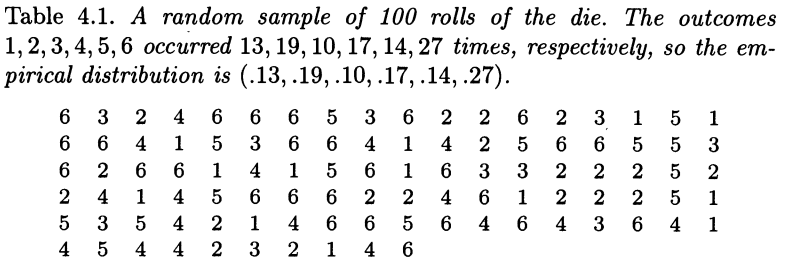
\includegraphics[width=\linewidth]{3/t41.png}
\newline

Рассмотрим выборку юридических вузов размером $n = 15$, показанную в Таблице 3.1 и на правой панели Рисунка 3.1. Эмпирическое распределение $F$ ставит вероятность $1/15$ для каждой из 15 точек данных. Пять из 15 точек лежат в наборе $A = \{(y, z): 0 <y <600,0 <z <3.00\}$, поэтому $\widehat{Prob}\{A\} = 5/15 = 0.333$. Обратите внимание, что мы получаем другую эмпирическую вероятность для набора $\{0 <y <600,0 <z \le 3.00\}$, поскольку одна из 15 точек данных имеет $GPA = 3.00$, $LSAT < 600$. 

Таблица 4.1 показывает случайную выборку из $n = 100$ бросков кубика: $x_1 = 6, x_2 = 3, x_3 = 2,\cdots, x_{100} = 6$. Эмпирическое распределение $F$ ставит вероятность $1/100$ для каждого из 100 исходов. В подобных случаях, когда есть повторяющиеся значения, мы можем более экономично выразить $F$ как вектор наблюдаемых частот $\hat f_k$, $k=1,2,\cdots,6$
\begin{equation}
    \hat f_k = \#\{x_i=k\}/n.
\end{equation}
Для данных в таблице 4.1 $\hat F= (0.13, 0.19, 0.10, 0.17, 0.14, 0.27)$.

Эмпирическое распределение -- это список значений, принимаемых выборкой $x = (x_1, x_2, \cdots, x_n)$, вместе с долей случаев, когда каждое значение встречается. Часто каждое значение, встречающееся в выборке, появляется только один раз, как в случае с данными юридических школ. Повторения, как и в случае с кубиком таблицы 4.1, позволяют сократить список. В любом случае каждой из $n$ точек данных $x_i$ приписывается вероятность $1 / n$ эмпирическим распределением. 

Очевидно ли, что мы не потеряли информацию при переходе от полного набора данных $(x_1, x_2,\cdots, x_{100})$ в таблице 4.1 к сокращенному представлению в терминах частот? Нет, но это правда. Можно доказать, что вектор наблюдаемых частот $\hat F = (\hat f_1, \hat f_2, \cdots)$ является достаточной статистикой для истинного распределения $F = (f_1, f_2, \cdots)$. Это означает, что вся информация о $F$, содержащаяся в $\mathbf{x}$, также содержится в $\hat F$. 
\newline

\noindent
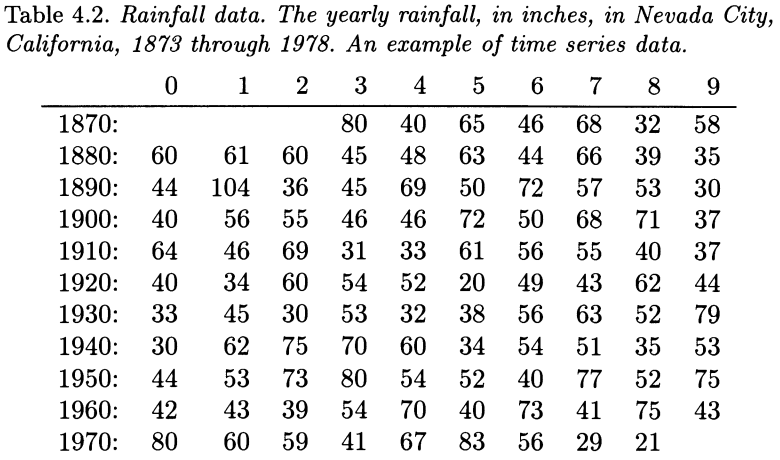
\includegraphics[width=\linewidth]{3/t42.png}
\newline

Теорема достаточности предполагает, что данные были сгенерированы случайной выборкой из некоторого распределения $F$. Это, конечно, не всегда верно. Например, данные о мышах в Таблице 2.1 включают два распределения вероятностей, одно для лечения и одно для контроля. В таблице 4.2 показан временной ряд из 106 чисел: годовое количество осадков в Невада-Сити, Калифорния, с 1873 по 1978 год. Мы могли бы вычислить эмпирическое распределение $F$ для этого набора данных, но оно не будет включать никакой информации временного ряда, например, если большие числа следуют за большими числами. На данный момент мы ограничиваем внимание данными, полученными путем случайной выборки из одного распределения, так называемой ситуации с одной выборкой. Это не так строго, как кажется. Например, в примере с данными о мышах мы можем применить результаты по одной выборке отдельно к экспериментальной и контрольной популяциям. 

При применении статистической теории к реальным задачам ответы на интересующие вопросы обычно формулируются в терминах вероятностных распределений. Мы можем спросить, справедлива ли матрица, дающая данные в Таблице 4.1. Это эквивалентно вопросу, равно ли распределение вероятностей $F$ кубика $(1/6, 1/6, 1/6, 1/6, 1/6, 1/6)$. В примере с юридической школой вопрос может заключаться в том, насколько коррелируют LSAT и GPA. В терминах $F$, распределение $x = (y, z) = (LSAT, GPA)$, это вопрос о значении коэффициента корреляции совокупности
\begin{equation}
    corr(y,z)=\frac{\sum_{j=1}^{82}(Y_j-\mu_y)(Z_j-\mu_z)}{[\sum_{j=1}^{82}(Y_j-\mu_y)^2\sum_{j=1}^{82}(Z_j-\mu_z)^2]^\frac{1}{2}},
\end{equation}
где $(Y_j, Z_j)$ -- j-я точка в популяции юридических школ $\mathbf{X}$, а $\mu_y = \sum_{j=1}^{82} Y_j / 82$, $\mu_z = \sum_{j=1}^{82} Z_j / 82$.

Когда распределение вероятностей $F$ известно (т.е. когда у нас есть полная совокупность $\mathbf{X}$), ответы на такие вопросы требуют не более чем арифметических операций. Для совокупности юридических школ перепись в таблице 3.2 дает $\mu_y = 597.5$, $\mu_z = 3.13$ и 
\begin{equation}
    corr(y,z)=0.761.
\end{equation}
Это первоначальное определение «статистики». Обычно у нас нет генеральной совокупности. Поэтому нам нужен статистический вывод, более современная статистическая теория для вывода свойств $F$ из случайной выборки $\mathbf{x}$. 

Если бы у нас была только выборка юридических школ размером 15, таблица 3.1, мы могли бы оценить $corr (y, z)$ с помощью коэффициента корреляции выборки 
\begin{equation}
    \widehat{corr}(y,z)=\frac{\sum_{j=1}^{15}(y_j-\hat\mu_y)(z_j-\hat\mu_z)}{[\sum_{j=1}^{15}(y_j-\hat\mu_y)^2\sum_{j=1}^{15}(z_j-\hat\mu_z)^2]^\frac{1}{2}},
\end{equation}
где $(y_j, z_j)$ - j-я точка в таблице 3.1, $j = 1, 2, \cdots, 15$ и $\hat\mu_y = \sum_{j=1}^{15}y_j/15$, $\hat\mu_z = \sum_{j=1}^{15}z_j / 15$. Таблица 3.1 дает $\mu_y = 600.3$, $\mu_z = 3.09$ и 
\begin{equation}
    \widehat{corr}(y,z)=0.776.
\end{equation}

Вот еще один пример оценки плагина. Предположим, нас интересует оценка вероятности того, что результат LSAT превышает 600, то есть 
\begin{equation}
    \theta=\frac{1}{82}\sum_1^{82}I_{\{Y_i>600\}}.
\end{equation}
Поскольку 39 из 82 баллов LSAT превышают 600, $\theta = 39/82 = 0.48$. Плагин оценка $\theta$ доли баллов LSAT, превышающих 600, равна 
\begin{equation}
    \hat\theta=\frac{1}{15}\sum_1^{15}I_{\{y_i>600\}}.
\end{equation}
Шесть из 15 баллов LSAT превышают 600, поэтому $\hat\theta = 6/15 = 0.4$. 

Для кубика в Таблице 4.1 у нас нет данных переписи, а есть только выборка $\mathbf{x}$, поэтому на любые вопросы о справедливости кубика необходимо отвечать, исходя из эмпирических частот
\begin{equation}
    \hat F=(\hat f_1, \hat f_2,\cdots,\hat f_6)=(0.13,0.19,0.10,0.17,0.14,0.27).
\end{equation}

Обсуждения статистического вывода сформулированы в терминах параметров и статистики. Параметр -- это функция распределения вероятностей $F$. Статистика -- это функция выборки $\mathbf{x}$. Таким образом, $corr (y, z)$, (4.4), является параметром $F$, а $\widehat{corr} (y, z)$, (4.6), является статистикой, основанной на $\mathbf{x}$. Точно так же $f_k$ -- это параметр $F$, а $\hat f_k$ -- статистика, $k = 1, 2, 3, \cdots, 6$.

Иногда мы будем писать параметры напрямую как функции от $F$, например
\begin{equation}
    \theta=t(F).
\end{equation}
Это обозначение подчеркивает, что значение параметра $\theta$ получается путем применения некоторой процедуры численной оценки $t(\cdot)$ к функции распределения $F$. Например, если $F$ -- это распределение вероятностей на действительной прямой, математическое ожидание можно представить как параметр 
\begin{equation}
    \theta=t(F)=E_F(x).
\end{equation}
Здесь $t(F)$ или $\theta$ вычисляется через математическое ожидание, то есть среднее значение $x$, взвешенное в соответствии с $F$. Для распределения $F$, такого как $F = Bi (n, p)$, мы можем вычислить $t (F) = np$. Даже если $F$ неизвестна, форма $t (F)$ сообщает нам функциональное отображение из $F$ в $\theta$. 
\section{Принцип плагина}

Принцип плагина представляет собой простой метод оценки параметров по выборкам. Плагин оценка параметра $\theta = t (F)$ определяется как 
\begin{equation}
    \hat\theta=t(\hat F).
\end{equation}
Другими словами, мы оцениваем функцию $\theta = t (F)$ распределения вероятностей $F$ той же функцией эмпирического распределения $\hat F$, $\hat\theta = t (\hat F)$. (Статистические данные, подобные (4.13), которые используются для оценки параметров, иногда называют суммарной статистикой, а также оценками и оценщиками.) 

Мы уже использовали принцип плагина при оценке $f_k$ через $\hat f_k$ и при оценке $corr (y, z)$ с помощью $\widehat{corr} (y, z)$. Чтобы убедиться в этом, обратите внимание, что наша совокупность $F$ юридических школ может быть записана как $F = (f_1, f_2,\cdots ,f_82)$, где каждое $f_j$, вероятность j-го юридической школы, имеет значение 1/82. Это распределение вероятностей на $\mathbf{X}$, 82 парах юридических школ. Коэффициент корреляции генеральной совокупности можно записать как 
\begin{equation}
    corr(y,z)=\frac{\sum_{j=1}^{82}f_j(Y_j-\mu_y)(Z_j-\mu_z)}{[\sum_{j=1}^{82}f_j(Y_j-\mu_y)^2\sum_{j=1}^{82}f_j(Z_j-\mu_z)^2]^\frac{1}{2}},
\end{equation}
где
\begin{equation}
    \mu_y=\sum_{j=1}^{82}f_jY_j,\qquad\mu_z=\sum_{j=1}^{82}f_jZ_j.
\end{equation}
Установка каждого $f_j = 1/82$ дает выражение (4.4). Теперь для нашей выборки $(x_1, x_2,\cdots, x_15)$ выборочная частота $\hat f_j$ -- это доля точек выборки, равная $X_j$:
\begin{equation}
    \hat f_j=\#\{x_i=X_j\}/15, j=1,2,\ldots,82.
\end{equation}
Для выборки из Таблицы 3.1 $\hat f_1 = 0, \hat f_2 = 0, \hat f_3 = 0, \hat f_4 = 1/15$ и т.д. Теперь подставив эти значения $\hat f_j$ в выражения (4.15) и (4.14), получим $\hat\mu_y$, $\hat\mu_z$ и $\widehat{corr} (y, z)$ соответственно. То есть $\hat\mu_y$, $\hat\mu_z$ и $\widehat{corr} (y, z)$ -- это плагин оценки $\mu_y$, $\mu_z$ и $corr (y, z)$. 

В общем, плагин оценка математического ожидания $\theta = E_F (x)$ равна 
\begin{equation}
    \hat\theta = E_{\hat F} (x)=\frac{1}{n}\sum_{i=1}^nx_i=\bar x.
\end{equation}

Насколько хорош принцип плагина? Обычно, если единственная доступная информация о $F$ исходит из выборки $\mathbf{x}$, то $\hat\theta = t (\hat F)$ не может быть улучшена как оценка $\theta = t (F)$, по крайней мере, не в обычном асимптотическом ($n\rightarrow\infty$) смысле статистической теории. Например, если $\hat f_k$ -- плагин оценка частоты $\#\{x_i = k\} / n$, то 
\begin{equation}
    \hat f_k\sim Bi(n,f_k)/n.
\end{equation}
В этом случае оценка $\hat f_k$ является несмещенной для $f_k$, $E(\hat f_k) = f_k$, с дисперсией $f_k (1-f_k) / n$. Это наименьшая возможная дисперсия для несмещенной оценки $f_k$. 

Мы будем использовать бутстреп для изучения смещения и стандартной ошибки плагин оценки $\hat\theta = t (\hat F)$. Достоинство бутстрепа состоит в том, что он автоматически создает смещения и стандартные ошибки, независимо от того, насколько сложным может быть функциональное сопоставление $\theta = t (F)$. Мы увидим, что сам бутстреп является применением плагин принципа. 

Принцип плагина менее эффективен в ситуациях, когда имеется информация о $F$, отличная от той, которая предоставлена выборкой $\mathbf{x}$. Мы можем знать или предполагать, что $F$ является членом параметрического семейства, например семейства многомерных нормальных распределений. Или мы можем оказаться в ситуации регрессии, когда у нас есть набор случайных выборок $\mathbf{x} (z)$ в зависимости от переменной-предиктора $z$. Тогда, даже если нас интересует только $F_{z_0}$, функция распределения для некоторого конкретного значения $z_o$ из $z$, может быть информация о $F_{z_o}$ в других выборках $\mathbf{x} (z)$, особенно тех, для которых $z$ близок к $z_0$.

Принцип плагина и бутстреп могут быть адаптированы к параметрическим семействам и регрессионным моделям. В следующих нескольких главах мы предполагаем, что находимся в ситуации, когда у нас есть только одна случайная выборка $\mathbf{x}$ из полностью неизвестного распределения $F$. Это называется непараметрической задачей с одной выборкой.

\chapter{Стандартные ошибки и оценки стандартных ошибок}
\section{Введение}

Сводная статистика, такая как $\hat\theta = t (\hat F)$, часто является первым результатом анализа данных. Следующее, что мы хотим знать -- это точность $\hat\theta$. Бутстреп обеспечивает оценки точности, используя принцип плагина для оценки стандартной ошибки сводной статистики. Это предмет следующей главы. Сначала мы обсудим оценку стандартной ошибки среднего, где принцип плагина может быть реализован явно. 
\section{Стандартная ошибка среднего}

Предположим, что $x$ -- вещественная случайная величина с распределением вероятностей $F$. Обозначим математическое ожидание и дисперсию $F$ символами $\mu_F$ и $\sigma^2_F$ соответственно,
\begin{equation}
    \mu_F=E_F(x),\qquad \sigma^2_F=var_F(x)=E_F[(x-\mu_F)^2].
\end{equation}
В главе 3 эти величины назывались $\mu_x$ и $\sigma^2_x$. Здесь мы подчеркиваем зависимость от $F$. Альтернативное обозначение $var_F (x)$ для дисперсии, иногда сокращенное до $var (x)$, означает то же самое, что и $\sigma^2_F$. В дальнейшем мы иногда будем писать
\begin{equation}
    x\sim(\mu_F,\sigma^2_F)
\end{equation}
чтобы кратко обозначить математическоу ожидание и дисперсию $x$.

Теперь пусть $(x_1,\cdots, x_n)$ будет случайной выборкой размера $n$ из распределения $F$. Среднее значение выборки $\bar x = \sum_{i=1}^n x_i / n$ имеет математическое ожидание $\mu_F$ и дисперсию $\sigma^2_F/n$, 
\begin{equation}
    \bar x\sim(\mu_F,\sigma^2_F/n).
\end{equation}
Другими словами, математическоу ожидание $\bar x$ такое же, как ожидание одного $x$, но дисперсия $\bar x$ равна $1 / n$ дисперсии $x$. Это причина использования средних значений: чем больше $n$, тем меньше $var (\bar x)$, поэтому большее $n$ означает лучшую оценку $\mu_F$·

Стандартная ошибка среднего $\bar x$, записанная как $se_F (\bar x)$ или $se (\bar x)$, является квадратным корнем из дисперсии $\bar x$, 
\begin{equation}
    se_F (\bar x) = [var_F(\bar x)]^{1/2} = \sigma_F/\sqrt{n}.
\end{equation}
Стандартная ошибка -- это общий термин для стандартного отклонения сводной статистики. Это наиболее распространенный способ индикации статистической точности. Грубо говоря, мы ожидаем, что $|\bar x-\mu_F|$ будет меньше одной стандартной ошибки примерно в 68\% случаев и меньше двух стандартных ошибок примерно в 95\% случаев. 

Эти проценты основаны на центральной предельной теореме. При довольно общих условиях на $F$ распределение $\bar x$ будет приблизительно нормальным при увеличении $n$, что мы можем записать как 
\begin{equation}
    \bar x\sim N(\mu_F,\sigma^2_F/n).
\end{equation}
Математическое ожидание $\mu_F$ и дисперсия $\sigma^2_F/n$ в (5.5) точны, только нормальность является приблизительной. Используя (5.5), таблица нормального распределения дает 
\begin{equation}
    Prob\{|\bar x - \mu_F|<\frac{\sigma_F}{\sqrt{n}}\}=0.683\qquad Prob\{|\bar x - \mu_F|<\frac{2\sigma_F}{\sqrt{n}}\}=0.954,
\end{equation}
как показано на Рисунке 5.1. Одно из преимуществ бутстрепа заключается в том, что не нужно полностью полагаться на центральную предельную теорему.
\newline

\noindent
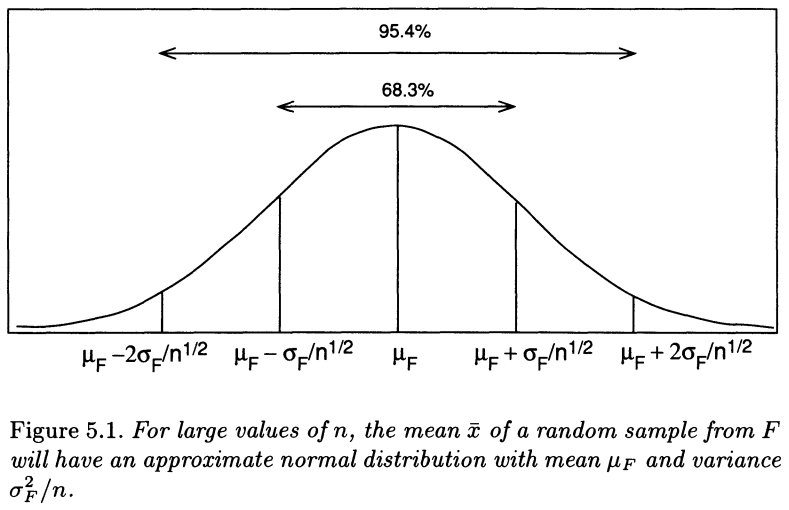
\includegraphics[width=\linewidth]{4/f51.png}
\newline
Простой пример показывает ограничения аппроксимации центральной предельной теоремы. Предположим, что $F$ -- это распределение, которое ставит вероятность только для двух исходов, 0 или 1, скажем 
\begin{equation}
    Prob\{x=1\}=p\qquad Prob\{x=0\}=1-p.
\end{equation}
Здесь $p$ -- параметр $F$, часто называемый вероятностью успеха, имеющий значение от 0 до 1. Случайная выборка $F \rightarrow (x_1, x_2,\cdots, x_n)$ может рассматриваться как $n$ независимых подбрасываний монеты с вероятностью успеха (или «орла», или $x = 1$) равной $p$. Тогда сумма $s = \sum_{i=1}^nx_i$ -- количество успехов в $n$ независимых бросках монеты; $s$ имеет биномиальное распределение (3.3), 
\begin{equation}
    s\sim Bi(n,p).
\end{equation}
Среднее значение $\bar x = s / n$ равно $\hat p$ в плагин оценке $p$ Распределение (5.7) имеет $\mu_F=p$, $\sigma^2_F = p (1- p)$, поэтому (5.3) дает 
\begin{equation}
    \hat p\sim (p,p(1-p)/n)
\end{equation}

для среднего и дисперсии $\hat p$ Другими словами, $\hat p$ -- это несмещенная оценка $p$, $E (\hat p) = p$, со стандартной ошибкой 
\begin{equation}
    se(\hat p)=\left[\frac{p(1-p)}{n}\right]^{1/2}.
\end{equation}
\newline

\noindent
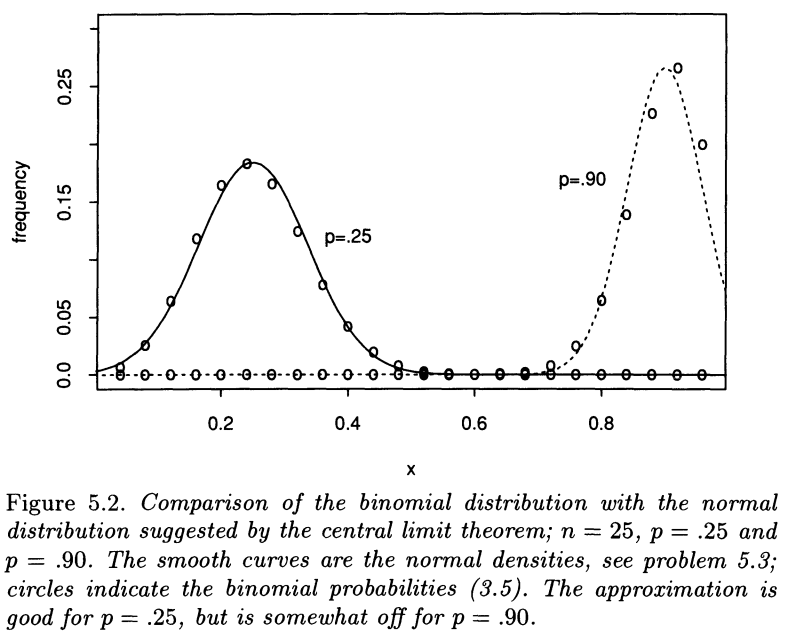
\includegraphics[width=\linewidth]{4/f52.png}
\newline
На рис. 5.2 показана центральная предельная теорема, работающая для биномиального распределения при $n = 25$, $p = 0.25$ и $p = 0.90$. Центральная предельная теорема дает хорошее приближение к биномиальному распределению для $n = 25$, $p = 0.25$, но несколько хуже для $n = 25$, $p = 0.9$. 
\section{Оценка стандартной ошибки среднего}

Предположим, что у нас есть случайная выборка чисел $F \rightarrow x_1, x_2, \cdots, x_n$, например контрольные измерения $n = 9$ для данных о мышах из таблицы 2.1. Мы вычисляем оценку $\bar x$ для математического ожидания $\mu_F$, равного 56.22 для данных о мышах, и хотим знать стандартную ошибку $\bar x$. Формула (5.4) $se_F (\bar x) = \sigma_F/\sqrt{n}$ включает неизвестное распределение $F$ и поэтому не может использоваться напрямую. 

На этом этапе мы можем использовать принцип плагина: мы подставляем $\hat F$ вместо $F$ в формуле $se_F (\bar x) = \sigma_F/\sqrt{n}$. Плагин оценка $\sigma_F = [E_F (x- \mu_F)^2]^{1/2}$ равна
\begin{equation}
    \hat\sigma=\sigma_{\hat F}=\{\frac{1}{n}\sum_{i=1}^n(x_i-\bar x)^2\}^{1/2},
\end{equation}
поскольку $\mu_{\hat F}= \bar x$ и $E_{\hat F}g (x) = \frac{1}{n}\sum_{i=1}^n g (x_i)$ для любой функции $g$. Это дает оценку стандартной ошибки $\widehat{se} (\bar x) = se_{\hat F} (\bar x)$, 
\begin{equation}
    \widehat{se} (\bar x) = \sigma_{\hat F}/\sqrt{n}=\{\sum_{i=1}^n(x_i-\bar x)^2/n^2\}^{1/2}.
\end{equation}
Для контрольной группы данных о мышах $\widehat{se} (\bar x) = 13.33$.

Формула (5.12) немного отличается от обычной оценки стандартной ошибки (2.2). Это потому, что $\sigma_F$ обычно оценивается как $\bar\sigma=\{\sum(x_i-\bar x)^2/(n-1)\}^{1/2}$, а не как $\hat\sigma$, (5.11). Деление на $n - 1$ вместо $n$ делает $\bar\sigma^2$ несмещенной для $\sigma_F^2$. Для большинства целей $\hat\sigma$ так же хороша, как $\bar\sigma$ для оценки $\sigma_F$. 

Обратите внимание, что мы использовали принцип плагина дважды: сначала для оценки математического ожидания $\mu_F$ с помощью $\mu_{\hat F} = \bar x$, а затем для оценки стандартной ошибки $se_F (\bar x)$ с помощью $se_{\hat F} (\bar x)$. Бутстреп оценка стандартной ошибки, о которой идет речь в главе 6, сводится к использованию принципа плагина для оценки стандартной ошибки произвольной статистики $\hat\theta$. Здесь мы видели, что если $\hat\theta = \bar x$, то этот подход приводит к (почти) обычной оценке стандартной ошибки. Как мы увидим, преимущество бутстрепа в том, что его можно применить практически к любой статистике $\hat\theta$, а не только к среднему значению $\bar x$. 

\chapter{Бутстреп оценка стандартной ошибки}
\section{Введение}

Предположим, мы находимся в следующей общей ситуации анализа данных: была обнаружена случайная выборка $\mathbf{x} = (x_1, x_2, \cdots, x_n)$ из неизвестного распределения вероятностей $F$, и мы хотим оценить интересующий параметр $\theta = t (F)$ на основе $\mathbf{x}$. Для этого мы вычисляем оценку $\hat\theta = s (\mathbf{x})$ из $\mathbf{x}$. [Обратите внимание, что $s (\mathbf{x})$ может быть плагин оценкой $t (\hat F)$, но это не обязательно.] Насколько точна $\hat\theta$? Бутстреп был представлен в 1979 году как компьютерный метод оценки стандартной ошибки $\hat\theta$. Он имеет то преимущество, что он полностью автоматический. Самостоятельная оценка стандартной ошибки не требует теоретических вычислений и доступна независимо от того, насколько математически сложной может быть оценка $\hat\theta = s (\mathbf{x})$. Это описано и проиллюстрировано в этой главе. 
\section{Бутстреп оценка стандартной ошибки}

Бутстреп методы зависят от понятия бутстреп выборки. Пусть $\hat F$ -- эмпирическое распределение, присваивающее вероятность $1 / n$ на каждое из наблюдаемых значений $x_i$, $i = 1, 2,\cdots, n$, как описано в главе 4. Бутстреп выборка является случайной выборкой размера $n$, набранной из $\hat F$, скажем, $\mathbf{x}^* = (x_1^*, x_2^*, \cdots, x_n^*)$,
\begin{equation}
    \hat F\rightarrow (x_1^*, x_2^*, \cdots, x_n^*).
\end{equation}
<<*>> указывает, что $\mathbf{x}^*$ не является фактическим набором данных $\mathbf{x}$, а скорее рандомизированной или перезапущенной версией $\mathbf{x}$.

Есть еще один способ сказать (6.1): точки бутстреп данных $x_1^*, x_2^*, \cdots, x_n^*$ являются случайной выборкой размера $n$, выбранной с заменой из совокупности $n$ объектов $(x_1, x_2, \cdots, x_n )$. Таким образом, мы могли бы иметь $x_1^* = x_7, x_2^* = x_3, x_4^* = x_3, x_4^* = x_{22},\cdots, x_n^* = x_7$. Набор бутстреп данных $(x_1^*, x_2^*, \cdots, x_n^*)$ состоит из элементов исходного набора данных $(x_1, x_2,\cdots, x_n)$, некоторые из которых появляются ноль раз, некоторые появляются один раз, некоторые появляются дважды, и так далее.

В соответствии с набором бутстреп данных $\mathbf{x}^*$, бутстреп репликация $\hat\theta$ -- это
\begin{equation}
    \hat\theta^*=s(\mathbf{x}^*).
\end{equation}
Величина $s(\mathbf{x}^*)$ является результатом применения той же функции $s (\cdot)$ к $\mathbf{x}^*$, которая была применена к $\mathbf{x}$. Например, если $s(\mathbf{x})$ является выборочным средним значением $\bar x$, то $s(\mathbf{x}^*)$ -- это среднее значение набора бутстреп данных, $\bar x^*=\sum_{i=1}^nx_i^*/n$. 

Бутстреп оценка $se_F (\hat\theta)$ стандартной ошибки статистики $\hat\theta$ представляет собой плагин оценку, которая использует эмпирическую функцию распространения $\hat F$ вместо неизвестного распределения $F$. В частности, бутстреп оценка  $se_F (\hat\theta)$ определяется, как 
\begin{equation}
    se_{\hat F} (\hat\theta^*).
\end{equation}
Другими словами, бутстреп оценка $se_F (\hat\theta)$ является стандартной ошибкой $\hat\theta$ для наборов данных размером $n$, случайным образом выбранных из $\hat F$. 

Формула (6.3) называется идеальной бутстреп оценкой ошибки $\hat\theta$. К сожалению, для практически любой оценки $\hat\theta$, кроме среднего, нет точной формулы (5.4), которая позволяет вычислить числовое значение идеальной оценки точно. Бутстреп алгоритм, описанный ниже, является вычислительным способом получения хорошего приближения к численному значению $se_{\hat F} (\hat\theta^*)$. 

Легко реализовать бутстреп выборку на компьютере. Устройство выбирает случайные целые числа $i_1, i_2, \cdots, i_n$, каждое из которых равняется любому значению между 1 и $n$ с вероятностью $1 / n$. Бутстреп выборка состоит из соответствующих членов $\mathbf{x}$,
\begin{equation}
    x_1^*=x_{i_1},x_2^*=x_{i_2},\cdots,x_n^*=x_{i_n}.
\end{equation}

Бутстреп алгоритм работает путем выбора множества независимых бутстреп выборок, оценки соответствующих бутстреп репликаций и оценки стандартной ошибки $\hat\theta$ через эмпирическое стандартное отклонения репликаций. Результат называется бутстреп оценкой стандартной ошибки, обозначенной $\widehat{se}_B$, где $B$ -- количество используемых бутстреп выборок.

Алгоритм 6.1 -- это более явное описание бустреп процедуры для оценки стандартной ошибки $\hat\theta=s(\mathbf{x})$ из наблюдаемых данных $\mathbf{x}$. 

\newpage
\begin{center}
    \textit{Алгоритм 6.1}
    
    \underline{Бутстреп алгоритм для оценки стандартных ошибок}
    
    \begin{enumerate}
        \item Выберите $B$ независимых бутстреп выборок $x^{*1}, x^{*2},\cdots, x^{*B}$, каждый из которых состоит из $n$ точек данных, выбранных с заменой их $\mathbf{x}$, как в (6.1) или (6.4). [Для оценки стандартной ошибки B обычно будет в диапазоне 25-200, см. Таблицу 6.1.] 
        
        \item Оцените бутстреп репликацию, соответствующую каждой бутстреп выборке,
        \begin{equation}
            \hat\theta^*(b)=s(\mathbf{x}^{*b})\qquad b=1,2,\cdots,B.
        \end{equation}
        
        \item Оцените стандартную ошибку $se_F (\hat\theta)$ через выборочное стандартное отклонение $B$ репликаций 
        \begin{equation}
            \widehat{se}_B=\left\{\sum_{b=1}^B[\hat\theta^*(b)-\hat\theta^*(\cdot)]^2/(B-1)\right\}^{1/2},
        \end{equation}
        где $\hat\theta^*(\cdot)=\sum_{b=1}^B\hat\theta^*(b)/B$.
    \end{enumerate}
\end{center}

На рисунке 6.1 изображена схематическая диаграмма бутстреп алгоритма стандартных ошибок. 

Предел $\widehat{se}_B$ по $B$ стремится к бесконечности -- это идеальная бутстреп оценка $se_F(\hat\theta)$,
\begin{equation}
    \lim_{B\rightarrow\infty}\widehat{se}_B=se_{\hat F}=se_{\hat F}(\hat\theta^*).
\end{equation}
Тот факт, что $\widehat{se}_B$ стремится к $se_{\hat F}$ при $B$, стремящимся к бесконечности, позволяет сказать, что эмпирическое стандартное отклонение приближается к стандартному отклонению совокупности с увеличением количества репликаций. «Совокупность» в этом случае является совокупностью значений $\hat\theta^*=s(\mathbf{x}^*)$, где $\hat F \rightarrow (x_1^*, x_2^*, \cdots, x_n^*) = \mathbf{x}^*$. 

Идеальная бутстреп оценка $se_{\hat F}\hat\theta^*$ и его приближение $\widehat{se}_B$ иногда называют непараметрическими бутстреп оценками, потому что они основаны на $\hat F$, непараметрической оценке $F$. В разделе 6.5 мы обсуждим параметрический бутстреп, который использует другую оценку F. 

Немного об обозначениях: в (6.7) мы пишем $se_{\hat F}(\hat\theta^*)$, а не $se_{\hat F}(\hat\theta)$, чтобы избежать путаницы между $\hat\theta$, значением $s (\mathbf{x})$ на основе наблюдаемых данных, и $\hat\theta^* = s (\mathbf{x}^*)$, случайной величиной на основе бутстреп выборки. Более подробное обозначение $se_{\hat F} (\hat\theta (\mathbf{x}^*))$ подчеркивает, что $se_{\hat F}$ является бутстрепированной стандартной ошибкой: фактические данные $\mathbf{x}$ остаются фиксированным в (6.7); Случайность в расчете исходит из изменчивости бутстреп выборок $\mathbf{x}^*$ для данного x. Точно так же мы будем писать $E_{\hat F}g(\mathbf{x^*})$, чтобы указать бутстрепированное математическое ожидание функции $g (\mathbf{x}^*)$: математическое ожидание с фиксированным $\mathbf{x}$ (и $\hat F$) и случайным $\mathbf{x}^*$ в соответствии с (6.1). 
\newline

\noindent
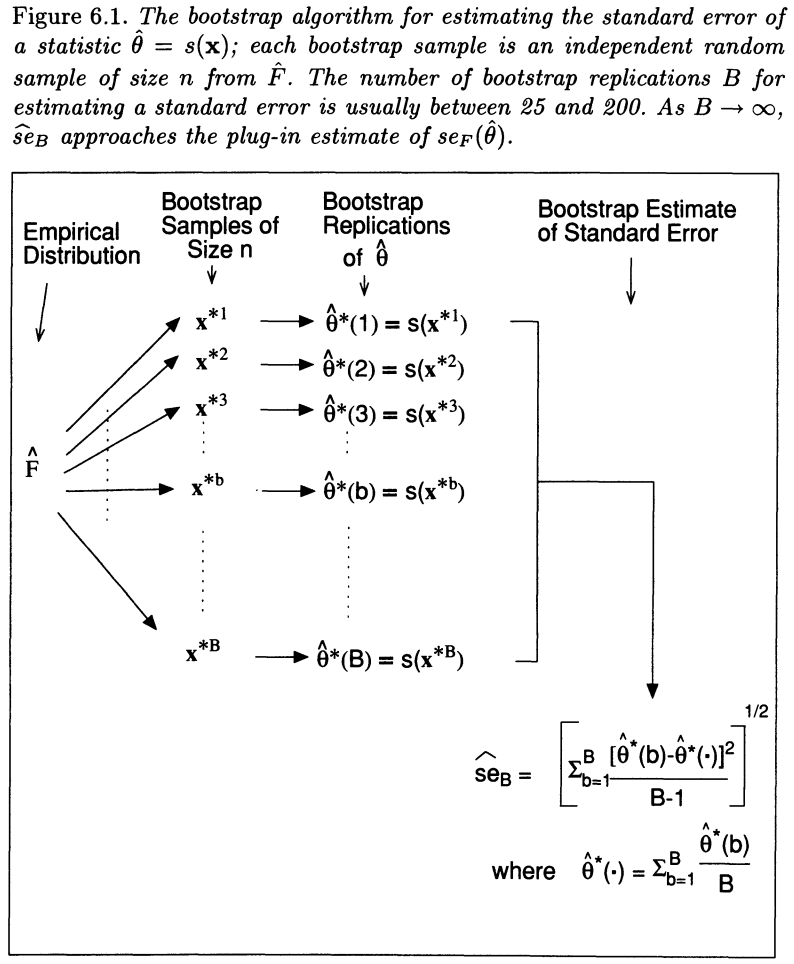
\includegraphics[width=\linewidth]{5/f61.png}
\newline

Всего существует $C_n^{2n-1}$ различных бутстреп выборок. Обозначим их через $z^1, z^2, \ldots z^m$, где $m = C_n^{2n-1}$. Например, если $n = 2$, отдельными выборками являются $(x_1, x_1)$, $(x_2, x_2)$ и $(x_1, x_2)$; поскольку порядок не имеет значения, $(x_2, x_1)$ совпадает с $(x_1, x_2)$. Вероятность получения одной из этих выборок при выборе с заменой может быть получена из полиномиального распределения. Обозначим вероятность $j$-й выборки через $\omega_j, j = 1, 2, \ldots C_n^{2n-1}$. Тогда прямым способом вычисления идеальной бутстреп оценки стандартной ошибки будет использование стандартного отклонения совокупности m бутстреп значений $s (z^j)$:
\begin{equation}
    se_{\hat F}(\hat\theta^*)=[\sum_{j=1}^m\omega_j\{s(z^j)-s(\cdot)\}^2]^{1/2}
\end{equation}
где $s (\cdot) = \sum_{j=1}^m\omega_js(z^j)$. Сложность этого подхода заключается в том, что, если $n$ не достаточно мало $(\le 5)$, число $C_n^{2n-1}$ очень велико, что делает вычисление (6.8) непрактичным. Отсюда необходимость в бутстрап выборкaх, описаных выше. 
\section{Пример: коэффициент корреляции}

Мы уже видели два примера бутстреп оценок стандартной ошибки для среднего и медианного значения для экспериментальной группы данных о мышах, таблица 2.1. В качестве второго примера рассмотрим выборочный коэффициент корреляции между $y = LSAT$ и $z = GPA$ для $n = 15$ точек данных о юридических школах, таблица 3.1, $\widehat{corr}(y, z) =0.776$. Насколько точна оценка $0.776$? В таблице 6.1 показана бутстреп оценка стандартной ошибки $\widehat{se}_B$ для $B$ в диапазоне от $25$ до $3200$. Последнее значение, $\widehat{se}_{3200} = 0.132$, является нашей оценкой $se_F (\widehat{corr})$. Позже мы увидим, что $\widehat{se}_{200}$ почти так же хороша для оценки $se_F$, как $\widehat{se}_{3200}$· 

Глядя на правую часть рисунка 3.1, читатель может представить себе, как работает генерация бутстреп выборок. Выборочная корреляция по $n = 15$ исходным точкам данных составляет $\widehat{corr} = 0.776$. Бутстреп выборка состоит из $15$ точек, выбранных случайным образом и заменяющих исходные $15$. Корреляция бутстреп выборки представляет собой бутстреп репликацию $\widehat{corr}^*$, которая может быть больше или меньше, чем $\widehat{corr}$. Независимые повторения генерации бутстреп выборок дают бутстреп репликации $\widehat{corr}^*(1),\widehat{corr}^*(2),\cdots,\widehat{corr}^*(B)$. Наконец, $\widehat{se}_B$ -- выборочное стандартное отклонение значений $\widehat{corr}^*(b)$. 
\newline

\noindent
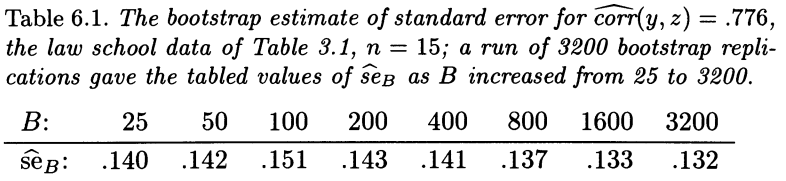
\includegraphics[width=\linewidth]{5/t61.png}
\newline

Левая панель рисунка 6.2 представляет собой гистограмму $3200$ бутстреп репликаций $\widehat{corr}^*(b)$. Всегда рекомендуется просматривать бутстреп данные графически, а не полагаться полностью на одну сводную статистику, такую как $\widehat{se}_B$. В примере корреляции может оказаться, что несколько выпадающих значений $\widehat{corr}^*(b)$ сильно раздувают $\widehat{se}_B$, и в этом случае стоит использовать более надежную меру стандартного отклонения; Выводы, основанные на нормальной кривой, как в (5.6) и на рисунке 5.1, сомнительны, когда бутстреп гистограмма явно ненормальна.

В примере с юридическими школами у нас есть полная совокупность $\mathbf{X}$ из $N = 82$ школ, Таблица 3.2. В правой части рисунка 6.2 показана гистограмма $\widehat{corr} (y, z)$ для $3200$ выборок размера $n = 15$, взятых из $\mathbf{X}$. Другими словами, $3200$ случайных выборок $\mathbf{x} = (x_1, x_2, \cdots, x_{15})$ были составлены с заменой из $82$ точек в $\mathbf{X}$, и $\widehat{corr}(\mathbf{x})$ оценивался для каждого из них. Стандартное отклонение $3200$ значений $\widehat{corr}(\mathbf{x})$ составило $0.131$, таким образом $\widehat{se}_B$ является хорошей оценкой стандартной ошибки генеральной совокупности. Что еще более впечатляюще, бутстреп гистограмма слева сильно напоминает гистограмму справа. Помните, что в реальной проблеме у нас была бы только информация слева, из которой мы пытались бы вывести ситуацию справа. 
\newline

\noindent
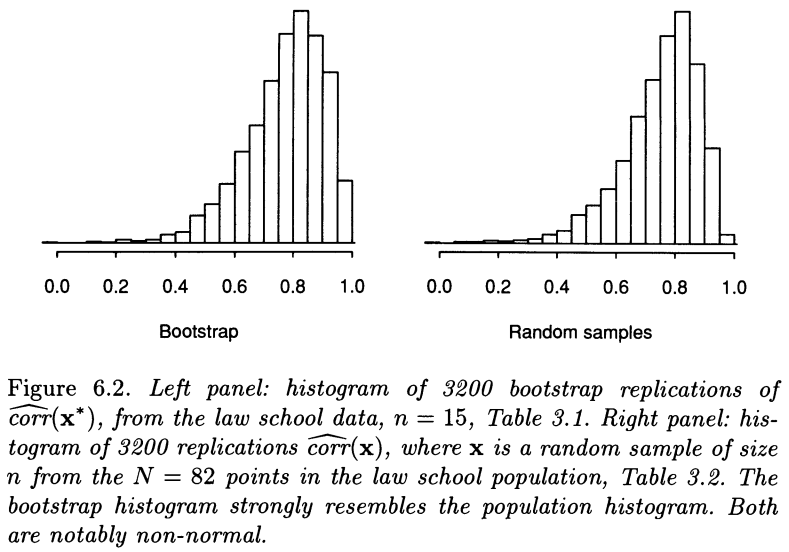
\includegraphics[width=\linewidth]{5/f62.png}
\newline
\section{Количество бутстреп репликаций $B$}

Насколько большим мы должны взять $B$, количество бутстреп репликаций, используемых для оценки $\widehat{se}_B$? Идеальная бутстреп оценка $\widehat{se}_\infty$ использует $B=\infty$, и в этом случае $\widehat{se}_\infty$ равно плагин оценке $se_{\hat F}(\hat\theta^*)$. Формула (5.12) дает $\widehat{se}_\infty$ для $\hat\theta=\bar x$, но для большинства других статистических данных мы должны фактически выполнить генерацию бутстреп выборок. Время, затрачиваемое компьютером, которое в основном зависит от того, сколько времени требуется для оценки бутстреп репликаций (6.5), линейно увеличивается с $B$. Временные ограничения могут диктовать небольшое значение $B$, если $\hat\theta = s (\mathbf{x})$ -- очень сложная функция.

Нам нужно такое же хорошее поведение от оценки стандартной ошибки, что и от оценки любой другой интересующей величины: небольшая систематическая ошибка и небольшое стандартное отклонение. Бутстреп оценка стандартной ошибки обычно имеет относительно небольшое смещение. Идеальная начальная оценка $\widehat{se}_\infty$ имеет наименьшее возможное стандартное отклонение среди почти несмещенных оценок $se_F(\hat\theta)$, по крайней мере, в асимптотическом $(n \rightarrow\infty)$ смысле. Эти хорошие свойства вытекают из того факта, что $\widehat{se}_\infty$ -- это плагин оценка $se_{\hat F}(\hat\theta)^*$. Нетрудно показать, что $\widehat{se}_B$ всегда имеет большее стандартное отклонение, чем $\widehat{se}_\infty$. Практический вопрос: насколько большее?

Приблизительный, но вполне удовлетворительный ответ можно сформулировать в терминах коэффициента вариации $\widehat{se}_B$, отношения стандартного отклонения $\widehat{se}_B$ к его математическому ожиданию. Повышенная изменчивость из-за остановки после $B$ бутстреп репликаций, а не бесконечности, отражается в увеличенном коэффициенте вариации,
\begin{equation}
    cv(\widehat{se}_B)=\left\{cv(\widehat{se}_\infty)^2+\frac{E(\Delta)+2}{4B}\right\}^{1/2}.
\end{equation}
Здесь $\Delta$ -- параметр, который измеряет, насколько длиннохвостым является распределение $\hat\theta^*$: если $\Delta$ равно нулю для нормального распределения, оно колеблется от $-2$ для короткохвостых распределений до произвольно больших значений, когда F длиннохвостное. На практике $\delta$ обычно не превышает $10$. Коэффициент вариации в уравнении (6.9) относится к вариации как на уровне повторных выборок (бутстреп), так и на уровне исходной выборки. Идеальная оценка $\widehat{se}_\infty = se_{\hat F}(\hat\theta^*)$ не идеальна. Она все еще может иметь значительную изменчивость в качестве оценки $se_F(\hat\theta)$ из-за изменчивости $\hat F$ как оценки $F$. Например, если $x_1, x_2, \cdots, x_n$ является случайной выборкой из нормального распределения и $\hat\theta=\bar x$, тогда $cv(\widehat{se}_\infty)=1/\sqrt{2n}$, равное $0.22$ для n = 10. Формула (6.9) имеет важное практическое следствие: для значений $cv(\widehat{se}_\infty)$ и $\Delta$, которые могут возникнуть на практике, $cv(\widehat{se}_B)$ не намного больше, чем $cv(\widehat{se}_\infty)$ для $B\ge 200$. 

Таблица 6.2 сравнивает $cv(\widehat{se}_B)$ с $cv(\widehat{se}_\infty)$ для различных вариантов $B$, предполагая $\Delta = 0$. Очень часто можно ожидать, что $cv(\widehat{se}_\infty)$ будет не меньше, чем $0.10$, и в этом случае $B = 100$ дает вполне удовлетворительные результаты.
\newline

\noindent
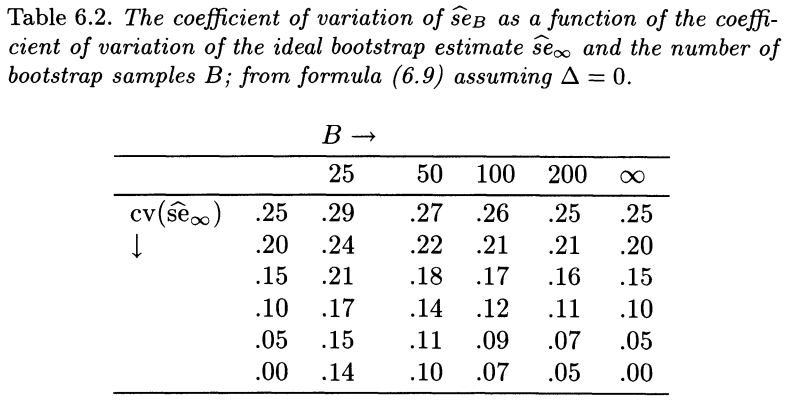
\includegraphics[width=\linewidth]{5/t62.png}
\newline
Вот два практических правила, взятых из опыта:
\begin{enumerate}
    \item Даже небольшое количество бутстреп репликаций, скажем, $B = 25$, обычно является информативным. $B = 50$ часто бывает достаточно, чтобы дать хорошую оценку $se_F (\hat\theta)$.
    \item Очень редко для оценки стандартной ошибки требуется более $B = 200$ репликаций. (Для доверительных бутстреп интервалов требуются гораздо большие значения $B$.) 
\end{enumerate}

Аппроксимации, полученные путем случайной выборки или моделирования, называются оценками Монте-Карло. Вычислительные методы, отличные от прямого моделирования Монте-Карло, иногда могут во много раз сократить количество повторений $B$, необходимых для достижения заданной точности. Между тем стоит помнить, что бутстреп данные, как и реальные данные, заслуживают внимательного изучения. В частности, отображение гистограммы бутстреп репликаций почти никогда не бывает пустой тратой времени. 
\section{Параметрический бутстреп}

Может показаться странным использование бутстреп алгоритма для оценки стандартных ошибок, когда можно использовать формулу из учебника. Фактически, бутстреп выборки могут генерироваться параметрически, в этом случае результаты тесно связаны с формулами стандартных ошибок из учебников. 

Параметрическая бутстреп оценка стандартной ошибки определяется как 
\begin{equation}
    se_{\hat F_{par}}(\hat\theta^*),
\end{equation}
где $\hat F_{par}$ -- оценка $F$, полученная из параметрической модели данных. Здесь мы приведем простой пример, чтобы проиллюстрировать идею. Для данных о юридических школах, вместо оценки $F$ эмпирическим распределением $\hat F$, мы могли бы предположить, что популяция имеет двумерное нормальное распределение. Разумные оценки среднего значения и ковариации этой совокупности даны как $(\bar y, \bar z)$ и
\begin{equation}
    \frac{1}{14}\left(
    \begin{array}{cc}
        \sum(y_i-\bar y)^2 & \sum(y_i-\bar y)(z_i-\bar z) \\
        \sum(y_i-\bar y)(z_i-\bar z) & \sum(z_i-\bar z)^2
    \end{array}
    \right).
\end{equation}
Обозначим двумерную нормальную популяцию с этим средним значением и ковариацией как $\hat F_{norm}$; это пример параметрической оценки совокупности $F$. Используя это, параметрическая бутстреп оценка стандартной ошибки корреляции $\hat\theta$ является $se_{\hat F_{norm}} (\hat\theta^*)$. Как и в непараметрическом случае, идеальная параметрическая бутстреп оценка не может быть легко вычислена, за исключением тех случаев, когда $\hat\theta$ является средним. Поэтому мы аппроксимируем идеальную бутстреп оценку с помощью бутстреп выборок, но другим способом, чем раньше. Вместо выборок с заменой из исходных данных мы берем $B$ выборок размера $n$ из параметрической оценки генеральной совокупности $\hat F_{par}$:
\begin{equation}
    \hat F_{par}\rightarrow(x_1^*,x_2^*,\ldots,x_n^*).
\end{equation}
После генерации бутстреп выборок мы действуем точно так же, как в шагах 2 и 3 бутстреп алгоритма из раздела 6.2: мы оцениваем нашу статистику для каждой бутстреп выборки, а затем вычисляем стандартное отклонение $B$ бутстреп репликаций.

В примере с коэффициентом корреляции, предполагая двумерную нормальную совокупность, мы берем $B$ выборок размером $15$ из $\hat F_{norm}$ и вычисляем коэффициент корреляции для каждой бутстреп выборки. На левой панели рисунка 6.3 показана гистограмма для $B = 3200$ бутстреп репликаций, полученных таким образом. Это очень похоже на гистограммы на рисунке 6.2. Параметрическая бутстреп оценка стандартной ошибки для этих повторений была $0.124$, что близко к значению $0.131$, полученному на непараметрических бутстреп выборках.

Учебная формула для стандартной ошибки коэффициента корреляции составляет $(1-\hat\theta^2) / \sqrt{n- 3}$. Подставляя $\hat\theta = 0.776$, она дает значение $0.15$ для данных о юридических школах.
\newline

\noindent
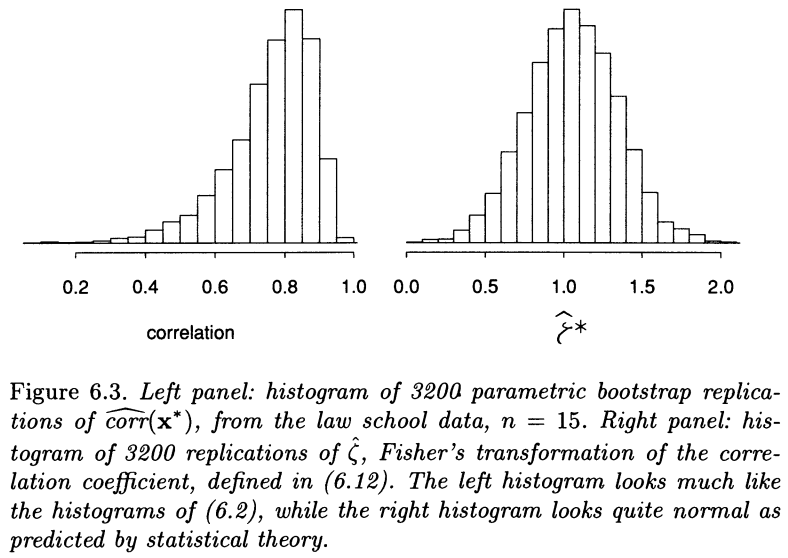
\includegraphics[width=\linewidth]{5/f63.png}
\newline
Мы можем провести дальнейшее сравнение с нашим параметрическим бутстреп результатом. Учебные материалы также утверждают, что преобразование Фишера, примененное к $\hat\theta$
\begin{equation}
    \hat\zeta=0.5\log\left(\frac{1+\hat\theta}{1-\hat\theta}\right)
\end{equation}
приблизительно нормально распределено со средним $\zeta= 0.5  \log\left(\frac{1+\theta}{1-\theta}\right)$ и стандартным отклонением $1 / \sqrt{n-3}$, где $\theta$ является коэффициентом корреляции совокупности. Исходя из этого, обычно выполняется вывод для $\zeta$ и затем преобразуется обратно, чтобы сделать вывод о коэффициенте корреляции. Чтобы сравнить это с нашим параметрическим бутстреп анализом, мы вычислили $\hat\zeta$ вместо $\hat\theta$ для каждой из наших $3200$ бутстреп выборок. Гистограмма значений $\hat\zeta^*$ показана на правой панели рисунка 6.3 и выглядит вполне нормально. Кроме того, стандартное отклонение $3200$ значений $\hat\zeta^*$ было $0.290$, что очень близко к значению $1 / \sqrt{15-3} = 0.289$. 

Это соглашение выполняется в целом. Большинство формул для стандартных ошибок в учебниках являются приближениями, основанными на нормальной теории, и обычно дают ответы, близкие к параметрическому бутстрепу, который отбирает выборки из нормального распределения. Взаимосвязь между бутстрепом и традиционной статистической теорией -- более сложная математическая тема.

У бутстрепа есть два несколько отличных друг от друга преимущества по сравнению с традиционными методами из учебников: 1) при использовании в непараметрическом режиме он избавляет аналитика от необходимости делать параметрические предположения о форме базовой совокупности, и 2) при использовании в параметрическом режиме он обеспечивает болле точные ответы, чем формулы из учебника, и могут дать ответы на задачи, для которых не существует формул из учебника. 

Большая часть этого пособия сосредоточена на непараметрическом применении бутстрепа. Параметрический бутстреп полезен в задачах, где доступны некоторые знания о форме генеральной совокупности, а также для сравнение с непараметрическим анализом. Однако основная причина использования параметрических допущений в традиционном статистическом анализе состоит в том, чтобы облегчить вывод формул для стандартных ошибок из учебников. Поскольку нам не нужны формулы в бутстреп подходе, мы можем избежать ограничительных параметрических предположений. 


\chapter{Бутстреп и стандартные ошибки: некоторые примеры}
\section{Введение}

До внедрения компьютеров вычисляли стандартные ошибки используя методы математического анализа и предположения о распределении, что часто предполагало много работы на механических калькуляторах. Один такой классический результат был дан в разделе 6.5: он относится к выборочному коэффициенту корреляции $\widehat{\text{corr}}(y,z)$ (4.6). Если сделать предположение о том, что $n$ элементов выборки $(y_i,z_i)$ взяты из двумерного нормального распределения с функцией распределения $F$, тогда разумной оценкой стандартной ошибки $\widehat{\text{corr}}$ будет
\begin{equation}
	\widehat{\text{se}}_\text{normal} = (1 - \widehat{\text{corr}}^2)/\sqrt{n-3}
\end{equation}

Ясно, что может последовать возражение относительно использования двумерного нормального распределения: на каком основании делается предположение о том, что $F$ подчиняется нормальному закону? Для намётанного глаза точки на правом графике рисунка 3.1 не выглядят взятыми из нормального распределения --- точка с координатами $(576, 3.39)$ кажется слишком далёкой от остальных 14 точек. На самом деле, главная причина выбора двумерного нормального распределения --- простота оценивания. Другое предположение не привело бы к такой простой оценкe для $\text{se}(\widehat{\text{corr}})$.

Есть ещё одно серьёзное возражение против 
$
\widehat{\text{se}}_\text{normal}:
$
требуется приложить серьёзные усилия для того, чтобы вывести формулу наподобие (7.1). Если выбрать чуть более сложную статистику, чем $\widehat{\text{corr}},$ или же менее стандартное распределение, то никакие математические трюки не приведут к простой формуле. Ввиду таких ограничений, до-компьютерная статистика в качестве объектов интереса рассматривала  в основном небольшие классы распределений и ограниченный набор статистик. Компьютерные методы, такие как бутстреп, освобождают статистика от таких ограничений. Стандартные ошибки, равно как и другие статистические меры точности, получаются в результате процедуры автоматически, безотносительно к математической сложности.\footnote{В таком подходе есть не только плюсы. Теоретические формулы наподобие (7.1) могут помочь нам понимать ситуацию немного иначе, чем при получении численных результатов применения bootstrap. Хорошо иметь в виду, что такие методы, как bootstrap, освобождают статистика от необходимости смотреть на данные \textit{более} глубоко, без страха усложнений в математике, но не \textit{менее}.}

Бутстреп методы оказываются очень полезными в сложных проблемах оценивания. В этой главе обсуждаются стандартные ошибки для двух таких задач: первая касается собственных значений и собственных векторов матрицы ковариаций, вторая --- алгоритма \textit{loess} приближения функций. Разъяснение данных задач требует знакомства с матричной терминологией, однако здесь это будет опущено; в любом случае эта теория не является необходимой для того, чтобы понять главную идею: что простой алгоритм бутстрепа позволяет находить стандартные ошибки для очень трудных случаев.
 
\section{Пример 1: результаты тестов}
В таблице 7.1 показаны данные результатов тестов из Mardia, Kent and Bibby (1979); $n = 88$ студентов сдавали пять тестов: по механике, векторному исчислению, алгебре, математическому анализу, и статистике.

На первых двух тестах не разрешалось использовать учебник, на остальных учебник был разрешён. Удобно представлять эти данные как матрица  данных $\mathbf X$ размерности $88 \times 5$, где $i$-ая строка есть
\begin{equation}
	\mathbf x_i = (x_{i1}, x_{i2}, x_{i3}, x_{i4}, x_{i5})
\end{equation}
--- пять результатов $i$-го студента, $i = 1,2,\ldots,88.$

Вектор средних $\bar{\mathbf{x}} = \sum_{i = 1}^{88} \mathbf{x}_i/88$ есть вектор средних по столбцам:
\begin{equation}
	\bar{\mathbf x} = (38.95, 50.59, 50.60, 46.68, 42.31).
\end{equation}
 Эмпирическая ковариационная матрица $\mathbf G$ --- это матрица $5 \times 5$, где $(j, k)$-й элемент равен
 
\begin{equation}
G_{jk} = \frac{1}{88}\sum_{i = 1}^{88} (x_{ij} - \bar x_j) (x_{ik} - \bar x_k) \qquad j,k = 1,2,3,4,5.
\end{equation}

Заметим, что диагональные элементы $G_{jk}$ это оценки дисперсии результатов теста $j$ методом подстановки. Получим матрицу
\newline
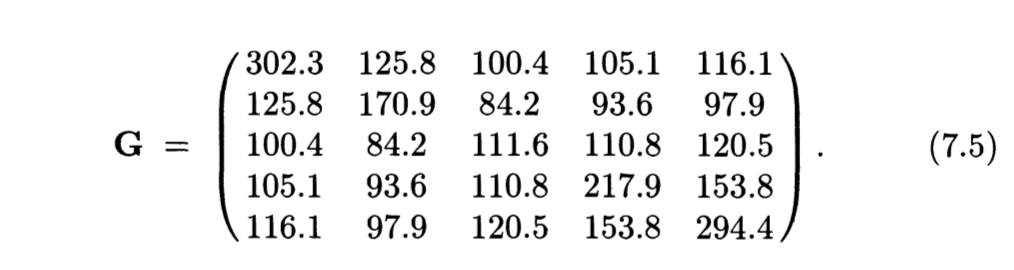
\includegraphics[width=0.85\linewidth]{6/e75.png}
\newline

\setcounter{equation}{5}
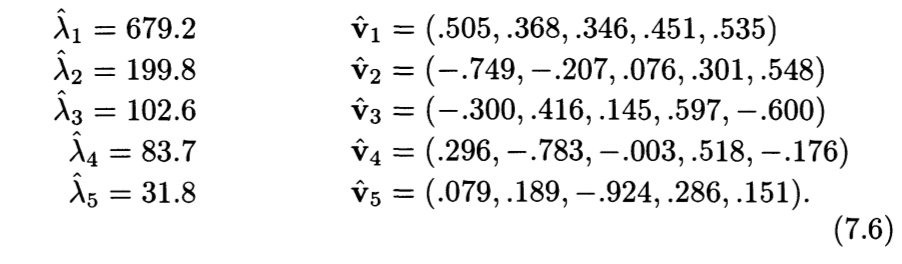
\includegraphics[width=0.85\linewidth]{6/e76.png}
\newline

\setcounter{equation}{6}
Какой интерес представляют собственные значения и векторы ковариационной матрицы? Они помогают описать структуру высокоразмерных данных (как в случае с таблицей (7.1)) в которых описано большое число независимых величин ($n = 88$ студентов), но при этом имеются коррелированные измерения для каждого студента. Заметьте, что пять тестовых оценок высоко коррелированы. Студент, который хорошо сдал тест по механике, вероятно также хорошо сдал тест и по векторам и т.д. Очень простая модель для коррелированных оценок имеет вид
\begin{equation}
	\mathbf x_i = Q_i \mathbf v, \qquad i = 1,2,\ldots,88.
\end{equation}

\noindent
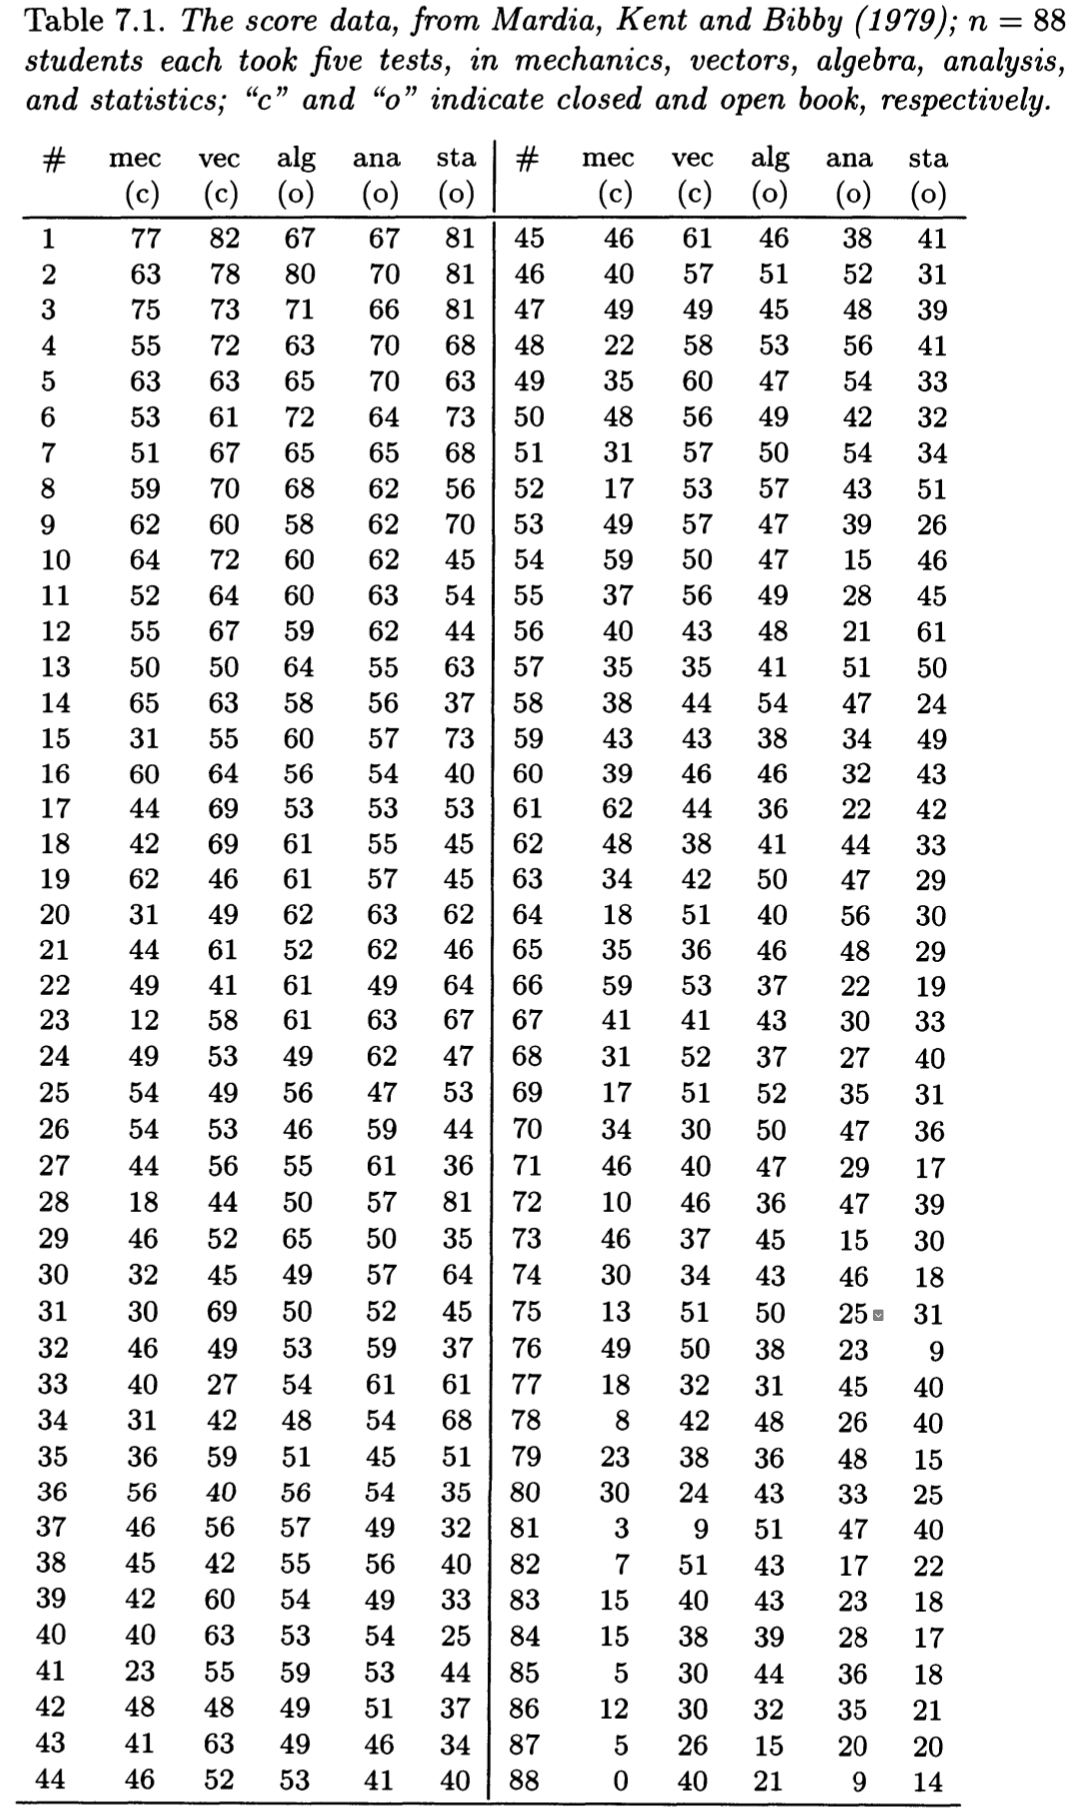
\includegraphics[width=0.9\linewidth]{6/t71.png}
\newline
\setcounter{table}{1}

$Q_i$ является числом, представляющим способности $i$-го студента, в то время как $\mathbf v = (v_1,v_2,v_3,v_4,v_5)$ есть фиксированный вектор из 5 чисел, определённый для всех студентов. $Q_i$ можно рассматривать как общую оценку интеллектуальных способностей студента $i$ (IQ). Изначально IQ были мотивированы именно моделями чуть сложнее, чем (7.7).

Если бы модель (7.7) была верна, мы бы смогли это определить из собственных значений: только $\hat \lambda_1$ было бы положительным, остальные --- $\hat \lambda_2, \hat \lambda_3, \hat \lambda_4, \hat \lambda_5$ --- равнялись бы нулю; также первый собственный вектор $\hat{\mathbf v}_1$ был бы равен $\mathbf v$. Пусть $\hat \theta$ есть частное наибольшего собственного значения и их суммы, то есть
\begin{equation}
	\hat \theta = \hat \lambda_1 / \sum_{i = 1}^5 \hat \lambda_i.
\end{equation}
Модель (7.7) эквивалентна $\hat \theta = 1$. Конечно, мы не можем ожидать, что для таких зашумлённых данных, как оценки, модель (7.7) окажется точной, даже если модель фундаментально верна.

Рисунок 7.1 даёт стилизованную иллюстрацию этого замечания. Мы взяли только две из оценок и отобразили слева ситуацию, если бы одно число $Q_i$ идеально отражало обе оценки. Оценки лежат на одной прямой; $Q_i$ можно считать как расстояние вдоль прямой до каждой точки от начала координат. Рисунок справа показывает более реалистичную ситуацию. Точки не лежат вдоль прямой, но расположены близко к ней. Прямая на графике коллинеарна направлению, заданному первым собственным вектором ковариационной матрицы. Эта прямая иногда называется \textit{прямой первой главной компоненты} и имеет следующее свойство: она минимизирует сумму квадратов расстояний между точками и прямой (в отличие от метода наименьших квадратов, который заключается в минимизации суммы квадратов вертикальных расстояний до прямой). Эти расстояния показаны на рисунке справа в виде небольших отрезков. Сложно создать такой график для всех данных об оценках: прямая главной компоненты была бы прямой в пятимерном пространстве, лежащей ближе всего к данным. Если рассмотреть проекцию каждой из точек на прямую, прямая первой главной компоненты  также будет минимизировать выборочную дисперсию всех спроецированных точек.

Для данных о тестировании студентов получим
\begin{equation}
  \hat \theta = \frac{679.2}{679.2+199.8+\ldots+31.8} = 0.619.
\end{equation}
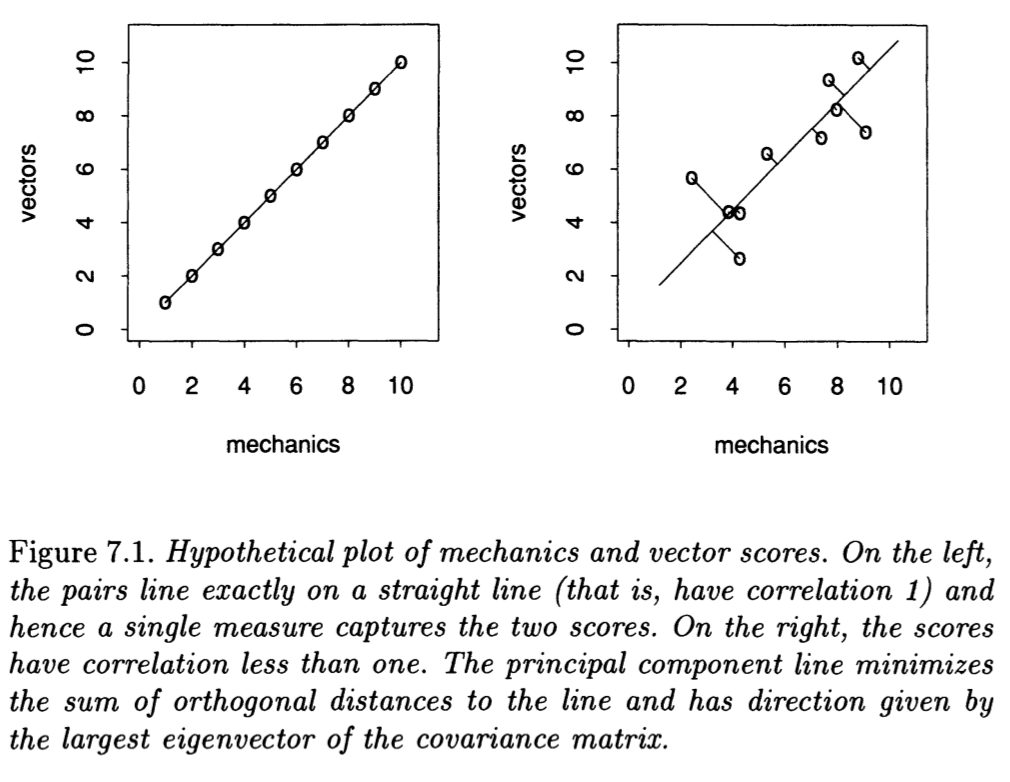
\includegraphics[width=0.85\linewidth]{6/f71.png}
\setcounter{figure}{1}

Во многих ситуациях такое большое значение $\hat \theta$ можно считать достаточно любопытным, что показывает высокую степень предсказательной силы модели (7.7).
Значение $\hat \theta$ измеряет процент дисперсии, объясняемой первой главной компонентой. Чем ближе точки лежат к прямой первой главной компоненты, тем выше значение $\hat \theta$.
Насколько точна оценка $\hat \theta$? Именно для ответа на такие вопросы бутстреп и был создан. Математическая сложность вычисления $\hat \theta$ не важна до тех пор пока мы можем подсчитать $\hat \theta^*$ для любых бутстреп данных. В этом случае бутстреп выборка представлена $\mathbf X^*$ --- матрицей $88\times 5$. Строки $\mathbf x_i^*$ матрицы $\mathbf X^*$ есть случайная выборка размера 88 из столбцов оригинальной матрицы $\mathbf X$
\begin{equation}
	\mathbf x_1^* = \mathbf x_{i_1}^*,\,\mathbf x_2^* = \mathbf x_{i_2}^*, \ldots,\, \mathbf x_{88}^* = \mathbf x_{i_{88}}^*, 
\end{equation}
как в (6.4). Некоторые строки матрицы $\mathbf X$ не появляются ни разу, некоторые один раз, некоторые дважды, и т.д., в итоге имеется 88 строк.

Сгенерировав матрицу $\mathbf X^*$, мы считаем её ковариационную матрицу $\mathbf G^*$ по аналогии с (7.4)
\begin{equation}
G_{jk}^* = \frac{1}{88}\sum_{i = 1}^{88} (x_{ij}^* - \bar x_j^*) (x_{ik}^* - \bar x_k^*), \qquad j,k = 1,2,3,4,5.
\end{equation}

Затем вычисляем собственные значения матрицы $\mathbf G^*$ --- $\hat \lambda_1^*, \hat \lambda_2^*,\ldots,\hat \lambda_5^* $ --- и в конце
\begin{equation}
	\hat \theta^* = \hat \lambda_1^* / \sum_{i = 1}^5 \hat \lambda_i^*,
\end{equation}
На рисунке 7.2 изображена гистограмма $B = 200$ репликаций бутстреп оценок $\hat \theta^*$. 
\newline
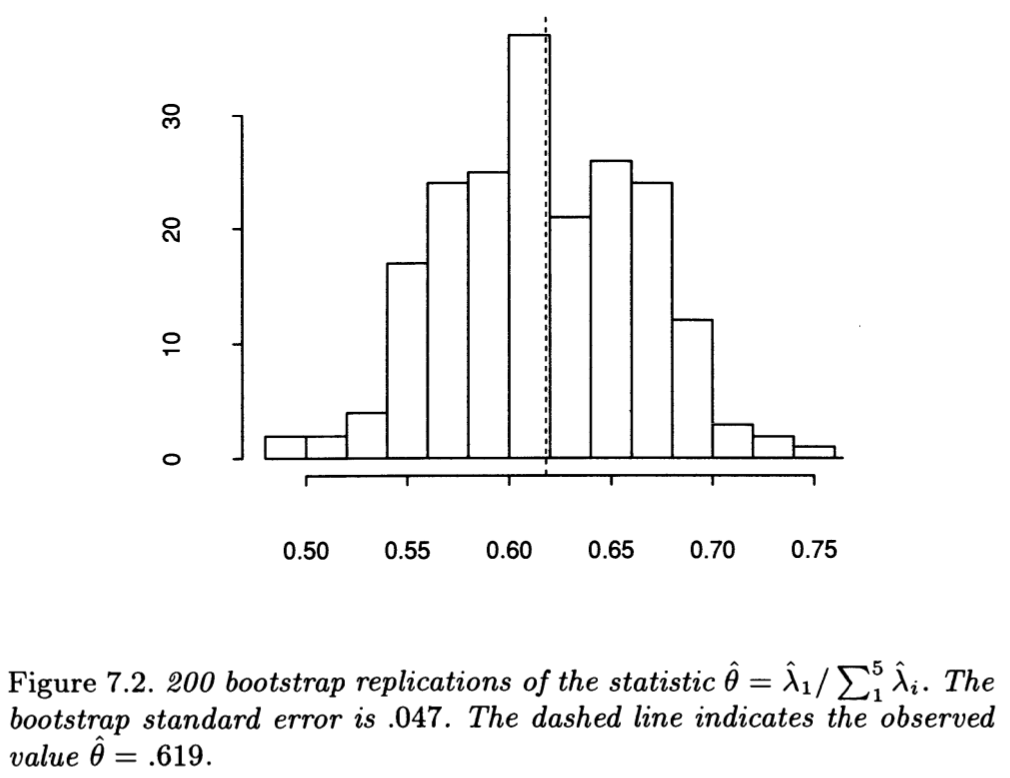
\includegraphics[width=0.85\linewidth]{6/f72.png}
\newline
\setcounter{figure}{2}

Они дают следующую оценку стандартной ошибки $\hat \theta^*$: $\widehat{\text{se}} = 0.047$. Среднее для всех 200 репликаций составило $0.625$, что лишь немногим больше, чем $\hat \theta = 0.619.$ Это означает, что $\hat \theta$ близка к несмещённой. Гистограмма выглядит адекватно, но $B = 200$ всё же недостаточно для того, чтобы ясно увидеть форму распределения. Некоторые квантили эмпирического распределения $\hat \theta^*$ показаны в таблице 7.2.

\noindent
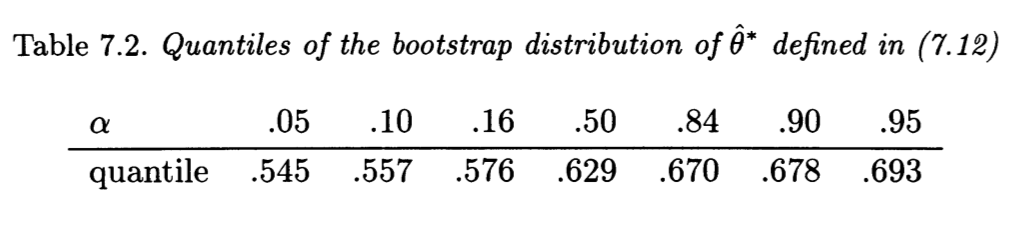
\includegraphics[width=0.9\linewidth]{6/t72.png}
\newline
\setcounter{table}{2}

\textit{Стандартный доверительный интервал} для настоящего значения $\theta$ (значениe $\hat \theta$, если устремить $n \rightarrow \infty$)
\begin{equation}
  \theta \in \hat \theta \pm z^{(1-\alpha)} \cdot \widehat{\text{se}} \qquad \text{(с вероятностью $1 - 2\alpha$)}
\end{equation}
где $z^{(1-\alpha)}$ есть $100(1- \alpha)$ персентиль стандартного нормального распределения; $z^{(.975)} = 1.960,z^{(.95)} = 1.645,z^{(.841)} = 1.000$, и т.д. Вычисление интервала основано на применении асимптотической теории, которая распространяет (5.6) на генеральные статистики $\hat \theta$. В нашем случае 
$$
\theta \in 0.619 \pm 0.047 = [ 0.572,0.666]\quad \text{с вероятностью }  0.683 
$$

$$
\theta \in 0.619 \pm 0.077 = [ 0.542,0.696]\quad \text{с вероятностью }  0.900. 
$$

В 12--14 главах обсуждаются улучшенные бутстреп доверительные интервалы, менее зависимые от асимптотической теории нормального распределения.

Случайный вектор $\hat{\mathbf v}_1$, относящийся к первому собственному значению, называется первой главной компонентой $\mathbf G$. Предположим, что мы хотим выразить результаты студента одним числом, а не пятью (например, для некоторого общего оценивания). Можно показать, что наилучшая линейная комбинация оценок есть 
\begin{equation}
  y_i = \sum_{k=1}^5 \hat{v}_{1k} x_{ik},
\end{equation}
то есть линейная комбинация, использующая компоненты $\hbv_1$ как веса. Эта линейная комбинация --- <<наилучшая>> в смысле того, что среди всех возможных $\mathbf v$ она отражает наибольшую вариативность в данных по пяти оценкам. Если же мы хотим описать успеваемость студента двумя числями, например $(y_i,z_i)$, вторая линейная комбинация должна выглядеть так

\begin{equation}
  y_i = \sum_{k=1}^5 \hat{v}_{2k} x_{ik},
\end{equation}
где веса взяты из второй главной компоненты $\hbv_2$, второго собственного значения матрицы $\mathbf G$.

Веса, заданные главными компонентами, часто дают понимание структуры многомерного набора данных. Для данных с оценками интерпретация будет следующей: первая главная компонента $$\hbv_1 = (0.51, 0.37, 0.35, 0.45, 0.54)$$ накладывает положительные веса примерно одинакового размера на каждый из тестов, то есть $y_i$ условно эквивалентно взятию суммарной (или средней) оценки $i$-го студента. Вторая главная компонента $$\hbv_2 = (-0.75, -0.2, 0.08, 0.30, 0.55)$$ даёт отрицательные веса двум тестам без использования конспекта и положительные на три теста с использованием конспекта, так что $z_i$ есть показатель \textit{разницы} оценок между тестами с открытым и закрытым конспектом для $i$-го студента. (Студент с высокой оценкой $z$ гораздо лучше справился с тестами с открытым конспектом, чем с закрытым.)

Векторы главных компонент $\hbv_1$ и $\hbv_2$ есть суммарные статистики, как и $\thetahat$, несмотря на то, что у каждой из них есть несколько компонент. Мы можем применить бутстреп анализ для того, чтобы узнать, насколько они устойчивы. Те же 200 бутстреп выборок, с помощью которых мы получили $\thetahat^*$, дают бутстреп репликации $\hbv_1^*$ и $\hbv_2^*$. Они могут быть посчитаны как первые два собственных вектора $\mathbf G^*$, (7.11).

В таблице 7.3 показаны $\seh_{200}$ для каждой из компонент векторов $\hbv_1$ и $\hbv_2$. Первое, что можно заметить --- это более высокую точность $\hbv_1$; бутстреп стандартная ошибка компонент $\hbv_1$ составляет менее половины ошибки $\hbv_2$. В таблице 7.3 также указаны основанные на персентилях робастные бутстреп стандартные ошибки $\sew_{200,\alpha}$, посчитанные для $\alpha = 0.84, 0.9, 0.95$. Для компонент $\hbv_1$ $\sew_{200, \alpha}$ примерно равно $\seh_{200}$. 
\\~\\
\noindent
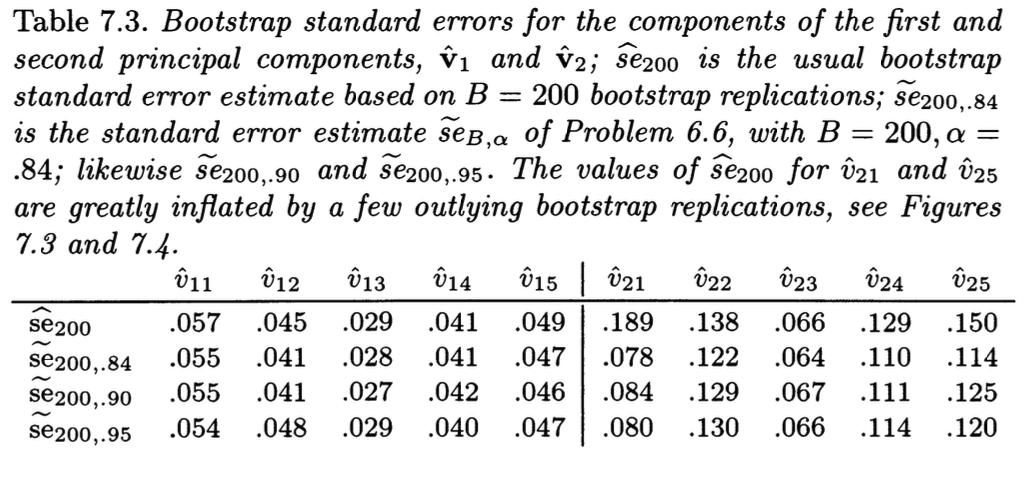
\includegraphics[width=0.9\linewidth]{6/t73.png}
\newline
\setcounter{table}{3}
Это не так для $\hbv_2$, в особенности для первой и пятой координаты. На рисунке 7.3 можно увидеть, в чём проблема. На рисунке показаны эмпирические распределения для 200 бутстреп репликаций $\hat v_{ik}^*$, в отдельности для каждого из $i = 1,2,\, k = 1,2,\ldots, 5$. Эмпирические распределения отражены ящиками с усами. Отрезок в центре ящика --- медиана распределения; нижняя и верхняя сторона ящика есть есть соответственно 25-я и 75-я персентиль распределения; усы покрывают всё распределение за исключением некоторых выбросов (определённых по некоторому критерию), которые отмечены звёздочкой.
\\~\\
\noindent
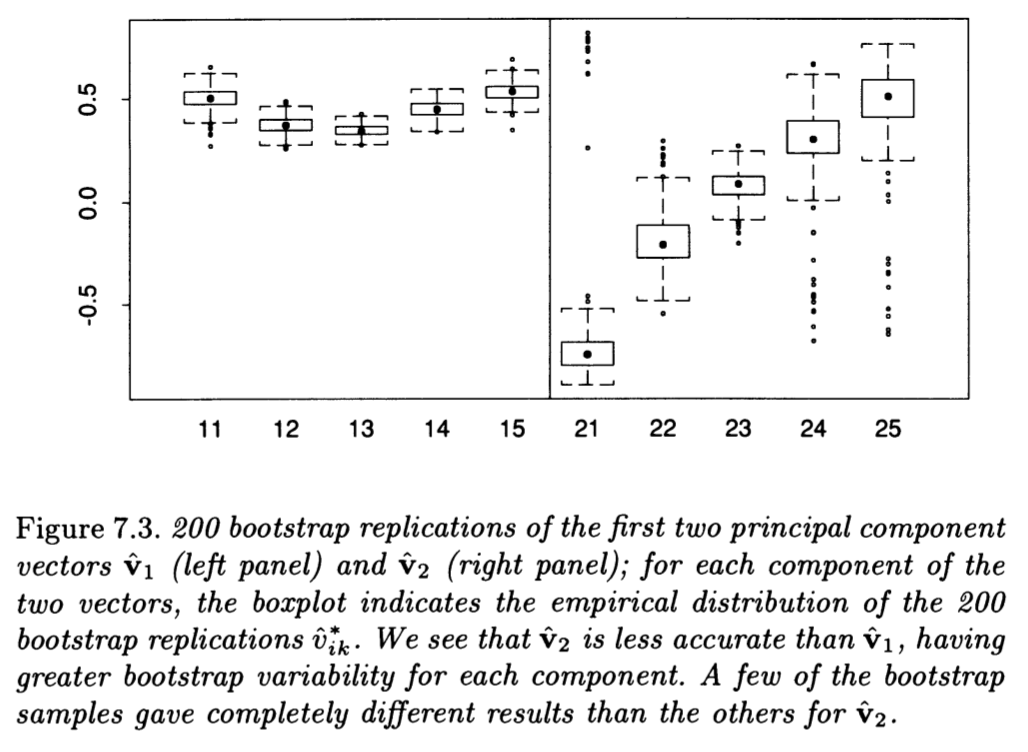
\includegraphics[width=0.9\linewidth]{6/f73.png}
\newline
\setcounter{figure}{3}

Можно увидеть, что большие значения $\seh_{200}$ для $\hat v_{21}$ и $\hat v_{25}$ вызваны несколькими выделяющимися значениями $\hat v_{ik}^*$. Приближённый доверительный интервал $\theta \in \thetahat \pm z^{1-\alpha} \seh$ будет более точным, если выбрать $\sew_{200, \alpha}$ в качестве оценки $\seh$, как минимум для умеренных значений $\alpha$ таких, как $0.843$. Гистограмма значений  $v^*_{21}$ имеет форму нормального распределения со средним в точке $-0.74$ и стандартным отклонением $0.075,$ с небольшим числом точек далеко от гистограммы. Это показатель того, что с малой вероятностью, порядка $1\%$ или $2\%$, что $\hat v_{21}$ оказывается совершенно неточной оценкой настоящего значения $v_{21}$. Если же данное событие не произошло, $\hat v_{21}$ вероятно находится в пределе одного или двух $\sew_{200}$ от $v_{21}$.

На рисунке 7.4 показаны графики бутстреп репликаций $$
\hbv_1^*(b)\tx{ и } \hbv_2^*(b),\qquad b=1,2,\ldots, 200,
$$ 
соединяющие компоненты каждого вектора прямыми. Это более наглядный (хоть и менее точный) показатель вариативности $\hbv_2$, чем предложенные ранее в таблице 7.3 и на рисунке 7.3.
Три конкретных репликации, отмеченные числами 1, 2, и 3, являются выбросами на нескольких компонентах.
\\~\\
\noindent
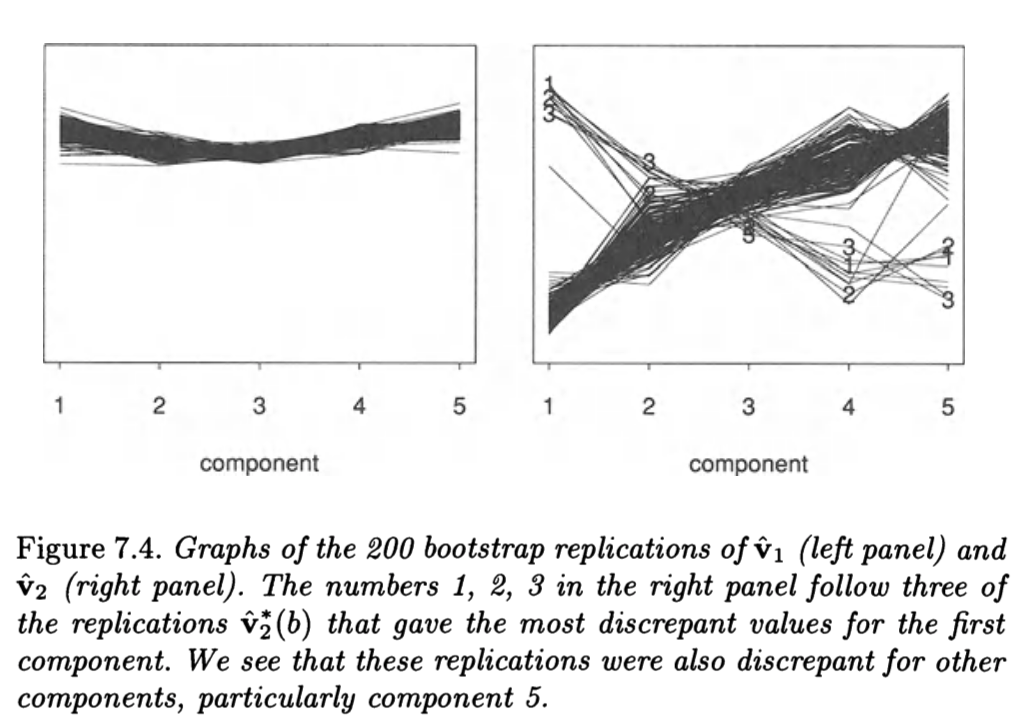
\includegraphics[width=0.9\linewidth]{6/f74.png}
\newline
\setcounter{figure}{4}

Читатель, которому знаком метод главных компонент, может теперь увидеть, что сложности со вторым собственным вектором объясняются проблемой единственности собственных векторов.
Технически, определение собственного вектора $\mathbf v$ также верно и для обратного ему вектора $- \mathbf v$. Алгоритм, который считает собственные числа и собственные значения, может приводить решения с разными знаками у $\hbv_1,\hbv_2,\ldots$ Репликации 1 и 2 привели к матрицам $\X^*$, для которых знак $\hbv_2^*$ получился обратным. Такая неопределённость обычно не важна при определении статистических особенностей оценок (хотя хорошо замечать такую неопределённость на основании результата применения бутстрепа). Если перестать учитывать 1 и 2, как происходит при оценке $\sew_{200,\alpha}$, мы видим, что $\hbv_2$ всё равно менее точна, чем $\hbv_1$.






\section{Пример 2: построение кривой по данным}

В этом примере мы будем оценивать функцию регрессии двумя способами, сначала с помощью стандартного метода наименьших квадратов, а затем с помощью современного метода построения кривой по данным, который называется \textit{loess}. Мы начнём с краткого повторения теории регрессии. В главе 9 снова рассматривается задача регрессии и дан альтернативный бутстреп метод для оценки стандартных ошибок регрессии. На рисунке 7.5 показан типичный набор данных, для которого используются регрессионные методы:  мужчин приняли участие в эксперименте, чтобы определить, уменьшает ли лекарство на основе холостирамина уровень холестерина в крови. Мужчины должны были принимать по 6 пакетиков холостирамина в день, однако многие из них принимали гораздо меньше.
\\~\\
\noindent
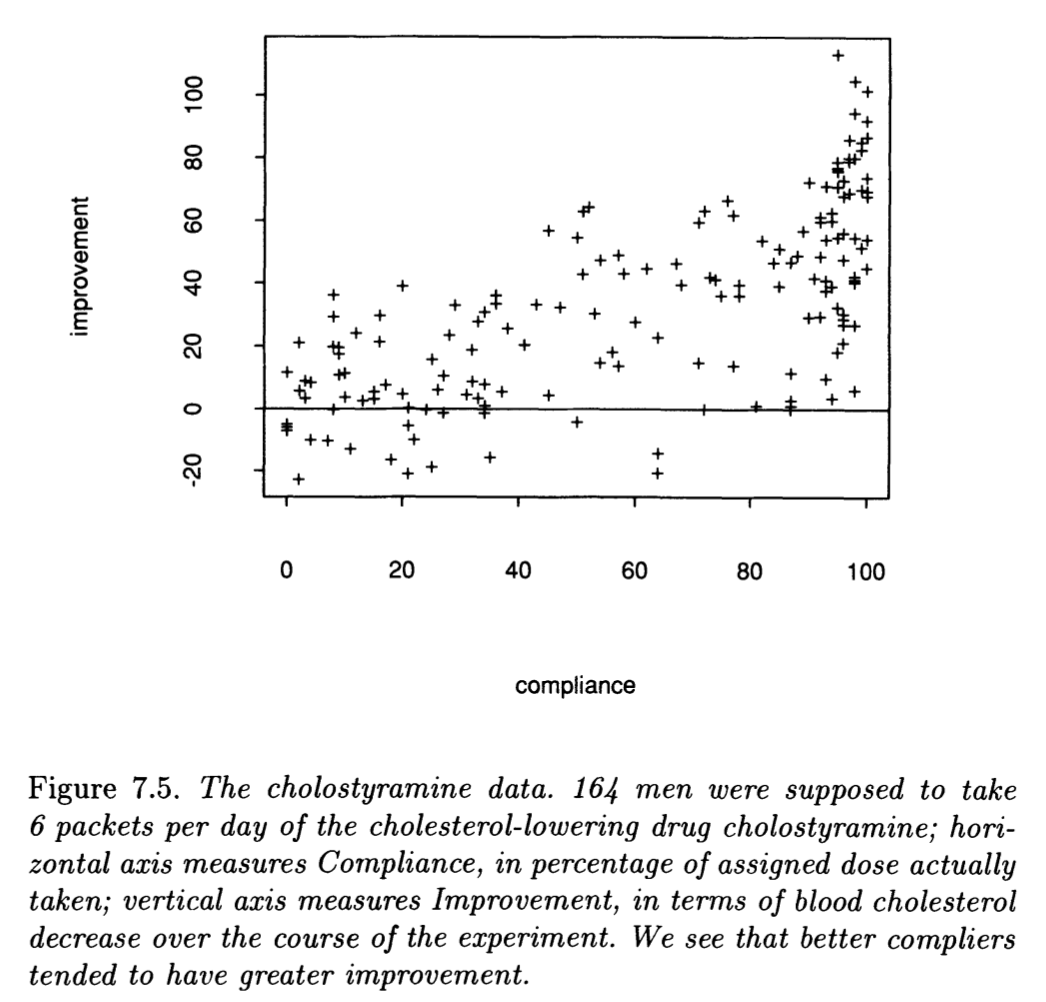
\includegraphics[width=0.9\linewidth]{6/f75.png}
\newline
\setcounter{figure}{1}

Горизонтальная ось, которую мы назовём <<$z$>>, измеряет <<Соответствие>>, то есть процент приёма от назначенной дозы,
$$
z_i = \text{ процент соответствия для мужчины } i,\, i = 1,2,\ldots, 164.
$$

Соответствие измерялось подсчётом количества пакетиков, которые вернули индивиды. Те, кто приняли все пакетики, находятся в правом краю графика; те, кто не принимал ничего --- в левом. Горизонтальная ось, отмеченная <<$y$>>, есть показатель \textit{Улучшения}, уменьшение уровня холестерина в кровяной плазме за время исследования,
$$
y_i = \text{ уменьшение уроня холестерина в крови для индивида } i,\, i = 1,2,\ldots, 164.
$$
Полный набор данных представлен в таблице 7.4.
\\~\\
\noindent
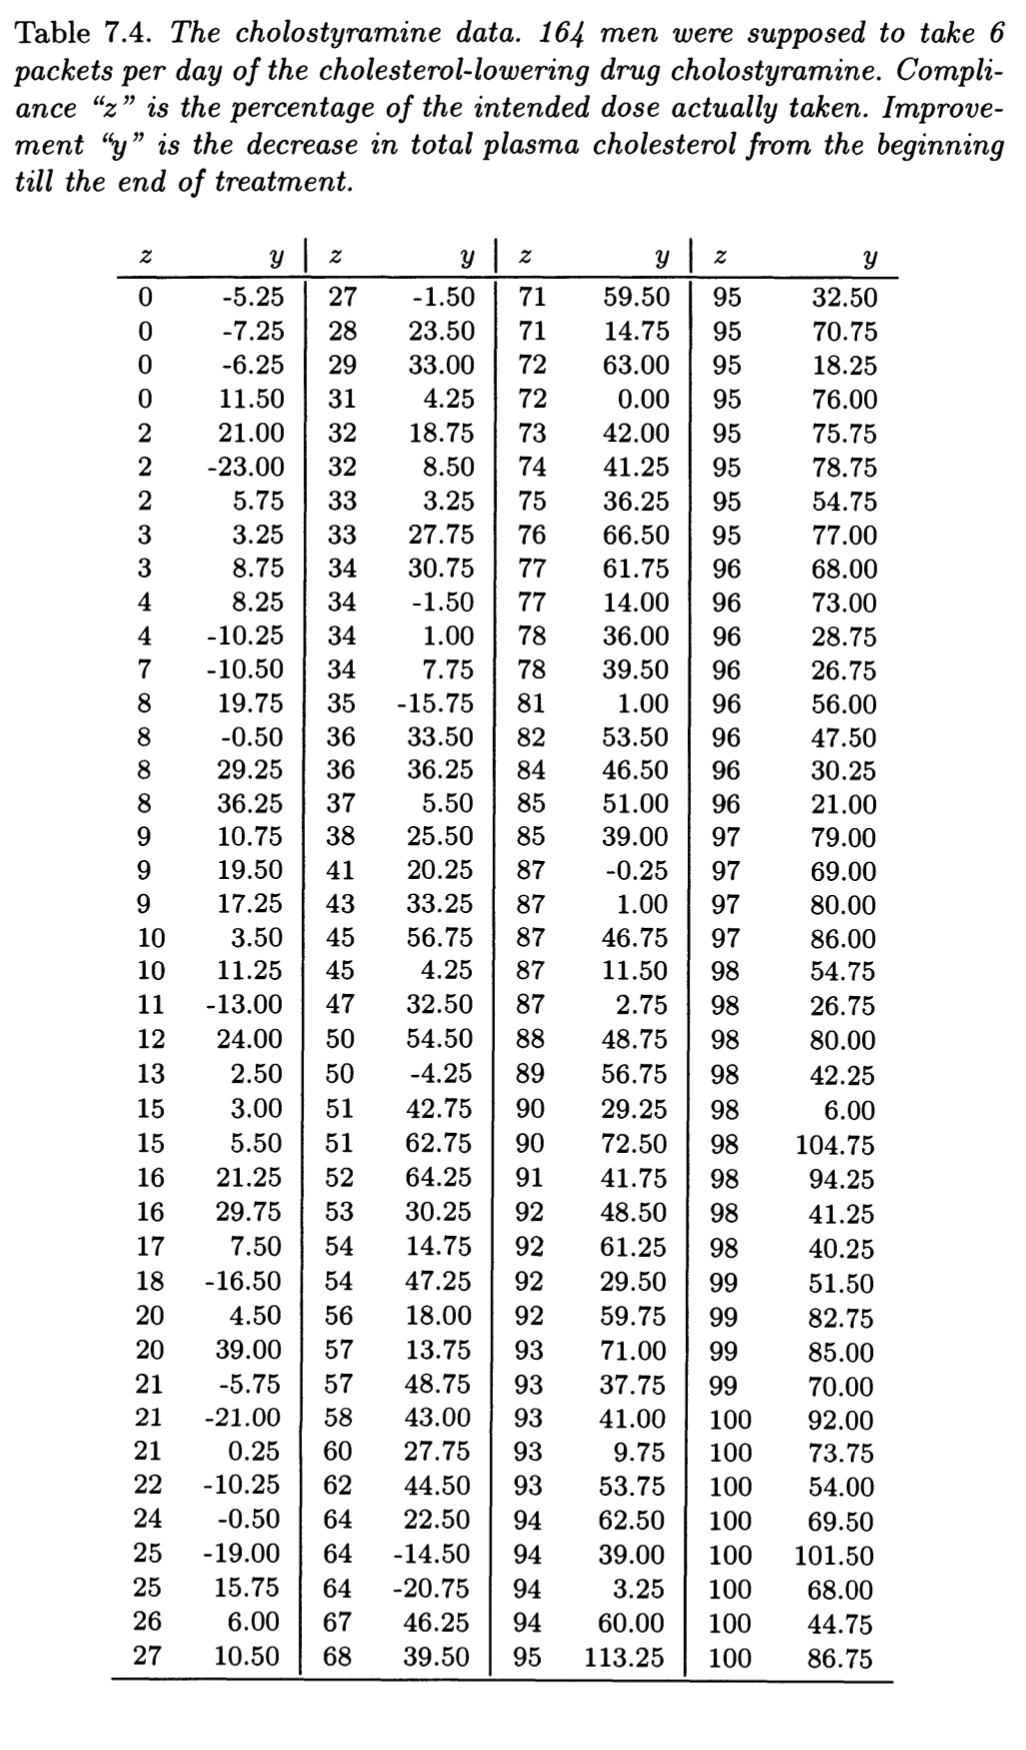
\includegraphics[width=0.95\linewidth]{6/t74.png}
\newline
\setcounter{table}{4}

 На рисунке видно, что мужчины, которые принимали больше хлоростирамина, в целом улучшили свои показатели холестерина, что и ожидалось. То, что мы видим на рисунке 7.5, или скорее то, что мы хотели бы видеть, есть увеличение среднего ответа $y$ в то время как $z$ увеличивается от 0 до $100\%$. На рисунке 7.6 показаны данные вместе с двумя графиками,
\begin{equation}
\hat r_\text{quad}(z) \text{ и }  \hat r_\text{loess}(z).
\end{equation}
\\~\\
\noindent
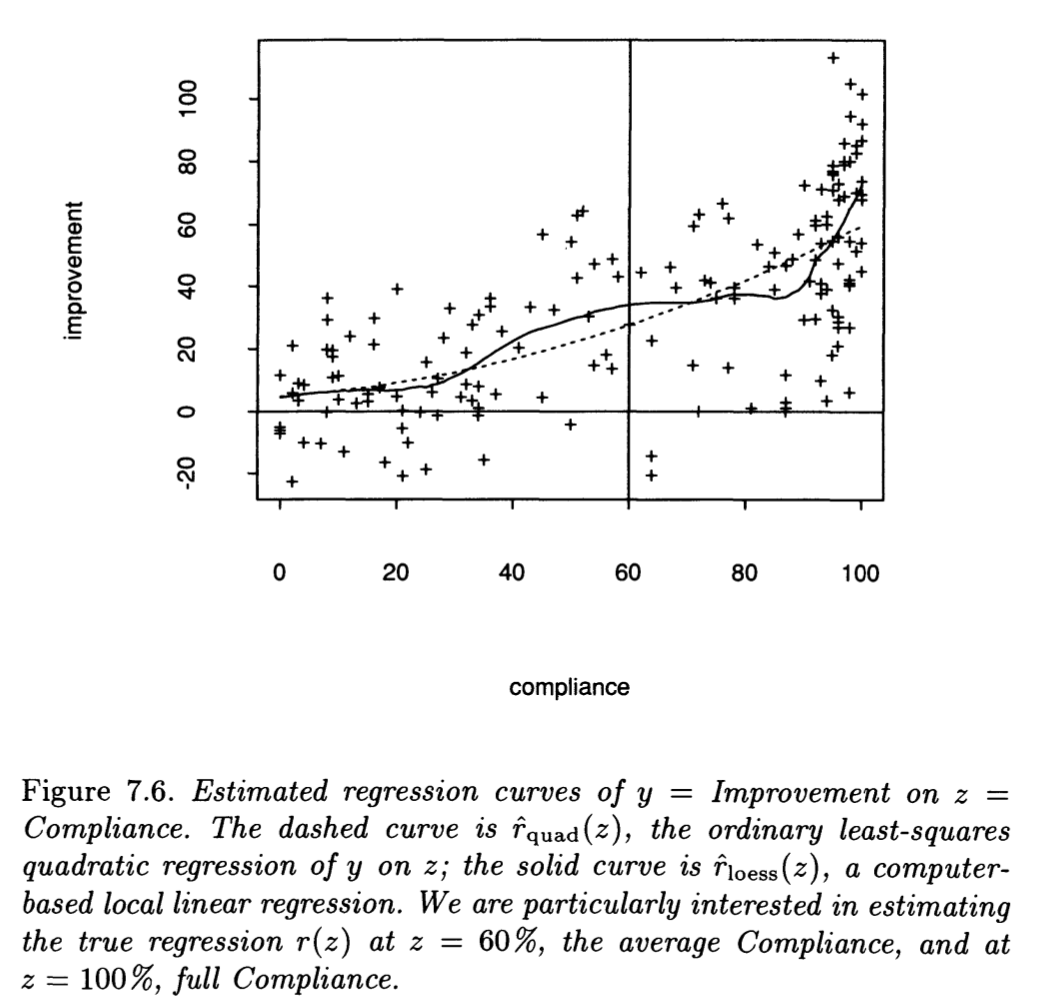
\includegraphics[width=0.9\linewidth]{6/f76.png}
\newline
\setcounter{figure}{7}

Каждый из них есть оценка кривой регрессии. Сейчас будет краткое повторение построения и оценки регрессионных кривых.
По определению регрессией ответа $y$ на независимую переменную $z$ называется условное математическое ожидание $y$ при некотором $z$,
\begin{equation}
  r(z) = \mathrm E(y|z).
\end{equation}
Предположим, что нам была доступна вся популяция $\mathcal U$ мужчин, подходящих для эксперимента, и мы получили набор $\mathcal X = (X_1,X_2,\ldots, X_N)$ оценок \textit{Соответствие-улучшение} $X_j = (Z_j, Y_j),\, j = 1,2,\ldots,N.$ Далее для каждого значения $z$, например $z = 0\%,1\%,2\%,\ldots,100\%$, регрессия была бы условным математическим ожиданием (7.17),
\begin{equation}
  r(z) = \frac{\text{сумма значений $Y_j$ для мужчин в $\mathcal X$ с $Z_j = z$}}{\text{число мужчин в $\mathcal X$ с $Z_j = z$}}.
\end{equation}
 Другими словами, $r(z)$ есть математическое ожидание $Y$ для субпопуляции мужчин, у которых $Z= z$.
 
 Разумеется у нас нет целой популяции $\mathcal X$. У нас имеется выборка $\mathbf x = (\mathbf x_1, \mathbf x_2, \ldots, \mathbf x_{164})$, где $\mathbf x_i = (z_i, y_i)$, как показано на рисунке 7.5 и в таблице 7.4. Как мы можем оценить $r(z)$? Очевидная оценка методом подстановки есть
 \begin{equation}
  \hat r(z) = \frac{\text{сумма значений $y_j$ для мужчин в $\mathbf x$ с $z_j = z$}}{\text{число мужчин в $\mathbf x$ с $z_j = z$}}.
\end{equation}

Можно представить себе разбиение на вертикальные полосы шириной в $1\%$ на рисунке 7.5 и усреднение значений на каждой полосе для получения $\hat r(z).$ Результаты можно увидеть на рисунке 7.7.
\\~\\
\noindent
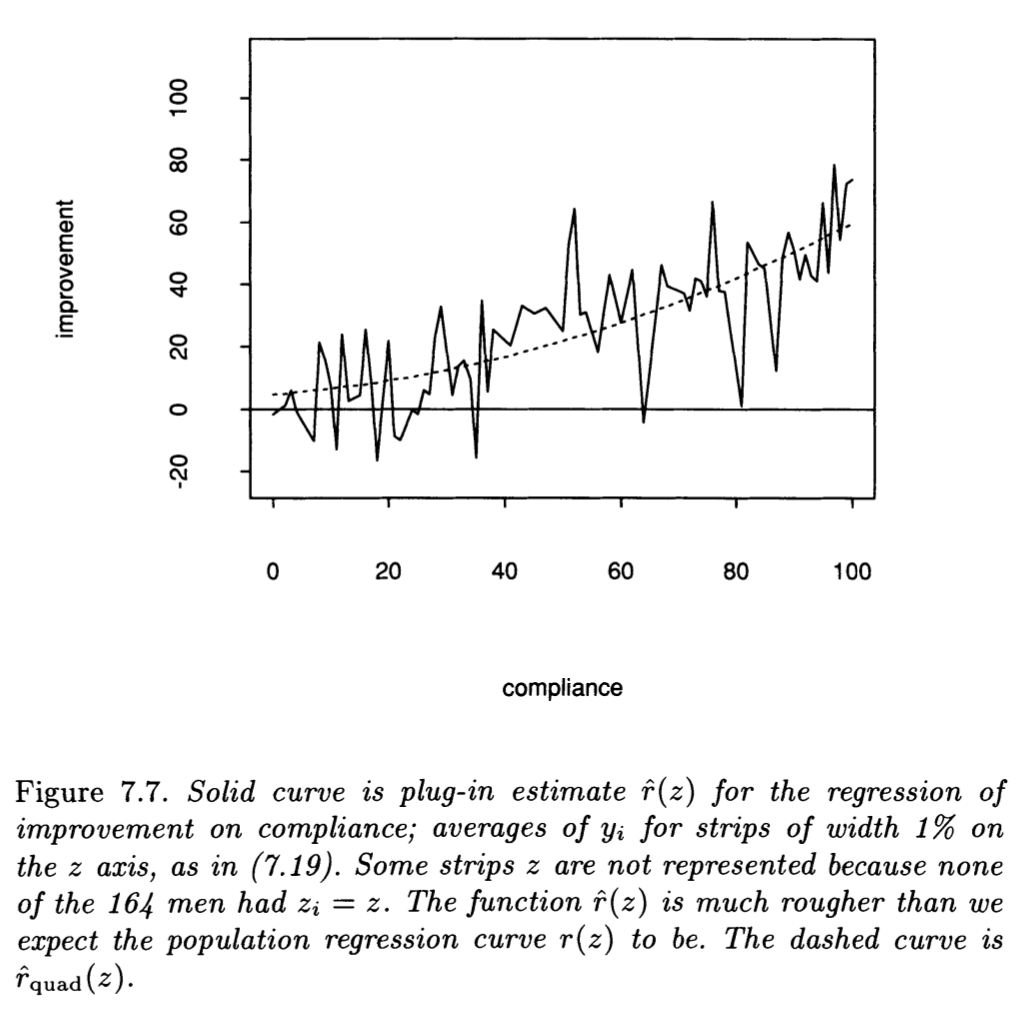
\includegraphics[width=0.9\linewidth]{6/f77.png}
\newline
\setcounter{figure}{7}

Впервые нашёлся пример, для которого метод подстановки работает не очень хорошо. Оценка регрессии $\hat r(z)$ гораздо грубее, чем мы хотели бы для оценки популяционной регрессии $r(z)$. Проблема в том, что внутри каждой полосы шириной в $1\%$ точек для адекватной оценки $r(z)$ недостаточно. Для некоторых полос шириной в $5\%$ точек внутри нет вообще. Мы можем увеличить ширину промежутка, скажем, до $10\%$ вместо $1\%$, но это не исправит проблему небольшого числа точек и, вероятно, проблема неустойчивости всё равно останется. На самом деле, имеется более элегантное и эффективное решение, которое основано на методе наименьших квадратов.

Использование метода начинается с предположения, что популяционная регрессионная функция, какая бы она не была, принадлежит семейству $\mathcal R$ гладких функций, индексированных вектором параметров $$\bm \beta = (\beta_0,\beta_1,\ldots,\beta_p)^\mathrm{T}$$. Для рассматриваемого примера мы ограничимся семейством квадратичных функций от $z$, скажем, $\mathcal R_\text{quad},$
\begin{equation}
  \mathcal R_\text{quad: \quad} r_{\bm \beta}(z) = \beta_0 + \beta_1 z + \beta_2 z^2,
\end{equation}
поэтому $\bm \beta = (\beta_0,\beta_1,\beta_2)^\mathrm{T}$. Далее мы обсудим выбор именно квадратичного семейства $\mathcal R_\text{quad},$ но на сейчас примем это как данное.

Читатель может представить себе выбор некоторого пробного значения $\bm \beta$, к примеру, $\bm \beta = (0,0.75,0.005)^\mathrm{T}$, и построение $r_\beta(z)$ на рисунке 7.5. Мы хотели бы, чтобы кривая $r_\beta(z)$ проходила близко к нашим данным $(z_i, y_i)$ в некотором общем смысле. Наиболее удобно для вычислений измерять близость кривой к данным с помощью суммы квадратов остатков (\textit{Residual Squared Error}),
\begin{equation}
  \rse(\bm \beta) = \sum_{i = 1}^n [y_i - r_{\bm \beta} (z_i)]^2.
\end{equation}
Сумма квадратов остатков получается опусканием вертикальных отрезков от каждой точки $(z_i, y_i)$ к кривой $r_{\bm \beta} (z_i)$, а затем суммированием квадратов их длин.

\textit{Метод наименьших квадратов}, созданные Гауссом и Лежандром в начале 19 века, выбирает среди кривых в $\mathcal R$ те, которые минимизируют $\rse$. Наилучший из них объявляется $r_{\hat {\bm \beta}}(z),$ где $\hat {\bm\beta}$ минимизирует $\rse(\bm \beta)$,
\begin{equation}
  \rse(\hat{\bm \beta}) = \min_{\bm \beta}{\rse(\bm \beta)}.
\end{equation}
 Кривая $\rquad(z)$ на рисунке 7.6 есть $r_{\hat{\bm \beta}}(z) = \hat \beta_0 + \hat \beta_1 z + \hat \beta_2 z^2,$ наилучшая квадратичная функция для наших данных.
 
 Лежандр и Гаусс обнаружили замечательную явную формулу для решения $\hat{\bm \beta}$ задачи наименьших квадратов. Пусть $\mathbf C$ есть матрица $164\times 3,$ $i$-я строка которой есть
 \begin{equation}
  \bm c_i = (1, z_i, z_i^2),
\end{equation}
и пусть $\mathbf y$ есть вектор из 164 значений $y_i.$ Тогда, используя стандартную матричную нотацию, имеем
\begin{equation}
  \hat{\bm \beta} = (\mathbf C^\mathrm{T} \mathbf{C})^{-1} \mathbf{C}^\mathrm{T} \mathbf y.
\end{equation}
Более  подробно мы рассмотрим эту формулу в главе 9. Для наших целей, связанных с применением бутстрепа, нам достаточно лишь знать про то, что набор данных из $n$ пар $\mathbf x = (\mathbf x_1, \mathbf x_2,\ldots, \mathbf x_n)$ приводит к получению квадратичной кривой $r_{\hat{\bm \beta}}(z)$ через отображение $\mathbf x \rightarrow r_{\hat{\bm \beta}}(z),$ которое описывается (7.23), (7.24) и (7.20).

Можно рассматривать $r_{\hat{\bm \beta}}(z)$ как сглаженную версию оценки по методу подстановки $\hat r(z)$. Предположим, что мы бы рассмотрели более широкий класс гладких функций $\mathcal R,$ к примеру, класс кубических функций $\mathcal R_\text{cubic}.$ В таком случае решение по методу наименьших квадратов $r_{{\hat{\bm\beta}}}(z)$ стало бы ближе к данным, однако оказалось бы более <<бугристым>>, чем квадратичное решение по методу наименьших квадратов. Если бы мы начали рассматривать полиномы всё большей степени, $r_{\hat{\bm \beta}}$ всё больше бы походил на оценку по методу подстановки $\hat r  (z)$. Выбор семейства квадратичных функций основан на нашем представлении о том, насколько гладкой должна быть оригинальная функция регрессии $r(z)$.
 Смотря на рисунок 7.7, мы явно видим, что $\rquad(z)$ гораздо более гладкая, чем $\hat r (z),$ однако в целом соответствует $\hat r (z)$ как функция от $z$.
 
Легко поверить, что настоящая функция регрессии $r(z)$ есть гладкая функция от $z$.  Сложнее поверить в то, что $r(z)$ является квадратичной от $z$ для всех значений $z$. Сглаживающая функция \textit{loess} является компромиссом между \textit{глобальными} предположениями о форме и чисто \textit{локальным} усреднением $\hat r(z)$.  

Для использования loess нужно указать число $\alpha$, которое равно части $n$ точек, используемых при построении кривой в каждой из точек. Кривая $\rloess (z)$ на рисунке 7.6 построена при выборе $\alpha = 0.3$. Для каждого из значений $z$ значение $\rloess (z)$ получается следующим образом:
\begin{enumerate}
	\item $n$ точек $\mathbf x_i = (z_i, y_i)$  упорядочиваются согласно $|z_i - z|,$ а ближайшие $\alpha \cdot n$ точек с наименьшим $|z_i - z|$, запоминаются. Назовём эти точки $\mathcal N(z)$.\footnote{при выборе $\alpha= 0.3, n=164$, алгоритм выбирает в $\mathcal N(z)$ 49 точек}
	\item Взвешенная линейная регрессия (с минимизацией наименьших квадратов) 
	\begin{equation}
  	\hat r_z(Z) = \hat \beta_{z,0} + \hat \beta_{z,1} Z
	\end{equation}
	производится для $\alpha \cdot n$ точек в $\mathcal N(z)$. [То есть коэффициенты $ \hat \beta_{z,0}$ и $\hat \beta_{z,1}$ выбираются как минимизирующие $\sum_{\mathbf x_j \in \mathcal N} w_{z,j} [y_j - (\beta_0 + \beta_1 z_j)]^2$, где веса $w_{z,j}$ есть положительные числа, зависящие от $|z_j - z|$. Взяв 
	\begin{equation}
  u_j = \frac{|z_j - z|}{\max_{\mathcal N (z)}|z_k - z|},
\end{equation}
веса $w_j$ выбираются равными $(1 - u_j^3)^3$.]

	\item В итоге, $\rloess (z)$ назначается равным числу $\hat r_z(Z)$ в точке $Z = z,$
\begin{equation}
  \rloess(z) = \hat r_z (Z=z).
\end{equation}
\end{enumerate}
~\\
\noindent
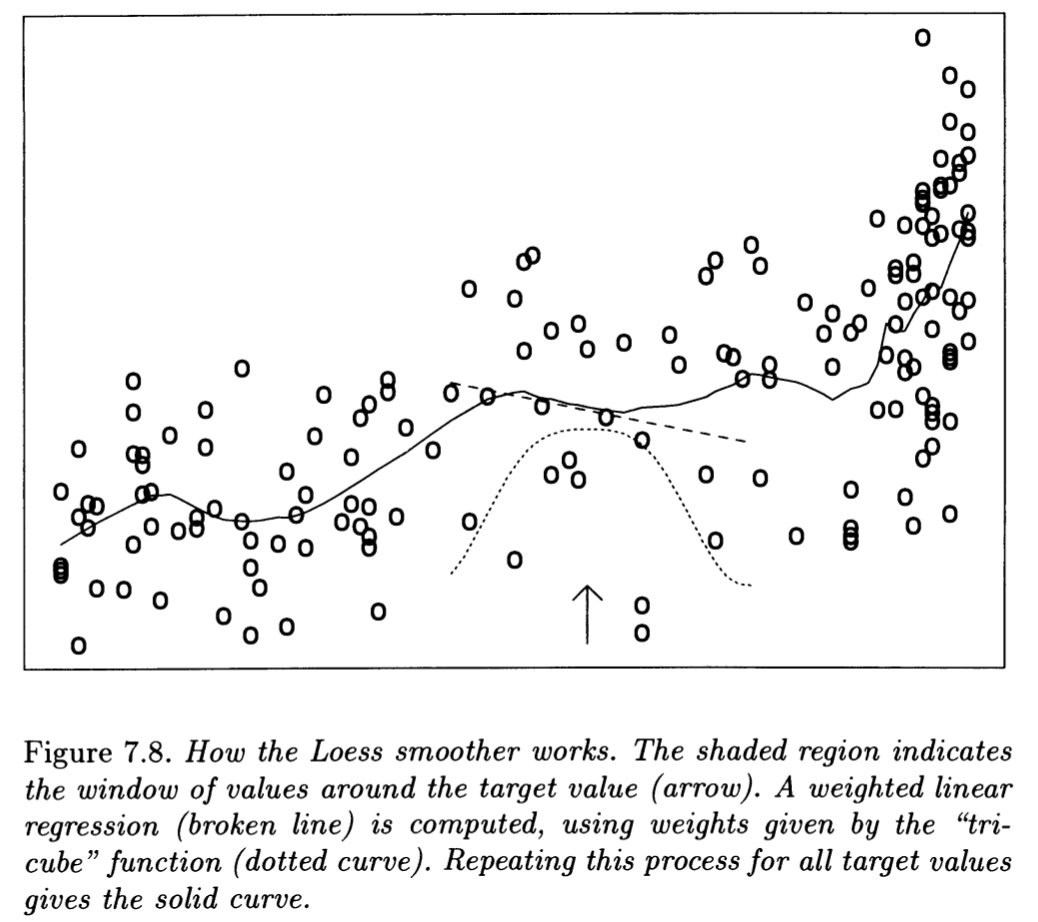
\includegraphics[width=0.9\linewidth]{6/f78.png}
\newline
\setcounter{figure}{8}

Компоненты loess сглаживания показаны на рисунке 7.8. В таблице 7.5 показано сравнение $\rquad(z)$ и $\rloess(z)$ в двух значениях, представляющих наибольший интерес, $z = 60\%$ и $z = 100\%$. Стандартные ошибки по бутстрепу даны для каждого из значений. Они были получены из $B = 50$ бутстреп репликаций алгоритма, показанного на рисунке 6.1.
\\~\\
\noindent
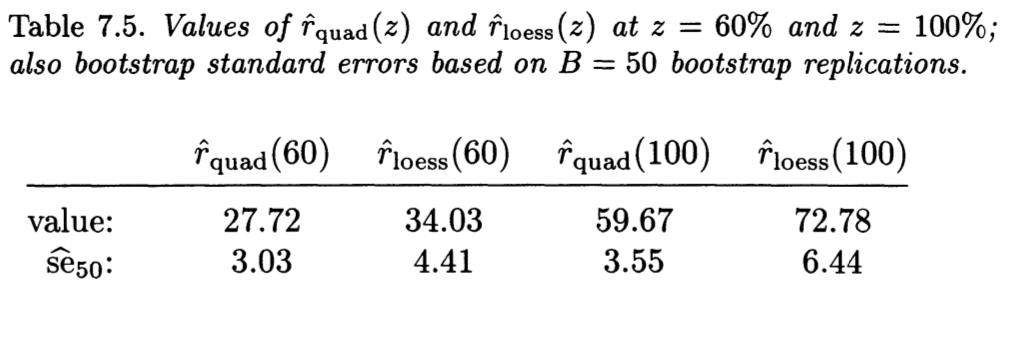
\includegraphics[width=0.9\linewidth]{6/t75.png}
\newline
\setcounter{table}{5}

В данном случае $\hat F$ есть распределение, дающее вероятность $1/164$ каждому из 164 наблюдений $\mathbf x_i = (z_i, y_i).$ Бутстреп набор есть $\mathbf x^* = (\mathbf x_1^*,\mathbf x_2^*, \ldots, \mathbf x_{164}^*),$ где каждый из $\mathbf x_i^* $ равен одному из 164 наблюдений с одинаковой вероятностью. Получив $\mathbf x^*,$ мы вычислили $\rquad^*(z)$ и $\rloess^*(z)$, квадратичную и loess кривые на основе $\mathbf x^*.$ В завершение мы вычислили значения $\rquad^*(60)$ и $\rloess^*(60)$, а также $\rquad^*(100)$ и $\rloess^*(100)$. $B = 50$ значений $\rquad^*(60)$ имеют стандартную ошибку $3.03$ и т.д., см. таблицу 7.5.

Посмотрев на результаты в таблице 7.5, можно сделать вывод о том, что оценка $\rloess(z)$ значительно менее точна, чем $\rquad(z).$	Это неудивительно, ведь $\rloess(z)$ строится на меньшем количестве данных (размер обусловлен $\alpha$), чем $\rquad(z)$. Неустойчивость $\rloess(z)$ очевидна по графикам на рисунке 7.9.
\\~\\
\noindent
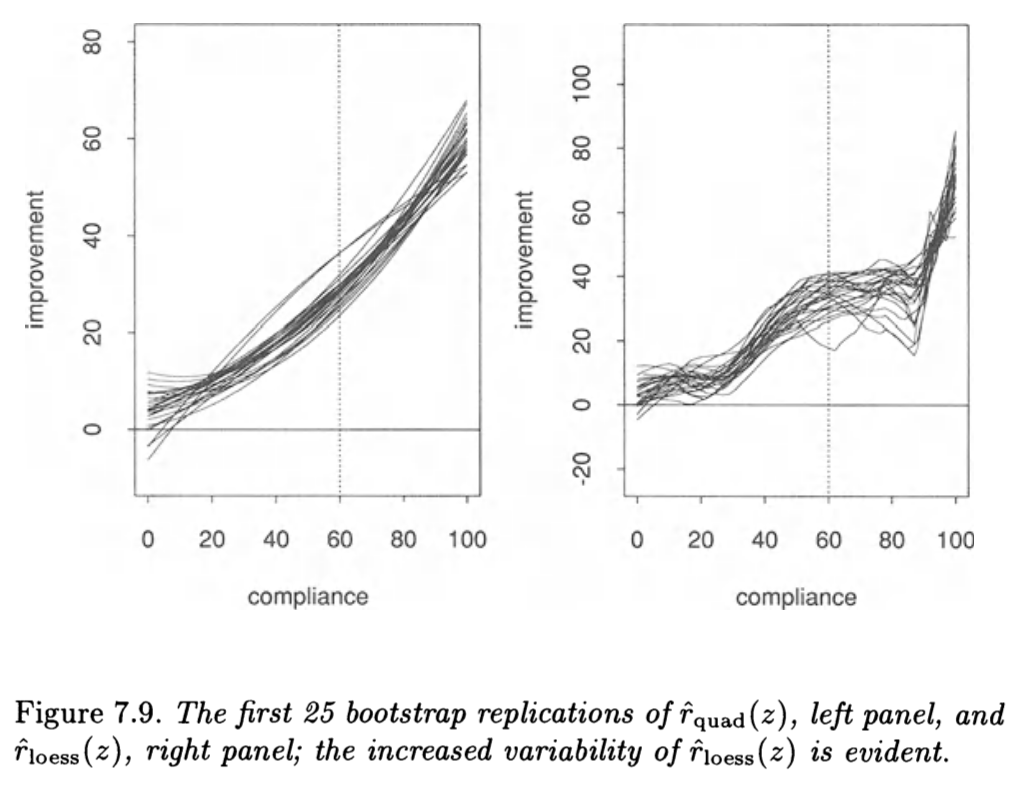
\includegraphics[width=0.9\linewidth]{6/f79.png}
\newline
\setcounter{figure}{9}

Полезно построить кривые бутстрепа, чтобы увидеть, сохраняются ли некоторые интересные особенности оригинальной кривой у кривых по бутстреп выборкам. Например, на рисунке 7.6 видим, что $\rloess(z)$ растёт гораздо быстрее с $z = 80\%$ до $z = 100\%$, чем с $z = 60\%$ до $z = 80\%$. Разность средних у углов наклона составляет
\begin{align}
	\thetahat &= \frac{\rloess(100) - \rloess(80)}{20} - \frac{\rloess(80) - \rloess(60)}{20}\nonumber \\
	&= \frac{672.78 - 37.50}{20} - \frac{32.50 - 34.03}{20} = 1.84.
\end{align}
  
Соответствующее число для $\rquad$ составляет лишь $0.17$. Большинство loess кривых показывают похожий быстрый рост примерно на $80\%$. Ни одно из бутстреп значений $\thetahat^*$ не было меньше нуля, минимум составил 0.23, большинство значений оказались больше единицы, см. рисунок 7.10.
\\~\\
\noindent
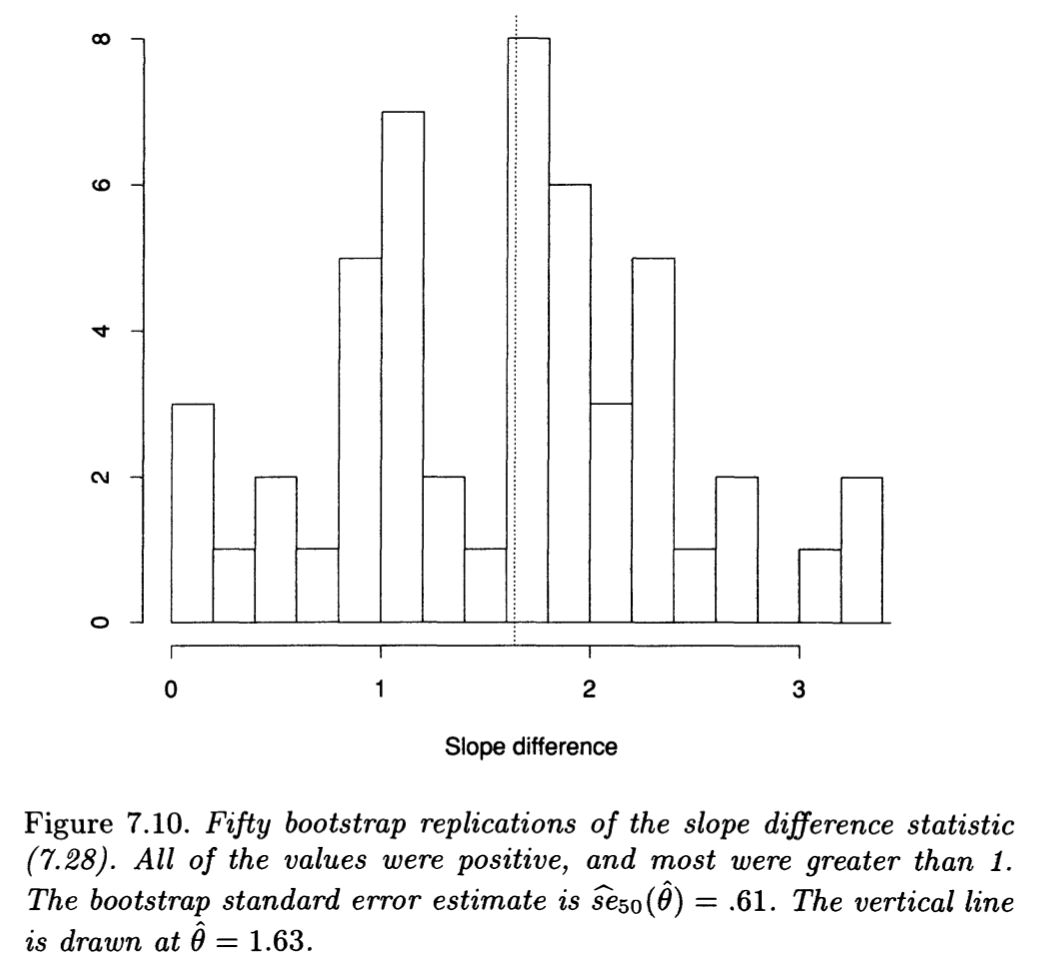
\includegraphics[width=0.9\linewidth]{6/f710.png}
\newline
\setcounter{figure}{10}
В такой момент мы можем законно опасаться того, что $\rquad(z)$ является \textit{слишком} гладкой оценкой оригинальной регрессионной функции $r(z)$. Если значение настоящей разности в углах наклона
\begin{equation}
  \theta = \frac{r(100) - r(80)}{20} - \frac{r(80) - r(60)}{20}
\end{equation}
и находится около $\thetahat = 1.59,$ то $r(z)$ будет выглядеть скорее как 
$\rloess(z)$, чем $\rquad(z)$ для $z$ между 60 и 100. Оценки, построенные на $\rloess(z)$ обычно отличаются высокой дисперсией, как в таблице 7.5, но в то же время имеют низкое смещение. Оба этих свойства происходят от локального характера алгоритма loess, который строит оценку $r(z)$ используя только элементы выборки в окрестности $z$.

Оценка $\thetahat = 1.59$, построенная на $\rloess$ имеет большую вариативность, $\seh_{50} = 0.61$, однако содержание рисунка 7.10 явно намекает на то, что настоящее значение $\theta$, каким бы оно ни было, больше, чем значение $\thetahat = 0.17,$ основанное на $\rquad.$ Мы рассмотрим эту проблему детальнее в главах 12--14 про бутстреп доверительные интервалы.

Таблица 7.5 намекает на то, что нам следует беспокоиться за оценки $\rquad(60)$ и $\rquad(100),$ которые могут быть значительно заниженными. Одним из возможных решений этой проблемы может быть выбор полиномиальных моделей более высокой размерности. Достаточно замысловатые теории построения моделей были предложены с целью определить, когда следует продолжать поиск модели в пространстве большей размерности, а когда следует остановиться. Мы глубже рассмотрим вопрос построения регрессионных моделей в главе 9, где данные примера 2 мы рассмотрим снова. Простые бутстреп оценки вариативности и неустойчивости, которые были освещены в данной главе, часто становятся полезным шагом в сторону понимания регрессионных моделей, в особенности нетрадиционных (таких как $\rloess(z)$).
\section{Пример отказа бутстрепа}

Предположим, что у нас имеются данные $X_1, X_2,\ldots, X_n$ из равномерного распределения на $(0, \theta)$. Оценка $\thetahat$ по методу максимума правдоподобия есть наибольшее значение выборки $X_{(n)}.$ Мы сгенерировали выборку из 50 равномерно распределённых чисел на $(0,1)$ и получили $\thetahat = 0.988.$ На левой части рисунка 7.11 показана гистограмма 2000 бутстреп репликаций оценки $\thetahat^*$, полученных с помощью выборок из данных с возвращением. На правой части наблюдаем 2000 репликаций параметрического бутстрепа, полученных при взятии выборок из равномерного распределения на $(0, \thetahat).$\footnote{подписи parametric и nonparametric на рисунке следует поменять местами --- прим.ред.} Ясно, что гистограмма слева есть плохая аппроксимация того, что мы видим на правой. Так, в случае левой гистограммы оказывается, что в $62\%$ репликаций $\thetahat^* = \thetahat$. Вообще говоря, легко показать, что $\text{Prob}(\thetahat^* = \thetahat) = 1 - (1 - 1/n)^n \rightarrow 1 - e^{-1} \approx .632$ когда $n \rightarrow \infty.$ Однако, в параметрическом случае правой гистограммы $\text{Prob}(\thetahat^* = \thetahat) = 0$.
\\~\\
\noindent
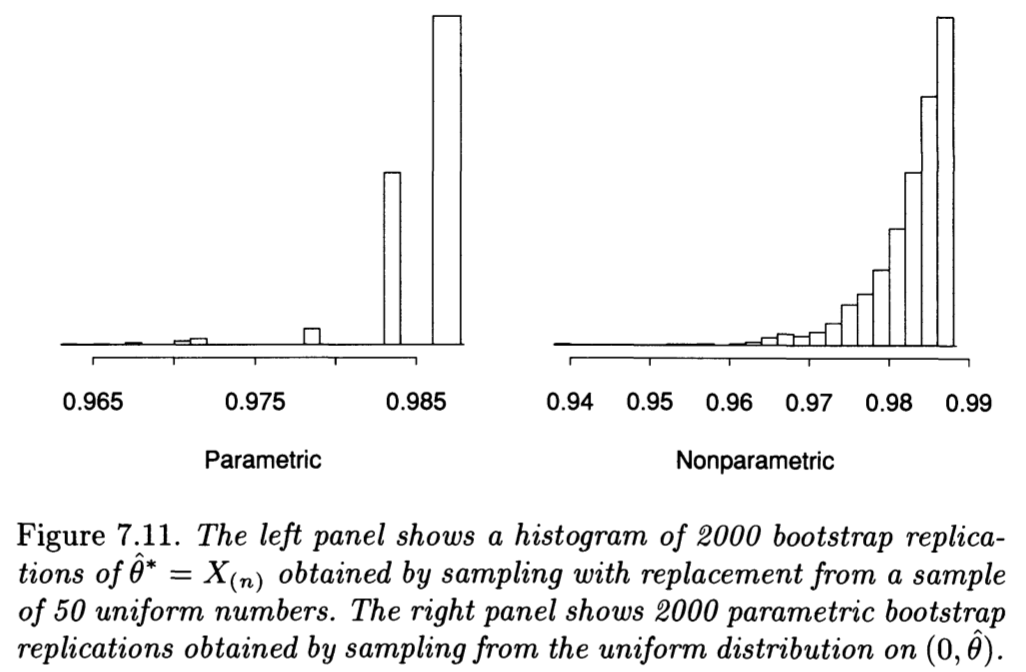
\includegraphics[width=0.9\linewidth]{6/f711.png}
\newline
\setcounter{table}{5} 
Что не так с непарамерическим бутстрепом? Сложность возникает потому, что эмпирическая функция распределения $\hat F$ не является хорошей оценкой настоящего распределения на его краях. Либо параметрические данные о $F$, либо некоторое сглаживание $\hat F$ необходимо для того, чтобы разрешить эту проблему. Детали и ссылки об этой проблеме можно найти в Beran и Ducharme (1991, с.23). Непараметрический бутстреп может отказать и в других примерах, где $\theta$ зависит от гладкости $F.$ К примеру, если $\theta$ есть число атомов у $F$, то $\thetahat = n$ будет плохой оценкой $\thetahat.$ 

\setcounter{chapter}{7}
\chapter{Более сложные структуры данных}
\section{Введение}

Алгоритм бутстрепа на рисунке 6.1 основан на простейшей возможной вероятностной модели для случайных данных: одновыборочная модель, в которой одно неизвестное вероятностное распределение $F$ порождает данные $\textbf{x}$ путем случайной выборки
\begin{equation}
	F \to \textbf{x} = (x_1, x_2, \ldots , x_n).
\end{equation}
Отдельные элементы $x_i$ в (8.1) сами по себе могут быть довольно сложными, возможно, в виде чисел, векторов, карт, изображений или чего-то еще, но сам вероятностный механизм прост. Многие задачи анализа данных связаны с более сложными структурами данных. Эти такие структуры как временные ряды, дисперсионный анализ, регрессионные модели, многовыборочные задачи, цензурированные данные, стратифицированная выборка и т.д. Алгоритм бутстрепа можно адаптировать к общим структурам данных, как это обсуждается здесь и в главе 9.
\section{Одновыборочные задачи}

На рис. 8.1 представлена схематическая диаграмма метода бутстрепа применительно к одновыборочным задачам. Слева --- реальный мир, где неизвестное распределение $F$ порождает наблюдаемые данные $\textbf{x} = (x_1, x_2, \ldots, x_n)$ путем генерации случайной выборки. Мы вычислили интересующую статистику из $\textbf{x}, \hat{\theta} = s(\textbf{x})$, и хотим узнать что-нибудь о статистическом поведении $\hat{\theta}$, возможно, о его стандартной ошибке $\text{se}_F (\hat{\theta})$.

\noindent
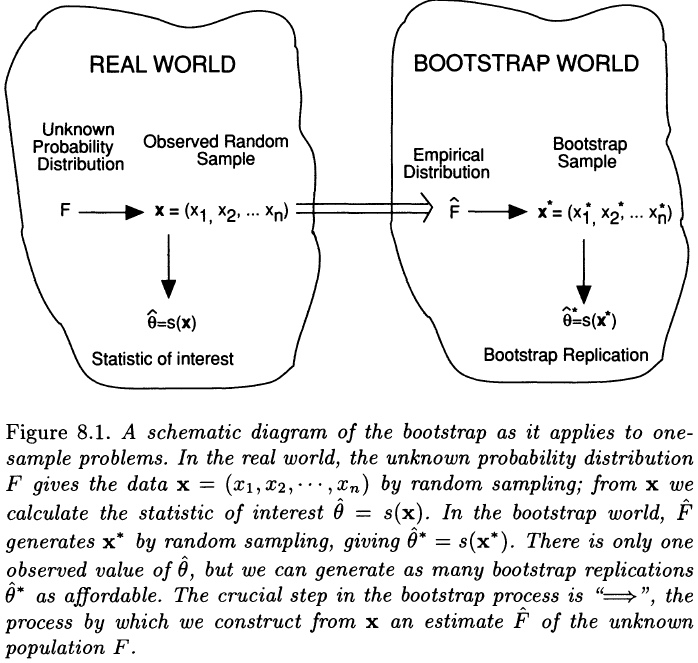
\includegraphics[width=\linewidth]{8/f81}
\newline

В правой части рисунка находится мир бутстрепа, если использовать терминологию Дэвида Фридмана. В мире бутстрепа эмпирическое распределение $\hat{F}$ порождает бутстреп выборки $\textbf{x}^* = (x_1^*, x_2^*, \ldots, x_n^*)$ путем генерации случайной выборки, на основе которой мы вычисляем бутстреп репликации интересующей статистики, $\hat{\theta}^* = s(\textbf{x}^*)$. Большим преимуществом мира бутстрепа является то, что мы можем вычислить столько репликаций $\hat{\theta}^*$, сколько захотим, или, по крайней мере, столько, сколько мы можем себе позволить. Это позволяет нам делать вероятностные вычисления напрямую, например, используя наблюдаемую изменчивость $\hat{\theta}^*$ для оценки ненаблюдаемой величины $\text{se}_F(\hat{\theta})$.

Двойная стрелка на рис. 8.1 указывает на вычисление $\hat{F}$ из $F$. По идее, это решающий шаг в процессе бутстрепа, даже несмотря на то, что он прост в вычислительном отношении. Любая другая часть картины бутстрепа определяется аналогично: $F$ порождает $\textbf{x}$ путем генерации случайной выборки, поэтому $\hat{F}$ порождает $\textbf{x}^*$ путем генерации случайной выборки; $\hat{\theta}$ получается из $\textbf{x}$ через функцию $s(\textbf{x})$, поэтому $\hat{\theta}^*$ получается из $\textbf{x}^*$ таким же образом. Расчеты бутстрепа для более сложных вероятностных механизмов оказываются простыми, если мы знаем, как реализовать процесс, обозначенный двойной стрелкой --- оценку всего вероятностного механизма на основе данных. К счастью, это легко сделать для всех распространенных структур данных.

Чтобы облегчить изучение более сложных структур данных, мы будем использовать обозначение
\begin{equation}
	P \to \textbf{x},
\end{equation}
чтобы указать, что неизвестная \textit{вероятностная модель} $P$ породила наблюдаемый набор данных $\textbf{x}$.
\section{Двухвыборочная задача}

Чтобы понять обозначения (8.2), рассмотрим данные о мышах в таблице 2.1. Вероятностную модель $P$ можно представить как пару распределений вероятностей $F$ и $G$, первое для экспериментальной группы и второе для контрольной группы
\begin{equation}
	P = (F, G).
\end{equation}

Пусть $\textbf{z} = (z_1, z_2, \ldots, z_m)$ обозначает экспериментальные наблюдения, а $\textbf{y} = (y_1, y_2, \ldots, y_n)$ обозначает контрольные наблюдения с $n = 7$ и $m = 9$. Тогда наблюдаемые данные включают $\textbf{z}$ и $\textbf{y}$
\begin{equation}
	\textbf{x} = (\textbf{z}, \textbf{y}).
\end{equation}
Можем представить себе $\textbf{x}$ как $16$-мерный вектор, если мы помним, что семь элементов из $F$, девять --- из $G$. Отображение $P \to \bf{x}$ описывается следующим образом:
\begin{equation}
	F \to \textbf{z} \text{ независимо от } G \to \textbf{y}.
\end{equation}
Другими словами, $\textbf{z}$ --- это случайная выборка размера $7$ из $F$, $\textbf{y}$ --- случайная выборка размера $9$ из $G$, причем $\textbf{z}$ и $\textbf{y}$ взаимно независимы друг от друга. Такая постановка называется \textit{двухвыборочной задачей}. 

В этом случае легко оценить вероятностный механизм $P$. Пусть $\hat{F}$ и $\hat{G}$~--- эмпирические распределения, основанные на $\textbf{z}$ и $\textbf{y}$ соответственно. Тогда естественная оценка $P = (F, G)$ такова:
\begin{equation}
	\hat{P} = (\hat{F}, \hat{G}).
\end{equation}

После получения $\hat{P}$ определение бутстреп выборки $\textbf{x}^*$ очевидно, стрелка в выражении
\begin{equation}
	\hat{P} \to \textbf{x}^*
\end{equation}
должна означать то же самое, что и стрелка в $P \to \textbf{x}$, (8.2). В двухвыборочной задаче (8.5) мы имеем $\textbf{x}^* = (\textbf{z}^*, \textbf{y}^*)$, где
\begin{equation}
	\hat{F} \to \textbf{z}^* \text{ независимо от } \hat{G} \to \textbf{y}^*.
\end{equation}
Размеры выборки для $\textbf{z}^*$ и $\textbf{y}^*$ такие же, как для $\textbf{z}$ и $\textbf{y}$ соответственно.

На рисунке 8.2 показана гистограмма $B = 1400$ бутстреп репликаций статистики $\hat \theta$
 \begin{align}
 	\hat{\theta} & = \hat{\mu}_z - \hat{\mu}_y = \bar{z} - \bar{y} = \notag \\
 	& = 86.86 - 56.22 = 30.63,
 \end{align}
где $\hat \theta$ --- разность в средних значениях экспериментальной и контрольной групп в данных о мышах. Эта статистика оценивает параметр
\begin{equation}
	\theta = \mu_z - \mu_y = \text{E}_f(z) - \text{E}_G(y).
\end{equation}
Если $\theta$ действительно намного больше $0$, как, по-видимому, указывает (8.9), то экспериментальная группа показывает гораздо лучший результат по сравнению с контрольной группой. Однако бутстреп оценка стандартной ошибки для $\hat{\theta} = 30.63$ это
\begin{equation}
	\widehat{\text{se}}_{1400} = \left\{ \sum_{b=1}^{1400} [ \hat{\theta}^*(b) - \hat{\theta}^*(\cdot) ]^2 / 1399 \right\}^{1/2} = 26.85,
\end{equation}
поэтому $\hat{\theta}$ всего лишь на $1.14$ стандартной ошибки больше нуля, $1.14 = 30.63 / 26.85$. Обычно такой результат не считается убедительным доказательством того, что истинное значение $\theta$ больше $0$.

Бутстреп репликации $\hat{\theta}^*$ были получены при помощи генератора случайных чисел для соблюдения независимости (8.8). Каждая бутстреп выборка $\textbf{x}^*$ вычислена следующим образом
\begin{equation}
	\textbf{x}^* = (\textbf{z}^*, \textbf{y}^*) = (z_{i_1}, z_{i_2}, \ldots, z_{i_7}, y_{j_1}, y_{j_2}, \ldots, y_{j_9}),
\end{equation}

\noindent где $(i_1, i_2, \ldots, i_7)$ есть случайная выборка размера $7$ из целых чисел $1,2,\ldots,7$, а $(j_1, j_2, \ldots, j_g)$ есть независимо выбранная случайная выборка размера $9$ из целых чисел $1, 2, \ldots, 9$. Например, первая бутстреп выборка $(i_1, i_2, \ldots, i_7) = (7,3,1,2,7,6,3)$ и $(j_1, j_2, \ldots, j_9) = (7,8,2,9,6,7,8,4,2)$.

Стандартная ошибка $\theta$ может быть записана как $\text{se}_P(\hat{\theta})$, чтобы подчеркнуть тот факт, что она зависит от неизвестного вероятностного механизма $P = (F, G)$. Бутстреп оценка $\text{se}_P(\hat{\theta})$ --- это оценка методом подстановки
\begin{equation}
	\text{se}_{\hat{P}}(\hat{\theta}^*) = \{ \text{var}_{\hat{P}}(\bar{z}^* - \bar{y}^*) \}^{1/2}.
\end{equation}
Как и в главе 6, мы аппроксимируем идеальную бутстреп оценку $\text{se}_{\hat{P}}(\hat{\theta}^*)$ при помощи $\widehat{\text{se}}_B$ из уравнения (6.6), в данном случае при $B = 1400$. Тот факт, что $\hat{\theta}^*$ вычисляется из двух выборок, $\textbf{z}^*$ и $\textbf{y}^*$ не влияет на определение (6.6), а именно $\widehat{\text{se}}_B = \left\{ \sum_{b=1}^{B} [\hat{\theta}^*(b) - \hat{\theta}^*(\cdot)]^2/(B-1) \right\}^{1/2}$.

\noindent
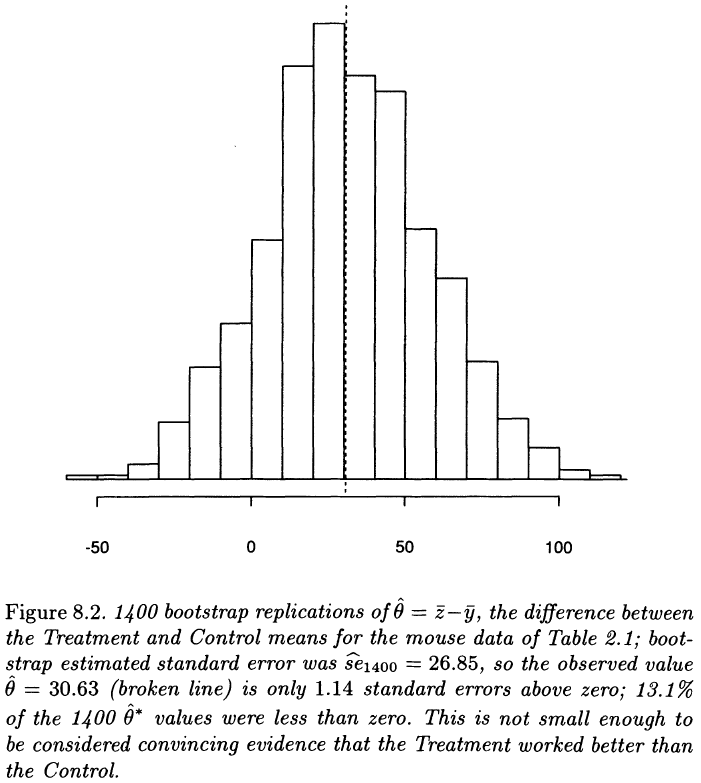
\includegraphics[width=\linewidth]{8/f82}
\newline
\section{Более общие структуры данных}

Рисунок 8.3 --- это версия рисунка 8.1, в применении к общим структурам данных $P \to \textbf{x}$. Между этими двумя рисунками нет особой концептуальной разницы, за исключением уровня обобщения. В реальном мире неизвестный вероятностный механизм $P$ порождает наблюдаемый набор данных $\textbf{x}$ в соответствии с правилом построения, указанным стрелкой «$\to$». В конкретных приложениях нам нужно более тщательно определять стрелку, наподобие того как в (8.5) для двухвыборочной задачи. Набор данных $\textbf{x}$ больше не может быть одним вектором. Он имеет форму, зависящую от структуры данных, например $\textbf{x} = (\textbf{z}, \textbf{y})$ в двухвыборочной задаче.\\
\noindent
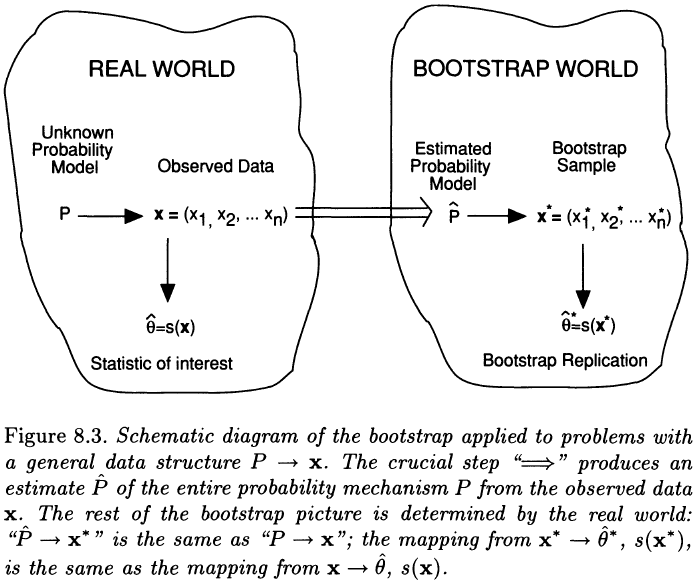
\includegraphics[width=\linewidth]{8/f83}
\newline
\noindent Наблюдая за $\textbf{x}$, мы вычисляем интересующую статистику $\hat{\theta}$ из $\textbf{x}$ в соответствии с функцией $s(\cdot)$.

Бутстреп часть на рис. 8.3 описывается аналогичными понятиями и в реальном мире: стрелка в $\hat{P} \to \textbf{x}^*$ означает то же самое, что и стрелка в $P \to \textbf{x}$. И функция, отображающая $\textbf{x}^*$ в $\hat{\theta}^*$, является той же функцией $s(\cdot)$, что и отображающая $\textbf{x}$ в $\hat{\theta}$. 

При фактическом проведении бутстреп анализа на основе рисунка 8.3 возникают две практические задачи:

(1). Нам нужно оценить весь вероятностный механизм $P$ по наблюдаемым данным $\textbf{x}$. Это шаг, обозначенный двойной стрелкой $\textbf{x} \Rightarrow \hat{P}$. Это удивительно легко сделать для большинства знакомых структур данных. Универсального рецепта нет, но в каждом отдельном случае доступны вполне обычные конкретные решения, например, $\hat{P} = (\hat{F}, \hat{G})$ для двухвыборочной задачи. Дополнительные примеры приведены в этой и следующей главах.

(2). Нам нужно смоделировать бутстреп данные из $\hat{P}$ в соответствии с подходящей структурой данных. Это шаг $\hat{P} \to \textbf{x}^*$ изображен на рисунке 8.3. Этот шаг концептуально прост, будучи таким же, как $P \to \textbf{x}$, но может потребовать некоторой осторожности при программировании, если необходима вычислительная эффективность. (Мы увидим пример данных про анализ лютенизирующего гормона ниже.) Обычно генерация бутстреп данных $\hat{P} \to \textbf{x}^*$ требует меньше времени, чем вычисление $\hat{\theta}^* = s(\textbf{x}^*)$.

\noindent
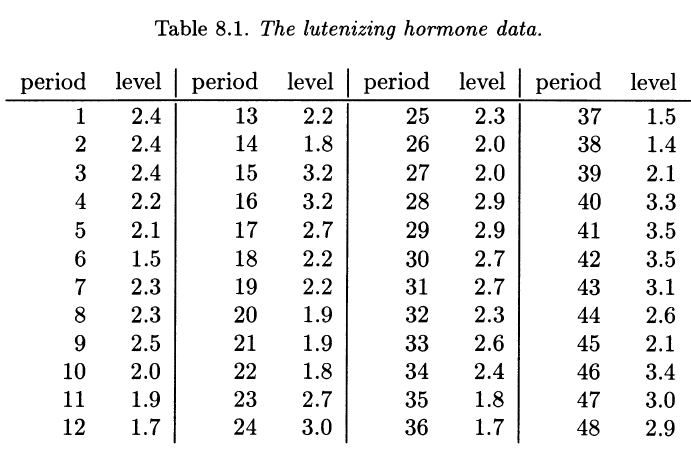
\includegraphics[width=12cm]{8/t81}\\
\section{Пример: лютеинизирующий гормон}

На рис. 8.4 показан набор данных про уровень $y_t$ лютенизирующего гормона для каждого из $48$ отрезков времени, взятых из Diggle (1990); набор данных приведен в таблице 8.1. Это данные об уровне гормона, измеренные у здоровой женщины с $10$-минутными интервалами в течение $8$ часов. Лютенизирующий гормон является одним из гормонов, регулирующих менструальный цикл, и поэтому важно понимать его суточные колебания. 

Понятно, что уровни гормона не являются случайной выборкой из какого-либо распределения. На рисунке 8.4 слишком много данных. Эти данные являются примером \textit{временного ряда}: структуры данных, для которой близкие значения временного параметра $t$ указывают тесно связанные значения измеренной величины $y_t$. Для анализа временных рядов используются многие интересные вероятностные модели. Мы начнем с простейшей модели~--- \textit{схемы авторегрессии первого порядка}.

Пусть $\mu$ --- математическое ожидание $y_t$, которое предполагается одинаковым для всех моментов времени $t$, и определим \textit{центрированные} измерения
\begin{equation}
	z_t = y_t - \mu.
\end{equation}
Все $z_t$ имеют математическое ожидание $0$. Схема авторегрессии первого порядка --- это одна из таких схем, в которой каждый $z_t$ является линейной комбинацией предыдущего значения $z_{t-1}$ и независимого шума $\varepsilon_t$,
\begin{equation}
	z_t = \beta z_{t-1} + \varepsilon_t \text{ для } t = U, U + 1, U + 2, \ldots, V.
\end{equation}

\noindent
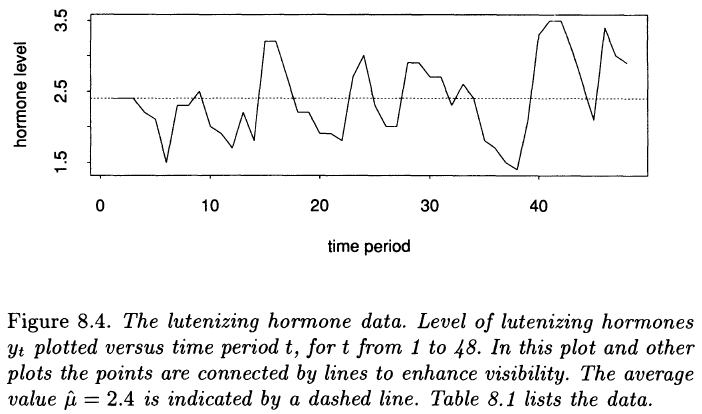
\includegraphics[width=12cm]{8/f84}
\newline
\noindent Здесь $\beta$ --- неизвестный параметр, действительное число от $-1$ до $1$. 

Предполагается, что шум $\varepsilon_t$ в (8.15) является случайной выборкой из неизвестного распределения $F$ с математическим ожиданием $0$,
\begin{equation}
	F \to (\varepsilon_U, \varepsilon_{U+1}, \varepsilon_{U+2}, \ldots, \varepsilon_V) \quad [\text{E}_F(\varepsilon) = 0].
\end{equation}
Точки $U$ и $V$ --- это начало и конец анализируемого периода времени. Здесь у нас есть
\begin{equation}
	U = 2 \quad \text{и} \quad V = 48.
\end{equation}
Обратите внимание, что первое уравнение в (8.15) имеет вид
\begin{equation}
	z_U = \beta z_{U-1} + \varepsilon_U,
\end{equation}
поэтому нам нужно число $z_{U-1}$, чтобы запустить процесс авторегрессии. В нашем случае $z_{U-1} = z_1$. 

Пусть мы считаем, что модель (8.15), (8.16), авторегрессионный процесс первого порядка, применима к данным лютенизирующего гормона. Как мы можем оценить значение $\beta$ по данным? Один из ответов основан на методе наименьших квадратов. Прежде всего, мы оцениваем математическое ожидание $\mu$ в (8.14) по наблюдаемому среднему значению $\bar{y}$ (это $2.4$ для данных лютенизирующего гормона) и задаем
\begin{equation}
	z_t = y_t - \bar{y}
\end{equation}
для всех значений $t$. В дальнейшем мы проигнорируем разницу между определениями (8.14) и (8.19). 

Предположим, что $b$ --- это любое предположение об истинном значении $\beta$ в (8.15). Определим остаточную квадратичную ошибку для этого предположения как
\begin{equation}
	\text{RSE}(b) = \sum_{t=U}^{V} (z_t - b_{z_{t-1}})^2.
\end{equation}
Используя (8.15) и тот факт, что $\text{E}_F(\varepsilon) = 0$, легко показать, что $\text{RSE}(b)$ имеет математическое ожидание 
\begin{equation*}
	\text{E}\left(\text{RSE}(b)\right) = (b-\beta)^2 \text{E} \left(\sum_{t=U}^{V} z_{t-1}^2 \right) + (V-U+1) \text{var}_F(\varepsilon).
\end{equation*}
 Оно минимизируется, когда $b$ равно истинному значению $\beta$. Мы убедились, что $\text{RSE}(b)$ должен достичь своего минимума где-то рядом с истинным значением $\beta$. 

Учитывая данные временного ряда, мы можем рассчитать $\text{RSE}(b)$ как функцию $b$, и выбрать минимизирующее значение, которое будет нашей оценкой $\beta$
\begin{equation}
	\text{RSE}(\hat{\beta}) = \min_b \text{RSE}(b).
\end{equation}
Данные про лютенизирующий гормон имеют следующую оценку наименьших квадратов
\begin{equation}
	\hat{\beta} = 0.586.
\end{equation}

Насколько точна оценка $\hat{\beta}$? Чтобы ответить на этот вопрос, мы можем использовать общую бутстреп процедуру, показанную на рис. 8.3. Вероятностный механизм $P$, описанный в (8.15), (8.16), имеет два неизвестных элемента, $\beta$ и $F$, скажем, $P = (\beta, F)$. (Здесь мы рассматриваем $\mu$ в (8.14) как известную и равную $\bar{y}$.) Данные $\textbf{x}$ состоят из наблюдений $y_t$ и соответствующих им периодов времени $t$. Мы знаем, что правило построения $P \to \textbf{x}$ описывается формулами (8.15)--(8.16). Интересующая статистика $\hat{\theta}$ равна $\hat{\beta}$, поэтому отображения $s(\cdot)$ неявно задаются (8.21).

Остается один шаг, прежде чем мы сможем применить бутстреп: шаг двойной стрелки $\textbf{x} \Rightarrow \hat{P}$, в котором $P = (\beta, F)$ оценивается по данным. Теперь $\beta$ уже была оценена с помощью $\hat{\beta}$, (8.21), поэтому нам нужно только оценить распределение отклонений $F$. Если бы мы знали $\beta$, то мы могли бы вычислить $\varepsilon_t = z_t - \beta z_{t-1}$ для каждого $t$ и оценить $F$ по эмпирическому распределению значений $\varepsilon_t$. Мы не знаем $\beta$, то мы можем использовать оценочное значение $\hat{\beta}$, чтобы вычислить \textit{отклонения [approximate disturbances]}
\begin{equation}
	\hat{\varepsilon}_t = z_t - \hat{\beta} z_{t-1} \text{ для } t = U, U + 1, U + 2, \ldots, V.
\end{equation}
Пусть $T = V - U + 1$, количество слагаемых в (8.23); $T = 47$ для выбора (8.17). Очевидная оценка $F$ --- это $\hat{F}$, эмпирическое распределение отклонений
\begin{equation}
	\hat{F}: \text{ вероятность } 1/T \text{ для } \hat{\varepsilon}_t \text{ при } t = U, U + 1, \ldots, V.
\end{equation}

На рис. 8.5 показана гистограмма отклонений $\hat{\varepsilon}_t = z_t - \hat{\beta} z_{t-1}$ с $T = 47$ для схемы авторегрессии первого порядка, примененной к данным о лютеинизирующем гормоне в промежутке от 2 до 48 лет.

\noindent
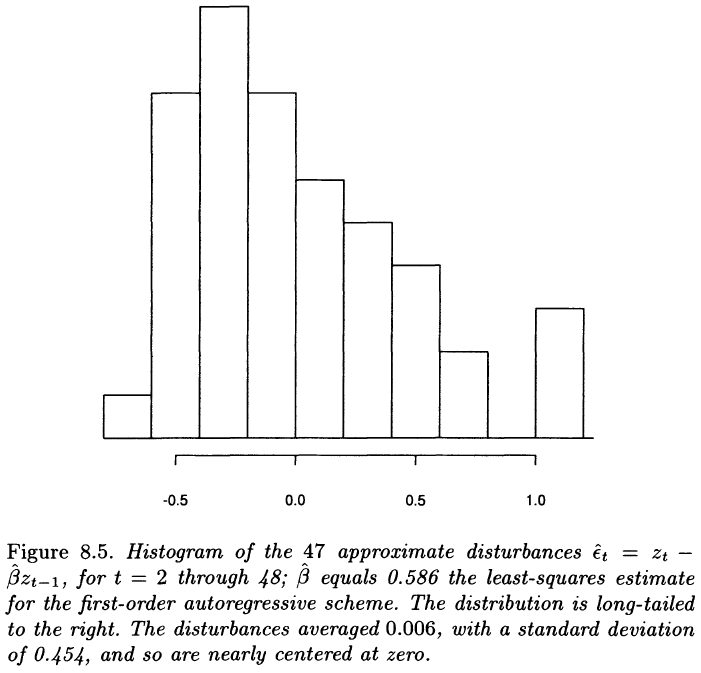
\includegraphics[width=\linewidth]{8/f85}
\newline

Мы видим, что распределение $\hat{F}$ не является нормальным и имеет длинный хвост справа. Распределение имеет среднее значение $0.006$ и стандартное отклонение $0.454$. Не случайно, что среднее значение $\hat{F}$ близко к $0$. Если бы это было не так, мы могли бы соблюдать определение $\text{E}_F(\varepsilon) = 0$ в (8.16) путём центрирования $\hat{F}$; то есть изменением каждой вероятностной точки в (8.23) от $\hat{\varepsilon}_t$ до $\hat{\varepsilon}_t - \bar{\varepsilon}$, где $\bar{\varepsilon} = \sum_{t=U}^{V} \hat{\varepsilon}_t/T$.

Теперь мы готовы провести бутстреп анализ точности оценки $\hat{\beta} = 0.586$. Набор бутстреп данных $\hat{P} \to \textbf{x}^*$ генерируется в соответствии с определениями (8.15)--(8.16), за исключением $\hat{P} = (\hat{\beta}, \hat{F})$, заменённого на $P = (\beta, F)$. Начнем с начального значение $z_1 = y_1 - \bar{y}$, которое считается фиксированной константой (как размер выборки $n$ в одновыборочной задаче). Бутстреп временной ряд $z_t^*$ вычисляется рекурсивно
\begin{align}
	z_2^* & = \hat{\beta} z_1 + \varepsilon_2^* \notag \\
	z_3^* & = \hat{\beta} z_2^* + \varepsilon_3^* \notag \\
	z_4^* & = \hat{\beta} z_3^* + \varepsilon_4^* \notag \\
	\vdots & \notag \\
	z_{48}^* & = \hat{\beta} z_{47}^* + \varepsilon_{48}^*.
\end{align}
Бутстреп остатки $\varepsilon_t^*$ представляют собой случайную выборку из $\hat{F}$,
\begin{equation}
	\hat{F} \to (\varepsilon_2^*, \varepsilon_2^*, \ldots, \varepsilon_{48}^*).
\end{equation}
Другими словами, каждый $\varepsilon_t^*$ равняется любому из $T$ отклонений (8.23) с вероятностью $1/T$.

Процесс бутстрепа (8.25)--(8.26) был запущен $B=200$ раз, что дало $200$ бутстреп временных рядов. Каждый из них дал бутстреп репликацию $\hat{\beta}^*$ для оценки $\hat{\beta}$ методом наименьших квадратов, (8.21). На рисунке 8.6 показана гистограмма из $200$ значений $\hat{\beta}^*$. Оценка бутстреп стандартной ошибки для $\hat{\beta}$ составляет $\hat{\text{se}}_{200} = 0.116$. Гистограмма имеет довольно нормальную форму.

В схеме авторегрессии первого порядка каждый $z_t$ зависит от своих предшественников только через значение $z_{t-1}$ (Этот вид зависимости известен как \textit{марковский процесс первого порядка}.) Схема авторегрессии второго порядка расширяет зависимость обратно до $z_{t-2}$,
\begin{align}
	z_t = \beta_1 z_{t-1} + \beta_2 z_{t-2} + \varepsilon_t \notag \\
	\text{для } t = U, U + 1, U + 2, \ldots, V.
\end{align}
Здесь $\bm \beta = (\beta_1, \beta_2)^\text{T}$ --- двумерный вектор неизвестных параметров. $\varepsilon_t$ --- независимые отклонения, как в (8.16). Согласно (8.18) исходные уравнения следующие 
\begin{align}
	z_U & = \beta_1 z_{U-1} + \beta_2 z_{U-2} + \varepsilon_U \notag \\
	z_{U+1} & = \beta_1 z_U + \beta_2 z_{U-1} + \varepsilon_{U+1},
\end{align}
поэтому нам нужны числа $z_{U-2}$ и $z_{U-1}$ для начала. Теперь $U = 3$, $V = 48$ и $T = V - U + 1 = 46$.

Метод наименьших квадратов непосредственно приводит к оценке вектора $\bm{\beta}$. Пусть $\textbf{z}$ является $T$-мерным вектором $(z_U, z_{U+1}, \ldots, z_V)^\text{T}$, и пусть $\textbf{Z}$~--- матрица $T \times 2$ с первым столбцом $(z_{U-1}, z_U, \ldots, z_{V-1})^\text{T}$, вторым столбцом $(z_{U-2}, z_{U-1}, z_U,  \ldots, z_{V-2})^\text{T}$. Тогда оценка $\bm{\beta}$ методом наименьших квадратов следующая
\begin{equation}
	\hat{\bm \beta} = (\textbf{Z}^\text{T} \textbf{Z})^{-1} \textbf{Z}^\text{T} \textbf{z}.
\end{equation}

\noindent
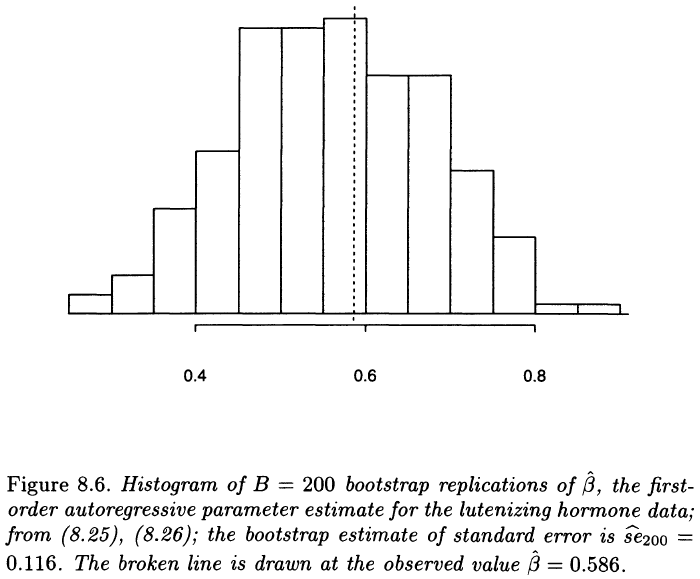
\includegraphics[width=\linewidth]{8/f86}
\newline

Для данных о лютенизирующем гормоне схема авторегрессии второго порядка имела следующие оценки наименьших квадратов
\begin{equation}
	\hat{\bm \beta} = (0.771, -0.222)^\text{T}.
\end{equation}
На рис. 8.7 показаны гистограммы с $B=200$ бутстреп репликациями из двух компонентов из $\hat{\bm \beta} = (\hat{\beta}_1, \hat{\beta}_2)^\text{T}$. Стандартные ошибки бутстрепа равны
\begin{equation}
	\widehat{\text{se}}_{200} (\hat \beta_1) = 0.147, \quad \widehat{\text{se}}_{200} (\hat \beta_2) = 0.149.
\end{equation}
Обе гистограммы приближенно имеют форму нормального распределения.

Схема авторегрессии второго порядка при $\beta_2 = 0$ является схемой авторегрессии первого порядка. При выполнении анализа точности для схемы второго порядка мы проверяем, не отклоняется ли $\hat \beta_2$ от $0$ менее чем на $2$ стандартные ошибки, что обычно интерпретируется как незначительное отличие $\hat \beta_2$ от $0$. Здесь $\hat \beta_2$ --- это примерное отклонение на $1.5$ стандартные ошибки от $0$, и в этом случае у нас нет убедительных доказательств того, что схема авторегрессии первого порядка не дает разумного представления данных о лютеинизирующем гормоне.

Знаем ли мы наверняка, что схема первого порядка дает хорошее представление о ряде лютенизирующих гормонов? Мы не можем дать окончательный ответ на этот вопрос, не рассматривая еще более общие модели,
\noindent
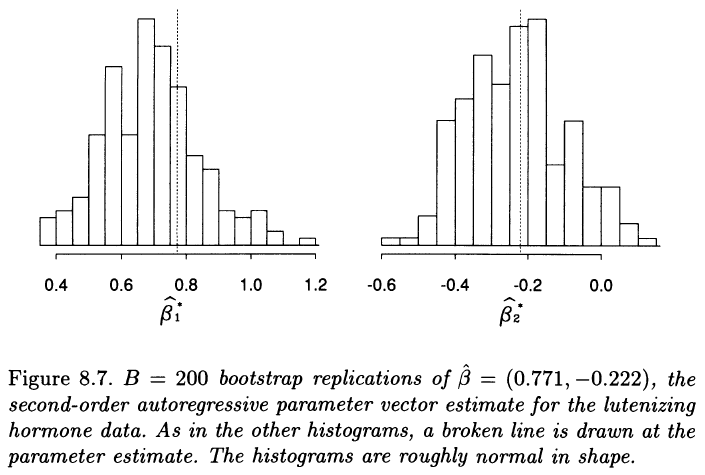
\includegraphics[width=\linewidth]{8/f87}
\newline
такие как схемы авторегрессии более высоких порядков. Приблизительный ответ может быть получен путем сравнения бустреп временных рядов с фактическими рядами на рис. 8.4. На рисунке 8.8 на левых графиках показаны первые четыре бустреп набора из первой схемы, правые четыре графика отображают реализации, полученные путем выборки с повторением из исходного временного ряда. Исходные данные на рис. 8.4 очень похожи на реализации левых графиков и совсем не похожи на реализации правых графиков.

Дальнейший анализ показывает, что модель AR(1) обеспечивает разумное соответствие этим данным. Однако нам потребуется более длительный временной ряд, чтобы эффективно различать разные модели для этого гормона.

В общем, стоит помнить, что математические модели представляют собой удобные упрощенные представления сложных явлений реального мира и иногда не совсем корректны. Часто необходим некоторый компромисс между усложнением модели и научными потребностями исследования. Методы бустрепа особенно полезны, если существует потребность в сложных моделях, поскольку математическая сложность не является препятствием для анализа точности бустрепа.\\
\section{Бутстреп скользящих окон}

\noindent
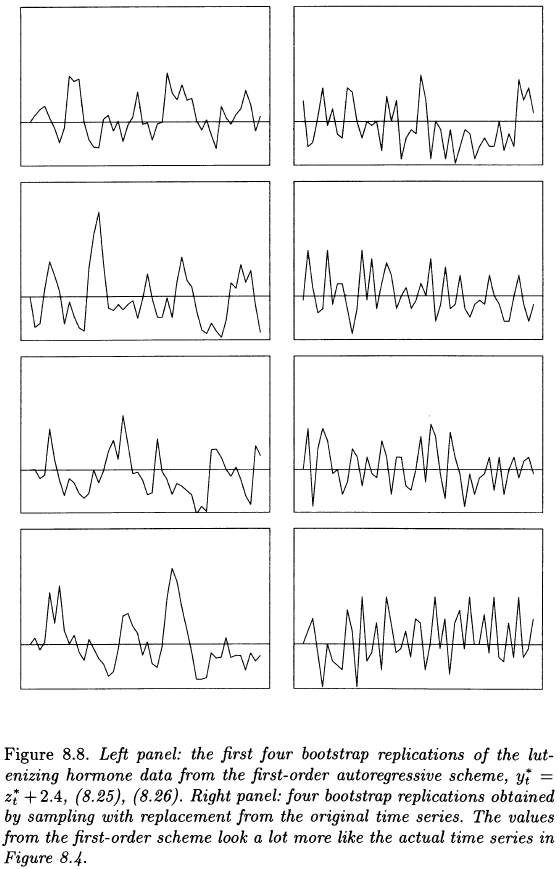
\includegraphics[width=\linewidth]{8/f88}
\newline

\noindent В этом разделе мы кратко опишем другой метод применения бутстрепа к временным рядам. Вместо подгонки модели и последующей выборки из остатков этот метод использует подход, более близкий к подходу, используемому для одновыборочных задач. Идея проиллюстрирована на рисунке 8.9. Исходный временной ряд представлен черными кружками. Чтобы сгенерировать бустреп реализацию временного ряда (белые кружки), мы выбираем длину окна («$3$» на диаграмме) и рассматриваем все возможные смежные окна этой длины. Мы составляем выборку с заменой из этих окон и объединяем их вместе, чтобы сформировать бутстреп временные ряды. Выбирается ровно столько окон, сколько необходимо для получения серии примерно такой же длины, что и исходная. Если длина окна равна $l$, то выберем $k$ окон так, чтобы $n \approx k \cdot l$.

Для иллюстрации мы выполним эти действия для данных о лютенизирующем гормоне. Интересующей статистикой была оценка $\hat \beta$ методом наименьших квадратов у AR(1). Мы выбрали длину окна $3$ и использовали бутстреп скользящих окон для генерации бустреп выборки для данных про лютенизирующий гормон. Типичная реализация бустрепа показана на рисунке 8.10, и она очень похожа на исходный временной ряд. Затем мы подогнали модель AR(1) к этому бутстреп временному ряду и оценили коэффициент $\hat \beta^*$ у AR(1). Весь этот процесс был повторен $B=200$ раз. (Обратите внимание, что модель AR(1) используется здесь для оценки $\beta$, но не используется при генерации бустреп реализаций временного ряда.) В результате стандартная ошибка бустрепа составила $\widehat {\text{se}}_{200} (\hat \beta) = 0.120$. Это примерно то же самое, что и значение $0.116$, полученное из AR(1) выборок, сгенерированных в предыдущем разделе. Увеличение размера окна до $5$ привело к уменьшению этого значения до $0.103$.

Чем оправдан бутстреп скользящих окон? Как мы видели ранее, мы не можем просто создать повторную выборку из отдельных наблюдений, так как это разрушило бы корреляцию, на которой мы хотим сфокусировать внимание. (Использование размера окна, равного единице, соответствует выборке с возвращением, и дает $0.139$ для оценки стандартной ошибки.) С бутстрепом скользящих окон идея состоит в том, чтобы выбрать размер окна $l$ достаточно большим, чтобы наблюдения, отстоящие более чем на $l$ единиц времени, были почти независимыми. Выбирая окна длиной $l$, мы сохраняем корреляцию, присутствующую в наблюдениях, отстоящих менее чем на $l$ единиц.

Бутстреп скользящих окон имеет то преимущество, что он менее «зависим от модели», чем подход бутстреп остатков, использовавшийся ранее. Как мы видели, последний метод зависит от модели, которая соответствует исходному временному ряду (например, модель AR(1) или AR(2)). Однако выбор размера окна $l$ может быть весьма важным, и эффективные методы для этого еще не разработаны.

В задаче регрессии, обсуждаемой в следующей главе, мы сталкиваемся с различными методами бустрепа, аналогичными подходам для временных рядов, которые мы обсуждали здесь.

\noindent
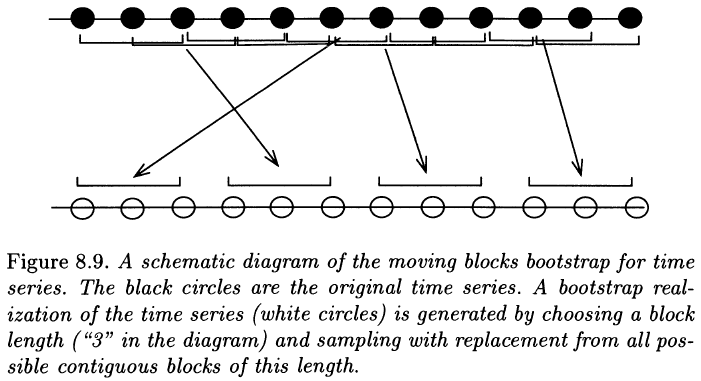
\includegraphics[width=\linewidth]{8/f89}
\newline

\noindent
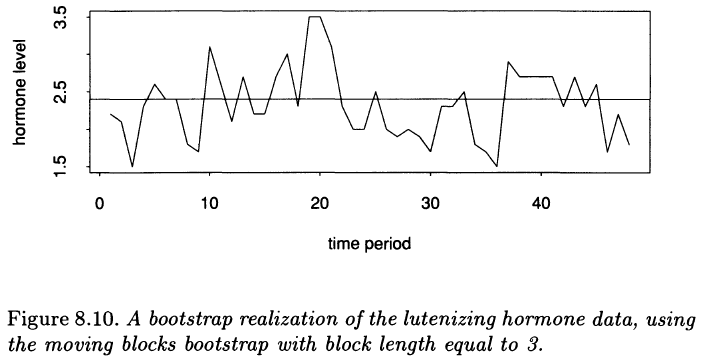
\includegraphics[width=\linewidth]{8/f810}
\newline
\section{Библиографические примечания}

Анализ временных рядов описан во многих книгах, включая Бокс and Дженкинс (1970), Чатфилд (1980) и Дигл (1990). Применение бутстрепа к временным рядам обсуждается в Эфрон and Тибширани (1986); Метод скользящих окон и связанные с ним техники можно найти у Карлштейн (1986), Киинч (1989), Луи и Сингх (1992) и Политис и Романо (1992).

\chapter{Модели регрессии}
\section{Введение}

Регрессионные модели являются одними из самых полезных и наиболее часто используемых статистических методов. Они предлагают относительно простой анализ сложных ситуаций, когда мы пытаемся отсортировать влияние многих возможных объясняющих переменных на зависимую переменную. В главе 7 мы используем алгоритм одновыборочного бутстрепа, алгоритм для анализа точности регрессионного анализа данных холостирамина из таблицы 7.4. Здесь мы более критически смотрим на задачу регрессии. Рассмотрен общий бутстреп алгоритм, показанный на рис. 8.3, что приводит к несколько иному бутстреп анализу для задач регрессии.
\section{Линейная регрессионная модель}

Мы начнем с классической модели линейной регрессии, или линейной модели, восходящей к Лежандру и Гауссу в начале 19 века. Набор данных $\textbf{x}$ для модели линейной регрессии состоит из $n$ точек $\textbf{x}_1, \textbf{x}_2, \ldots, \textbf{x}_n$, где каждый $\textbf{x}_i$ сам по себе является парой, скажем
\begin{equation}
	\textbf{x}_i = (\textbf{c}_i, y_i).
\end{equation}
Здесь $\textbf{c}_i$ --- это $1 \times p$ вектор $\textbf{c}_i = (c_{il}, c_{i2}, \ldots, c_{ip})$, называемый \textit{вектором признаков} или \textit{предиктором}, а $y_i$ --- действительное число, называемое \textit{ответом}.

Пусть $\mu_i$ указывает условное ожидание $i$-го ответа $y_i$ с учетом предиктора $\textbf{c}_i$,
\begin{equation}
	\mu_i = \text{E}(y_i|\textbf{c}_i) \quad (i = 1,2, \ldots, n).
\end{equation}
Ключевое предположение в линейной модели состоит в том, что $\mu_i$ представляет собой линейную комбинацию компонентов предиктора $\textbf{c}_i$,
\begin{equation}
	\mu_i = \textbf{c}_i \bm{\beta} = \sum\limits_{j=1}^{p} c_{ij} \beta_j.
\end{equation}
\textit{Вектор параметров}, или \textit{параметр регрессии}, $\bm{\beta} = (\beta_1, \beta_2, \ldots, \beta_p)^\text{T}$ неизвестен, обычная цель регрессионного анализа состоит в том, чтобы вывести $\bm{\beta}$ из наблюдаемых данных $\textbf{x} = (\textbf{x}_1, \textbf{x}_2, \ldots, \textbf{x}_n)$. В квадратичной регрессии (7.20) для данных холостирамина ответ $y_i$ --- это улучшение для $i$-го человека, признак $\textbf{c}_i$ --- это вектор $(1, z_i, z_i^2)$ и $\bm{\beta} = (\beta_0, \beta_1, \beta_2)^\text{T}$. \underline{Примечание}: «Линейность» в линейной регрессии относится к линейной форме математического ожидания (9.3). Нет никакого противоречия в том, что линейная модель (7.20) является квадратичной функцией $z$.

Вероятностная структура линейной модели обычно выражается как
\begin{equation}
	y_i = \textbf{c}_i \bm{\beta} + \varepsilon_i \quad \text{для} \quad i = 1,2,\ldots,n.
\end{equation}
Предполагается, что ошибка $\varepsilon_i$ в (9.4) является случайной выборкой из неизвестного \textit{распределения ошибок} $F$ с математическим ожиданием $0$,
\begin{equation}
	F \to (\varepsilon_1, \varepsilon_2, \ldots, \varepsilon_n) = \bm{\varepsilon} \quad [\text{E}_F(\bm{\varepsilon})=0].
\end{equation}

Заметим, что (9.4), (9.5) влекут
\begin{align}
	\text{E}(y_i|\textbf{c}_i) & = \text{E}(\textbf{c}_i \bm{\beta}+\varepsilon_i|\textbf{c}_i) = \text{E}(\textbf{c}_i \bm{\beta}|\textbf{c}_i) + \text{E}(\varepsilon_i|\textbf{c}_i) \notag \\
	& = \textbf{c}_i \bm{\beta},
\end{align}
что является предположением о линейности (9.3). Здесь мы использовали тот факт, что математическое ожидание $\text{E}(\varepsilon_i|\textbf{c}_i)$ совпадает с безусловным ожиданием $\text{E}(\varepsilon_i) = 0$, поскольку $\varepsilon_i$ выбираются независимо от $\textbf{c}_i$.

Мы хотим оценить вектор коэффициентов $\bm{\beta}$ из наблюдаемых данных $(\textbf{c}_1, y_1), (\textbf{c}_2, y_2), \ldots, (\textbf{c}_n, y_n)$. Пробное значение $\bm{\beta}$, скажем $\textbf{b}$, дает \textit{остаточную квадратичную ошибку}
\begin{equation}
	\text{RSE}(\textbf{b}) = \sum\limits_{i=1}^{n} (y_i - \textbf{c}_i \textbf{b})^2,
\end{equation}
как в уравнении (7.21). Оценка \textit{методом наименьших квадратов} $\bm{\beta}$ --- это значение $\hat{\bm{\beta}}$ из $\textbf{b}$, которое минимизирует $\text{RSE}(\textbf{b})$,
\begin{equation}
	\text{RSE}(\hat{\bm{\beta}}) = \min_{\textbf{b}} [\text{RSE(\textbf{b})}].
\end{equation}
Пусть $\textbf{C}$ --- матрица размерности $n \times p$ с $i$-й строкой $\textbf{c}_i$, а \textbf{y} --- вектор $(y_1, y_2, \ldots, y_n)^\text{T}$. Тогда оценка методом наименьших квадратов является решением следующего уравнения
\begin{equation}
	\textbf{C}^\text{T} \textbf{C} \hat{\bm{\beta}} = \textbf{C}^\text{T} \textbf{y}
\end{equation}

\noindent
\noindent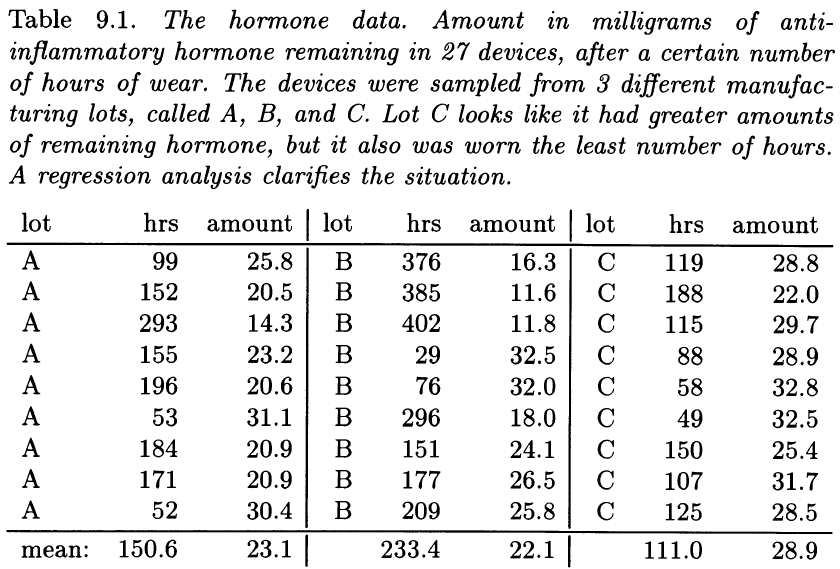
\includegraphics[width=\linewidth]{9/t91}
\newline
и задается формулой
\begin{equation}
	\hat{\bm{\beta}} = (\textbf{C}^\text{T} \textbf{C})^{-1} \textbf{C}^\text{T} \textbf{y}.
\end{equation}
\section{Пример: данные по гормонам}

В таблице 9.1 показан небольшой набор данных, который является подходящим для регрессионного анализа. Медицинское устройство для непрерывной доставки противовоспалительного гормона было протестировано на $27$ пациентах. Переменная ответа $y_i$ --- это количество гормона, оставшееся в устройстве после ношения,
$$y_i = \text{ оставшееся количество гормона в устройстве } i, \; i = 1, 2, \ldots, 27.$$
Есть две переменные--предикторы,
$$z_i = \text{ количество часов ношения i-го устройства}$$
и
$$L_i = \text{ производственная партия устройства i}.$$
Тестируемые устройства были случайным образом выбраны из трех различных производственных партий, названных $A$, $B$ и $C$.

Левая часть рисунка 9.1 представляет собой диаграмму рассеяния 27 точек $(z_i, y_i) = (\text{часы}_i, \text{число}_i)$ с символом $L_i$, используемым в качестве графического сивола. Мы видим, что более длительное время ношения приводит к меньшему количеству оставшегося гормона, как и следовало ожидать. Мы можем количественно оценить это наблюдение с помощью регрессионного анализа.

Рассмотрим модель, в которой математическое ожидание $y$ является линейной функцией $z$,
\begin{equation}
	\mu_i = \text{E}(y_i|z_i) = \beta_0 + \beta_1 z_i \quad i = 1,2, \ldots, 27.
\end{equation}
Эта модель игнорирует $L_i$: она имеет форму (9.3) с векторами признаков размерности $p = 2$,
\begin{equation}
	\textbf{c}_i = (1, z_i).
\end{equation}
Вектор неизвестных параметров $\bm{\beta}$ был помечен $(\beta_0, \beta_1)$ вместо $(\beta_1, \beta_2)$, так что индексы соответствуют степеням $z$, как в (7.20). Нормальные уравнения (9.10) дают оценку по методу наименьших квадратов
\begin{equation}
	\hat{\bm{\beta}} = (34.17, -0.0574)^\text{T}.
\end{equation}
Линия регрессии, оцененная методом наименьших квадратов
\begin{equation}
	\hat{\mu}_i = \textbf{c}_i \hat{\bm{\beta}} = \hat{\beta}_0 + \hat{\beta}_1 z_i
\end{equation}
изображена на правой части рисунка 9.1. Среди всех возможных линий, которые можно было нарисовать, эта линия минимизирует сумму квадратов $27$ вертикальных расстояний от точек до линии.

Насколько точен оценочный вектор параметров $\hat{\bm{\beta}}$? Ответ дает чрезвычайно полезная формула, также восходящая к Лежандру и Гауссу. Пусть $\textbf{G}$ --- матрица скалярных произведений $p \times p$,
\begin{equation}
	\textbf{G} = \textbf{C}^\text{T}\textbf{C},
\end{equation}
матрица с элементом $g_{hj} = \sum\limits_{i=1}^{n} c_{ih} c_{ij}$ в строке $h$, столбце $j$. Пусть $\sigma^2_F$ будет дисперсией ошибок в модели (9.4),
\begin{equation}
	\sigma^2_F = \text{var}_F(\varepsilon).
\end{equation}

Тогда стандартная ошибка $j$-го компонента $\hat{\bm{\beta}}$, квадратного корня из его дисперсии, равна
\begin{equation}
	\text{se}(\hat{\beta}_j) = \sigma_F \sqrt{G^{jj}}
\end{equation}
где $G^{jj}$ --- $j$-й диагональный элемент обратной матрицы $\textbf{G}^{-1}$.

\noindent
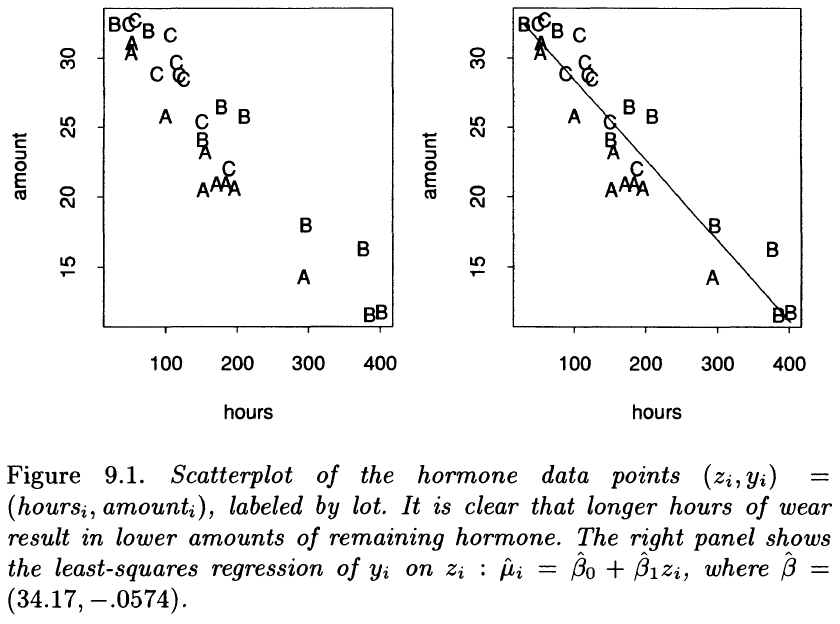
\includegraphics[width=\linewidth]{9/f91}
\newline

Последняя формула является обобщением формулы (5.4) для стандартной ошибки выборочного среднего, $\text{se}_F(\bar{x}) = \sigma_F / \sqrt{n}$, см. задачу 9.1. На практике $\sigma_F$ оценивается по формуле, аналогичной (5.11),
\begin{equation}
	\hat{\sigma}_F = \left\{ \sum\limits_{i=1}^{n} (y_i - \textbf{c}_i \hat{\bm{\beta}})^2 / n \right\}^{1/2} = \{ \text{RSE}(\hat{\bm{\beta}})/n \}^{1/2}
\end{equation}
или версией $\hat{\sigma}_F$ с корректированным смещением,
\begin{equation}
	\bar{\sigma}_F = \{ \text{RSE}(\hat{\bm{\beta}})/(n-p) \}^{1/2}.
\end{equation}
Соответствующие оценочные стандартные ошибки для компонентов $\hat{\bm{\beta}}$ равны
\begin{equation}
	\widehat{\text{se}}(\hat{\beta}_j) = \hat{\sigma}_F \sqrt{G^{jj}} \quad \text{или} \quad \overline{\text{se}} (\hat{\beta}_j) = \hat{\sigma}_F \sqrt{G^{jj}}.
\end{equation}
Связь между $\widehat{\text{se}}(\hat{\beta}_j)$ и $\overline{\text{se}}(\hat{\beta}_j)$ такая же, как между формулами (5.12) и (2.2) для среднего.

\noindent
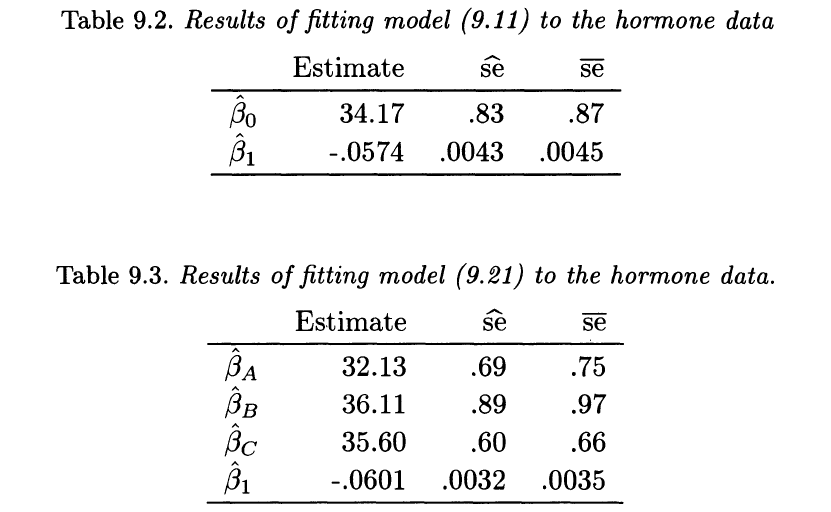
\includegraphics[width=\linewidth]{9/t92t93}
\newline

Большинство программ для линейной регрессии с библиотеками обычно выдают результат $\bar{\text{se}}(\hat{\beta}_j)$ вместе с оценкой $\hat{\beta}_j$ методом наименьших квадратов. Применение такой программы к модели (9.11) для данных по гормону дает результаты в таблице 9.2.

Глядя на правую часть рисунка 9.1, большинство точек для партии $A$ лежат ниже подобранной линии регрессии, в то время как большинство точек для партий $B$ и $C$ лежат выше этой линии. Это говорит о неточности модели (9.11). Если бы модель была точной, можно было бы ожидать, что примерно половина каждой партии будет лежать выше, а половина ниже установленной линии. Выражаясь обычной терминологией, похоже, что в данных присутствует эффект партии.

В нашу линейную модель легко включить эффект партии. Мы предполагаем, что условное математическое ожидание $y$ при заданных $L$ и $z$ имеет вид
\begin{equation}
	\text{E}(y|L,z) = \beta_L + \beta_1 z.
\end{equation}
Здесь $B_L$ равно одному из трех возможных значений: $\beta_A, \beta_B, \beta_C$, в зависимости от партии устройства. Это похоже на модель (9.11), за исключением того, что (9.21) допускает разные точки пересечения для каждой партии, а не одну точку пересечения $\beta_0$ из (9.11). Анализ модели (9.21) методом наименьших квадратов дал результаты в таблице 9.3.

Обратите внимание, что $\hat{\beta}_A$ на несколько стандартных ошибок меньше чем $\hat{\beta}_B$ и $\hat{\beta}_C$, что указывает на то, что устройства в партии $A$ содержат значительно меньше гормона.
\section{Применение бутстрепа}

Пока ни один из расчетов не требует бутстрепа. Однако полезно выполнить бутстреп-анализ для модели линейной регрессии. Оказывается, оценки стандартной ошибки бустрепа такие же, как $\widehat{\text{se}}(\hat{\beta}_j)$, (9.20). Убедившись, что бутстреп дает разумные ответы в случае, который мы можем проанализировать математически, мы можем продолжить применять бутстреп к более общим моделям регрессии, которые не имеют математического решения: где функция регрессии нелинейна по параметрам $\bm{\beta}$, и где мы используем методы подбора, отличные от метода наименьших квадратов.

Вероятностная модель $P \to \textbf{x}$ для линейной регрессии, как описано в (9.4), (9.5), состоит из двух компонентов:
\begin{equation}
	P = (\bm{\beta}, F),
\end{equation}
где $\bm{\beta}$ --- вектор параметров коэффициентов регрессии, а $F$ --- распределение вероятностей ошибок. Общий алгоритм бустрепа на рис. 8.3 требует, чтобы мы оценили $P$. У нас уже есть доступная $\hat{\bm{\beta}}$ --- оценка методом наименьших квадратов для $\bm{\beta}$. Как мы можем оценить $F$? Если предположить, что $\bm{\beta}$ известно, мы могли бы вычислить ошибки $\varepsilon_i = y_i - \textbf{c}_i \bm{\beta}$ для $i = 1,2, \ldots, n$ и оценить $F$ по их эмпирическому распределению. Мы не знаем $\bm{\beta}$, но можем использовать $\hat{\bm{\beta}}$ для вычисления аппроксимаций ошибок
\begin{equation}
	\hat{\varepsilon}_i = y_i - \textbf{c}_i \hat{\bm{\beta}}, \text{  для  } i = 1,2, \ldots, n.
\end{equation}
($\hat{\varepsilon}_i$ также называют \textit{остатками}.) Очевидная оценка $F$ --- это эмпирическое распределение $\hat{\varepsilon}_i$,
\begin{equation}
	\hat{F}: \text{ вероятность } 1/n \text{ для } \hat{\varepsilon}_i \text{ при } i = 1,2, \ldots, n.
\end{equation}
Обычно $\hat{F}$ будет иметь математическое ожидание $0$, как требуется в (9.5).

Имея $\hat{P} = (\hat{\bm{\beta}}, \hat{F})$, мы знаем, как рассчитать бутстреп наборы данных для модели линейной регрессии, в этом случае вероятностный механизм $\hat{P} \to \textbf{x}^*$ должен означать то же самое, что и вероятностный механизм $P \to \textbf{x}$, дающий фактический набор данных $\textbf{x}$, см. (9.4), (9.5). Чтобы сгенерировать $\textbf{x}^*$, мы сначала выбираем случайную выборку бустреп ошибок
\begin{equation}
	\hat{F} \to (\varepsilon_1^*, \varepsilon_2^*, \ldots, \varepsilon_n^*) = \bm{\varepsilon}^*.
\end{equation}
Каждый $\varepsilon_i^*$ равен любому из $n$ значений $\hat{\varepsilon}_j$ с вероятностью $1 / n$. Затем бустреп ответы $y_i^*$ генерируются согласно (9.4),
\begin{equation}
	y_i^* = \textbf{c}_i \hat{\bm{\beta}} + \varepsilon_i^* \text{  для  } i = 1,2,\ldots,n.
\end{equation}
Читатель должен убедиться, что формулы (9.24), (9.25), (9.26) есть то же самое, что (9.4), (9.5), за исключением того, что $\hat{P} = (\hat{\bm{\beta}}, \hat{F})$ заменяет $P = (\bm{\beta}, F)$. Обратите внимание, что $\hat{\bm{\beta}}$ --- фиксированная величина в (9.26), имеющая одинаковые значения для всех $i$.

Бутстреп набор данных $\textbf{x}^*$ представляет из себя $(\textbf{x}_1^*, \textbf{x}_2^*, \ldots, \textbf{x}_n^*)$, где $\textbf{x}_i^* = (\textbf{c}_i, y_i^*)$. Может показаться странным, что векторы признаков $\textbf{c}_i$ для бутстреп данных такие же, как и для фактических данных. Это происходит потому, что мы рассматриваем $\textbf{c}_i$ как фиксированные величины, а не как случайные. (Во всех наших примерах размер выборки $n$ трактовался одинаково.) Этот момент дополнительно обсуждается ниже.

Бустреп оценка $\hat{\bm{\beta}}^*$ методом наименьших квадратов является минимизатором квадратичной остаточной ошибки для бустреп данных,
\begin{equation}
	\sum\limits_{i=1}^{n}(y_i^* - \textbf{c}_i \hat{\bm{\beta}}^*)^2 = \min_{\textbf{b}} (y_i^* - \textbf{c}_i \textbf{b})^2.
\end{equation}
Нормальные уравнения (9.10), примененные к бутстреп данным, дают
\begin{equation}
	\hat{\bm{\beta}}^* = (\textbf{C}^\text{T} \textbf{C})^{-1} \textbf{C}^\text{T} \textbf{y}^*.
\end{equation}

В этом случае нам не нужны симуляции Монте--Карло, чтобы вычислить бутстреп стандартные ошибки для компонентов $\hat{\bm{\beta}}^*$. Несложный расчет дает выражение в явной форме для $\text{se}_{\hat{F}} (\hat{\bm{\beta}}_j^*) = \widehat{\text{se}}_{\infty} (\hat{\beta}_j)$, идеальной оценки бутстреп стандартной ошибки:
\begin{align}
	\text{var}(\hat{\bm{\beta}}^*) & = (\textbf{C}^\text{T} \textbf{C})^{-1} \textbf{C}^\text{T} \text{var}(\textbf{y}^*) \textbf{C}(\textbf{C}^\text{T} \textbf{C})^{-1} = \notag \\
	& = \hat{\sigma}_F^2 (\textbf{C}^\text{T} \textbf{C})^{-1},
\end{align}
поскольку $\text{var}(\textbf{y}^*) = \hat{\sigma}^2_F \textbf{I}$, где $\textbf{I}$ --- единичная матрица. Следовательно
\begin{equation}
	\widehat{\text{se}}_{\infty}(\hat{\beta}_j) = \hat{\sigma}_F \sqrt{G^{jj}}.
\end{equation}
Другими словами, бутстреп оценка стандартной ошибки для $\hat{\beta}_j$ такая же, как и обычная оценка $\widehat{\text{se}}(\hat{\beta}_j)$, (9.20).
\section{Бутстреп-пары против бутстреп-остатков}

Читатель, возможно, заметил интересный факт, теперь у нас есть два различных способа построения бутстреп регрессионной модели. Метод, описанный в главе 7, выбирает пары $\textbf{x}_i = (\textbf{c}_i, y_i)$, так что бутстреп набор данных $\textbf{x}^*$ имел форму
\begin{equation}
	\textbf{x}^* = \{ (\textbf{c}_{{i}_1}, y_{{i}_1}), (\textbf{c}_{{i}_2}, y_{{i}_2}), \ldots, (\textbf{c}_{{i}_n}, y_{{i}_n}) \},
\end{equation}
для $i_1, i_2, \ldots, i_n$ в случайной выборке целых чисел от $1$ до $n$. Обсуждаемый в этой главе метод (9.24), (9.25), (9.26) можно назвать «бутстрепом остатков». Он создает бутстреп наборы данных в форме
\begin{equation}
	\textbf{x}^* = \{ (\textbf{c}_1, \textbf{c}_1 \hat{\bm{\beta}} + \hat{\varepsilon}_{{i}_1}), (\textbf{c}_2, \textbf{c}_2 \hat{\bm{\beta}} + \hat{\varepsilon}_{{i}_2}), \ldots, (\textbf{c}_n, \textbf{c}_n \hat{\bm{\beta}} + \hat{\varepsilon}_{{i}_n}) \}.
\end{equation}

\noindent
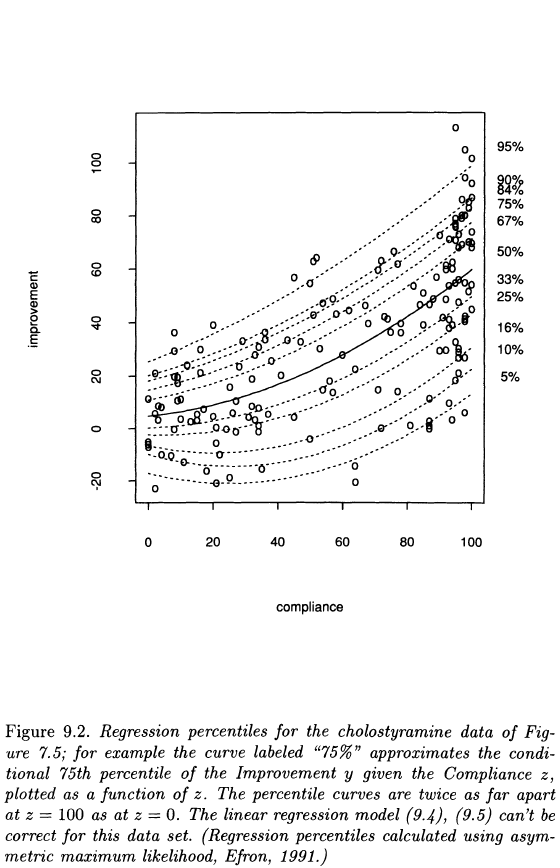
\includegraphics[width=\linewidth]{9/f92}
\newline

Какой бутстреп метод лучше? Ответ зависит от того, насколько мы доверяем модели линейной регрессии (9.4). Эта модель говорит, что разность между $y_i$ и его средним значением $\mu_i = \textbf{c}_i \bm{\beta}$ не зависит от $\textbf{c}_i$; он имеет одинаковое распределение «$F$» независимо от $\textbf{c}_i$. Это --- сильное предположение, которое может оказаться неверным, даже если модель математического ожидания $\mu_i = \textbf{c}_i \bm{\beta}$ верна. Это не соответствует данным про холостирамин на рис. 7.4.

На рисунке 9.2 показаны \textit{процентили регрессии} для данных про холостирамин. Например, кривая, обозначенная «$75$\%», аппроксимирует условный $75$-й процентиль показателя улучшения $y$ как функцию показателя соответствия $z$. Вблизи любого заданного значения $z$ около $75$\% нанесенных на график точек лежат ниже кривой. Модель (9.4), (9.5) предсказывает, что эти кривые будут находиться на одинаковом расстоянии друг от друга для всех значений $z$. Вместо этого кривые расходятся по мере увеличения $z$, находясь вдвое дальше друг от друга при $z = 100$, чем при $z = 0$. Другими словами, ошибки $\varepsilon_i$ в (9.4) стремятся быть вдвое больше при $z = 100$, чем при $z = 0$.

Бутстреп-пары менее чувствительны к предположениям, чем бутстреп-остатки. Стандартная оценка ошибки, полученная с помощью бутстреп-пар (9.31), дает разумные результаты, даже если (9.4), (9.5) полностью неверны. Единственное предположение, стоящее за (9.31), состоит в том, что исходные пары $\textbf{x}_i = (\textbf{c}_i, y_i)$ были случайным образом выбраны из некоторого распределения $F$, где $F$ --- распределение на $(p+1)$-мерных векторах $(\textbf{c}, y)$. Даже если (9.4), (9.5) верны, нет ничего плохого в бустреп-парах, как показано в (9.31); можно показать, что ответ (9.31) приближается к ответу (9.32) по мере увеличения числа пар $n$. Простая модель для данных о гормонах (9.12) была повторно проанализирована методом бутстреп-пар. $B = 800$ бутстреп-репликаций дали
\begin{equation}
	\hat{\text{se}}_{800} (\hat{\beta}_0) = 0.77 \quad \hat{\text{se}}_{800}(\hat{\beta}_1) = 0.0045,
\end{equation}
что не сильно отличается от результатов в таблице 9.2.

Можно привести и обратный аргумент. Модель (9.4), (9.5) не обязательно должна выполняться идеально, чтобы бутстреп остатков, как в (9.32), давал разумные результаты. Более того, различия в распределении ошибок, как и в данных о холостирамине, могут быть включены в модель (9.4), (9.5), что приведет к более подходящей версии бутстреп-остатков; см. модель (9.42). Возможно, наиболее важным моментом здесь является то, что бутстреп не является однозначно определенной концепцией. Рисунок 8.3 может быть реализован по-разному для одной и той же задачи, в зависимости от того, как интерпретируется вероятностная модель $P \to \textbf{x}$.

Когда мы осуществляем бустреп остатков, бутстреп наборы данных $\textbf{x}^* = \{(\textbf{c}_1, y_1^*), (\textbf{c}_2, y_2^*), \ldots, (\textbf{c}_n, y_n^*)\}$ имеют векторы признаков $\textbf{c}_1, \textbf{c}_2, \ldots, \textbf{c}_n$ в точности такие же, как и для фактического набора данных $\textbf{x}$. Это кажется неестественным для данных о гормонах, где $\textbf{c}_i$ включает $z_i$, затраченное количество часов, которое является такой же случайной величиной, как и переменная ответа $y_i$, оставшееся количество гормона.

Даже когда признаки генерируются случайным образом, есть причины проводить анализ так, как если бы они были фиксированными. Коэффициенты регрессии имеют большую стандартную ошибку, когда признаки имеют меньшее стандартное отклонение. Рассматривая признаки как фиксированные константы, мы получаем стандартную ошибку, которая отражает точность, связанную с выборкой фактически наблюдаемых признаков. Однако, как показывает (9.33), разница между $\textbf{c}_i$ фиксированной и $\textbf{c}_i$ случайной обычно не сильно влияет на оценку стандартной ошибки.
\section{Пример: данные о выживаемости клеток}

Бывают случаи в регрессии, когда признаки более естественно считать фиксированными, а не случайными. Данные по выживаемости клеток в таблице 9.4 показывают такую ситуацию. Радиолог провел эксперимент с 14 бактериальными пластинами. Пластинки подвергали воздействию различных доз радиации и измеряли долю выживших клеток. Как и следовало ожидать, более высокие дозы приводят к меньшей выживаемости. Знак вопроса после ответа на пластине $13$ отражает некоторую неуверенность в этом результате, выраженную исследователем.

Исследователя интересовал регрессионный анализ с переменной предиктором
\begin{equation}
	\text{доза}_i = z_i \quad i = 1,2, \ldots,14
\end{equation}
и переменной ответом
\begin{equation}
	\log \text{(пропорция выживания)}_i = y_i \quad i=1,2,\ldots,14.
\end{equation}
Были доступны две различные теоретические модели радиационного поражения, одна из которых предсказывала линейную регрессию
\begin{equation}
	\mu_i = \text{E}(y_i|z_i) = \beta_1 z_i,
\end{equation}
а другая квадратичную регрессию
\begin{equation}
	\mu_i = \text{E}(y_i|z_i) = \beta_1 z_i + \beta_2 z_i^2.
\end{equation}
В (9.36) или (9.37) нет пересекающих членов $\beta_0$, потому что мы знаем, что нулевая доза дает коэффициент выживаемости $1$, $y = \log (1) = 0$.

В таблице 9.5 показаны оценки по методу наименьших квадратов $(\hat{\beta}_1, \hat{\beta}_2)$ и их оценочные стандартные ошибки $\overline{\text{se}}(\hat{\beta}_j)$, (9.20). Представлены два анализа методом наименьших квадратов, один с данными для всех $14$ пластин, другой за исключением сомнительной пластины $13$. В обоих анализах оцененный коэффициент квадратичной регрессии $\hat{\beta}_2$ является положительным. Является ли это отличие значимым? Другими словами, можем ли мы заключить, что $\hat{\beta}_2$ останется положительным, если будет исследовано гораздо больше пластин? Отношение $\hat{\beta}_2/\widehat{\text{se}}(\hat{\beta}_2)$ помогает ответить на этот вопрос. 
\noindent
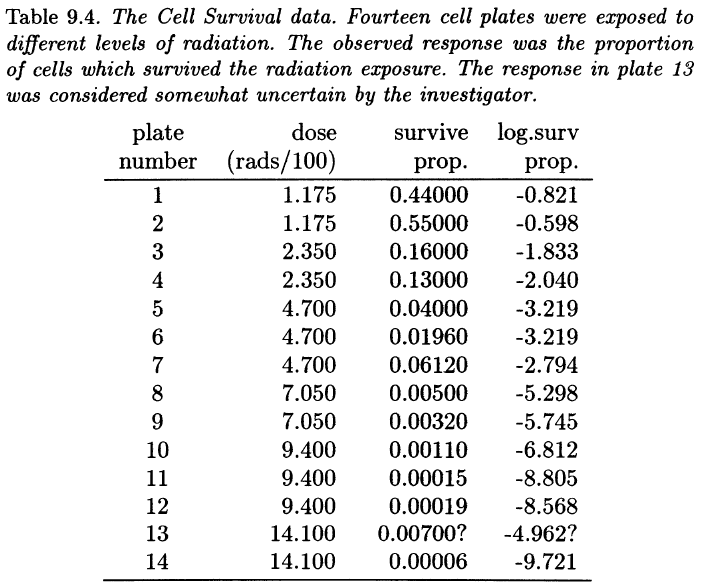
\includegraphics[width=\linewidth]{9/t94}
\newline
Отношение составляет $2.46$ для анализа, основанного на всех $14$ пластинах, что обычно считается убедительным доказательством того, что $\hat{\beta}_2$ значительно больше нуля. Если верить этому результату, то квадратичная модель (9.37) сильно предпочтительнее модели (9.36), которая имеет $\beta_2 = 0$.

Однако удаление сомнительной пластины $13$ из анализа снижает $\hat{\beta}_2/\widehat{\text{se}}(\hat{\beta}_j)$ только до $0.95$, что является незначимым результатом. Вывод заключается не в том, что $\beta_2$ \textit{обязательно} равен нулю, а в том, что он легко может быть равен нулю: если $\beta_2 = 0$, и если $(\beta_2) \dot = 0.0091$, как в строке 2 таблицы 9.5, то это вовсе не удивительно, что значение $\hat{\beta}_2$ такое же большое или больше наблюдаемого значения $0.0086$. Таким образом, у нас нет убедительных доказательств для отказа от линейной модели в пользу квадратичной модели.

Статистика --- это наука о сборе информации по крупицам с целью получения высокоинформативных сложных результатов. Статистики настораживаются, когда видят, что один элемент выборки, особенно подозрительный, доминирует в ответе на важный вопрос. Действительная критика регрессии по методу наименьших квадратов состоит в том, что один удаленный элемент, такой как пластина $13$, может иметь слишком большое влияние на подобранную кривую регрессии. Это показано на рисунке 9.3, на котором построена кривая регрессии методом наименьших квадратов как с пластиной $13$, так и без нее. Мощный эффект точки «?» очевиден.
\noindent
\includegraphics[width=\linewidth]{9/t95f93}
\newpage
\noindent Даже если бы исследователь не подвергал сомнению достоверность пластинки $13$, мы бы предпочли, чтобы наши подогнанные кривые не зависели так сильно от отдельных элементов выборки.
\section{Наименьшая медиана квадратов}

Наименьшая медиана квадратов регрессии, сокращенно $\text{LMS}$, является менее чувствительным методом подбора, чем метод наименьших квадратов. Единственное различие между методом наименьших квадратов и $\text{LMS}$ --- это выбор критерия соответствия. Чтобы обосновать критерий, давайте разделим остаточную квадратичную ошибку (9.7) на размер выборки, получив среднеквадратичные остатки
\begin{equation}
	\dfrac{1}{n} \sum\limits_{i=1}^{n} (y_i-\textbf{c}_i \textbf{b})^2.
\end{equation}
Минимизация (9.38), очевидно, то же самое, что минимизация (9.7). Средние выборок чувствительны к влияющим значениям, а медианы --- нет. Следовательно, чтобы сделать (9.38) менее чувствительным, мы можем заменить среднее значение на медиану, получив \textit{медиану квадратичных остатков}
\begin{equation}
	\text{MSR}(\textbf{b}) = \text{med}(y_i - \textbf{c}_i \textbf{b})^2.
\end{equation}
Оценка $\text{LMS}$ $\bm{\beta}$ --- это значение $\hat{\bm{\beta}}$, минимизирующее $\text{MSR(\textbf{b})}$,
\begin{equation}
	\text{MSR}(\hat{\bm{\beta}}) = \min_{\textbf{b}} [\text{MSR}(\textbf{b})].
\end{equation}

Обратите внимание, что разница между методом наименьших квадратов и $\text{LMS}$ заключается не в выборе модели, которая остается (9.3), а в том, как мы измеряем расхождения между моделью и наблюдаемыми данными. $\text{MSR}(\textbf{b})$ менее чувствителен, чем $\text{RSE}(\textbf{b})$, к удаленным точкам данных. Это можно увидеть на рис. 9.3, где, по-видимому, очень мало различий между квадратичной $\text{LMS}$-аппроксимацией с точкой «?» или без нее. На самом деле разницы нет. Расчетные коэффициенты регрессии равны $(\hat{\beta}_1, \hat{\beta}_2) = (-0.81, 0.0088)$ в обоих случаях.

Можно показать, что \textit{порог} (breakdown) оценки $\text{LMS}$ составляет примерно $50\%$. Порог оценщика --- это наименьшая часть данных, которая может иметь сколь угодно большое влияние на его значение. Другими словами, оценщик имеет порог $\alpha$, если по крайней мере $m = \alpha \cdot n$ точек данных будут «плохими», прежде чем он разделит. Высокий порог --- это хорошо, при этом $50\%$ --- это наибольшее значение, которое имеет смысл (если $\alpha> 50\%$, неясно, какие из них являются хорошими, а какие плохими). Например, среднее значение выборки имеет порог $1 / n$, поскольку, изменяя только одно значение данных, мы можем заставить среднее значение выборки принимать любое значение. Медиана выборки имеет порог $50\%$, что отражает тот факт, что она менее чувствительна к отдельным значениям. Оценщик регрессии наименьших квадратов наследует чувствительность среднего и имеет порог $1 / n$, в то время как оценщик наименьших средних квадратов, как и медиана, имеет порог примерно $50\%$.

Насколько точны $\text{LMS}$ оценки $\hat{\beta}_1, \hat{\beta}_2$? Нет четкой формулы, подобной (9.20) для стандартных ошибок $\text{LMS}$. (Нет четкой формулы для самих оценок $\text{LMS}$. Они вычисляются с использованием алгоритма выборки с возвращением.) Стандартные ошибки в таблице 9.5 были получены методами бутстрепа. Стандартные ошибки в строке 3 основаны на парах выборок без возвращения, как в разделе 7.3. Бустреп набор данных имеет форму $\textbf{x}^* = ((\textbf{c}_1^*, y_1^*), (\textbf{c}_2^*, y_2^*), \ldots, (\textbf{c}_n^*, y_n^*))$, как в (9.31), где $\textbf{c}_i = (z_i, z_i^2)$. После генерации $\textbf{x}^*$ была получена бутстреп репликация $\hat{\bm{\beta}}^*$ для вектора регрессии $\text{LMS}$ как минимизатор медианы квадратичных остатков для бустреп данных, то есть минимизатор по $\textbf{b}$ для
\begin{equation}
	\text{med}(y_i^* - \textbf{c}_i^* \textbf{b})^2
\end{equation}
$B = 400$ репликаций бустрепа дают оценочные стандартные ошибки в строке 3 таблицы 9.5. Обратите внимание, что $\hat{\beta}_2$ не намного больше нуля.

Признаками в данных выживаемости клеток были фиксированные числа, установленные исследователем: она выбрала дозы $$1.175,1.175,2.35,\ldots,14.100,$$ чтобы провести хороший эксперимент по различению линейной и квадратичной моделей радиационной выживаемости. Это заставляет нас больше интересоваться бустреп-остатками (9.32), нежели бустреп-парами. Тогда бустреп наборы данных $\textbf{x}^*$ будут иметь те же векторы признаков $\textbf{c}_1, \textbf{c}_2,\ldots,\textbf{c}_n$, которые исследователь намеренно использовал в эксперименте.

Модель (9.4), (9.5) не совсем подходит для данных о выживаемости клеток. Глядя на рисунок 9.3, мы видим, что зависимая переменная $y_i$ более рассеянна при больших значениях $z$. Это похоже на ситуацию с холостирамином на рис. 9.2, за исключением того, что у нас недостаточно точек для построения хороших процентилей регрессии. Грубо говоря, мы будем предполагать, что ошибки линейной модели линейно возрастают с дозой $z$. Это равносильно замене (9.4) на
\begin{equation}
	y_i = \textbf{c}_i \bm{\beta} + z_i \varepsilon_i \text{  для  } i=1,2,\ldots,14.
\end{equation}
Мы по-прежнему предполагаем, что $(\varepsilon_1, \varepsilon_2, \ldots, \varepsilon_n)$ --- случайная выборка из некоторого распределения $F$, (9.5). Для модели квадратичной регрессии $\textbf{c}_i = (z_i, z_i^2)$.

Модель вероятности для (9.42), как и раньше, равна $P = (\bm{\beta}, F)$; $\bm{\beta}$ было оценено при помощи $\text{LMS}$, $\hat{\bm{\beta}} = (-0.83, 0.0114)$. Затем $F$ было оценено с помощью $\hat{F}$, эмпирического распределения величин $(y_i - \textbf{c}_i \hat{\bm{\beta}}/z_i)$, $i=1,2,\ldots,14$.

Строка 4 таблицы 9.5 сообщает о бутстреп стандартных ошибках для оценок медиан квадратичных остатков $\hat{\beta}_1$ и $\hat{\beta}_2$, полученных из $B = 200$ бутстреп репликаций, с бутстреп-остатками в модели (9.42). Стандартные ошибки заметно меньше, чем при бустрепе пар. (Но недостаточно мал, чтобы сделать $\hat{\beta}_2$ значимо отличным от нуля.) Стандартные ошибки в строке 4 следует рассматривать с осторожностью, поскольку данные модели (9.42) лишь делают слабое предположение. Самым важным в представлении модели было проиллюстрировать, как бутстреп остатков может быть выполнен в ситуациях, более сложных, чем (9.4).
\section{Библиографические примечания}

Регрессия обсуждается в большинстве текстов по элементарной статистике, и есть много книг, посвященных этой теме, в том числе Драпер and Смит (1981) и Вайсберг (1980). Бутстреп регрессионных моделей обсуждается на более глубоком математическом уровне в работах Фридмана (1981), Шорака (1982), Бикеля и Фридмана (1983), Вебера (1984), Ву (1986) и Шао (1988). Фридман и Петерс (1984), Петерс и Фридман (1984a, 1984b) рассмотрели некоторые практические аспекты. Русью (1984) вводит оценку наименьшей медианы квадратов. Эфрон (1991) обсуждает оценку процентилей регрессии.

\setcounter{chapter}{9}
\chapter{Оценки смещения}
\section{Введение}

Мы сосредоточились на стандартной ошибке как на показателе точности оценки $\hat{\theta}$. Существуют и другие пригодные меры статистической точности (или статистической ошибки), измеряющие различные аспекты поведения оценок  $\hat{\theta}$. В этой главе речь идет о смещении, разнице между ожидаемым значением оценки $\hat{\theta}$ и оцениваемой величиной $\theta$. Алгоритм бутсрепа легко адаптируется для получения оценок смещения, ровно как и для получения оценок стандартной ошибки. Также вводится оценка смещения по методу складного ножа, хотя мы откладываем полное обсуждение метода складного ножа до главы $11$. Можно использовать оценку смещения для исправленной оценки смещения. Однако это может быть опасной практикой, о чем говорится в конце главы.

\section{Бутстреп оценка смещения}

Для начала предположим, что мы вернулись к ситуации с непараметрической выборкой, как в главе 6. Неизвестное распределение вероятностей $F$ дает набор $x = (x_1, x_2 \dots, x_n)$ путем случайной выборки $F \rightarrow x$. Мы хотим оценить вещественный параметр $\theta = t(F)$. Пока возьмем за оценку любую статистику $\hat{\theta} = s(x)$, как показано на рисунке 6.1. Позже нас будет особенно интересовать оценка плагина $\hat{\theta} = t(\hat{F})$.

Смещение $\hat{\theta} = s(x)$ как оценка $\theta$ определяется как разница между математическим ожиданием $\hat{\theta}$ и значением параметра $\theta$,
\begin{equation}\label{eq10.1} 
    \text{bias}_{F} = \text{bias}_{F}(\hat{\theta}, \theta) = E_{F}[s(x)] - t(F).
\end{equation}

Большое смещение обычно является нежелательным аспектом поведения оценки. Мы смирились с тем фактом, что $\hat{\theta}$ является непостоянной оценкой $\theta$, но обычно мы не хотим, чтобы изменчивость была исключительно низкой или высокой. Несмещенные оценки те, для которых $E_{F}(\hat{\theta}) = \theta$, играют важную роль в статистической теории и практике. Они способствуют хорошему чувству научной объективности в процессе оценки. Оценки плагина $\hat{\theta} = t(\hat{F})$ необязательно являются несмещенными, но они, как правило, имеют небольшие смещения по сравнению с величиной их стандартных ошибок. Это одна из хороших черт принципа плагина.

Мы можем использовать бутстреп чтобы вычислить смещение любой оценки $\hat{\theta} = s(x)$. Бутстреп оценка смещения определяется как оценка смещения, которую мы получаем, подставляя $\hat{F}$ вместо $F$ в \ref{eq10.1},
\begin{equation}\label{eq10.2} 
    \text{bias}_{\hat{F}} = E_{\hat{F}}[s(x^{*})] - t(\hat{F}).
\end{equation}

Здесь $t(\hat{F})$ --- оценка плагина $\theta$ может отличаться от $\hat{\theta} = s(x)$. Другими словами, $\text{bias}_{\hat{F}}$ --- это оценка плагина $\text{bias}_{F}$ независимо от того, является ли $\hat{\theta}$ оценкой плагина $\theta$ или нет. Обратите внимание, что $\hat{F}$ используется дважды при переходе от \ref{eq10.1} к \ref{eq10.2}: при замене $F$ в $t(F)$ и при замене $F$ в $E_{F}[s(x)]$.

Если $s(x)$ --- среднее значение, а $t(F)$ --- среднее значение генеральной совокупности, легко показать, что $\text{bias}_{\hat{F}} = 0$. Это имеет смысл, потому что среднее --- это несмещенная оценка среднего для генеральной совокупности, то есть $\text{bias}_{F} = 0$. Однако обычно статистика имеет некоторую систематическую ошибку, и $\text{bias}_{\hat{F}}$ дает оценку этой систематической ошибки. Простым примером является выборочная дисперсия $s(x) = \sum_{1}^n(x_{i} - \Bar{x})^{2}/n$, погрешность которой равна $(-1/n)$ дисперсии генеральной совокупности. В этом случае легко показать, что $\text{bias}_{\hat{F}} = (-1/n^{2})\sum_{1}^n(x_{i} - \Bar{x})^{2}$.

Для большинства статистик, которые возникают на практике, идеальная бутстреп оценка $\text{bias}_{\hat{F}}$ должна быть аппроксимирована моделированием Монте-Карло. Мы генерируем независимую бутстреп выборку $x^{*1}, x^{*2}, \dots x^{*B}$ как на рисунке $6.1$, вычисляем бутстреп репликации $\hat{\theta}^{*}(b) = s(x^{*b})$ и аппроксимируем бутстреп математическое ожидание $E_{\hat{F}}[s(x^{*})]$ средним
\begin{equation}\label{eq10.3} 
    \hat{\theta^{*}}(\cdot) = \sum\limits_{b=1}^{B}\hat{\theta^{*}}(b)/B = \sum\limits_{b=1}^{B} s(x^{*b})/B.
\end{equation}
Бутстреп оценка смещения, основанная на $B$ репликах $\widehat{\text{bias}}_{B}$, есть \ref{eq10.2} с заменой $E_{\hat{F}}[s(x^{*})]$ на $\hat{\theta^{*}}(\cdot)$,
\begin{equation}\label{eq10.4} 
   \widehat{\text{bias}}_{B} = \hat{\theta^{*}}(\cdot) - t(\hat{F}).
\end{equation}
Обратите внимание, что алгоритм, показанный на рисунке $6.1$, точно применяется к вычислению \ref{eq10.4}, за исключением того, что на последнем шаге мы вычисляем $\hat{\theta^{*}}(\cdot) - t(\hat{F})$, а не $\widehat{se}_{B}$. Конечно, мы можем вычислить как $\widehat{se}_{B}$, так и $\widehat{\text{bias}}_{B}$ с помощью того же набора бутстреп репликаций.
\section{Пример: данные об уровне гормона при ношении различных пластырей}

Исторически сложилось так, что статистики очень беспокоились о возможных смещениях в оценках соотношений. Данные об уровне гормона в таблице $10.1$ представляют удобный пример. Восемь субъектов носили медицинские пластыри, предназначенные для введения в кровоток определенного природного гормона. У каждого испытуемого измеряли уровень гормона в крови после ношения трех разных пластырей: пластыря с плацебо, не содержащего гормона, <<старого>> пластыря, произведенного на более старом заводе, и <<нового>> пластыря, произведенного на недавно открывшемся заводе. Первые три столбца таблицы показывают три измерения показателей крови для каждого субъекта.

\noindent
\includegraphics[width=\linewidth]{10/t10.1.png}
\newline

Целью эксперимента с пластырем было показать биоэквивалентность. Пластыри, изготовленные на старом заводе, уже были одобрены для продажи Управлением по санитарному надзору за качеством пищевых продуктов и медикаментов (FDA). Пластыри с нового завода не потребовали полного нового исследования FDA. Их одобрили бы к продаже, если бы можно было доказать, что они биоэквивалентны тем, что были изготовлены на старом заводе. Критерий биоэквивалентности FDA заключается в том, что ожидаемая эффективность новых пластырей соответствует ожидаемой эффективность старых пластырей в том смысле, что
\begin{equation}\label{eq10.5}
    \frac{\left|E(\text{new}) - E(\text{old})\right|}{E(\text{old}) - E(\text{placebo})} \leq .20.
\end{equation}
Другими словами, FDA хочет, чтобы новое лекарство соответствовало старому в пределах $20\%$ количества гормона, которое старый препарат добавляет к <<плацебо>> уровню крови.

Пусть $\theta$ параметр
\begin{equation}\label{eq10.6}
    \theta = \frac{\left|E(\text{new patch}) - E(\text{old patch})\right|}{E(\text{old patch}) - E(\text{placebo patch})}.
\end{equation}
В главах 12--14 рассматриваются доверительные интервалы для $\theta$, подход, который приводит к полному ответу на вопрос о биоэквивалентности: <<действительно ли $|\theta| \leq 0.20$?.>>\footnote{В главе 25 представлен расширенный анализ биоэквивалентности этого набора данных.} Здесь мы рассматриваем только смещение и стандартную ошибку оценки плагина $\hat{\theta}$.

Нас интересуют две статистики, $z_{i}$ и $y_{i}$, полученные для каждого из восьми субъектов,
\begin{equation}\label{eq10.7}
   z = \text{oldpatch measurment} - \text{placebo measurment}
\end{equation}
и
\begin{equation}\label{eq10.8}
   y = \text{newpatch measurment} - \text{oldpatch measurment}.
\end{equation}

Предполагая, что пары $x_{i} = (z_{i}, y_{i})$ получены путем случайной выборки из неизвестного двумерного распределения $F$, $F \rightarrow x = (x_{1}, x_{2} \dots x_{8})$, тогда $\theta$ в \ref{eq10.6} это параметр
\begin{equation}\label{eq10.9}
   \theta = t(F) = \frac{E_{F}(y)}{E_{F}(z)}.
\end{equation}

В этом случае $t(\cdot)$ является функцией, которая принимает распределение вероятностей $F$ на парах $x = (z, y)$ и выдает отношение математических ожиданий. Оценка плагина $\theta$ равна
\begin{equation}\label{eq10.10}
   \hat{\theta} = t(\hat{F}) = \frac{\Bar{y}}{\Bar{z}} = \frac{\sum_{i=1}^{8}y_{i}/8}{\sum_{i=1}^{8}z_{i}/8},
\end{equation}
которую мы возьмем за нашу оценку $\hat{\theta} = s(X)$. Обратите внимание, что ничто в этих формулировках не предполагает, что $z$ и $y$ независимы друг от друга. Последние два столбца таблицы 10.1 показывают $z_{i}$ и $y_{i}$ для восьми испытуемых. Значение $\hat{\theta}$ равно
\begin{equation}\label{eq10.11}
   \hat{\theta} = \frac{-452.3}{6342} = -0.0713.
\end{equation}
Мы видим, что $|\hat{\theta}|$ значительно меньше $0.20$, так что есть некоторая надежда на выполнение условия биоэквивалентности FDA.

На рисунке 10.1 показана гистограмма $B = 400$ бутстреп репликаций $\hat{\theta}$, полученных как в (6.1--6.2): бутстреп выборки $x^{*} = (x_{1}^{*}, x_{2}^{*}, \dots, x_{8}^{*}) =\\=(x_{i_1}, x_{i_2}, \dots, x_{i_8})$ дают бутстреп репликации
\begin{equation}\label{eq10.12}
   \hat{\theta}^{*} = \frac{\Bar{y}^{*}}{\Bar{z}^{*}} = \frac{\sum_{j=1}^{8}y_{i_j}/8}{\sum_{j=1}^{8}z_{i_j}/8}.
\end{equation}

\noindent
\includegraphics[width=\linewidth]{10/f10.1.png}
\newline

Для $400$ повторов стандартное отклонение выборки составило $\widehat{se}_{400} = 0.105$, а среднее значение выборки $\hat{\theta}^{*}(\cdot) = -0.0670$. Бутстреп оценка смещения составляет
\begin{equation}\label{eq10.12}
   \widehat{\text{bias}}_{400} = -0.0670 - (-0.0713) = 0.0043.
\end{equation}
Это вычисление основано на формуле \ref{eq10.4}, с использованием того факта, что в данном случае $\hat{\theta} = t(\hat{F})$.

Отношение оцененного смещения к стандартной ошибке $\widehat{\text{bias}}_{400}/\widehat{\text{se}}_{400} = 0.041$ мало, что указывает на то, что в этом случае нам не нужно беспокоиться о смещении $\hat{\theta}$. Как правило, смещение меньшее чем $0.25$ стандартных ошибок можно игнорировать, если мы не пытаемся провести аккуратные вычисления доверительных интервалов. Среднеквадратичная ошибка оценки $\hat{\theta}$ для $\theta$ есть $\sqrt{E_{F}\left[(\hat{\theta} - \theta)^{2}\right]}$ мера точности, которая учитывает как смещение, так и стандартную ошибку. Можно показать, что значение среднеквадратичной ошибки равно
\begin{equation*}
   \sqrt{E_{F}\left[(\hat{\theta} - \theta)^{2}\right]} = \sqrt{\text{se}_{F}(\hat{\theta})^{2} + \text{bias}_{F}(\hat{\theta}, \theta)^{2}} =
\end{equation*}
\begin{equation}\label{eq10.14}
   =\text{se}_{F}(\hat{\theta}) \cdot \sqrt{1 + \left(\frac{\text{bias}_{F}}{\text{se}_{F}}\right)^{2}} \doteq \text{se}_{F}(\hat{\theta}) \cdot \left[1 + \left(\frac{\text{bias}_{F}}{\text{se}_{F}}\right)^{2}\right].
\end{equation}
Если $\text{bias}_{F} = 0$, то среднеквадратичная ошибка равна её минимальному значению $\text{se}_{F}$. Если $|\text{bias}_{F}/\text{se}_{F}| < 0.25$, тогда среднеквадратичная ошибка не превосходит $\text{se}_{F}$ больше, чем примерно на $3.1\%$.

Мы знаем, что $B = 400$ бутстреп репликаций обычно более чем достаточно для получения хорошей оценки стандартной ошибки. Достаточно ли этого, чтобы получить хорошую оценку смещения? Ответ в данном конкретном случае --- нет. Помните, что в определении идеальной бутстреп оценки смещения  $\widehat{\text{bias}}_{\infty} = \text{bias}_{\hat{F}}$ \ref{eq10.2},  $\widehat{\text{bias}}_{B}$ \ref{eq10.4} заменяет $E_{\hat{F}}(\hat{\theta}^{*})$ на $\hat{\theta}^{*}(\cdot)$. По распределению бутстреп репликаций мы можем сказать, насколько хорошо $\hat{\theta}^{*}(\cdot)$ оценивает $E_{\hat{F}}(\hat{\theta}^{*})$. Применение 5.6 дает
\begin{equation}\label{eq10.15}
    \text{Prob}_{\hat{F}}\left\{|\hat{\theta}^{*}(\cdot)-E_{\hat{F}}\{\hat{\theta}^{*}\}| < 2\frac{\widehat{\text{se}}_{B}}{\sqrt{B}}\right\}
    = \text{Prob}_{\hat{F}}\left\{|\widehat{\text{bias}}_{B}-\widehat{\text{bias}}_{\infty}| < 2\frac{\widehat{\text{se}}_{B}}{\sqrt{B}}\right\} \doteq 0.95,
\end{equation}
где $\widehat{\text{se}}_{B}$ --- бутстреп оценка стандартной ошибки. Для бутстреп данных на рисунке 10.1 с $\widehat{\text{se}}_{B} = 0.105$ и $B = 400$, мы получаем
\begin{equation}\label{eq10.16}
    \text{Prob}_{\hat{F}}\left\{|\widehat{\text{bias}}_{B}-\widehat{\text{bias}}_{\infty}| < 0.0105\right\} \doteq 0.95,
\end{equation}
большой диапазон погрешности по сравнению с расcчитанным значением $\widehat{\text{bias}}_{400} = 0.0043$.

Граница ошибки $0.0105$ в \ref{eq10.16} достаточно мала, чтобы показать, что смещение здесь не является большой проблемой: так как $\widehat{\text{bias}}_{400} = 0.0043$, мы, вероятно, имеем $|\widehat{\text{bias}}_{\infty}| < 0.0043 + 0.0105 = 0.0148$ и поэтому $|\widehat{\text{bias}}|/\widehat{\text{se}} < 0.0148 / 0.106 = 0.14$. Что довольно меньше, чем эмпирическое граница $0.25$. Однако нам все еще может быть интересно узнать $\widehat{\text{bias}}_{\infty}$ или хорошее приближение к нему и вычислениям \ref{eq10.16}, показывающим что $\widehat{\text{bias}}_{400} = 0.0043$, нельзя доверять. Мы могли бы просто увеличить $B$ (смотри задачу 10.5), но в этом нет необходимости.
\section{Улучшенная оценка смещения}

Оказывается, что существует лучший метод, чем (\ref{eq10.4}), для аппроксимации $\widehat{\text{bias}}_{\infty} = \text{bias}_{\hat{F}}$ из $B$ бутстреп репликаций. Улучшенный метод применяется, когда $\hat{\theta}$ --- это оценка по методу подстановки $t(\hat{F})$ для $\theta = t(F)$. Мы описываем метод здесь и даем объяснение, почему он работает, в главе 23.

Нам нужно определить понятие вектора повторной выборки. Пусть $P_{j}^{*}$ указывает долю бутстреп наблюдений $x^{*} = (x_{1}^{*}, x_{2}^{*}, \dots, x_{n}^{*})$, которая равна $j$-ому исходному наблюдению,
\begin{equation}
    P_{j}^{*} = \#\{x_{j}^{*} = x_{j}\}/n,\quad\quad j = 1, 2, \dots, n.
\end{equation}
Вектор повторной выборки
\begin{equation}\label{eq10.18}
    P^{*} = (P_{1}^{*}, P_{2}^{*}, \dots, P_{n}^{*})
\end{equation}
имеет неотрицательные компоненты в сумме дающие единицу. Например, третья бутстреп выборка для данных об уровне гормона при ношении пластырей была $$X^{*} = (x_1, x_6,x_6, x_5, x_7, x_1, x_3, x_8)$$ и соответствующий вектор повторной выборки $$P^* = (2/8, 0, 1/8, 0, 1/8,2/8, 1/8, 1/8).$$

Бутстреп репликацию $\hat{\theta}^{*} = s(x^{*})$ можно рассматривать как функцию вектора повторной выборки $P^{*}$. Например, если $\hat{\theta} = \bar{y}/\bar{z}$ в (\ref{eq10.10}),
\begin{equation}\label{eq10.19}
   \hat{\theta}^{*} = \bar{y}^{*}/\bar{z}^{*} = \frac{\sum_{i=1}^{8}P^{*}_{j}y_{i}/8}{\sum_{i=1}^{8}P^{*}_{j}z_{i}/8}.
\end{equation}
(Обратите внимание, что исходные данные $x$ считаются фиксированными в этом определении; единственными случайными величинами являются $P_{j}^{*}$.) Для $\hat{\theta} = t(\hat{F})$, оценки метода подстановки $\theta$, запишем
\begin{equation}\label{eq10.20}
   \hat{\theta}^{*} = T(P^{*})
\end{equation}
чтобы определить $\hat{\theta}^{*}$ как функцию вектора повторной выборки.\footnote{Мы обозначаем статистику из метода подстановки двумя способами $\hat{\theta} = s(x) = t(\hat{F})$. Аналогично бутстреп репликации обозначаются $\hat{\theta}^{*} = s(x^{*}) = T(P^{*})$. Три функции $s(\cdot)$, $t(\cdot)$ и $T(\cdot)$ представляют одну и ту же статистику, но рассматриваются как функция в трех разных пространствах.} Формула (\ref{eq10.19}) определяет $T(\cdot)$ для $\hat{\theta} = \bar{y}/\bar{z}$. 

Пусть $P^{0}$ обозначает вектор длины $n$, все элементы которого равны $1/n$,
\begin{equation}\label{eq10.21}
   P^{0} = (1/n, 1/n, \dots, 1/n).
\end{equation}
Значение $T(P^{0})$ --- это значение $\hat{\theta}^{*}$, когда каждый элемент $P_{j}^{*} = 1/n$, то есть когда каждая точка исходных данных $x_j$ встречается ровно один раз в бутстреп выборке $x^{*}$. Это означает, что $x^{*} = x$, за исключением, возможно, перестановок порядка, в котором появляются элементы $x_{1}, x_{2}, \dots, x_{n}$. Но статистика вида $\hat{\theta} = t(\hat{F})$ не меняется, когда элементы $x = (x_1, x_2, \dots, x_n)$ переупорядочиваются, потому что $F$ не изменяется. Другими словами,
\begin{equation}\label{eq10.22}
   T(P^{0}) = \hat{\theta} = t(\hat{F}),
\end{equation}
наблюдаемое выборочное значение статистики. (Это легко проверить в (\ref{eq10.19}).)

$B$ бутстреп выборок $x^{*1}, x^{*2}, \dots, x^{*B}$ приводят к соответствующим векторам повторной выборки $P^{*1}, P^{*2}, \dots, P^{*B}$, каждый вектор $P^{*b}$ имеет форму (\ref{eq10.18}). Определим $\bar{P}^{*}$ как среднее значение этих векторов
\begin{equation}\label{eq10.23}
   \bar{P}^{*} = \sum\limits_{i=1}^{B}P^{*b}/B.
\end{equation}
Согласно (\ref{eq10.22}) мы можем записать бутстреп оценку смещения (\ref{eq10.4}) в виде
\begin{equation}\label{eq10.24}
   \widehat{\text{bias}}_{B} = \hat{\theta}^{*}(\cdot) - T(P^{0}).
\end{equation}
\noindent
\includegraphics[width=\linewidth]{10/f10.2.png}
\newline
Улучшенная бутстреп оценка смещения, которую мы обозначим как $\overline{\text{bias}}_{B}$, равна
\begin{equation}\label{eq10.25}
   \overline{\text{bias}}_{B} = \hat{\theta}^{*}(\cdot) - T(\bar{P}^{0}).
\end{equation}
Для рисунка 10.1 четыреста векторов повторной выборки усреднены до\\$\bar{P}^{*} =(0.1178, 0.1187, 0.1313, 0.1259, 0.1219, 0.1275, 0.1306, 0.1213)$. Это приводит к
\begin{equation}\label{eq10.26}
  T(\bar{P}^{*}) = \frac{\sum_{i=1}^{8}\bar{P}^{*}_{j}y_{i}}{\sum_{i=1}^{8}\bar{P}^{*}_{j}z_{i}} = -0.0750
\end{equation}
и
\begin{equation}\label{eq10.27}
  \overline{\text{bias}}_{400} = -0.0670 - (-0.0750) = 0.0080,
\end{equation}
в отличие от $\widehat{\text{bias}}_{400} = 0.0043$.

Обе оценки $\widehat{\text{bias}}_{B}$ и $\overline{\text{bias}}_{B}$ сходятся к $\widehat{\text{bias}}_{\infty} = \text{bias}_{\hat{F}}$, идеальной бутстреп оценке смещения, когда $B$ стремится к бесконечности. Для $\overline{\text{bias}}_{B}$ сходимость происходит намного быстрее, поэтому мы назвали её улучшенной. Более быстрая сходимость видна на рисунке 10.2, на котором рассмотрены $\widehat{\text{bias}}_{B}$ и $\overline{\text{bias}}_{B}$ для $B$, равного $25, 50, 100, 200, 400, 800, 1670, 3200$. Предельное значение $\widehat{\text{bias}}_{\infty}$ было аппроксимировано $\widehat{\text{bias}}_{100000}= 0.0079$, показанным пунктирной горизонтальной линией. $\overline{\text{bias}}_{B}$ плавно и быстро приближается к пунктирной линии, в то время как $\widehat{\text{bias}}_{B}$ все еще довольно изменчива даже для $B = 3200$.

В главе 23 обсуждаются улучшенные вычислительные бутстреп методы. Там будет показано, что $\overline{\text{bias}}_{B}$ сводится к использованию $\widehat{\text{bias}}_{CB}$, где $C$ --- большая константа, часто $50$ или больше. %Задача 10.7 предлагает одну причину превосходства $\overline{\text{bias}}_{B}$.
\section{Оценка смещения по методу складного ножа}

Складной нож был оригинальным компьютерным методом оценки смещения и стандартных ошибок. Оценка смещения методом складного ножа, которая кратко обсуждается здесь и более подробно в главе 11, была предложена Морисом Кенуйем в середине 1950-х годов. При наличии набора данных $x = (x_1, x_2, \dots, x_n)$, $i$-я реализация складного ножа $x_{(i)}$ определяется как $x$ с удаленной $i$-й точкой наблюдений,
\begin{equation}\label{eq10.28}
    x_{(i)} = (x_1, x_2, \dots, x_{i-1}, x_{i+1}, \dots, x_n),
\end{equation}
для $i = 1, 2, \dots, n$. Для статистики $\theta = s(x)$ $i$-я репликация складного ножа $\hat{\theta}_{(i)}$~---~это $s(\cdot)$, вычисленная для $x_{(i)}$, предположим
\begin{equation}\label{eq10.29}
    \hat{\theta}_{(i)} = s(x_{(i)}) \quad\quad \text{для}\; i = 1, 2, \dots, n.
\end{equation}
Для статистики метода подстановки $\hat{\theta} = t(\hat{F})$, $\hat{\theta}_{(i)}$ равна $t(\hat{F}_{(i)})$, где $\hat{F}_{(i)}$ --- эмпирическое распределение $n-1$ точек в $x_{(i)}$·

Оценка смещения складного ножа определяется как
\begin{equation}\label{eq10.30}
    \widehat{\text{bias}}_{\text{jack}} = (n-1)\left(\hat{\theta}_{(\cdot)} - \hat{\theta}\right),
\end{equation}
где
\begin{equation}\label{eq10.31}
    \hat{\theta}_{(\cdot)} = \sum\limits_{i=1}^{n}\hat{\theta}_{(i)}/n.
\end{equation}
Эта формула применяется только к статистике метода подстановки $\hat{\theta} = t(\hat{F})$. Формула не работает, если $t(\hat{F})$ --- негладкая статистика, такая как медиана, но для гладкой статистики, такой как $\hat{\theta} = \bar{y}/\bar{z}$ (тех статистик, для которых функция $T(P^{*})$ в (\ref{eq10.20}) дважды дифференцируема) она дает оценку смещения с помощью всего $n$ повторных вычислений функции $t(\cdot)$. Это сравнивается с $B$ повторными вычислениями для будстреп оценок, где $B$ должно быть не менее $200$ даже для $\overline{\text{bias}}_{B}$.

\noindent
\includegraphics[width=\linewidth]{10/t10.2.png}
\newline

Для данных об уровне гормона статистика отношения $\hat{\theta} = \bar{z}/\bar{y} = -0.0713$ (формула (\ref{eq10.10})), репликации складного ножа показаны в таблице 10.2. Это приводит к $\hat{\theta}_{(\cdot)} = -0.0702$, и
\begin{equation}\label{eq10.32}
    \widehat{\text{bias}}_{\text{jack}} = 7\{-0.0702 - ( -0.0713)\} = 0.0080.
\end{equation}
Не случайно, что $\widehat{\text{bias}}_{\text{jack}}$ так близко согласуется с идеальной бутстреп оценкой $\widehat{\text{bias}}_{\infty} = \widehat{\text{bias}}_{\hat{F}}$. В главе 20 показано, что $\widehat{\text{bias}}_{\text{jack}}$ --- это приближение оценки смещения, полученной по методу подстановки, рядом Тейлора второго порядка. Важно помнить следующее: все три оценки смещения, $\widehat{\text{bias}}_{B},\, \overline{\text{bias}}_{B}$ и $\widehat{\text{bias}}_{\text{jack}}$ пытаются аппроксимировать одну и ту же идеальную оценку $\text{bias}_{\hat{F}}$. В главе 20 обсуждается инфинитезимальный складной нож --- еще один способ приблизительного определения смещения. Мы также увидим аппроксимации, отличные от $\widehat{\text{se}}_{B}$, для идеальной оценки стандартной ошибки $\text{se}_{\hat{F}}$ (хотя здесь сложнее улучшить прямое приближение Монте-Карло $\widehat{\text{se}}_{B}$). Во всех методах численной аппроксимации работает только один принцип оценки, подстановка $\hat{F}$ вместо $F$ в любую меру точности, которую мы хотим оценить. Реализация этого принципа численно эффективным способом --- важная тема, но современные компьютеры настолько мощны, что даже неэффективные способы обычно достаточно хороши, чтобы дать пригодные ответы.

Идеальная оценка $\text{bias}_{\hat{F}}$ имеет недостатки. Если позволить $B \rightarrow \infty$, изменчивость смещения $\widehat{\text{bias}}_{B}$ из-за выборки Монте-Карло устраняется. Однако остается вариабельность $\widehat{\text{bias}}_{\infty} = \text{bias}_{\hat{F}}$ из-за случайности $\hat{F}$ как оценки $F$. Другими словами, у нас все еще есть обычные ошибки, связанные с оценкой любого параметра по выборке.

\noindent
\includegraphics[width=\linewidth]{10/f10.3.png}

Мы могли бы использовать бутстреп для вычисления изменчивости идеальной бутстреп оценки $\text{bias}_{\hat{F}}$, как показано на рисунке 6.1, за исключением практических трудностей вычисления статистики $s(x) = \text{bias}_{\hat{F}}$. Вместо этого давайте рассмотрим более простую статистику $s(x) = \widehat{\text{bias}}_{\text{jack}}$, которая для $\hat{\theta} = \bar{y}/\bar{z}$ обычно близка к $\text{bias}_{\hat{F}}$. Статистика $s(x) = \widehat{\text{bias}}_{\text{jack}}$ является сложной функцией от $x$, требующей сначала вычисления $\hat{\theta}$, затем $\hat{\theta}_{(i)}$ и, наконец, (\ref{eq10.30}), но мы все ещё можем использовать бутстреп для оценки стандартной ошибки $s(x)$.

$B = 200$ бутстреп выборок размера $n = 8$ были сгенерированы из данных об уровне гормона при ношении пластырей, и для каждой выборки была рассчитана оценка смещения по методу складного ножа для статистики отношения, скажем, $\widehat{\text{bias}}_{\text{jack}}^{*}$. Левая часть рисунка 10.3 представляет собой гистограмму из $200$ значений $\widehat{\text{bias}}_{\text{jack}}^{*}$.

Ясно, что статистика $s(x) = \widehat{\text{bias}}_{\text{jack}}$ сильно варьируется. Стандартное отклонение и среднее $200$ репликаций $s(x^{*})$ равнялись соответственно $0.0081$ и $0.0084$, что давало оценку коэффициента вариации 
\begin{equation}\label{eq10.33}
    \widehat{\text{cv}}(\widehat{\text{bias}}_{\text{jack}}) = 0.0081/0.0084 = 0.96.
\end{equation}
Десять процентов значений $\widehat{\text{bias}}_{\text{jack}}^{*}$ были меньше нуля и $16\%$ больше $2\cdot \widehat{\text{bias}}_{\text{jack}} = 0.0160$.

Нет ничего плохого ни в $\widehat{\text{bias}}_{\text{jack}}$, ни в $\text{bias}_{\hat{F}}$. Проблема в том, что $n = 8$ точек данных недостаточно для точного определения смещения статистики отношения в этой ситуации. Рисунок 10.3 поясняет это. Вычисления смещения не были пустой тратой времени. Мы достаточно уверены, что истинное смещение $\hat{\theta} = \bar{y}/\bar{z}$ , каким бы оно ни было, находится где-то между $-0.005$ и $0.025$. Бутстреп стандартная ошибка $\hat{\theta}$ была $0.105$, поэтому отношение абсолютного смещения к стандартной ошибке, вероятно, меньше $0.25$. Вычисление (\ref{eq10.14}) показывает, что в данном случае систематическая ошибка не вызывает особого беспокойства.

Этот расчет предполагает другое беспокойство. Возможно, бутстреп оценка стандартной ошибки $\widehat{\text{se}}_{200} = 0.105$ тоже ненадежна. Теоретически мы могли бы провести бутстреп $\widehat{\text{se}}_{200}$, чтобы выяснить это, но это сложно с вычислительной точки зрения. Однако существует оценка стандартной ошибки по методу складного ножа, предложенная Джоном Тьюки в конце 1950-х годов, которая требует меньше вычислений, чем $\widehat{\text{se}}_{200}$:
\begin{equation}\label{eq10.34}
    \widehat{\text{se}}_{\text{jack}} = \left[\frac{n-1}{n}\sum\limits_{i=1}^{n}\left(\hat{\theta}_{(i)} - \hat{\theta}_{(\cdot)}\right)^{2}\right]^{1/2}.
\end{equation}
Эта формула, которая применяется к гладко определенной статистике, такой как $\hat{\theta} = \bar{y}/\bar{z}$, обсуждается в главе 11. Оказывается, это альтернатива $\widehat{\text{se}}_{B}$ численной аппроксимации идеальной бутстреп оценки $\widehat{\text{se}}_{\infty} = \text{se}_{\hat{F}}(\hat{\theta}^{*})$. Статистика отношения данных об уровне гормона (\ref{eq10.2}) дает
\begin{equation}\label{eq10.35}
   \widehat{\text{se}}_{\text{jack}} = 0.106,
\end{equation}
почти то же самое, что и $\widehat{\text{se}}_{200}$. Мы увидим, что $\widehat{\text{se}}_{\text{jack}}$ не всегда является хорошим приближением к $\widehat{\text{se}}_{\infty}$, но для $\hat{\theta} = \bar{y}/\bar{z}$ это вполне приемлемо.

Те же $200$ бутстреп выборок, использованные для обеспечения репликации $\widehat{\text{bias}}_{\text{jack}}$ на рисунке 10.3, также дали бустреп репликации $\widehat{\text{se}}_{\text{jack}}$. Гистограмма $200$ бутстреп значений  $\widehat{\text{se}}_{\text{jack}}$, показанная на правой части рисунка 10.3, указывает на существенную изменчивость, но не такую большую, как для $\widehat{\text{bias}}_{\text{jack}}$. Гистограмма имеет среднее значение $0.099$ и стандартное отклонение $0.033$, что дает выборочный коэффициент вариации
\begin{equation}\label{eq10.36}
   \widehat{\text{cv}}(\widehat{\text{se}}_{\text{jack}}) = 0.33,
\end{equation}
только треть $\widehat{\text{cv}}(\widehat{\text{bias}}_{\text{jack}})$. На самом деле стандартную ошибку обычно легче оценить, чем смещение, а также она является более важным фактором, определяющим вероятностные характеристики оценки $\hat{\theta}$.

Мы обсудили оценку $\text{bias}_{F}(\hat{\theta}, \theta)$, уравнение (\ref{eq10.1}). Бутсреп процедуру оценки смещения, которая сводится к подстановке $\hat{F}$ вместо $F$ в $\text{bias}_{F}$, можно обобщить: 1) мы можем рассмотреть общие вероятностные механизмы $P \rightarrow x$, как на рисунке 8.3. (Обратите внимание, что здесь <<$P$>> означает нечто иное, чем вектор повторной выборки $P^{*}$, (\ref{eq10.18}).) 2) Мы можем рассмотреть общие меры смещения, $\text{bias}_{P}(\hat{\theta}, \theta)$, например, медианное смещение
\begin{equation}\label{eq10.37}
   \text{bias}_{P}(\hat{\theta}, \theta) = \text{median}_{P}(\hat{\theta}(x)) - \theta(P).
\end{equation}
На рисунке 10.4 показана схема. Идеальная бутстреп оценка $\text{bias}_{P}(\hat{\theta}, \theta)$ это оценка метода подстановки
\begin{equation}\label{eq10.38}
   \text{bias}_{P}(\hat{\theta}^{*}, \theta(\hat{P})).
\end{equation}
Здесь $\hat{P} \rightarrow x^{*}$ --- бутстреп данные; $\hat{\theta}^{*} = s(x^{*})$ --- бутстреп репликация $\hat{\theta} = s(x)$; и $\theta(\hat{P})$~---~значение интересующего параметра $\theta = t(P)$, когда $P=\hat{P}$, механизм оценки вероятности. (Мы не можем писать $\theta(\hat{P}) = \hat{\theta}$, поскольку $t(\cdot)$ может быть другой функцией, отличной от $s(\cdot)$) Для медианного смещения (\ref{eq10.37})
\begin{equation}\label{eq10.39}
   \text{bias}_{\hat{P}}(\hat{\theta}^{*}, \theta(\hat{P})) = \text{median}_{\hat{P}}(\hat{\theta}(x^{*})) - \theta(\hat{P}).
\end{equation}
Обычно $\text{bias}_{\hat{P}}$ нужно аппроксимировать методами Монте-Карло. Усовершенствованные методы, такие как $\overline{\text{bias}}_{B}$ и $\widehat{\text{bias}}_{\text{jack}}$, обычно недоступны для общих мер смещения, таких как (\ref{eq10.37}).
\section{Поправка на смещение}

Зачем нам нужно оценивать смещение $\hat{\theta}$? Обычная причина --- исправить $\hat{\theta}$, чтобы она стала менее смещенной. Если $\widehat{\text{bias}}$ является оценкой смещения $\text{bias}_{F}(\hat{\theta}, \theta)$, то очевидной оценкой с поправкой на смещение является
\begin{equation}\label{eq10.40}
    \bar{\theta} = \hat{\theta} - \widehat{\text{bias}}
\end{equation}
Принимая $\widehat{\text{bias}}$ равным $\widehat{\text{bias}}_{B} = \hat{\theta}^{*}(\cdot) - \hat{\theta}$, получаем
\begin{equation}\label{eq10.41}
    \Bar{\theta} = 2\hat{\theta} - \hat{\theta}^{*}(\cdot).
\end{equation}
(Существует тенденция --- неправильная тенденция --- думать о самой $\hat{\theta}^{*}(\cdot)$ как о скорректированной на смещение оценке. Обратите внимание, что (\ref{eq10.41}) показывает, что если $\hat{\theta}^{*}(\cdot)$ больше $\hat{\theta}$, то исправленная оценка $\Bar{\theta}$ должна быть меньше $\hat{\theta}$.) Положим $\widehat{\text{bias}} = 0.0080$ для статистики отношения данных об уровне гормона при ношении пластырей, равной как $\overline{\text{bias}}_{400}$, так и $\widehat{\text{bias}}_{\text{jack}}$, исправленная оценка отношения $\theta$ равна
\begin{equation}\label{eq10.42}
    \Bar{\theta} = -0.0713 - 0.0080 = -0.0793. 
\end{equation}

На практике исправление смещения может быть опасным. Даже если $\Bar{\theta}$ менее смещена, чем $\hat{\theta}$, она может иметь значительно большую стандартную ошибку. Еще раз, это можно проверить с помощью бутсрепа. Для статистики отношения данных об уровне гормона $200$ бутстреп репликаций $\Bar{\theta} = \hat{\theta} - \widehat{\text{bias}}_{\text{jack}}$ сравнивались с соответствующими репликациями $\hat{\theta}$. Бустреп оценки стандартной ошибки $\bar{\theta}$ и $\hat{\theta}$ были почти идентичны, поэтому в этом случае исправление смещения не было опасным.

\noindent
\includegraphics[width=\linewidth]{10/f10.4.png}
\newline

Подводя итог, можно сказать, что оценка смещения обычно интересна и целесообразна, но точное использование оценки смещения часто проблематично. Систематические ошибки оценить труднее, чем стандартные ошибки, как показано на рисунке 10.3. Прямое исправление смещения (\ref{eq10.40}) может быть опасно для использования на практике из-за большой изменчивости $\widehat{\text{bias}}$. Исправление смещения может вызвать большее увеличение стандартной ошибки, что, в свою очередь, приводит к большей среднеквадратичной ошибке (уравнение (\ref{eq10.14})). Если $\widehat{\text{bias}}$ мало по сравнению с предполагаемой стандартной ошибкой $\widehat{\text{se}}$, то безопаснее использовать $\hat{\theta}$, чем $\Bar{\theta}$. Если $\widehat{\text{bias}}$ велико по сравнению с $\widehat{\text{se}}$, то это может указывать на то, что статистика $\hat{\theta} = s(x)$ не является подходящей оценкой параметра $\theta$.

Оценка ошибки предсказания --- одна из важных задач, в которой полезно исправление смещения. Смещение очевидной оценки велико по сравнению со стандартной ошибкой, и его можно эффективно уменьшить, добавив поправочный член. Подробности приведены в главе 17.

\chapter{Метод складного ножа}
\section{Введение}

В главе 10 мы упоминаем складной нож --- метод оценки смещения и стандартной ошибки оценки. Складной нож появился раньше бутстрепа и имеет близкое сходство с ним. В этой главе мы подробно исследуем метод складного ножа. Некоторые из представленных здесь идей получили дальнейшее развитие в главах 20 и 21.
\section{Определение складного ножа}

Предположим, у нас есть выборка $x = (x_1, x_2, \dots, x_n)$ и оценка $\hat{\theta} = s(x)$. Мы хотим оценить смещение и стандартную ошибку $\hat{\theta}$. Складной нож фокусируется на выборках, которые не учитывают одно наблюдение за раз:
\begin{equation}\label{eq11.1}
    x_{(i)} = (x_1, x_2, \dots, x_{i-1}, x_{i+1}, \dots, x_n)
\end{equation}
для $i = 1, 2, \dots, n$, так называемых выборках складного ножа. Выборка складного ножа под номером $i$ состоит из набора данных с удаленным $i$-м наблюдением. Пусть
\begin{equation}\label{eq11.2}
    \hat{\theta}_{(i)} = s(x_{(i)})
\end{equation}
будет $i$-й репликацией складного ножа $\hat{\theta}$.

Оценка смещения по методу складного ножа определяется как
\begin{equation}\label{eq11.3}
   \widehat{\text{bias}}_{\text{jack}} = (n-1)\left(\hat{\theta}_{(\cdot)} - \hat{\theta}\right),
\end{equation}
где
\begin{equation}\label{eq11.4}
   \hat{\theta}_{(\cdot)} = \sum\limits_{i=1}^{n}\hat{\theta}_{(i)}/n.
\end{equation}
Оценка стандартной ошибки по методу складного ножа определяется как
\begin{equation}\label{eq11.5}
   \widehat{\text{se}}_{\text{jack}} = \left[\frac{n-1}{n}\sum\left(\hat{\theta}_{(i)} - \hat{\theta}_{(\cdot)}\right)^{2}\right]^{1/2}.
\end{equation}

Откуда берутся эти формулы? Начнем с $\widehat{\text{se}}_{\text{jack}}$. Вместо того, чтобы смотреть на все (или некоторые) наборы данных, которые могут быть получены путем выборки с заменой из $x_1, x_2, \dots, x_n$, складной нож рассматривает $n$ фиксированных выборок $x_{(1)}, \dots, x_{(n)}$, полученные удалением по одному наблюдению за раз. Подобно бутстреп оценке стандартной ошибки, формула для $\widehat{\text{se}}_{\text{jack}}$ выглядит как стандартное отклонение выборки этих $n$ значений, за исключением того, что первый коэффициент равен $(n-1)/n$ вместо $1/(n-1)$ или $1/n$. Конечно, $(n-1)/n$ намного больше, чем $1/(n-1)$ или $1/n$. Интуитивно этот <<коэффициент увеличения>> необходим, потому что отклонения складного ножа
\begin{equation}\label{eq11.6}
   \left(\hat{\theta}_{(i)} - \hat{\theta}_{(\cdot)}\right)^{2}
\end{equation}
имеют тенденцию быть меньше, чем бутстреп отклонения
\begin{equation}\label{eq11.7}
   \left[\hat{\theta}^{*}(b) - \hat{\theta}^{*}(\cdot)\right]^{2},
\end{equation}
поскольку типичная выборка метода складного ножа больше похожа на исходные данные $x$, чем типичная бутстреп выборка.

Точный вид множителя $(n-1)/n$ получается путем рассмотрения частного случая $\hat{\theta} = \Bar{x}$. Тогда легко показать, что
\begin{equation}\label{eq11.8}
   \widehat{\text{se}}_{\text{jack}} = \left\{\sum\limits_{1}^{n}(x_i-\bar{x})^2/\{(n-1)n\}\right\}^{1/2}.
\end{equation}
То есть коэффициент $(n-1)/n$ --- это именно то, что нужно, чтобы сделать $\widehat{\text{se}}_{\text{jack}}$ равным несмещенной оценке стандартной ошибки среднего. Коэффициент $[(n-1)/n]^2$ приведет оценке метода подстановки
\begin{equation}\label{eq11.9}
   \left\{\sum\limits_{1}^{n}(x_i-\bar{x})^2/n^{2}\right\}^{1/2},
\end{equation}
но это существенно не отличается от несмещенной оценки, если только $n$ не мало. Соглашение о том, что $\widehat{\text{se}}_{\text{jack}}$ использует множитель $(n-1)/n$,  несколько произвольно.

Аналогичным образом, оценка смещения по методу складного ножа (\ref{eq11.3}) кратна среднему значению отклонений складного ножа
\begin{equation}\label{eq11.10}
   \hat{\theta}_{(i)} - \hat{\theta}, \quad i = 1, 2, \dots, n.
\end{equation}
Величины (\ref{eq11.10}) иногда называют величинами влияния складного ножа. Обратите внимание на множитель $(n-1)$ в (\ref{eq11.3}). Это коэффициент увеличения, аналогичный тому, который появляется при оценке по методу складного ножа стандартной ошибки. Чтобы вывести его, мы не можем обратиться к частному случаю $\hat{\theta} = \bar{x}$, потому что $\bar{x}$ несмещенная, а $\hat{\theta}_{(\cdot)} - \hat{\theta}$, как и должно быть, равно нулю. Поскольку этот случай не говорит нам, каким должен быть старший фактор, мы вместо этого рассматриваем в качестве нашего тестового примера выборочную дисперсию
\begin{equation}\label{eq11.11}
   \hat{\theta} = \sum\limits_{1}^{n}(x_{i}-\bar{x})^{2}/n.
\end{equation}
Она имеет смещение $-1/n$ дисперсий генеральной совокупности, а множитель $(n-1)$ перед $\hat{\theta}_{(\cdot)} - \hat{\theta}$ делает $\widehat{\text{bias}}_{\text{jack}}$ равным $-1/n$, умноженному на $$\sum(x_i-\bar{x})^2/(n-1),$$ несмещенной оценке дисперсии генеральной совокупности.

\section{Пример: данные о тестировании}
Давайте применим оценку стандартной ошибки по методу складного ножа к набору данных о результатах тестов $88$ студентов, приведенному в таблице 7.1. Напомним, что представляющая интерес статистика --- это отношение наибольшего собственного значения ковариационной матрицы к сумме собственных значений, как указано в (7.8)
\begin{equation}\label{eq11.12}
    \hat{\theta} = \hat{\lambda}_{1}/\sum\limits_{1}^{5}\hat{\lambda}_{i}.
\end{equation}
Чтобы применить метод складного ножа, мы удаляем по одному каждый случай (строку) в таблице 7.1 и вычисляем $\hat{\theta}$ для каждого набора данных размером $87$. На верхней части рисунка 11.1 показана гистограмма $88$ значений складного ножа $\hat{\theta}_{(i)}$.

Мы также вычислили $88$ бутстреп значений $\hat{\theta}$. Обратите внимание, что разброс гистограммы, полученной с помощью метода складного ножа, намного меньше, чем разброс бутстреп гистограммы, показанной на нижней части рисунка (мы принудительно задаем одну и ту же горизонтальную шкалу во всех гистограммах). Это иллюстрирует тот факт, что наборы данных складного ножа в среднем более похожи на исходный набор данных, чем бутстреп наборы данных. По средне на рисунке показана гистограмма <<завышенных>> значений складного ножа
\begin{equation}\label{eq11.13}
    \sqrt{87}\left(\hat{\theta}_{(i)} - \hat{\theta}_{(\cdot)}\right)
\end{equation}
с разрывом в точке среднего складного ножа $\hat{\theta}_{(\cdot)}$. С этим <<коэффициентом увеличения>> гистограмма складного ножа похожа на бутсреп гистограмму, показанную на нижней части рисунка. Величина $\widehat{\text{se}}_{\text{jack}}$ оказывается равной $0.049$, что лишь немного больше, чем значение $0.047$ для бутстреп оценки, полученной в главе 7.
\section{Псевдо-значения}

Другой способ думать о складном ноже --- это псевдо-значения
\begin{equation}\label{eq11.14}
    \widetilde{\theta}_{i} = n\hat{\theta} - (n-1)\hat{\theta}_{(i)}.
\end{equation}
Обратите внимание, что в частном случае $\hat{\theta} = \Bar{x}$, мы имеем $\widetilde{\theta}_{i} = x_{i}$, $i$-е значение данных. Кроме того, для любой $\hat{\theta}$ формула для $\widehat{\text{se}}_{\text{jack}}$ может быть выражена как
\begin{equation}\label{eq11.15}
    \widehat{\text{se}}_{\text{jack}} = \left\{\sum\limits_{1}^{n}\left(\tilde{\theta}_{i} - \tilde{\theta}\right)^2/\{(n-1)n\}\right\}^{1/2},
\end{equation}
где $\Tilde{\theta} = \sum\tilde{\theta}_{i}/n$. Это похоже на оценку стандартной ошибки среднего для <<данных>> $\tilde{\theta}_{i},\; i = 1, 2, \dots, n$. Идея, лежащая в основе \ref{eq11.14}, состоит в том, что псевдо-значения должны действовать так, как если бы они были $n$ независимыми значениями.

Что произойдет, если мы попытаемся продолжить эту идею и использовать псевдо-значения для построения доверительного интервала? Один из разумных подходов --- сформировать интервал
\begin{equation}\label{eq11.16}
    \widetilde{\theta} \pm t_{n-1}^{(1-\alpha)}\widehat{\text{se}}_{\text{jack}},
\end{equation}

\noindent
\includegraphics[width=\linewidth]{11/f11.1.jpg}
\newline

\noindentгде $t_{n-1}^{(1-\alpha)}$ --- $(1-\alpha)$-й процентиль распределения $t$ c $n-1$ степеням свободы. Оказывается, этот интервал работает не очень хорошо: в частности, он ненамного лучше, чем более грубые интервалы, основанные на теории о нормальном распределении. Для построения доверительного интервала необходимы более совершенные подходы, как описано в главах 12–14. Хотя псевдо-значения интригуют, неясно, являются ли они хороший способ думать о складном ноже. Мы не будем здесь их рассматривать.
\section{Связь метода складного ножа и бутстрепа}

Что лучше, бутстреп или складной нож? Поскольку для этого требуется вычисление $\hat{\theta}$ только для $n$ наборов данных складного ножа, складной нож будет легче вычислить, если $n$ будет меньше, чем, скажем, $100$ или $200$ репликаций, используемых бутстрепом для оценки стандартной ошибки. Однако, рассматривая только $n$ выборок складного ножа, складной нож использует только ограниченную информацию о статистике $\hat{\theta}$, и, таким образом, можно предположить, что складной нож менее эффективен, чем бутстреп. Фактически оказывается, что складной нож можно рассматривать как приближение к бутстрепу. Это объясняется в главе 20. Вот суть идеи: рассмотрим линейную статистику, то есть статистику, которую можно записать в виде
\begin{equation}\label{eq11.17}
    \hat{\theta} = s(x) = \mu + \frac{1}{n}\sum\limits_{1}^{n}\alpha(x_{i}),
\end{equation}
где $\mu$ --- константа, а $\alpha(\cdot)$ --- функция. Среднее --- это простой пример линейной статистики, для которой $\mu = 0$ и $\alpha(x_i) = x_i$. Теперь для такой статистики, оказывается, что оценка по методу складного ножа и бутстреп оценка стандартных ошибок совпадают, за исключением незначительного множителя $\left\{(n-1)n\right\}^{1/2}$, используемого в определении складного ножа. Это именно то, что мы нашли для $\hat{\theta} = \bar{x}$: складной нож дает оценку стандартной ошибки $$\left\{\sum\limits_{1}^{n}(x_{i} - \bar{x})^2/\{(n-1)n\}\right\}^{1/2}$$ в то время как бутстреп приводит к этому значению, умноженному на $\left\{(n-1)n\right\}^{1/2}$. Неудивительно, что для линейной статистики нет потери информации при использовании складного ножа, поскольку знание линейной статистики для $n$ наборов данных складного ножа $x_{(i)}$ определяет значение $\hat{\theta}$ для любого бутстреп набора данных $x^{*}$.

При нелинейной статистике происходит потеря информации. Складной нож линейно аппроксимирует бутстреп: то есть он согласуется с бутстрепом (за исключением множителя $\left\{(n-1)n\right\}^{1/2}$) для некоторой линейной статистики вида (\ref{eq11.17}), которая приближает $\hat{\theta}$. Детали этой интересной взаимосвязи приведены в главе 20. С практической точки зрения, эти результаты показывают, что точность оценки стандартной ошибки по методу складного ножа зависит от того, насколько $\hat{\theta}$ близка к линейности. Для сильно нелинейных функций складной нож может быть неэффективным, а иногда и опасным.

На рисунке 11.2 показаны результаты исследования этой неэффективности на конкретном примере. Мы сгенерировали $200$ выборок размером $10$ из двумерной нормальной совокупности с нулевым средним, единичной дисперсией и корреляцией $0.7$. Ящики с усами слева показывают оценки, полученные по методам бутстреп и складного ножа, стандартной ошибки для $\hat{\theta} = \Bar{x}$, а справа --- для коэффициента корреляции. Горизонтальные линии показывают истинную стандартную ошибку $\hat{\theta}$ в каждом случае. В обоих случаях бутстреп и складной нож демонстрируют небольшое смещение при оценке стандартной ошибки. Вариабельность оценки складного ножа немного больше, чем у бутстрепа для среднего (линейная статистика), но значительно больше для коэффициента корреляции (нелинейная статистика). По этой причине в последнем случае предпочтительнее использовать бутстреп. %Задача 11.13 рассматривает бутстреп и  метод складного ножа для другой нелинейной статистики.

\noindent
\includegraphics[width=\linewidth]{11/f11.2.png}
\newline

Точно так же можно показать, что оценка смещения складного ножа является приближением к начальной оценке смещения. Приближение в терминах квадратичной (а не линейной) статистики, которая имеет вид
\begin{equation}\label{eq11.18}
    \hat{\theta} = s(x) = \mu + \frac{1}{n}\sum\limits_{1 \leq i \leq n}\alpha(x_i) + \frac{1}{n^2}\sum\limits_{1 \leq i < j \leq n}\beta(x_i, x_j).
\end{equation}
Простым примером квадратичной статистики является выборочная дисперсия (\ref{eq11.11}). Расписывая ее, мы обнаруживаем, что ее можно выразить в форме уравнения (\ref{eq11.18}). Для такой статистики, если мы знаем значение $\hat{\theta}$ для $x$, а также $x_{(i)}, i = 1,2, \dots, n$, мы можем вывести значение $\hat{\theta}$ для любого бутстреп набора данных. Оценки смещения складного ножа и бутстрепа по существу совпадают для квадратичной статистики.
\section{Отказ складного ножа}

Подводя итог, можно сказать, что складной нож часто обеспечивает простое и хорошее приближение к бутстрепу для оценки стандартных ошибок и смещения. Однако, как вкратце упоминалось в главе 10, складной нож может с треском выйти из строя, если статистика $\hat{\theta}$ не является «гладкой». Интуитивно идея гладкости заключается в том, что небольшие изменения в наборе данных вызывают только небольшие изменения в статистике. Простым примером негладкой статистики является медиана. Чтобы понять, почему медиана не является гладкой, рассмотрим $9$ упорядоченных значений из контрольной группы данных о мышах (таблица 2.1):
\begin{equation}\label{eq11.19}
    10,27,31,40,46,50,52,104,146.
\end{equation}
Медиана этих значений равна $46$. Теперь предположим, что мы начинаем увеличивать значение $4$-го по величине значения $x = 40$. Медиана не меняется вообще, пока $x$ не станет больше $46$, а затем после этого медиана будет равна $x$ , пока $x$ не превысит $50$. Это означает, что медиана не является дифференцируемой (или гладкой) функцией от $x$.

Это отсутствие гладкости приводит к тому, что оценка стандартной ошибки по методу складного ножа несовместима с медианой. Для данных о мышах значения складного ножа для медианы\footnote{Медиана четного числа точек данных --- это среднее двух значений из середины.} равны
\begin{equation}\label{eq11.20}
    48,48,48,48,45,43,43,43,43.
\end{equation}
Обратите внимание, что встречаются только $3$ различных значения, что является следствием недостаточной гладкости медианы и того факта, что наборы данных складного ножа отличаются от исходного набора данных только на одно наблюдение. Итоговая оценка $\mathrm{se}_{\mathrm{jack}}$ составляет $6.68$. Для данных о мышах бутстреп оценка стандартной ошибки на основе бутстреп выборок объема $B = 100$ составляет $9.58$, что значительно больше, чем значение складного ножа, равное $6.68$. При $n \rightarrow \infty$, можно показать, что $\mathrm{se}_{\mathrm{jack}}$ противоречива, то есть не может сходиться к истинной стандартной ошибке. С другой стороны, бутстреп рассматривает наборы данных, которые менее похожи на исходный набор данных, чем наборы данных складного ножа, и, следовательно, согласованы с медианой. 
\section{Метод складного ножа с отбрасыванием d наблюдений}
Есть способ исправить несоответствие складного ножа негладкой статистике. Вместо того чтобы исключать по одному наблюдению за раз, мы не учитываем $d$ наблюдений, где $n = r \cdot d$ для некоторого целого числа $r$. Можно показать, что если $n^{1/2}/d \rightarrow \infty$ и $n-d \rightarrow \infty$, то складной нож «с отбрасыванием» согласован с медианой. Грубо говоря, нужно исключить более $d = \sqrt{n}$, но менее $n$ наблюдений, чтобы добиться согласованности в оценке стандартной ошибки складным ножом. Пусть $\hat{\theta}_{(s)}$ обозначает $\hat{\theta}$, примененную к набору данных с удаленным подмножеством $s$. Формула для оценки стандартной ошибки складным ножом с отбрасыванием $d$ наблюдений:
\begin{equation}\label{eq11.21}
    \left\{\frac{r}{\binom{n}{d}}\sum(\hat{\theta}_{(s)} - \hat{\theta}_{(\cdot)})^2\right\}^{1/2},
\end{equation}
где $\hat{\theta}_{(\cdot)} = \sum\hat{\theta}_{(s)}/\binom{n}{d}$ и сумма ведется по всем подмножествам $s$ размера $n - d$, выбранным без замены из $x_1, x_2, \dots, x_n$.

В нашем примере с $n = 9$ мы можем выбрать $d = 4> \sqrt{9}$, и вычисление складного ножа delete-d включает в себя нахождение медианы для
\begin{equation}\label{eq11.22}
    \binom{9}{4} = 126
\end{equation}
выборок, соответствующих одновременному исключению $4$ наблюдений. Это дает оценку стандартной ошибки $7.16$, что несколько ближе к бутстреп значению $9.58$, чем значение складного ножа с удалением одного элемента, которое равно $6.68$.

Если $n$ велико и $\sqrt{n} < d < n$, количество выборок складного ножа $\binom{n}{d}$ может быть очень значительным. Вместо вычисления $\hat{\theta}$ для всех этих подмножеств можно вместо этого охватить случайную выборку подмножеств, что, в свою очередь, сделает складной нож delete-d больше похожим на бутстреп. Текущая работа над складным ножом delete-d представляет собой возрождение исследований складного ножа.

Функция складного ножа на языке $S$ описана в приложении.

\chapter{Доверительные интервалы на основе бутстреп <<таблиц>>}
\section{Введение}

До сих пор большая часть нашей работы касалась вычисления бутстреп стандартных ошибок. Стандартные ошибки часто используются для нахождения доверительных интервалов интересующих нас параметров. Учитывая оценку $\widehat{\theta}$ и оценку стандартной ошибки $\widehat{\text{se}}$, $ 90\% $ доверительный интервал для $\theta$:

\begin{gather}\label{12.1}
\widehat{\theta} \pm 1.645 \cdot \widehat{\text{se}}.
\end{gather}
Значение 1.645 взято из стандартной нормальной таблицы, о чем будет кратко сказано ниже. Выражение (\ref{12.1}) называется интервальной оценкой или доверительным интервалом $\theta$. Интервальная оценка часто бывает более полезной, чем просто точечная оценка $\widehat{\theta}$. Рассмотренные вместе, точечная и интервальная оценки говорят о том, какое предположение является наилучшим для $\theta$, и насколько ошибочным может быть это предположение. 

В этой и в двух следующих главах мы описываем различные методы построения доверительных интервалов с использованием бутстрепа. Эта область была основным направлением теоретческой работы по бутстрепу; обзор этой работы приведен далее в книге (глава 22).

Предположим, что мы находимся в ситуации когда у нас одна выборка, полученная случайным отбором из неизвестного распределения $F, \ F \rightarrow \mathbf{x} = (x_{1}, x_{2},..., x_{n})$, как в главе 6. Пусть $\widehat{\theta} = t(\widehat{F})$ дополнительная оценка интересующего параметра $\theta = t(F)$, а $\widehat{\text{se}}$ некоторая оценка стандартной ошибки $\widehat{\theta}$, основанная например на бутстрепе или методе складного ножа. В большинстве случаев оказывается, что по мере увеличения размера выборки $n$ распределение $\widehat{\theta}$ становится всё более похожим на нормальное, со средним значением около $\theta$ и дисперсией около $\widehat{\text{se}}^{2}$, $\widehat{\theta}  \ \dot{\sim}  \ \mathrm{N} \  (\theta, \  \widehat{\text{se}}^{2})$ или равно

\begin{gather}\label{12.2}
\frac{\widehat{\theta} - \theta}{\widehat{\text{se}}} \  \dot{\sim} \ \mathrm{N}(0,1).
\end{gather}
По мере увеличения объёма данных асимптотический результат (\ref{12.2}) становится верным для вероятностных моделей $P \rightarrow \mathbf{x}$ и для статистик, не основанных на выборке из распределения, но мы остановимся на одновыборочном приближении для большинства случаев в этой главе. 

Пусть $z^{\alpha}$ значение $100\alpha$ процентиля распределения $\mathrm{N}(0,1)$, из таблицы стандартного нормального распределения, $z^{0.025} = -1.960,$  $z^{0.05} = -1.645,$ $z^{0.95} = 1.645,$ $z^{0.975} = 1.960$, и т.д.
Если считать приближение (\ref{12.2}) точным, то
\begin{gather}\label{12.3}
\text{Prob}_{F} \left \{ z^{\alpha} \le \frac{\widehat{\theta} - \theta}{\widehat{\text{se}}} \le z^{1 - \alpha }\right\} = 1 - 2 \alpha,
\end{gather}
что может быть переписано как:
\begin{gather}\label{12.4}
\text{Prob}_{F}\left\{ \theta \in [ \widehat{\theta} - z^{1 - \alpha } \cdot \widehat{\text{se}}, \ \widehat{\theta} - z^{\alpha } \cdot \widehat{\text{se}} ] \right\} = 1 - 2 \alpha.
\end{gather}
Интервал (\ref{12.1}) получается из (\ref{12.4}), c $\alpha = 0.05,$ $1 - 2 \alpha = 0.90.$ Выражение
\begin{gather}\label{12.5}
[ \widehat{\theta} - z^{1 - \alpha } \cdot \widehat{\text{se}},\ \widehat{\theta} - z^{\alpha} \cdot \widehat{\text{se}}]
\end{gather}
\textit{называется стандартным доверительным интервалом} c \textit{вероятностью охвата}\footnote{Точнее было бы называть \ref{12.5} \underline{приблизительным} доверительным интервалом, так как вероятность охвата скорее всего не будет точно равна значению $100 \cdot(1 - 2 \alpha)$. Интервалы бутстреп, обсуждаемые в этой главе, также являются приблизительными, но в целом они лучше, чем стандартные интервалы.} равной $1 - 2 \alpha$, или \textit{уровнем доверия} $100 \cdot(1 - 2 \alpha) \%$. Или это называется $1 - 2 \alpha$ доверительным интервалом для $\theta$. Поскольку $ z^{\alpha } = -z^{1 - \alpha}$, мы можем написать (\ref{12.5}) в более знакомом виде
\begin{gather}\label{12.6}
\widehat{\theta} \pm z^{1 - \alpha} \cdot \widehat{\text{se}}.
\end{gather}
В качестве примера рассмотрим $n = 9$ мышей контрольной группы из таблицы 2.1. Предположим, что нам нужен доверительный интервал математического ожидания $\theta$ для распределения контрольной группы. Оценка методом подстановки $\widehat{\theta} = 56.44$ c оценкой стандартного отклонения $\widehat{\text{se}} = 13.33 $ как в (5.12). $90 \%$ доверительный интервал $\theta$ (\ref{12.1}) это
\begin{gather}\label{12.7}
56.22 \pm 1.645\cdot 13.33 = [34.29,\ 78.15].
\end{gather}

Покрывающее свойство этого интревала означает что в $90\% $ случаев случайный интервал, построенный таким образом, будет содержать истинное значение $\theta.$ Конечно, в большинстве задач (\ref{12.2}) является только приближением, а стандартный интервал --- это только приближение доверительного интервала, хотя часто он может быть полезным. Мы используем бутстреп для расчета более точных оценок доверительных интервалов. Поскольку $n \rightarrow \infty$, границы бутстреп и стандартного интервала сходятся друг к другу, но в ситуации когда это не так, как например в ситуации с данными о мышах, бутстреп может внести значительные поправки. Эти поправки могут значительно повысить точность оценки доверительного интервала. 
\section{Некоторые сведения о доверительных интервалах}
Перед тем как начать описывать бутстреп, мы рассмотрим доверительные интервалы в целом, и то какие интервалы называются \textit{точными}. Предположим, что оценка $\widehat{\theta}$  распределена нормально с неизвестным математическим ожиданием $\theta$
\begin{gather}\label{12.8}
\widehat{\theta} \sim \mathrm{N}(\theta ,\ \text{se}^2),
\end{gather}
с известной стандартной ошибкой $\text{se}$. (Над знаком <<$\sim $>>  нет точки, потому что мы предполагаем, что (\ref{12.8}) выполняется точно.) Тогда верно (\ref{12.2}): cлучайная величина равная $\frac{\widehat{\theta} - \theta}{\widehat{\text{se}}}$, имеет нормальное распределение,
\begin{gather}\label{12.9}
Z = \frac{\widehat{\theta} - \theta}{\widehat{\text{se}}} \sim \mathrm{N}(0, 1).
\end{gather}
Равенство 
$\text{Prob}\{|Z|  \le z^{1 - \alpha }\} = 1 - 2 \alpha$ алгебраически эквивалентно:
\begin{gather}\label{12.10}
\text{Prob}_{\theta} \left\{ \theta \in [ \widehat{\theta} - z^{(1 - \alpha)} \cdot \text{se}, \ \widehat{\theta} - z^{(\alpha)} \cdot \text{se}]\right\} = 1 - 2 \alpha.
\end{gather}
Обозначение <<$\text{Prob}_{}$>> подчеркивает, что вычисление вероятности (\ref{12.10}) выполняется с истинным средним равным $\theta$, поэтому $\widehat{\theta} \sim \mathrm{N}(\theta ,\ \text{se}^2)$. 

Для удобства мы будем обозначать доверительные интервалы как $\widehat{\theta}_{\text{lo}} =\widehat{\theta} - z^{1 - \alpha } \cdot \text{se}$ и $\widehat{\theta}_{\text{up}} =\widehat{\theta} - z^{\alpha } \cdot \text{se}$ для интервалов из  (\ref{12.10}). В этом случае мы видим, что интервал $[\widehat{\theta} - z^{1 - \alpha } \cdot \text{se}, \ \widehat{\theta} - z^{\alpha } \cdot \text{se}]$ содержит истинное значение $\theta$  с вероятностью $1 - 2 \alpha$. Точнее, вероятность того, что $\theta$ лежит ниже нижнего предела, в точности равна $\alpha$, как и вероятность того, что $\theta$ лежит выше верхнего предела,
\begin{gather}\label{12.11}
\text{Prob}_{\theta}\left\{ \theta < \widehat{\theta}_{\text{lo}} \right\} = \alpha, 
\ \  \text{Prob}_{\theta} \left\{ \theta > \widehat{\theta}_{\text{up}} \right\} = \alpha.
\end{gather}
Тот факт, что (\ref{12.11}) выполняется для любого возможного значения 
$\theta$ и означает что $1 - 2 \alpha$ доверительный интервал $(\widehat{\theta}_{\text{lo}}, \  \widehat{\theta}_{\text{up}})$ точный. Важно помнить, что $\theta$ является константой в утверждении (\ref{12.11}), а величины $\widehat{\theta}_{\text{lo}}$ и $\widehat{\theta}_{\text{up}}$ случайные.

$1 - 2 \alpha$ доверительный интервал $(\widehat{\theta}_{\text{lo}}, \ \widehat{\theta}_{\text{up}})$ со свойством (\ref{12.11}) называется \textit{равноправным}. Это связано с тем фактом, что ошибка покрытия $2 \alpha$ равномерно распределяется между нижней и верхней границами интервала. Доверительные интервалы почти всегда строятся так, чтобы они были равноправными, и в нашем обсуждении мы будем рассматривать только такие интервалы. Отметим также, что из свойства (\ref{12.11}) вытекает свойство (\ref{12.10}), но не наоборот. То есть (\ref{12.11}) требует, чтобы одностороннее покрытие интервала было $\alpha$  с каждой стороны, а не только общее покрытие $1 - 2 \alpha$. Из за этого интервал принимает правильную форму, то есть увеличивает расстояние в обе стороны от $\widehat{\theta}$. Мы будем стремиться к правильному одностороннему охвату при построении приближенных доверительных интервалов.

\section{Связь между доверительными интервалами и проверками гипотез}
Утверждение о том, что $(\widehat{\theta}_{\text{lo}},\  \widehat{\theta}_{\text{up}})$ это $1 - 2 \alpha$ доверительный интервал для $\theta$ можно интерпретировать и по другому. Предположим, что настоящее значение $\theta$ было равно $\widehat{\theta}_{\text{lo}}$
\begin{gather}\label{12.12}
\widehat{\theta}^{*} \sim \mathrm{N}(\hat{\theta}_{\text{lo}}, \ \text{se}^{2}).
\end{gather}

Мы использовали обозначение $\widehat{\theta}^{*}$ для обозначения случайной величины, чтобы избежать путаницы с наблюдаемой оценкой $\widehat{\theta}$. Величину $\widehat{\theta}_{\text{lo}}$ в (\ref{12.12}) считаем фиксированной, случайным является только $\widehat{\theta}^{*}$. Легко заметить, что вероятность того, что $\widehat{\theta}^{*}$ превышает фактическую оценку $\widehat{\theta}$, равна $\alpha$
\begin{gather}\label{12.13}
\text{Prob}_{\widehat{\theta}_{\text{lo}}} \left\{ \widehat{\theta}^{*} \ge \widehat{\theta}  \right\} = \alpha.
\end{gather}
Тогда для любого значения $\theta$ меньшего чем $\widehat{\theta}_{\text{lo}}$ получаем
$\widehat{\theta}$, равна $\alpha$
\begin{gather}\label{12.14}
\text{Prob}_{\theta} \left\{\widehat{\theta}^{*} \ge \widehat{\theta}  \right\} < \alpha \ \ \ \ [\text{для} \  \theta < \widehat{\theta}_{\text{lo}}].
\end{gather}
При вычислении вероятности в (\ref{12.14}) $\widehat{\theta}$ зафиксировано, а значение $\widehat{\theta}^{*}$ случайное, $\widehat{\theta}^{*} \sim \mathrm{N}(\widehat{\theta}_{\text{lo}}, \ \text{se}^{2})$, см. (\ref{12.2}). Так же для любого значения $\theta$ большего верхнего предела $\widehat{\theta}_{\text{up}}$
\begin{gather}\label{12.15}
\text{Prob}_{\widehat{\theta}_{\text{lo}}}\left\{\widehat{\theta}^{*} \le \widehat{\theta}  \right\} < \alpha \ \ \ \ [\text{для} \  \theta > \widehat{\theta}_{\text{up}}].
\end{gather}
Идею доверительного интервала $(\widehat{\theta}_{\text{lo}}, \ \widehat{\theta}_{\text{up}})$ можно сформулировать в терминах (\ref{12.14}) --- (\ref{12.15}). Мы выбираем маленькую вероятность $\alpha$ которая является «уровнем занчимости». И считаем, что значения параметра $\theta$ которые меньше $\widehat{\theta}_{\text{lo}}$ являются неправдоподобными, потому что их вероятность меньше $\alpha$ чем наблюдения такой же большой оценки, как  наблюдаемая (\ref{12.14}). Cчитаем что значения $\theta$ больше $ \widehat{\theta}_{\text{up}}$ недопустимы, потому что они дают вероятность меньше $\alpha$ чем наблюдения такой же малой оценки, как наблюдаемая, (\ref{12.15}).(????) Подведём итог: \textit{$1 - 2 \alpha$ доверительный интервал $(\widehat{\theta}_{\text{lo}}, \ \widehat{\theta}_{\text{up}})$ --- это набор вероятных значения $\theta$ наблюдаемых $\widehat{\theta}$, эти значения не исключаются ни одним из тестов правдоподобия (\ref{12.14}) или (\ref{12.15}).}
\begin{figure}[H]
\center{\includegraphics[width=1 \linewidth]{12/f12.1.png}}
\end{figure}
Cитуация проиллюстрирована на рисунке 12.1. Мы предполагаем, что $\widehat{\theta} \sim \mathrm{N}(\theta, \ \text{se}^{2})$, как в (\ref{12.8}), положим 
$ \alpha = 0.05, 1-2\alpha = 0.90.$ Наблюдая $\widehat{\theta}$, $90\%$ доверительный интервал (\ref{12.10}) имеет границы
\begin{gather}\label{12.16}
\widehat{\theta}_{\text{lo}} = \widehat{\theta} - 1.645 \cdot\text{se}, \ \ \ \widehat{\theta}_{\text{up}} = \widehat{\theta} + 1.645 \cdot \text{se}
\end{gather}
Пунктирная кривая, достигающая максимальное значение в точке $\widehat{\theta}_{\text{lo}}$, является кривой плотности вероятности нормального распределения $ \mathrm{N}(\widehat{\theta}_{\text{lo}}, \  \text{se}^{2})$. 95-ый процентиль распределения $ \mathrm{N}(\widehat{\theta}_{\text{lo}}, \ \text{se}^{2})$ находится в точке $\widehat{\theta}$. Другими словами, область под кривой плотности распределения $ \mathrm{N}(\widehat{\theta}_{\text{lo}}, \ \text{se}^{2})$  справа от $\widehat{\theta}$, обозначенная буквой <<с>>, имеет площадь равную 0.05. Пунктирная кривая, максимум которой достигается в точке $\widehat{\theta}_{\text{up}}$, является кривой плотности вероятности $\mathrm{N}(\widehat{\theta}_{\text{up}}, \ \text{se}^{2})$;  $\widehat{\theta}$ это 5-ый процентиль распределения; а площадь области <<b>> равна 0.05. Проверки правдоподобия (\ref{12.14}) и (\ref{12.15}) также являются уровнями значимости для соответствующей \textit{проверки гипотезы}. Значение в (\ref{12.14}) - это уровень значимости для односторонней альтернативной гипотезы о том, что истинный параметр больше, чем  $\theta$, а (\ref{12.15)} - это уровень значимости для односторонней альтернативной гипотезы о том, что истинный параметр меньше $\theta$. Во многих ситуациях проверка гипотезы может быть проведена путем построения доверительного интервала и последующей проверки того, находится ли нулевое значение интервале. Проверка гипотез обсуждается в главах 15 и 16. 
\section{t-критерий Стьюдента}
Давайте используем эти знания чтобы улучшить доверительный интервал $
[ \widehat{\theta} - z^{(1 - \alpha) } \cdot \widehat{\text{se}}, \ \widehat{\theta} - z^{(\alpha)} \cdot \widehat{\text{se}}]$. Как мы знаем, этот интервал выводится из предположения, что:
\begin{gather}\label{12.17}
Z = \frac{\widehat{\theta} - \theta}{\widehat{\text{se}}} \dot{\sim} \mathrm{N}(0, 1).
\end{gather}
Это справедливо при $ n \rightarrow \infty $, но для конечных выборок это приближение. Еще в $ 1908 $ году Госсет вывел лучшее приближение для случая когда $ \widehat{\theta} = \overline{x}$:
\begin{gather}\label{12.18}
Z = \frac{\widehat{\theta} - \theta}{\widehat{\text{se}}} \dot{\sim} t_{n - 1},
\end{gather}
где $t_{n - 1}$ --- распределение Стьюдента с $n - 1$ степеням свободы. 
\begin{figure}[ht]
\center{\includegraphics[width=1 \linewidth]{12/t12.2.png}}
\end{figure}
Используя это приближение, интервал равен: 
\begin{gather}\label{12.19}
[ \widehat{\theta} - t^{(1 - \alpha)}_{n-1} \cdot \widehat{\text{se}},\ \widehat{\theta} - t^{(\alpha)}_{n-1} \cdot \widehat{\text{se}}],
\end{gather}
где $t^{(\alpha)}_{n-1}$ обозначает $\alpha$ процентиль распределения Стьюдента c $n - 1$ степеням свободы. То есть, мы ищем соответствующий процентиль в $t_{n-1}$ таблице.

В таблице 12.1 показаны процентили $t_{n-1}$ распределения для разных степеней, а так же распределения $\mathrm{N} (0, 1)$. (Значения в последней строке таблицы представляют собой <<бутстреп - t процентили>>, которые будут обсуждаться ниже). Для случая когда $ \widehat{\theta} = \overline{x}$, данное приближение является точным, для нормально распределённых наблюдений, и имеет эффект расширения интервала для корректировки поскольку стандартная ошибка неизвестна. Но следует обратить внимание, что если $n \ge 20$, то процентили распределения для $t_{n}$ не сильно отличаются от процентилей для распределения $\mathrm{N}(0, 1)$. В примере с $n = 9$ использование $5\%$ и $95\%$ процентилей из таблицы для $t$ - распределения с 8 степенями свободы приводит к интервалу:
$$56.22 \pm 1.86\cdot 13.33 = (31.22,\ 81.01),$$
что немного шире чем интервала для нормального распределения $(34.29, 78.15)$. Использование $t$-распределения не регулирует доверительный интервал для учета асимметрии выборки или других ошибок, которые могут возникнуть, если $\widehat{\theta}$ не является средним по выборке. В следующем разделе описывается бутстреп - t интервал, процедура, которая эти ошибки корректирует.

\section{Бутстреп-t интервал}
Используя бутстреп, мы можем получить точные интервалы, не делая обычных теоретических предположений, таких как (\ref{12.17}). В этом разделе мы описываем способ получить такие интервалы, а именно «бутстреп-t» подход. Эта процедура оценивает распределение $Z$ непосредственно по данным, по сути, он строит таблицу, подобную таблице (12.1), \textit{которая подходит для имеющегося набора данных}\footnote{Легче описать идею лежащую в основе бутстреп-t метода, нежели основанные на процентилях бутстреп интервалы, которые будут описаны в следующих двух главах, поэтому сначала мы обсудим бутстреп-t. На практике, однако, бутстреп-t может давать несколько ошибочные результаты, и на него могут сильно повлиять несколько отдаленных точек данных. Методы, основанные на процентилях, из следующих глав более надежны}. Затем эта таблица используется для построения доверительного интервала точно так же, как используются таблицы нормального и $t$ - распределения для (\ref{12.17}) и (\ref{12.18}). Бутстреп таблица строится путем создания $B$ бутстреп выборок и последующего вычисления бутстреп версии $Z$ для каждого из них. Бутстреп таблица состоит из процентилей этих значений $B$.

Приведём бутстреп-t метод более подробно. Используя обозначения с рисунка 8.3 мы генерируем $B$ бутстреп выборку $\textbf{x}^{*1},\textbf{x}^{*2},\ldots, \textbf{x}^{*B}$ и для каждой вычисляем:
\begin{gather}\label{12.20}
Z^{*}(b) = \frac{\widehat{\theta}^{*}(b) - \widehat{\theta}}{\widehat{\text{se}}^{*}(b)},
\end{gather}
где $\widehat{\theta}^{*}(b) = s(\textbf{x}^{*b})$ значение $\widehat{\theta}$ для бутстреп выборки $\textbf{x}^{*b}$, а $\widehat{\text{se}}^{*}(b)$ это стандартная ошибка оценки $\widehat{\theta}^{*}(b)$ для бутстреп выборки $\textbf{x}^{*b}$. $\alpha$ процентиль $Z^{*}(b)$, который оценивается как:
\begin{gather}\label{12.21}
\# \left\{Z^{*}(b)\le \widehat{t}^{(\alpha)} \right\} / B = \alpha.
\end{gather}
Например, для $B = 1000$, $5 \%$ процентиль является 50-ым самым большим значением $Z^{*}(b)$, а оценка точки $95 \%$ это 950-ый по величине значение $Z^{*}(b)$. Наконец, доверительный интервал для бутстреп-t метод равен:
\begin{gather}\label{12.22}
( \hat{\theta} - \widehat{t}^{(1 - \alpha)} \cdot \widehat{\text{se}}, \ \widehat{\theta} - \widehat{t}^{(\alpha)} \cdot \widehat{\text{se}}).
\end{gather}
Это вытекает из той же логики, которая используется для получения (\ref{12.19}) из (\ref{12.18}).

Если $B \cdot \alpha $  не целое число, то можно использовать следующую процедуру. Предположим, что $\alpha < 0.5$, пусть $k = [(B + 1) \alpha]$, наибольшее целое число $\le(B + 1) \alpha$.
Затем мы определяем эмпирические квантили $\alpha $ и $1 - \alpha$ используя
$k$ и $(B + 1 - k)$ наибольшее значение $Z^{*}(b)$, соответственно. 
 
Последняя строке таблицы 12.1 отображает процентили $Z^{*}(b)$ для $\widehat{\theta}$, которая является оценкой среднего значения контрольной группы данных для мышей, и вычеслена на основе бутстреп выборки размером $1000$. Важно отметить, что $B = 100$ или $200$ не подходит для построения доверительного интервала, см. главу 19. Обратите внимание, что бутстреп-t значения сильно отличаются от нормальных и t процентилей! Полученный $90 \%$ bootstrap-t доверительный интервал для среднего будет равен:
$$
[56.22- 1.53 \cdot 13.33, \ 56.22 + 4.53 \cdot 13.33] = [35.82, \ 116.74].
$$
Точка нижней границы близка к стандартному интервалу, но верхняя граничная точка намного больше. Это связано с влиянием двух очень больших значений данных 104 и 146.

Величина $Z = \frac{\widehat{\theta} - {\theta}}{\widehat{\text{se}}}$, называется \textit{опорой приближения}: это означает, что её распределение примерно одинаково для каждого значения $\theta$. Именно это свойство позволяет нам построить интервал (\ref{12.22}) из бутстреповского распределения $Z^{*}(b)$, используя тот же аргумент, который позволил получить (\ref{12.5}) из (\ref{12.3}).

Некоторая теория (глава 22) показывает, что в больших выборках покрытие бутстреп-t интервала имеет тенденцию быть ближе к желаемому уровню (здесь $90 \%$), чем покрытие стандартного или основанного на t-таблице интервала. Интересно, что, как и в случае t-приближения, повышение точности достигается за счет универсальности. Стандартная нормальная таблица применяется ко всей выборке и выборкам всех размеров, t-таблица применяется ко всем выборкам фиксированного размера $n$, а бутстреп-t таблица применяется только \textit{к данной выборке}. Однако при наличии быстрых компьютеров не так сложно вывести <<бутстреп таблицу>> для каждой новой задачи, с которой мы сталкиваемся.

Обратите внимание, что значения для нормального и t распределения в таблице 12.1 симметричны относительно нуля, и, как следствие, результирующие интервалы симметричны относительно точечной оценки $\widehat{\theta}$. В то время как бутстреп-t процентили  могут быть асимметричными относительно 0, что приводит к удлинению границ интервала. Эта асимметрия и является улучшением данного покрытия.

Бутстреп-t процедура является полезным и интересным обобщением обычного t-метода Стьюдента. Это особенно применимо к \textit{центральным статистикам}, таким как выборочное среднее. Центральная статистика --- это статистика, для которой увеличение каждого значения данных $x_{i}$ на константу $c$ влечёт за собой увеличиние самой статистики на $c$. Другой пример центральных статистик --- это медиана, усеченное среднее или выборочный процентиль.

Нельзя доверять решения более общих задач, бутстреп-t методу, по крайней мере в его простой форме, например, таких задач как нахождение доверительного интервала для коэффициента корреляции. В следующих двух главах мы расскажем про более надежные бутстреп методы для доверительных интервалов. В следующем разделе мы опишем использование преобразований для улучшения бутстреп-t подхода.
\section{Модификации и бутстреп-t интервал}

\footnote{Этот раздел содержит более сложный материал и может быть пропущен при первом прочтении.}С бутстреп-t процедурой нахождения доверительного интервала связаны как вычислительные проблемы, так и проблемы интерпретации. В знаменателе $Z^{*}(b)$ стоит $\widehat{\text{se}}^{*}(b)$, стандартное отклонение $\widehat{\theta}^{*}$ для бутстреп выборки $\textbf{x}^{*b}$. Для примера данных мыши, где  $\widehat{\theta}$ - среднее значение, мы использовали оценку методом подстановки:
\begin{gather}\label{12.23}
\widehat{\text{se}}^{*}(b) = \left\{\sum_{1}^{n} \frac{(x_{i}^{*b} -  \overline{x}^{*b})^{2}}{n^{2}}\right\}^{\frac{1}{2}},
\end{gather}
где $x_{1}^{*b}, x_{2}^{*b},\ldots,x_{n}^{*b}$ --- это бутстреп выборка.

Сложность возникает, когда $\widehat{\theta}$ более сложная статистика, для которой не существует простой формулы стандартной ошибки. Как мы видели в главе 5, формулы стандартной ошибки существуют для очень небольшого числа статистических данных, и поэтому нам потребуется вычислить начальную оценку стандартной ошибки \textit{для каждой начальной выборки}. Это подразумевает два вложенных уровня бутстреп выборки. Теперь для оценки стандартной ошибки может быть достаточно $B = 25$, в то время как для вычисления процентилей необходимо $B = 1000$. Следовательно, общее количество бутстреп равно 25 · 1000 = 25000, внушительное число, если $\widehat{\theta}$ сложно вычислима.

Вторая трудность с бутстреп-t интервалом заключается в том, что он может работать хаотично в непараметрической постановке с малой выборкой. Влияние этой неприятной особенности можно уменьшить. Рассмотрим, например, данные юридической школы из таблицы 3.1, для которой  $\widehat{\theta}$ - коэффициент корреляции выборки. При построении бутстреп-t интервала для $\widehat{\text{se}}^{*}(b)$ мы использовали оценку стандартной ошибки с B = 25 бутстреп выборками. Как упоминалось выше, общая процедура включает два вложенных уровня бутстреп выборок. Всего было сгенерировано 1000 значений  $\widehat{\theta}^{*}$, так что всего было использовано 25000 бутстреп выборок. Полученный ранее $90 \%$ бутстреп-t интервал был равен [-0.026, 0.90]. Для коэффициента корреляции хорошо известно (см. стр. 54), что если мы построим доверительный интервал для преобразованного параметра:
\begin{gather}\label{12.24}
\varphi = 0.5 \log(\frac{1+\theta}{1 - \theta}),
\end{gather}
затем преобразуем граничные точки с помощью обратного преобразования $(\exp(2\varphi) - 1)/(\exp(2\varphi) + 1)$, получаем улучшенный интервал. Если посчитать $90\%$ бутстреп-t доверительный интервал для $\varphi$ для данных о юридической школе, а затем преобразовать его обратно, мы получим интервал для $\theta$ [0.45, 0.93], который окажется намного короче, чем интервал, который был получен без преобразования. Если посмотреть на более высокий доверительный уровень, например $ 98\% $, границы будут равны [-0.66, 1.03] для интервала, посчитанного без преобразования, и [0.17, 0.95] для интервала посчитанного с использованием преобразованием. Обратите внимание, что первый интервал выходит за пределы допустимого диапазона для коэффициента корреляции! Таким образом, использование (не модифицированной) процедуры бутстреп-t для этой и других проблем может привести к интервалам, которые часто бывают слишком широкими и выходят за пределы допустимого диапазона для параметра. 

Другими словами, бутстреп-t интервал не является \textit{инвариантным относительно преобразований}. Важно, какая именно шкала используется для построения интервала, и одни шкалы подходят лучше других. В примере с коэффициентом корреляции преобразование (\ref{12.24}), является подходящим, если данные имеют двумерное нормальное распределение, и в целом хорошо подходит в этом случае. Однако для большинства случаев мы не знаем, какое именно преобразование применить, и это является главным каменем преткновения для построения бутстреп-t доверительного интервала.

Один из вариантов решения этой проблемы - использовать бутстреп для оценки соответствующего преобразования используя сами данные, а затем использовать это преобразование для построения бутстреп-t доверительного интервала. Посмотрим, как это можно сделать. Пусть $\theta$ коэффициент корреляции, положим $\widehat{\varphi} = 0.5 \log(\frac{1+\widehat{\theta}}{1 - \widehat{\theta}}),$ $\varphi = 0.5 \log(\frac{1+\theta}{1 - \theta})$. Получим:
\begin{gather}\label{12.25}
\hat{\varphi} - \varphi \  \dot{\sim} \  \mathrm{N}(0, \ \frac{1}{n - 3}).
\end{gather}
Это преобразование приближенно делает дисперсию устойчивой и нормализует оценку $\widehat{\theta}$. Было бы удобно иметь автоматический метод нахождения таких преобразований. Однако, обычно невозможно одновременно нормализовать оценку и обеспечить устойчивость дисперсии. Похоже, что для того чтобы использовать бутстреп-t доверительные интервалы важно второе свойство: метод лучше работает для параметров с устойчивой дисперсией. Пусть, $X$ - случайная величина со средним значением $\theta$ и стандартным отклонением $s(\theta)$, которое зависит от $\theta$, то аргумент ряда Тейлора (задача 12.4) показывает, что преобразование $g(x)$ с производной
\begin{gather}\label{12.26}
g'(x) = \frac{1}{s(\theta)},
\end{gather}
обладает тем свойством, что дисперсия $g(X)$ приблизительно константа. Эквивалентно 
\begin{gather}\label{12.27}
g(x) = \int_{}^x \frac{1}{s(u)}du.
\end{gather}
В данной задаче $X$ это $\widehat{\theta}$, и для каждого $u$ нам нужно знать $s (u)$, стандартную ошибку $\widehat{\theta}$, при условии что $\theta = u$, чтобы применить (\ref{12.27}).Будем писать $s(u) = \text{se}(\widehat{\theta}|\theta = u)$. Конечно, $\text{se}(\widehat{\theta}|\theta = u)$ обычно неизвестно, однако мы можем использовать бутстреп для его оценки. Затем мы вычисляем бутстреп-t интервал для параметра $\varphi = g(\theta)$ и преобразуем его используя обратную функцию $g^{-1}$, чтобы получить интервал для $\theta$. Подробности этого процесса показаны в алгоритме 12.1. Дополнительные подробности реализации можно найти в Tibshirani (1988).

\begin{algorithm}
\caption{Вычисление бутстреп - t интервала с устойчивой дисперсией}\label{12.1}
1. Сгенерируйте $B_{1}$ бутстреп выборок и для каждой выборки $x^{*b}$ вычислите бутстреп репликацю $\widehat{\theta}^{*}(b)$. Возьмите $B_{2}$ бутстреп выборок из $x^{*b}$ и оцените стандартную ошибку
$\widehat{\text{se}}(\widehat{\theta}^{*}(b))$.

2. Подстроить кривую под точки $[\widehat{\theta}^{*}(b), \widehat{\text{se}}(\widehat{\theta}^{*}(b))]$, чтобы получить гладкую оценку функции $\text{se}(\widehat{\theta}|\theta = u)$.

3. Оцените преобразование, стабилизирующее дисперсию $g(\widehat{\theta})$ по формуле (\ref{12.27}), используя численное интегрирование.

4. Используя новую $B_{3}$ бутстреп выбороку, вычислите бутстреп - t интервал для $\varphi = g(\theta)$. Поскольку стандартная ошибка $g(\widehat{\theta})$ примерно постоянна как функция от $\theta$, нам не нужно оценивать знаменатель в величине $(g(\widehat{\theta})^{*} - g(\widehat{\theta}) / \widehat{\text{se}})$ и можно установить его равным одному.

5. Отобразите граничные точки интервала обратно в ту же шкалу что и $\theta$ с помощью преобразования $g^{-1}$.
\end{algorithm}

На левом рисунке 12.2 показан пример для данных юридического факультета. Было сгенерировано $B_{1} = 100$ бутстреп выборок, и для каждой из них был вычислен коэффициент корреляции и бутстреп оценка его стандартной ошибки с использованием $B_{2} = 25$ бутстреп выборок второго уровня; таким образом, получается вложенный бутстреп, который содержит $100 \cdot 25 = 2500$ бутстреп выборок (эмпирические данные показывают, что 100 выборок первого уровня являются приемлимыми). Обратите внимание на сильную зависимость $\text{se}(\widehat{\theta}^{*})$ от ${\widehat{\theta}}^{*}$. Мы провели через этот график гладкую кривую, чтобы получить оценку $\text{se}(\widehat{\theta}|\theta = u)$, и применили формулу (\ref{12.27}), чтобы получить оценку преобразования $g(\widehat{\theta})$, обозначенную сплошной кривой на среднем рисунке. Пунктирная кривая на среднем рисунке это преобразование (\ref{12.24}). Кривые очень похожи, но разные; мы бы ожидали, что они совпадают, если бы выборка была проведена из двумерной нормальной генеральной совокупности. Правый рисунок такой же как левый, для $\widehat{\varphi}^{*} = g(\widehat{\theta}^{*})$ вместо $\widehat{\theta}^{*}$. Обратите внимание, как уменьшилась зависимость.

\begin{figure}[H]
\center{\includegraphics[width=1 \linewidth]{12/f12.3.png}}
\end{figure}


Используя $ B_{3} = 1000$ бутстреп выборок, полученные $90\%$ и $98\%$ доверительные интервалы для коэффициента корреляции оказываются равными [0.33, 0.92] и [0.07, 0.95]. Оба интервала короче, чем полученные без преобразования, и лежат в пределах допустимых значений [-1, 1] для коэффициента корреляции. Общее количество бутстреп выборок равно 2500 + 1000 = 3500, что намного меньше чем 25 000 для обычной бутстреп-t процедуры.

Важным дополнительным свойством преобразования $\widehat{\varphi} = g (\widehat{\theta})$ является то, что оно позволяет нам игнорировать знаменатель t статистики  на 4 шаге. Это связано с тем, что стандартная ошибка приблизительно равна константе, и, следовательно, можно предположить, что она равна 1. Как следствие, как только преобразование $\widehat{\varphi} = g (\widehat{\theta})$ было получено, построение бутстреп-t интервала не требует вложенной выборки.

Другой подход к решению проблем с бутстреп-t интервалом совершенно иной. Вместо того, чтобы сосредотачиваться на статистике вида $Z = \frac{\widehat{\theta} - \theta}{\widehat{\text{se}}}$, мы работаем напрямую с бутстреп распределением $\widehat{\theta}$, получая инвариантность преобразования.
Этот подход описывается в следующих двух главах, а кульминацией является процедура «BCa» из главы 14. Как и бутстреп-t метод, «BCa» дает более точные интервалы, чем стандартные нормальные или t интервалы.

Функция языка S для вычисления бутстреп-t доверительных интервалов описана в Приложении. Он включает опцию автоматической стабилизации дисперсии.

%\section{Библиографические примечания}
Справочные сведения о бутстреп-t доверительных интервалах приведены в библиографических примечаниях в конце главы 22.

%\section{Задачи}
%12.1 Выведите второе соотношение в (\ref{12.3}) из первого, а затем докажите (\ref{12.4}).



\chapter{Доверительные интервалы на основе бутстреп процентилей}
\section{Введение}
В этой и следующей главе мы описываем другой подход к бутстреп доверительным интервалам, основанный на процентилях бутстреп распределения статистики. Для объяснения мы используем несколько иной взгляд на интервалы основанные на стандартном нормальном распределении, что приводит к обобщению, основанному на бутстреп «процентиль» интервале. Этот интервал улучшен в 14 главе, и результатом является бутстреп доверительный интервал с хорошими теоретическими характеристиками покрытия, и стабильностью на практике.


\section{Интервалы основанные на стандартном нормальном распределении}
Пусть $\widehat{\theta}$ есть оценка параметра $\theta$ методом подстановки, $\widehat{\text{se}}$ оценка его стандартной ошибки. Рассмотрим стандартный нормальный доверительный интервал $[ \widehat{\theta} - z^{(1 - \alpha)} \cdot \widehat{\text{se}}, \widehat{\theta} - z^{(\alpha)}\cdot \widehat{\text{se}}]$. Граничные точки этого интервала можно описать способом, который особенно удобен для бутстреп вычислений. Пусть $\widehat{\theta}^{*}$  есть случайная величина, взятая из распределения $\mathrm{N}(\widehat{\theta}, \widehat{\text{se}}^{*})$:
\begin{gather}\label{13.1}
\widehat{\theta}^{*}\sim \mathrm{N}(\widehat{\theta}, \text{se}^{2}).
\end{gather}
Тогда $\widehat{\theta}_{\text{lo}} = \widehat{\theta}  - z^{(1 - \alpha)} \cdot \widehat{\text{se}} $ и $\widehat{\theta}_{\text{up}} = \widehat{\theta}  - z^{(\alpha)} \cdot \widehat{\text{se}}$  являются $100\cdot \alpha$ и $100 \cdot (1 - \alpha)$ процентилями $\widehat{\theta}^{*}$. Другми словами:

\begin{gather}\label{13.2}
\widehat{\theta}_{\text{lo}} = \widehat{\theta}^{*(\alpha)} = 100 \cdot \alpha \ \text{процентиль распределения} \  \widehat{\theta}^{*}, \\
\widehat{\theta}_{\text{up}} = \widehat{\theta}^{*(1 - \alpha)} = 100 \cdot (1 - \alpha) \  \text{процентиль распределения} \  \widehat{\theta}^{*}.
\end{gather}

Например, посмотрим на данные с мышами из таблицы 2.1, пусть $\widehat{\theta} = 86.85$, для 7 мышей. Бутстреп стандартная ошибка для $\widehat{\theta}$ равна 25.23, так что если мы выберем $\alpha = 0.05$, тогда нормальный стандартный $90\%$ доверительный интервал для истинного среднего  $\theta$  составляет $[86.85 - 1,645 \cdot 25.23, \ 86.85 + 1.645 \cdot 25.23] = [45.3,\ 128.4]$.

\begin{figure}[H]
\center{\includegraphics[width=1 \linewidth]{13/f13.1.png}}
\end{figure}

На рисунке 13.1 показана гистограмма 1000 бутстреп репликаций $\widehat{\theta}^{*}$. Похоже на нормальное распределение, поэтому согласно уравнению (\ref{13.2}), $5\%$ и $95\%$ процентили этой гистограммы должны быть примерно в точках 45.3 и 128.4 соответственно. Это неплохое приближение, как показано в таблице 13.1, $5\%$ и $95\%$ процентили равны 49.7 и 126.7.
\begin{figure}[H]
\center{\includegraphics[width=1 \linewidth]{13/f13.2.png}}
\end{figure}
\section{Процентильный интервал}
\footnote{$BC_{a}$ интервал из 14 главы более сложен для объяснения чем процентильный интервал, но не сильно сложне в вычислении. С его помощью можно получить более точные пределы интервала, поэтому он предпочтительнее для практического использования.}Ранее мы обсудили, как можно найти доверительные интервалы используя процентили бутстреп гистограммы. Именно так работает \textit{процентильный интервал}. Предположим, что мы находимся в общей ситуации, показанной на рис. 8.3. Бутстреп выборка $\textbf{x}^{*}$ генерируется в соответствии с $\widehat{P} \rightarrow \textbf{x}^{*}$, и вычисляются бутстреп репликации $\widehat{\theta} = s(\textbf{x}^{*})$. Пусть $\widehat{G}$ --- кумулятивная функция распределения $\widehat{\theta}^{*}$. $1-2\alpha$ процентильный интервал определяется $\alpha$ и $1 - \alpha$ процентилями  $\widehat{G}$:

\begin{gather}\label{13.3}
[\widehat{\theta}_{\%, \text{lo}},\  \widehat{\theta}_{\%, \text{up}}] = [\widehat{G}^{-1}(\alpha),\ \widehat{G}^{-1}(1 - \alpha)].
\end{gather}

Поскольку по определению $\widehat{G}^{-1} = \widehat{\theta}^{*(\alpha)}$, $100\cdot\alpha$ процентный процентиль бутстреп распределения, мы также можем записать процентильный интервал как:
\begin{gather}\label{13.4}
[\widehat{\theta}_{\%, \text{lo}},\  \widehat{\theta}_{\%, \text{up}}] = [\widehat{\theta}^{*(\alpha)},\ \widehat{\theta}^{*(1 - \alpha)}].
\end{gather}
Выражения (\ref{13.3}) и (\ref{13.4}) относятся к идеальной бутстреп ситуации, в которой количество бутстреп репликаций бесконечно. На практике мы должны использовать некоторое конечное число $B$. Генерируем $B$ независимых бутстреп выборок $\textbf{x}^{*1}, \textbf{x}^{*2},...,\textbf{x}^{*B}$ и вычисляем бутстреп репликации $\widehat{\theta} = s(\textbf{x}^{*}), b = 1, 2, ... B$. Пусть $\widehat{\theta}_{B}^{*(\alpha)}$ есть $100\alpha$ эмпирическим процентилем $\widehat{\theta}^{*}(b)$, то есть $B\alpha$ значением в упорядоченном списке
$B$ репликации $\widehat{\theta}$. Итак, если $B = 2000$ и $\alpha = 0.05$, $\widehat{\theta}_{B}^{*(\alpha)}$ это $100$ упорядоченное значение репликаций. (Если $B\cdot \alpha$ не целое число, мы можем использовать соглашение, приведенное после уравнения (\ref{12.22}) в главе 12.) Аналогичным образом $\widehat{\theta}_{B}^{*(1 - \alpha)}$ будет $100\cdot(1-\alpha)$ эмпирическим процентилем. Приблизительный $1 - \alpha$ процентильный интервал:
\begin{gather}\label{13.5}
[\widehat{\theta}_{\%, \text{lo}}, \ \widehat{\theta}_{\%, \text{up}}] \approx [\widehat{\theta}_{B}^{*(\alpha)}, \ \widehat{\theta}_{B}^{*(1 - \alpha)}].
\end{gather}

Если бутстреп распределение $\widehat{\theta}^{*}$ примерно нормальное, то нормальный и процентильный интервалы будут почти совпадать (как на рисунке 13.1). Центральная предельная теорема говорит нам, что при $n \to \infty $ бутстреп гистограмма будет иметь форму нормального распределения, но для небольших выборок она может значительно отличаться от нормально распределённой. Тогда нормальный и процентильный интервалы будут отличаться. Какой из них выбрать для использования?

Обсудим этот вопрос на примере искусственных данных, доверительный интервал которых нам уже известен. Мы сгенерировали выборку $X_{1}, X_{2},...,X_{10}$ из стандартного нормального распределения. Интересующий нас параметр $\theta$ положим равным $e^{\mu}$, где $\mu$ - среднее значение. Истинное значение $\theta$ равно $e^{0} = 1$, в то время как
выборочное значение $\widehat{\theta} = e^{\overline{x}}$ равно 1.25. На левом рисунке 13.2 показана бутстреп гистограмма  $\widehat{\theta}^{*}$ на основе 1000 репликаций (так как мы предполагали что не знаем что выборка имеет нормальное распределение, то использовали непараметрическую бутстреп выборку).

Распределение довольно асимметричное, с длинным хвостом влево. Эмпирические процентили $1000$ $\widehat{\theta}^{*}$ репликаций показаны в таблице 13.2.

\begin{figure}[H]
\center{\includegraphics[width=1 \linewidth]{13/t13.4.png}}
\end{figure}

0.95 процентильный интервал  для $\theta$ равен:
\begin{gather}\label{13.6}
[\widehat{\theta}_{\%, \text{lo}}, \ \widehat{\theta}_{\%, \text{up}}] = [0.75, 2.07].
\end{gather}
Будет полезно сравнить его с 0.95 стандартным интервалом на основе $\widehat{\text{se}}_{1000} = 0.34$:
\begin{gather}\label{13.7}
1.25 \pm 1.96\cdot 0.34 = [0.59, 1.92].
\end{gather}

Обратите внимание на большое различие между стандартными нормальными и процентильными интервалами. Есть веская причина предпочесть процентильный интервал (\ref{13.6}) стандартному (\ref{13.7}). Прежде всего отметим, что есть очевидное возражение против (\ref{13.7}). Левый рисунок 13.2 показывает, что нормальное приближение $\widehat{\theta} \sim \mathrm{N}(\theta, \widehat{\text{se}}^{2})$, лежащее в основе стандартных интервалов, в данном случае не очень точное. Логарифмическое преобразование преобразует распределение $\theta$ в нормальное. На правом рисунке 13.2 изображена бутстреп гистограмма для 1000 значений $\widehat{\varphi}^{*} = \log(\widehat{\theta}^{*})$, а также стандартный нормальный и процентильный интервалы для $\varphi$. Обратите внимание, что гистограмма гораздо ближе к нормальному распределению, чем гистограмма для $\widehat{\theta}^{*}$. Это неудивительно, поскольку  $\widehat{\varphi}^{*} = \overline{x}^{*}$. Стандартный нормальный интервал для $\varphi = \log(\theta)$ равен $[-0.28,\ 0.73]$, а процентильный интервал $[-0.29,\ 0.73]$. Из-за нормальной формы гистограммы эти интервалы согласуются лучше, чем на левом рисунке. Поскольку гистограмма на правом рисунке 13.2 ближе, чем на левом, к нормальному закону, разумнее сторить интервал основываясь на $\widehat{\varphi}$, а не на $\widehat{\theta}$, а затем отбразить граничные точки обратно в тот же масштаб что и $\theta$.

\begin{figure}[H]
\center{\includegraphics[width=1 \linewidth]{13/f13.5.png}}
\end{figure}

Обратная к логарифму функция это экспоненента. После применения экспоненциальной функции для отображения стандартного интервала обратно в шкалу $\theta$ получим интервал $[0.76, 2.08]$. Этот интервал ближе к процентильному интервалу $[0.75, 2.07]$, нежели стандартный интервал $[0.59, 1.92]$, построенный с использованием $\widehat{\theta}$ напрямую.

Мы видим, что процентильный интервал для $\theta$ хорошо согласуется со стандартным нормальным интервалом, который был построен с помощью преобразования $\theta$, а затем обратно преобразованный в шкалу $\theta$. Сложность в улучшении стандартного метода заключается в том, что нам нужно знать другое преобразование, например логарифм, для каждого интересующего нас параметра $\theta$. Метод процентилей можно рассматривать как алгоритм для автоматического объединения таких преобразований.

Следующий результат формализует тот факт, что метод процентилей всегда <<знает>> правильное преобразование:

\underline{Лемма о процентильном интервале}. Предположим, что преобразование $\widehat{\varphi} = m(\widehat{\theta})$ полностью нормализует распределение $\theta$:
\begin{gather}\label{13.8}
\widehat{\varphi} \sim \mathrm{N}(\varphi, c^{2}),
\end{gather}
для некоторого отклонения c. Тогда процентильный интервал на основе $\widehat{\theta}$ равен $[m^{-1} (\widehat{\varphi}- z^{(1 - \alpha)}c), m^{-1} (\widehat{\varphi}- z^{(\alpha)}c)]$.

В схеме на рис. 8.3 в 8 главе, где вероятностный механизм $P$, связанный с параметром $\theta$, дает данные $\textbf{x}$. Мы предполагаем, что  $\widehat{ \varphi} = m(\widehat{\theta})$ и  $\varphi = m(\theta)$ удовлетворяют (\ref{13.8}) для любого $P$. В этом предположении лемма не более чем утверждение, о том что метод процентилей правильно преобразует конечные точки. См. Задачи 13.1 и 13.2.

Читатель может думать о методе процентилей как о вычислительном алгоритме для расширения диапазона эффективности стандартных интервалов. В ситуациях, подобных той что на рис. 13.1, $\widehat{\theta} \sim \mathrm{N}(\theta,\ \widehat{\text{se}}^{2})$, где стандартные интервалы почти точны, процентильные интервалы согласуются с ними. В ситуациях, подобных ситуации на левом рисунке 13.2, где стандартные интервалы были бы правильными, если бы мы преобразовали параметры $\theta$ в $\varphi$, метод процентилей автоматически выполняет это преобразование. Преимущество метода процентилей в том, что нам не нужно знать правильное преобразование. Все, что мы предполагаем, это то, что такое преобразование существует.

В начале 1920-х годов Рональд Фишер разработал теорию максимального правдоподобия, которая автоматически даёт эффективные оценки для $\widehat{\theta}$ и стандартной ошибке $\widehat{\text{se}}$ в самых разных ситуациях. (В главе 21 обсуждается тесная связь между теорией максимального правдоподобия и бутстрепом.) Теория Фишера значительно расширила использование стандартных интервалов, облегчив их вычисление, и улучшев их обоснование. С тех пор статистики разработали множество уловок для улучшения практических характеристик стандартных интервалов. Среди них список преобразований, которые делают определенные типы задач более подходящими для идеальной ситуации  $\widehat{\theta} \sim \mathrm{N}(\theta, \ \widehat{\text{se}}^{2})$. Процентильный интервал расширяет пользу от использования стандартного нормального интервала, не требуя явного знания этого списка преобразований.
\section{Обратный процентильный интервал}
Процентильный доверительного интервала для $\theta$ имеет $\widehat{G}^{-1}(\alpha)$ в качестве левой и $\widehat{G}^{-1}(1 - \alpha)$ в качестве правой граничной точки. Бутстреп-t метод из предыдущей главы использует бутстреп для оценки распределения стьюдентизированной (приблизительной) опорной точки, а затем инвертирует опорную точку для получения доверительного интервала. Чтобы сравнить эти два интервала, подумайте, что произойдет, если мы упростим  бутстреп-t и построим его на основе $\widehat{\theta} - \theta$. То есть положим знаменатель опорной точки равным 1. Легко показать (задача 13.5), что результирующий интервал есть:
\begin{gather}\label{13.9}
[2\widehat{\theta} - \widehat{G}^{-1}(1 - \alpha),\ 2\widehat{\theta} - \widehat{G}^{-1}(\alpha)].
\end{gather}
Обратите внимание, что если у $\widehat{G}$ длинный хвост \textit{вправо}, то у этого интервал длинный хвост \textit{влево}, такое поведение противоположно поведению процентильного интервала. 

Какой из них использовать? В целом не один из этих интервалов не работает хорошо: в последнем случае мы должны использовать $(\widehat{\theta} - \theta) /  \widehat{\text{se}}$, а не $\widehat{\theta} - \theta$ (см. раздел 22.3), а процентильный интервал может потребовать дополнительных уточнений, как описано в следующей главе. Однако на некоторых простых примерах мы видим, что процентильный интервал предпочтительнее. Для коэффициента корреляции, обсуждаемого в главе 12 (для нормальной модели) величина $\widehat{\varphi} - \varphi$, где $\varphi$ преобразование Фишера (\ref{12.24}), хорошо аппроксимируется нормальным распределением и, следовательно, интервал процентилей является точным. Напротив, величина $\widehat{\theta} - \theta$ далека от основной, так что интервал (\ref{13.9}) не очень точный. Другой пример касается вывода для медианы. В процентильный интервал близок к интервалу основанному на статистике, в то время как (\ref{13.9}) - наоборот(????). Подробноее у Эфрона (1979).
\section{Характеристики покрытия}
Перцентильный интервал будет предпочтительнее если его использование приведёт к улучшению характеристик покрытия. В таблице 13.3 это исследуется на основе нормально распределённой модели данных, показанных на рисунке 13.2.

\begin{figure}[H]
\center{\includegraphics[width=1 \linewidth]{13/t13.6.png}}
\end{figure}

В таблице изображено процентное количество пропущеннх стандартным и процентильным интервалом значений слева и справа, для 500 смоделированных выборок. Цель не попадает в покрытие в $25 \%$ случаев для каждой стороны. Процентильный интервал обеспечивает лучший баланс между левой и правой границой, но, как и стандартный интервал, в целом он все еще не даёт достаточно хорошее покрытие. Это следствие непараметрического вывода: процентильный
интервал не знает основного нормального распределения и вместо него использует эмпирическое распределение. В этом случае он недооценивает хвост распределения $\hat{\theta}^{*}$. Более продвинутые бутстреп интервалы, подобные тем, которые будут обсуждаться в 14 и 22 главах, могут частично исправить эту неполноту покрытия.

\section{Потеряла}
\section{Свойство сохранения диапазона}
Для некоторых параметров существует ограничение на значения, которые 
параметр может принимать. Например, значения коэффициента корреляции 
лежат в интервале [-1, 1]. Ясно, что было бы желательно, чтобы метод 
находил такие доверительные интервалы, которые попадают в допустимый диапазон: 
такой интервал называется \textit{сохраняющим диапазон} интервал. 
Процентильный интервал сохраняет диапазон, поскольку а) оценка с помощью 
подстановки $\widehat{\theta}$ имеет то же ограничение на диапазон, что и 
$\theta$ б) его граничные точки являются значениями бутстреп статистики 
$\widehat{\theta}^{*}$, которые снова подчиняются тому же ограничению диапазона, 
что и $\theta$. Напротив, стандартный интервал не обязательно должен сохранять 
диапазон. Процедуры, сохраняющие диапазон, обычно более точны и надежны.


\section{Обсуждение}
Метод процентилей не последнее слово в бутстреп доверительных интервалах. Есть и другие причины, по которым стандартные интервалы могут выйти из строя, помимо ненормальности данных. Например, $\widehat{\theta}$ может быть смещенной нормальной оценкой,
\begin{gather}\label{13.11}
\widehat{\theta} \sim \mathrm{N}(\theta+\text{bias},\  \widehat{\text{se}}^{2}),
\end{gather}
в этом случае никакое преобразование $\varphi = m(\theta)$ не сможет исправить ситуацию. В главе 14 обсуждается расширение метода процентилей, который автоматически обрабатывает как смещение, так и преобразования. Дальнейшее расширение позволяет стандартной ошибке в (\ref{13.11}) изменяться вместе с $\theta$, а не оставаться постоянной. Это последнее расширение будет иметь важное теоретическое преимущество.


%
\section{Библиографические примечания}
Справочные сведения о бутстреп доверительных интервалах приведены в библиографических примечаниях в конце главы 22.

%\section{Задачи}
%13.1 Докажите, что перцентильный интервал (\ref{13.10}) сохраняет диапазон. Используйте это, чтобы проверить лемму о процентильном интервале.

%13.2 (a) Предположим, мы находимся в одновыборочной непараметрической ситуации из главы 6, где $F \in \mathbf{x}, \widehat{\theta} = t(\widehat{F})$. Почему соотношение (\ref{13.8}) может не выполняться именно в этом случае?
%(b) Приведите пример параметрической ситуации $\widehat{P} \in \mathbf{x}$, в которой (\ref{13.8}) точно выполняется.

%13.3 Докажите, что примерный процентильный интервал (\ref{13.4})  сохраняет диапазон, как определено в (13.10).

%13.4 Проведите исследование, подобное тому что приведено в Таблице 13.3, для следующей задачи: $x_{1}, x_{2},\ldots,x_{20}$ независимы с экспоненциальным распределением, имеющим среднее значение $\theta$. (Экспоненциальная переменная со средним значением $\theta$ может быть определена как $-\theta \log U$, где $U$ равномерна распределена на [0, 1]. Интересующий параметр $\theta = 1$. Вычислить стандартный и процентильный интервал, и объяснить свои результаты.

%13.5 Предположим, что мы оцениваем распределение $\widehat{\theta} - \theta$ по бутстреп распределению $\hat{\theta}^{*} - \hat{\theta}$. Обозначим $\alpha$ - процентиль $\hat{\theta}^{*} - \hat{\theta}$ как $\hat{H}^{-1}(\alpha)$.f Покажите, что интервал для $\theta$, полученный в результате обращения отношения:
%\begin{gather}\label{13.12}
%\hat{H}^{-1}(\alpha)\le \hat{\theta} - \theta \le \hat{H}^{-1}(1 - \alpha),
%\end{gather} дается выражением (\ref{13.9}).



\setcounter{chapter}{13}
\chapter{Улучшенные бутстреп-доверительные интервалы}
\section{Введение}
Одной из основных целей теории бутстрепа является автоматическое создание хороших доверительных интервалов. <<Хорошо>> означает, что бутстреп интервалы должны быть близки к точным доверительным интервалам в тех особых ситуациях, когда статистическая теория дает точный ответ, и должны иметь надежные вероятности покрытия в любых ситуациях. Ни метод бутстреп-t главы 12, ни метод процентилей главы 13 не соответствуют этим критериям. Бутстреп-t интервалы имеют хорошие теоретические вероятности покрытия, но на практике имеют тенденцию быть неустойчивыми. Процентильные интервалы более устойчивы, но имеют менее удовлетворительные свойства покрытия.

В этой главе обсуждается улучшенная версия процентильного метода, называемого $\bca$ (аббревиатура, bias–corrected and accelerated). Интервалы $\bca$ являются существенным улучшением по сравнению с процентильными интервалами как в теоретическом плане, так и на практике. Они близки к приведенным выше критериям качества, хотя точность их покрытия все еще может быть неустойчивой для небольших размеров выборки. (Возможны улучшения, как показано в главе 25.) Простой компьютерный алгоритм под названием \texttt{bcanon} производит интервалы $\bca$, затрачивая для этого немного больше усилий, чем для процентильных интервалов. Мы также обсудим метод под названием $\abc$ (аббревиатура, approximate bootstrap confidence intervals) который значительно уменьшает объем вычислений, необходимых для интервалов $\bca$. Глава заканчивается применением этих методов к реальной задаче.
\section{Пример: данные о пространственном восприятии}

Следующий пример, основанный на данных о пространственном восприятии, показывает необходимость улучшения процентильного метода и метода бутстреп-t. Каждый из двадцати шести детей с неврологическими дефектами проходил два теста на пространственное восприятие, тест <<A>> и тест <<B>>. Эти данные показаны в таблице 14.1 и представлены графически на рис. 14.1.

\noindent
\begin{center}
\includegraphics[width=0.9\linewidth]{14/t141.png}
\end{center}
\setcounter{table}{1}

Предположим, что мы хотим найти 90\% доверительный интервал для $\theta = \text{var} (A)$, дисперсии результата теста <<A>>.

Оценка $\theta$ по методу подстановки основана на $n=26$ парах $x_i = (A_i, B_i)$ из таблицы 14.1.
\begin{equation}
	\thetahat = \summ{i = 1}{n} (A_i - \bar A)^2/n = 171.5, \qquad (\hat A = \summ{i = 1}{n} A_i/n)
\end{equation}
\setcounter{equation}{1}
Следует заметить, что это немного меньше обычной несмещенной оценки~$\theta$,
\begin{equation}
	\bar\theta = \summ{i = 1}{n} (A_i - \bar A)^2/(n-1) = 178.4
\end{equation}
\setcounter{equation}{2}
Оценка методом подстановки $\thetahat$ смещена вниз. Метод $\bca$ автоматически делает поправку на смещение в оценке по методу подстановки, что является одним из его достоинств перед процентильным методом.\footnote{Для рассуждений в этой части, а также для алгоритмов \texttt{bcanon} и \texttt{abcnon}, предполагаем, что статистика имеет форму $\thetahat = t(\hat F)$ (получена методом подстановки)}
Гистограмма 2000 бутстреп репликаций $\thetahat^*$ показана на левой панели рисунка 14.2. Репликации получены таким же образом, как и в случае рисунка 6.1: если $\mathbf x = (\xes{26})$ представляет из себя исходный набор данных таблицы 14.1, где $x_i = (A_i,B_i)$, $\ies{26}$, тогда бутстреп выборка $\mathbf x^* = (\xest{26})$ есть случайная выборка размера 26 с возвращением из набора $\{\xes{26}\}$; бутстреп репликация $\thetahat^*$ есть дисперсия А компонент $\bf x^*$, где $x_i^* = (A_i^*, B_i^*),$
\begin{equation}
	\thetahat = \summ{i = 1}{n} (A_i^* - \bar A^*)^2/n, \qquad (\hat A^* = \summ{i = 1}{n} A_i^*/n).
\end{equation}
\includegraphics[width=0.85\linewidth]{14/f141.png}
\newline
$B = 2000$ бутстреп выборок $\mathbf x$ дают 2000 бутстреп репликаций $\thetahat^*$ на рис.14.2.\footnote{легко проверить, что нам не нужны вторые компоненты $x_i^*$ для этих вычислений} Это так называемые \textit{непараметрические} бутстреп репликации, которые мы уже рассматривали в предыдущих частях. Далее мы также обсудим \textit{параметрические} бутстреп репликации, а именно предположим нормальную модель для данных. Согласно обозначениям главы 6, непараметрическая бутстреп выборка генерируется случайным выбором из $\widehat F$,
\begin{equation}
	\widehat F \rightarrow \mbf x^* = (\xest{n}),
\end{equation}
\setcounter{equation}{4}
где $\what F$ есть эмпирическая функция распределения, для которого вероятность каждого из $x_i$ равна $1/n$.

В верхней части таблицы 14.2 показаны пять различных приближенных $90\%$ непараметрических доверительных интервалов для $\theta$: 
\begin{itemize}
	\item стандартный интервал $\what \theta \pm 1.645\what \sigma$;
	\item бутстреп оценка стандартной ошибки;
	\item процентильный интервал $(\what \theta^{*(0.05)}, \what \theta^{*(0.95)})$, построенный на основе левой гистограммы на рис. 14.2;
	\item $\bca$ и $\abc$ интервалы, которые обсуждаются в следующих двух разделах;
	\item бутстреп-t интервалы из главы 12. 
\end{itemize}

\noindent
\begin{center}
\includegraphics[width=0.9\linewidth]{14/t142.png}
\end{center}
\setcounter{table}{2}
Каждый из интервалов $(\what \theta_\tx{lo}, \what \theta_\tx{up})$ определяется своей длиной и формой (shape):
\begin{equation}
	\tx{length} = \what \theta_\tx{up} - \what \theta_\tx{lo}, \qquad \tx{shape} = \frac{\what{\theta}_\tx{up} - \what{\theta}}{\what{\theta} - \what{\theta}_\tx{lo}}.
\end{equation}
<<Форма>> есть показатель асимметричности интервала относительно оценки $\what \theta$. Показатель формы больший, чем 1, означает, что расстояние между $\what{\theta}$~и~$\what{\theta}_\tx{up}$ больше, чем расстояние между $\what{\theta}$ и $\what{\theta}_\tx{lo}$. Стандартные интервалы симметричны относительно $\what \theta$, откуда $\tx{shape} = 1$ по определению. Точные интервалы, когда они существуют, чаще всего оказываются асимметричными. Построенные стандартные интервалы оказываются ошибочными во-многом из-за их <<врожденной>> симметрии. 

Для рассматриваемого набора данных стандартные и процентильные интервалы практически совпадают. Оба несколько отличаются от $\bca$ и $\abc$ интервалов, которые оказались более длинными и асимметричными вправо относительно $\what \theta$. Общий результат, приведенный в разделе 13.2, говорит о том, что интервалы $\bca$ и $\abc$ лучше, однако мы не можем утверждать об этом однозначно, так как для таких сравнений не существует <<золотого стандарта.>>

В то же время, мы можем получить <<золотой стандарт>>, если рассмотрим задачу оценивания $\tx{var} (A)$ в рамках параметрического подхода (предположив гауссовость\footnote{На самом деле, не похоже, что исходные данные распределены нормально. Однако это не запрещает провести сравнительный анализ методов, аппроксимирующих точный интервал \textit{в предположении}, что данные распределены нормально. Все же, если сравнивать параметрические и непараметрические интервалы, то последние оказываются более предпочтительными для данного набора данных.}). Для этого мы предположим, что результаты тестов $x_i = (A_i, B_i)$ есть случайная выборка из двумерного нормального распределения $F_\tx{norm},$
\begin{equation}
  F_\tx{norm} \rightarrow \mbf x = (\xes{n}).
\end{equation}
При выбранном параметрическом подходе мы можем построить точный доверительный интервал для $\theta = \tx{var} (A)$. %См. задачу 14.4
Этот интервал, названный <<точным>> (\textit{exact}) в таблице 14.2, является <<золотым стандартом>> для оценки различных приближенных интервалов в параметрических условиях.
Выборка гауссового параметрического бутстрепа получается генерацией выборок из двумерного нормального распределения $\what F_\tx{norm}$, которое наилучшим образом соответствует данным $\mbf x$ вместо эмпирического распределения $\what F$, то есть
\begin{equation}
  \what F_\tx{norm} \rightarrow \mbf x^* = (\xest{n}).
\end{equation}
%См. задачу 14.3.
Получив $\mbf x^*$, бутстреп репликация $\what \theta^*$ будет равна 
$$
\summ{1}{n} (A_i^* - \bar A^*)^2/n,
$$
как в (14.3). 

\includegraphics[width=0.85\linewidth]{14/f142.png}
\newline
\noindent Правая гистограмма на рис. 14.2 --- гистограмма 2000 репликаций параметрического бутстрепа. Если сравнить ее с непараметрической версией, гистограмма \textit{normal theory} имеет длинный хвост справа, а также шире, при этом $\what \sigma = 47.1$, если сравнить со стандартной ошибкой в непараметрическом случае --- 41.0.

Если обратить внимание на нижнюю часть таблицы 14.2, то можно увидеть, что интервалы по методам $\bca$ и $\abc$ оказываются близкими к точному <<золотому стандарту>>. И это не просто случайность или частный случай. На самом деле, теория бутстрепа, приведенная кратко в разделе 14.3, говорит о том, что мы можем ожидать успешные результаты от $\bca$ и $\abc$.

Бутстреп-t интервалы для $\theta$ показаны в нижних частях таблицы 14.2. Они основаны на 1000 бутстреп репликаций статистики (по аналогии с $t$-статистикой) $(\what \theta - \theta)/\what{\tx{se}}$, со знаменателем, <<взятым>> из стандартной статистической теории,
\begin{equation}
  \what{\tx{se}} = \left[ \frac{U_4 - U_2^2}{26}  \right]^{1/2} \qquad (U_h = \summ{i = 1}{26} (A_i - \bar A)^h/26).
\end{equation}

Результирующие интервалы, как в (12.19), оказываются практически точными в случаях нормальной теории. Однако верхний предел непараметрического интервала кажется слишком большим, хотя об этом сложно утверждать в отсутствии непараметрического <<золотого стандарта>>. На данном уровне развития метод бутстреп-t не может быть рекомендован к использованию в непараметрической постановке.

\includegraphics[width=0.85\linewidth]{14/f143.png}
\newline



\section{Метод $\bca$}

В этом разделе описано построение $\bca$ интервалов. Они оказываются более сложными в описании, чем процентильные интервалы, однако в применении они так же просты. Алгоритм \texttt{bcanon}, данный в приложении, строит непараметрические $\bca$ интервалы адаптивно.

Пусть $\what \theta^{*(\alpha)}$ обозначает $100\cdot \alpha$ процентиль $B$ бутстреп репликаций $$\what\theta^*(1),\what\theta^*(2),\ldots,\what\theta^*(B),$$ как в (13.5). Процентильный интервал $(\what \theta_\tx{lo}, \what \theta_\tx{up})$ предполагаемого покрытия $1-2\alpha$, получается напрямую из этих процентилей, то есть
$$
\tx{процентильный метод: } \quad (\what \theta_\tx{lo}, \what \theta_\tx{up}) = 
(\what \theta^{*(\alpha)}, \what \theta^{*(1 - \alpha)}).
$$
Например, пусть $B = 2000$ и $\alpha = 0.05$; тогда процентильный интервал $(\what \theta^{*(0.05)}, \what \theta^{*(0.95)})$ будет интервалом, покрывающим упорядоченные значения $\what \theta^*(b)$ от 100го до 1900го.

Границы интервала $\bca$ также даются процентилями бутстреп распределения, однако они необязательно совпадают с интервалом на основе (14.8). Используемые процентили зависят от двух чисел $\hat a$ и $\hat z_0$, которые определены как \textit{ускорение} (acceleration) и \textit{поправка смещения} (bias-correction), соответственно. Далее мы опишем получение чисел $\hat a$ и $\hat z_0$, но сначала дадим определение границ интервала $\bca$.

\textit{$\bca$ интервал с предполагаемым покрытием $1-2\alpha$ задается парой значений}
\begin{equation}
  	\bca\, : \, (\what \theta_\tx{lo}, \what \theta_\tx{up}) = 
(\what \theta^{*(\alpha_1)}, \what \theta^{*(\alpha_2)}),
\end{equation}
\textit{где}
\begin{align}
	\alpha_1 &= \Phi \left(\hat z_0 + \frac{\hat z_0 + z^{(\alpha)}}{1 - \hat a (\hat z_0 + z^{(\alpha)})}\right), \notag \\
	 \alpha_2 &= \Phi \left(\hat z_0 + \frac{\hat z_0 + z^{(1 -\alpha)}}{1 - \hat a (\hat z_0 + z^{(1 -\alpha)})}\right).
\end{align}
Здесь $\Phi(\cdot)$ есть функция стандартного нормального распределения, a $z^{(\alpha)}$ есть $100\alpha$ процентиль стандартного нормального распределения. К примеру, $z^{(0.95)} = 1.645$ и $\Phi(1.645) = 0.95$.

Формула (14.10) выглядит сложно, однако её легко вычислить. Заметим, что если приравнять $\hat a$ и $\hat z_0$ к нулю, то 
\begin{equation}
  \alpha_1 = \Phi(z^{\alpha}) = \alpha \quad \tx{и} \quad \alpha_1 = \Phi(z^{1-\alpha}) = 1-\alpha,
\end{equation}
откуда можно увидеть, что в таком случае $\bca$ интервал (14.9) совпадает с процентильным интервалом (13.4). Ненулевые значения $\hat a$ или $\hat z_0$ изменяют процентили, используемые для вычисления границ $\bca$. Такие изменения исправляют некоторые недостатки стандартного и процентильного методов, что объясняется в 22 главе.
Непараметрические $\bca$ интервалы из таблицы 14.2 построены на значениях
\begin{equation}
  (\hat a, \hat z_0) = (0.061, 0.146),
\end{equation}
что приводит к значениям (согласно (14.10))
\begin{equation}
  (\alpha_1, \alpha_2) = (0.110,0.985).
\end{equation}
В данном случае $90\%$ $\bca$ интервал есть $
(\what \theta^{*(0.110)}, \what \theta^{*(0.985)})$, интервал, расположенный между 220-ым и 1970-ым  упорядоченными значениями 2000 чисел $\what \theta^* (b)$.

Как вычисляются $\hat a$ и $\hat z_0$? Значение поправки смещения $\hat z_0$ получается напрямую из доли бутстреп репликаций, меньших исходной оценки $\what \theta$,
\begin{equation}
  \hat z_0 = \Phi^{-1} \left(\frac{\#\left\{\what\theta^*(b) < \what \theta\right\}}{B}\right),
\end{equation}
где $\Phi^{-1}(\cdot)$ есть обратная функция к функции распределения стандартного нормального закона.\footnote{то есть $\Phi^{-1}(0.95) = 1.645$} У левой гистограммы на рисунке 14.2 1116 из 2000 значений $\what \theta^*$ оказались меньше, чем $\what \theta = 171.5$, откуда $\hat z_0 = \Phi^{-1}(0.558) = 0.146$. Грубо говоря, $\hat z_0$ оценивает медианное смещение $\what \theta^*$, то есть степень различия между медианой $\what \theta^*(b)$ и $\what \theta$ в <<нормальной>> шкале. Мы получим $\hat z_0$, если ровно половина из всех значений $\what \theta^*(b)$  окажется меньшими или равными $\what \theta$.

Есть несколько способов вычисления ускорения $\hat a$. Проще всего описать его с помощью значений по методу складного ножа статистики $\what \theta = s(\mbf x)$. Пусть $\mbf x_{(i)}$ --- исходная выборка с удаленным наблюдением $x_i$, также обозначим $\what \theta _{(i)} := s(\mbf x_{(i)})$  и $\what \theta_{(\cdot)} = \summ{i = 1}{n} \what \theta_{(i)}/n$, согласно рассуждениям из начала главы 11. Простое выражение для ускорения
\begin{equation}
  \hat a = \frac{\summ{i = 1}{n}\left(\what \theta_{(\cdot)} - \what \theta_{(i)}\right)^3}{6 \left\{\summ{i = 1}{n}\left(\what \theta_{(\cdot)} - \what \theta_{(i)}\right)^2\right\}^{3/2}}.
\end{equation}
У статистики $s(\mbf x) = \summ{i=1}{n} (A_i - \bar A)^2/n$, из (14.2), значение $\hat a$ для набора данных о тестах на пространственное восприятие соатавляет $\hat a = 0.061$. Как $\hat a$, так и $\hat z_0$ вычисляются автоматически реализацией непараметрического алгоритма $\bca$. Величина $\hat a$ называется \textit{ускорением} из-за того, что она описывает скорость изменения стандартной ошибки $\what \theta$ относительно истинного значения параметра $\theta$. Стандартная нормальная аппроксимация --- $\what \theta \sim N(\theta, \tx{se}^2)$ --- предполагает, что стандартная ошибка $\what \theta$ одинакова для всех $\theta$. Однако часто это предположение нереалистично, и константа ускорения $\hat a $ делает поправку. Например, в текущем примере, где $\what \theta$ есть дисперсия, в контексте теории нормального распределения ясно, что $\tx{se} \what \theta \sim \theta$ %(Задача 14.4)
Фактически, $\hat a $ есть скорость изменения стандартной ошибки $\hat \theta$ относительно истинного значения параметра $\theta$, измеренная в <<нормальной>> шкале. Не является очевидным то, почему формула (14.15) должна привести к оценке ускорения стандартной ошибки: некоторые разъяснения этого результата можно найти у Efron (1987).

У метода $\bca$ есть два важных теоретических преимущества. Во-первых, этот метод сохраняет отображения,\footnote{Данное утверждение будет строго верным, если принять другое определение $\hat a$, основанное на конечных разностях, как в главе 22. На практике это различие оказывается несущественным} как в формуле (13.10). Это означает, что граничные точки интервала $\bca$ отображаются корректно при замене интересующего параметра $\theta$ на некоторую функцию от него. Например, $\bca$ интервалы для $\sqrt{\tx{var}(A)}=\sqrt{\theta}$ получаются взятием квадратных корней из граничных точек $\bca$ в таблице 14.2. Свойство сохранения интервала при отображении оберегает от сомнений, которые имеют место при выборе масштаба для бутстреп-t интервала, как в разделе 12.6. $\bca$ автоматически выбирает наилучшую шкалу.

Второе преимущество метода $\bca$ заключается в его точности. Доверительный интервал $(\what \theta_\tx{lo}, \what \theta_\tx{up})$ уровня $1 - 2\alpha$  должен иметь вероятность $\alpha$ \textit{непокрытия} истинного значения $\theta$ сверху или снизу, то есть
\begin{equation}
  \prob{\theta < \what \theta_\tx{lo}} \dot =\, \alpha \quad \tx{ и }  \quad  \prob{\theta > \what \theta_\tx{up}} \dot =\, \alpha
\end{equation}
Можно оценить качество приближенных доверительных интервалов на основании того, насколько они удовлетворяют (14.16). Можно показать, что интервалы $\bca$ имеют второй порядок точности. Это означает, что отклонение от (14.16) сходится к нулю со скоростью $1/n$, (с увеличением размера выборки $n$) то есть 
\begin{equation}
  \prob{\theta < \what \theta_\tx{lo}} \dot =\, \alpha + \frac{c_\tx{lo}}{n} \quad \tx{ и }  \quad  \prob{\theta > \what \theta_\tx{up}} \dot =\, \alpha + \frac{c_\tx{up}}{n}
\end{equation}
для двух констант $c_\tx{lo}$ и $c_\tx{up}$. Стандартный и процентильный методы имеют лишь \textit{первый порядок точности}, поэтому ошибки оказываются на порядок выше:
\begin{equation}
    \prob{\theta < \what \theta_\tx{lo}} \dot =\, \alpha + \frac{c_\tx{lo}}{\sqrt n} \quad \tx{ и }  \quad  \prob{\theta > \what \theta_\tx{up}} \dot =\, \alpha + \frac{c_\tx{up}}{\sqrt n},
\end{equation}
где константы $c_\tx{lo}$ и $c_\tx{up}$ могут отличаться от тех, которые были ранее. Разница между первым и вторым порядком точности имеет не только теоретический характер. Она также приводит к улучшенной аппроксимации точных границ тогда, когда они существуют, как в таблице 14.2.

Метод бутстреп-t имеет второй порядок точности, однако не обладает свойством сохранения отображения. Процентильный метод обладает, однако не имеет второй порядок точности; как и стандартный метод. $\bca$ метод обладает обоими преимуществами. На текущий момент метод $\bca$ рекомендуется к универсальному использованию, в особенности для непараметрических задач. Нельзя сказать, что метод идеален или не может быть модифицирован: в разделе 25.6 главы 25 используется дополнительное применение бутстрепа для улучшения результатов, полученных  с помощью $\bca$ и $\abc$ методов. % В задаче 14.13 о трудностях, которые могут возникнуть с $\bca$ интервалами в экстремальных ситуациях.

Стандартный вызов функции \texttt{bcanon} имеет вид
\begin{equation}
  \texttt{bcanon}(\texttt{x}, \texttt{nboot}, \texttt{theta}),
\end{equation}
где \texttt{x} --- данные, \texttt{nboot} --- число бутстреп репликаций, \texttt{theta} --- вид статистики $\what \theta$. Больше подробностей --- в приложении.


 


\section{Метод $\abc$}
Главный недостаток метода $\bca$ заключается в необходимости проведения большого числа итераций. В главе 19 показано, что для удовлетворительного уменьшения ошибки Монте-Карло требуется не менее $B = 1000$ репликаций. Метод $\abc$ (\textit{approximate bootstrap confidence}) представляет из себя метод, который оценивает границы интервалов аналитически, без использования репликаций Монте-Карло. Данная аппроксимация обычно оказывается достаточно неплохой, что видно из результатов в таблице 14.2. (Разница между граничными точками $\bca$ и $\abc$ объясняется вариативностью Монте-Карло при вычислении $\bca$ интервала. Увеличение $B$ до $10000$ параметрических репликаций дает $\bca$ интервал $(118.4,303.8)$, практически совпадающий с $\abc$ интервалом.)

Метод $\abc$ описан в главе 22. Его работа заключается в аппроксимации результатов бутстреп моделирования используя разложения Тейлора.  Для этого необходимо, чтобы оцениваемая статистика $\what \theta = s(\mbf x)$ была гладкой по $\mbf x$. Пример негладкой статистики --- выборочная медиана. Для большинства часто встречающихся статистик метод $\abc$ оказывается весьма удовлетворительным. (Контрпример приведен в разделе 14.5.) Построенные по $\abc$ интервалы --- как и граничные точки по методу $\bca$  --- сохраняют отображения и имеют второй порядок точности. Для построения оценок по методу $\abc$ в таблице 14.2 потребовалось всего $3\%$  вычислительных затрат, необходимых для построения $\bca$ интервала.

Непараметрические границы по методу $\abc$ в таблице 14.2 были получены из алгоритма \texttt{abcnon}, приведенном в приложении. Для использования этого алгоритма статистика $\what \theta$ должна быть представлена в специальной форме (\textit{resampling form}). Как будет показано в главе 20, эта форма важна для развития теории бутстреп методов. Форма была определена в разделе 10.4. Фиксировав исходную выборку $\mbf x = (\xes{n}),$ запишем бутстреп значение $\what \theta^* = s(\mbf x^*)$ как функцию вектора повторной выборки $\mbf P^*$, то есть
\begin{equation}
  \what \theta^* = T(\mbf P^*).
\end{equation}
Вектор $\mbf P^* = (P_1^*, P_2^*, \ldots, P_n^*)$ состоит из долей
\begin{equation}
  P_i^* = N_i^*/n = \frac{\#\{x_j^*> x_i\}}{n} \qquad (i = \ies{n}).
\end{equation}

Статистика $\what \theta^* = \sum_{i = 1}^{n} (A_i^* - \bar A^*)^2/n$, (14.3), может быть представлена в виде (14.20) следующим образом
\begin{equation}
  \what \theta ^* = \sum_{i = 1}^n P_i^* (A_i - \bar A^*)^2, \tx{ где} \quad \bar A^* = \summ{i =1}{n} P_i^* A_i. 
\end{equation}
Функция $T(\mbf P^*)$ из (14.20) есть необходимая форма статистики, которая используется в алгоритме $\abc$. Напомним,  определен и следующий вектор повторной выборки
\begin{equation}
  \mbf P^0 = (1/n,1/n,\ldots,1/n)
\end{equation}
для которого выполняется $T(\mbf P^0) = \what \theta$, исходное значение статистики. Алгоритм \texttt{abcnon} требует, чтобы  $T(\mbf P^*)$ была гладкой для $\mbf P^*$ в окрестности $\mbf P^0$. Это происходит естественным образом, как в (14.22), для статистик по методу подстановки $\what \theta = t(\what F)$.

Типичный вызов функции \texttt{abcnon} имеет вид
\begin{equation}
  \texttt{abcnon}(\texttt x, \texttt{tt}), 
\end{equation}
где \texttt x --- данные, \texttt{tt} --- статистика $\what \theta ^*$ в специальной форме. Больше информации --- в приложении.

Подводя итоги, $\abc$ интервалы сохраняют отображения, имеют второй порядок точности, а также служат хорошим приближением $\bca$ интервалов для крупного класса гладких статистик $\what \theta^* = s(\mbf x^*)$. Для реализации \texttt{abcnon} алгоритма $\abc$ требуется, чтобы статистика была приведена в специальной форме $\what \theta^* = T(\mbf P^*)$.  В то же время, удобная и простая реализация, а также серьезные вычислительные преимущества указывают на пригодность данного подхода.

\section{Пример: данные о твердости зубов}

\footnote{Материал этого раздела является продвинутым, поэтому он может быть пропущен при первом прочтении}
Мы завершаем эту главу рассмотрением более сложного примера, который покажет как возможности, так и ограничения непараметрических $\bca$ и $\abc$ доверительных интервалов.

В таблице 14.3 можно увидеть данные о твердости зубов. Тринадцать человек, попавших в некоторые происшествия потеряли от одного до четырех здоровых зубов. Твердость удалённых зубов была оценена деструктивным исследованием, что в стандартных условиях неосуществимо. <<Твердость>> в последнем столбце таблицы 14.3 --- измеренный для каждого пациента показатель средней твердости зубов (в логарифмической шкале).

\noindent
\begin{center}
\includegraphics[width=0.9\linewidth]{14/t143.png}
\end{center}
\setcounter{table}{3}

Исследователи хотели предсказать твердость зубов используя переменные, которые не требуют разрушения зубов и могут быть измерены на рутинных осмотрах. В таблице 14.3 показаны данные о четырех таких переменных --- $D_1$, $D_2$, $E_1$, $E_2$. Пару $(D_1, D_2)$ трудно и дорого получить, а пару $(E_1, E_2)$ --- легко и дешево. Исследователи задались следующим вопросом: насколько хорошо <<простые>> переменные $(E_1, E_2)$ предсказывают твердость зубов в сравнении с <<труднодоступными>> $(D_1, D_2)$.

Данный вопрос можно формализовать используя линейные модели, как в главах 7 и 9. Каждая строка $x_i$ матрицы данных из таблицы 14.3 состоит из пяти чисел: двух $D$, двух $E$, а также значения твердости, то есть
\begin{equation}
  x_i = (d_{i1}, d_{i2}, e_{i1}, e_{i2}, y_i) \qquad (i = \ies{13}).
\end{equation}
Пусть $\mbf D$ --- матрица, использующая только переменные $D$ для предсказания $y_i$ с помощью линейной регрессии (включая сдвиг), то есть $\mbf D$ --- матрица $13 \times 3$ с $i$-й строкой вида
\begin{equation}
  (1, d_{i1}, d_{i2}).
\end{equation}

Оценка $y_i$ по методу наименьших квадратов на основе переменных $D$ имеет вид
\begin{equation}
  \what y_i(D) = \what \beta_0(D) + \what \beta_1(D) d_{i1} + \what \beta_2(D) d_{i2},
\end{equation}
где вектор $\what \beta (D) = (\what \beta_0(D),\what \beta_1(D) , \what \beta_2(D))$ есть решение задачи наименьших квадратов
(9.28), то есть
\begin{equation}
  \what \beta (D) = (\mbf D^\mathrm{T} \mbf D)^{-1} \mbf D^\mathrm{T}\mbf y,
\end{equation}
где $y = (y_1,y_2,\ldots,y_{13})$. $\tx{RSE}(D)$ (residual squared error) есть сумма квадратов ошибок между предсказаниями $\what y_i (D)$ и наблюдениями $y_i$ для $n = 13$ пациентов
\begin{equation}
  \tx{RSE}(D) = \summ{i=1}{N} (y_i - \what y_i (D))^2.
\end{equation}
Меньшие значения $\tx{RSE}$ являются индикатором хорошего качества предсказания; наилучшее возможное значение $\tx{RSE} = 0$ достигается на идеальном предсказании для каждого из пациентов.

Аналогичнным образом мы можем предсказывать $y_i$, используя только переменные $E$ и в результате вычислить
\begin{equation}
  \tx{RSE}(E) = \summ{i = 1}{n}(y_i - \what y_i(E))^2.
\end{equation}
Вопрос исследователя о том, насколько переменные двух разных типов, $D$ и $E$, сравнимы по качеству предсказания, может быть переформулирован как вопрос о сравнении \tx{RSE}(D) и \tx{RSE}(E). Практичная в атком случае статистика имеет вид
\begin{equation}
  \what \theta = \frac{1}{n} [\tx{RSE}(E) - \tx{RSE}(D)].
\end{equation}
Положительное значение $\what \theta$ означало бы, что переменные $E$ хуже чем переменные $D$ в предсказании твердости. (Если бы число измерений $E$ и $D$ не совпадают, то статистика $\what \theta$ должна быть преобразована). %см. задачу 14.12 
Были получены значения $\tx{RSE}(D) = 2.761$ и $\tx{RSE}(E) = 3.130$, что приводит к
\begin{equation}
  \what \theta = 0.0285.
\end{equation}
Это свидетельствует о том, что переменные $D$ являются более предпочтительными для предсказания, так как $\what \theta$ больше нуля, однако мы не можем быть уверены в этом, пока не оценим статистическую изменчивость $\what \theta$. Для этого мы используем методы $\bca$ и $\abc$. Рисунок 14.4 указывает на то, что ситуация может оказаться <<пограничной>>, так как предсказанные значения $\what y_i(D)$ и $\what y_i(E)$ близки для каждого из наблюдений. Также следует заметить, что разница между $\tx{RSE}(D)$ и $\tx{RSE}(E)$ составляет около $10\%$ от самих значений $\tx{RSE}$. Поэтому даже если эта разница статистически значима, она может быть не сильно важной в практическом плане. Построение доверительного интервала позволит ответить как на вопрос значимости, так и на вопрос важности этой разницы.
 

\includegraphics[width=0.85\linewidth]{14/f144.png}
\newline

В левой части рисунка 14.5 --- гистограмма 2000 репликаций непараметрического бутстрепа статистики RSE разности $\what \theta$, (14.31). Пусть $\mbf x = (\xes{13})$ представляет из себя матрицу данных из таблицы 14.3, где $x_i$ есть $i$-ый столбец матрицы, (14.25). Непараметрическая бутстреп выборка $\mbf x^* = (\xest{13})$ есть матрица, состоящая из строк, взятых с возвращением из совокупности $\{\xes{13}\}$. Это эквивалентно следующей записи:
\begin{equation}
  \what F \rightarrow\mbf x^* = (\xest{13}),
\end{equation}
где $\what F$ есть эмпирическая функция распределения, которая задает вероятность $1/13$ выбора каждой из строк $x_i$.

Следуя определениям из (14.25)--(14.30) бутстреп матрица $\mbf x^*$ приводит к $\mbf y^*$, $\mbf D^*$, $\what \beta(D)^*$, $\what y_i (D)^*$, а затем

\begin{equation}
  \rse(D)^* = \summ{i = 1}{13} (y_i^* - \what y_i(D)^*)^2,
\end{equation}
и аналогично $\rse(E)^* = \summ{i = 1}{13} (y_i^* - \what y_i(E)^*)^2$. Бутстреп репликация $\what \theta$ будет иметь вид
\begin{equation}
  \what \theta^* = \frac{1}{13}[\rse(E)^* - \rse(D)^*].
\end{equation}
Как и всегда, $\what \theta^*$ вычисляется с помощью того же алгоритма, что и исходная оценка $\what \theta$. Меняется лишь матрица данных $\mbf x$ на $\mbf x^*$ и вектор $\mbf y$ на $\mbf y^*$. 

Бутстреп гистограмма содержит информацию, которая нам необходима для ответа на вопросы  о значимости и важности $\what \theta$. Даже без построения доверительных интервалов можно получить некоторые ответы. Бутстреп оценка стандартной ошибки (6.6) равна
\begin{equation}
  \what{\tx{se}}_{2000} = 0.0311.
\end{equation}
Это означает, что $\what \theta = 0.0285$ менее чем на одну стандартную ошибку отстоит от нуля, откуда можно сделать вывод о том, что нам не следует ожидать серьезных оснований отвергнуть гипотезу о том, что истинное значение $\theta$ равно 0. С другой стороны, оценка смещена вниз ($62\%$ значений $\what \theta^*$ оказываются меньшими, чем $\what \theta^*$). Это указывает на то, что уровень значимости окажется больше $0.18 = 1 - \Phi(0.0285/0.0311)$, в условиях нормальной аппроксимации $\what \theta \sim N(\theta,0.0311^2)$.

Бутстреп гистограмма указывает на то, что $\theta$ оказывается не более $0.10$. Насколько существенна эта разница? Для этого нужно понять что именно измеряет параметр $\theta$.    Если $F$ есть истинное пятимерное распределение вектора $(d_1,d_2,e_1,e_2,y)$, то
\begin{align}
	\theta_D &= \min_{\beta_D} \tx{E}_F [y - (\beta_{D_0} + \beta_{D_1}d_1 + \beta_{D_0}d_2)]^2, \notag\\
	\theta_E &= \min_{\beta_E} \tx{E}_F [y - (\beta_{E_0} + \beta_{E_1}e_1 + \beta_{E_0}e_2)]^2
\end{align}
--- есть истинное значение ошибок предсказания при использовании переменных $D$ и $E$, соответственно. Параметр $\theta$, соответствующий $\what \theta$ есть
\begin{equation}
  \theta = \theta_E - \theta_D.
\end{equation}
Оценка $\theta_D$ по методу подстановки --- $\what \theta_D = \rse(D)/13 = 0.212$. Наша гипотеза о том, что $\theta \leqslant 0.10$ приводит к 
\begin{equation}
  \frac{\theta_E - \theta_D}{\theta_D} \dot = \frac{\theta_E - \theta_D}{\what \theta_D} < \frac{0.10}{0.212} = 0.47.
\end{equation}
Можно сделать вывод о том, что переменные E вероятно не лучше, чем переменные D для предсказания твердости, и вероятно не более чем на $50\%$ хуже.

\includegraphics[width=0.85\linewidth]{14/f145.png}
\newline

В первом столбце таблицы 14.4 указаны доверительные интервалы для $\theta$ по методу $\bca$ на основе 2000 репликаций непараметрического бутстрепа.

Доверительные границы $\what \theta[\alpha]$ даны для восьми значений уровня значимости. Доверительные интервалы получаются взятием пар вида $(\what \theta[\alpha], \what \theta[1-\alpha])$ (например, $(\what \theta[0.05], \what \theta[0.95])$ --- $90\%$ интервал). Формулы (14.14) и (14.15) приводят к малому значению ускорения и большой поправке на смещение --- $\hat a = 0.040$ и $\hat z_0 = 0.47$.

Заметим, что непараметрическая граница для 0.05 положительна, $\what \theta[0.05] = 0.004$. Как говорилось ранее, это связано с большим значением поправки на смещение. Если бы $\bca$ метод был точным, мы могли бы утверждать, что нулевая гипотеза $\theta = 0$ отвергается при односторонеей критической области и уровне значимости $0.05$. Метод не точный, поэтому следует быть осторожнее с выводами. Непараметрические $\bca$ интервалы часто оказываются немного короткими, в особенности в случаях малой выборки (как в этом примере). Если бы проверка гипотезы имела критическое значение, то возможно добиться улучшения уровня значимости посредством калибровке, как в разделе 25.6.

\noindent
\begin{center}
\includegraphics[width=0.9\linewidth]{14/t144.png}
\end{center}
\setcounter{table}{3}

Для проверки непараметрических интервалов было построено еще 2000 бутстреп выборок, в данном случае основанных на нормальной модели; предполагается, что строки $x_i$ матрицы данных были получены моделированием из пятимерного нормального распределения $F_\tx{norm}$. Далее было найдено наилучшее аппроксимирующее данные распределение $\what F_\tx{norm}$, а затем сгенерированы выборки $\mbf x^*$ из $\what F_\tx{norm}$ как в (14.7). Гистограмма на основе 2000 бутстреп репликаций параметрического бутстрепа показана на левой стороне рисунка 14.6; она похожа на гистограмму из рисунка 14.5 (за исключением того, что в данном случае хвосты менее тяжелые).

$\bca$ интервалы вычислены так же, как и ранее, используя формулы (14.9) и (14.10). Формула поправки на смещение (14.14) также не изменилась. Параметр ускорения $\hat a$ вычислен с помощью параметрической версии формулы (14.15), взятой из алгоритма \texttt{abcpar} построения параметрических $\abc$ интервалов. В данном случае параметрические $\bca$ границы, указанные в центральной части таблицы 14.4, не сильно отличаются от своего непараметрического аналога. В то же время разница оказывается достаточно большой, такой, что гипотеза $\theta = 0$ уже не отвергается на уровне $0.05$ (при выборе одностороннего доверительного интервала).

\includegraphics[width=0.85\linewidth]{14/f146.png}
\newline

Непохоже, что исходные данные распределены нормально. Однако причиной использования бутстрепа с предположением нормальности заключается в малой размерности данных, $n=13$. Для слишком малых выборок бутстреп даже с неподходящей параметрической моделью может оказаться более успешным, уменьшив дисперсию результатов в ущерб допустимого смещения. В данном же примере результаты по двум методам весьма похожи.

В главе 9 рассматриваются модели линейной регрессии. Можем использовать модель линейной регрессии для того, чтобы предложить другой вариант бутстреп анализа разностной статистики $\hat \theta$. Используя обозначения из (14.25), пусть $c_i$ представляет из себя вектор
\begin{equation}
 \mbf c_i = (1,d_{1i},d_{2i}, e_{1i}, e_{2i});
\end{equation}
рассмотрим линейную модель (9.4), (9.5)
\begin{equation}
  y_i = \mbf c_i\mbf \beta + \varepsilon_i \qquad (\ies{13}).
\end{equation}
Бутстреп выборки $\mbf y^* = (y_1^*,y_2^*,\ldots,y_{13}^*)$ получены из остатков повторных выборок (как в (9.25) и (9.26)). Бутстреп репликации $\what \theta^*$ остаются такими же, как в (14.35). Следует заметить, что вычисление $\what y_i(D)^*$ и $\what y_i(E)^*$ несколько отличается.

На правой стороне рисунка 14.6 показано бутстреп распределение на основе 2000 репликаций $\what \theta^*$. Хвосты  у этой гистограммы легче, чем хвосты на рисунке 14.5. Это отражено и в таблице 14.4 --- соответствующие интервалы стали более узкими. Несмотря на это, гипотеза $\theta = 0$ 	отвергается реже, чем раньше: при уровне $\alpha = 0.16$. Это происходит из-за того, что $\what \theta$ уже не выглядит смещенной вниз, $\what z_0$ равен $0.059$, а не $0.302$, как в непараметрическом случае.

Доверительные интервалы и проверка гипотез являются <<деликатными>> инструментами статистической теории выводов. В этой связи они сильнее зависят от выбора модели, чем обычные стандартные ошибки. В особенности эти соображения верны для случаев, когда размер выборки мал. Исследование зависимостей между пятью переменными на основе 13 наблюдений очевидно является задачей с малым размером выборки. Даже если бы $\bca$ интервалы были точными (а это не так), то изменение модели приводило бы к другим доверительным интервалам, что видно из таблицы 14.4.

В таблице 14.4 показаны $\abc$ интервалы для трёх различных вариантов выбора модели. Результаты были получены с использованием реализаций программ \texttt{abcnon} и \texttt{abcpar} из приложения. Непараметрические $\abc$ интервалы оказываются слишком короткими в данном случае. Это происходит из-за необычно тяжелых хвостов у распределения непараметрического бустстрепа. Если говорить на языке статистики, то метод $\abc$ может исправить асимметрию распределения, но не его эксцесс (это все, что требуется для достижения точности второго порядка). Асимптиотическая точность метода $\abc$ не гарантирует его успешность на малых выборках.

Стандартные ошибки $\what \theta$ даны для каждого из шести столбцов в таблице 14.4. Приведенные для $\bca$ --- это классические бутстреп стандартные ошибки. Стандартные ошибки для $\abc$ получены с помощью дельта метода из главы 21 (похожего на метод вычисления стандартной ошибки по методу складного ножа, (11.5)). Стандартная ошибка $\bca$ более чем в два раза превышает ошибку по методу $\abc$ в непараметрическом случае, что свидетельствует о том, что интервалы $\abc$ будут слишком короткими. (Большая $\bca$ стандартная ошибка стала заметна уже после первых 100 бутстреп репликаций.) Обычно аппроксимация по методу $\abc$ работает удовлетворительно как в таблице 14.2. Однако в любом случае может оказаться полезной проверка стандартных ошибок используя небольшое число бутстреп репликаций (например, 100).

 






\chapter{Перестановочные тесты}
\section{Введение}

Перестановочные методы --- это трудоемкий компьютерный статистический метод, появившийся еще до возникновения компьютеров. Идея была предложена Р.А. Фишером в 1930-х годах, скорее как теоретический аргумент в пользу t-критерия Стьюдента, нежели чем самостоятельный полезный статистический метод. Современные вычислительные мощности делают перестановочные тесты практичными для повседневного использования. Основная идея привлекательно проста и свободна от математических предположений. Существует тесная связь с бутстрепом, который обсуждается далее в этой главе.
\section{Двухвыборочная задача}

Основное применение перестановочных тестов, и единственное, что мы обсуждаем здесь --- это двухвыборочная задача (8.3)--(8.5), в которой мы наблюдаем две независимые случайные выборки $\textbf{z} = (z_1, z_2, \ldots, z_n)$ и $\textbf{y} = (y_1, y_2, \ldots, y_m)$, взятые из возможно различных распределений вероятностей $F$ и $G$,
\begin{align}
	F \to \textbf{z} = (z_1, z_2, \ldots, z_n) \text{ независимо от} \notag \\
	G \to \textbf{y} = (y_1, y_2, \ldots, y_m).
\end{align}
Наблюдая за $\textbf{z}$ и $\textbf{y}$, мы хотим проверить \textit{нулевую гипотезу} $H_0$ об отсутствии разницы между $F$ и $G$
\begin{equation}
	H_0: F = G.
\end{equation}
Равенство $F = G$ означает, что $F$ и $G$ присваивают равные вероятности всем множествам, $\text{Prob}_F \{A\} = \text{Prob}_G \{A\}$ для $A$ любых подмножеств общего пространства выборок $z$ и $y$. Если $H_0$ истинно, то нет никаких различий между вероятностным поведением случайного $z$ или случайного $y$.

Проверка гипотез --- полезный инструмент для ситуаций, подобных ситуации с данными о мышах, таблица 2.1. Мы наблюдали небольшое количество данных, $n = 7$ экспериментальных измерений и $m = 9$ контрольных. Разница в средних
\begin{equation}
	\hat{\theta} = \bar{z} - \bar{y} = 30.63
\end{equation}
побуждает нас поверить в то, что распределение экспериментальных данных $F$ дает более продолжительное время выживания, чем распределение контрольных данных $G$. На самом деле эксперимент был разработан, чтобы продемонстрировать именно этот результат.

В этой ситуации \textit{нулевая гипотеза} (15.2) о том, что $F = G$, играет роль адвоката дьявола. Если мы не можем решительно отвергнуть возможность того, что $H_0$ истинно (как окажется в случае с данными о мышах), то мы не сможем успешно продемонстрировать превосходство лечения над не лечением. \textit{Проверка гипотезы}, примером которой и является перестановочный тест, представляет собой формальный способ решить, отвергают ли данные $H_0$ решительно.

Проверка гипотез начинается с \textit{тестовой статистики} $\hat{\theta}$, разности средних (15.3). Для удобства мы предположим, что если нулевая гипотеза $H_0$ не верна, мы ожидаем увидеть большие значения $\hat{\theta}$, чем если бы $H_0$ была верна. Если лечение работает лучше, чем не лечение в эксперименте с мышами, как и предполагалось, то мы ожидаем, что $\hat{\theta} = \bar{z} - \bar{y}$ будет большим. Нам не нужно количественно определять, что означает «большой», чтобы проводить проверку гипотезы. Все, что мы говорим, это то что, чем больше значение $\hat{\theta}$, которое мы наблюдаем, тем сильнее доказательства против $H_0$. Конечно, в других ситуациях мы могли бы выбрать меньшие значения вместо больших, чтобы представить более убедительные доказательства. Возможны и более сложные варианты, см. (15.26).

Наблюдаемый $\hat{\theta}$ (достигнутый уровень значимости теста, сокращенно ASL), определяется как вероятность наблюдения, по крайней мере, такого большого значения, когда нулевая гипотеза верна,
\begin{equation}
	\text{ASL} = \text{Prob}_{H_0} \{ \hat{\theta}^* \geq \hat{\theta} \}.
\end{equation}
Чем меньше значение ASL, тем сильнее доказательства против $H_0$, как подробно описано ниже. Величина $\hat{\theta}$ в (15.4) зафиксирована на своем наблюдаемом значении; случайная величина $\hat{\theta}^*$ имеет распределение нулевой гипотезы, распределение $\hat{\theta}$, если $H_0$ истинно. Как и раньше, в обозначениях со звездочкой указывается различие между фактическим наблюдением $\hat{\theta}$ и гипотетическим $\hat{\theta}^*$, сгенерированным в соответствии с $H_0$.

Проверка гипотезы $H_0$ состоит из вычисления ASL и проверки того, является ли оно слишком маленьким в сравнении с определенными стандартными пороговыми значениями. Формально мы выбираем малую вероятность $\alpha$, например $0.05$ или $0.01$, и \textit{отклоняем} $H_0$, если ASL меньше $\alpha$. Если ASL больше $\alpha$, то мы \textit{принимаем} $H_0$, что означает, что экспериментальные данные не отвергают решительно нулевую гипотезу (15.2) об отсутствии разницы между $F$ и $G$. Менее формально, мы наблюдаем ASL и оцениваем доказательства против $H_0$ в соответствии со следующими приблизительными соглашениями:
\begin{align}
	\text{ASL} <0.1 & \quad \text{слабо веские доказательства против } H_0; \notag \\
	\text{ASL} <0.05 & \quad \text{достаточно веские доказательства против } H_0; \notag \\
	\text{ASL} <0.025 & \quad \text{веские доказательства против } H_0; \notag \\
	\text{ASL} <0.01 & \quad \text{очень веские доказательства против } H_0.
\end{align}


Традиционная проверка гипотез для данных о мышах может начинаться с предположения, что $F$ и $G$ являются нормальными распределениями с возможно разными средними значениями
\begin{equation}
	F = N(\mu_T, \sigma^2), \quad G = N(\mu_C, \sigma^2).
\end{equation}
Нулевая гипотеза $H_0: \mu_T = \mu_C$· При $H_0$, $\hat{\theta} = \bar{z} - \bar{y}$ имеет нормальное распределение со средним 0 и дисперсией $\sigma^2 \left[ \dfrac{1}{n} + \dfrac{1}{m} \right]$,
\begin{equation}
	H_0: \hat{\theta} \sim N \left(0, \sigma^2 \left(\dfrac{1}{n} + \dfrac{1}{m}\right)\right),
\end{equation}
Наблюдая $\hat{\theta}$, ASL представляет собой вероятность того, что случайная величина $\hat{\theta}^*$, распределенная, как в (15.7), превышает $\hat{\theta}$,
\begin{equation}
	\text{ASL} = \text{Prob} \left\{ Z > \dfrac{\hat{\theta}}{\sigma \sqrt{1/n + 1/m} }\right\} = 1 - \Phi \left( \dfrac{\hat{\theta}}{\sigma \sqrt{1/n + 1/m}} \right),
\end{equation}
где $\Phi$ --- функция распределения стандартной нормальной переменной $Z$.

Мы не знаем $\sigma$. Стандартная оценка, основанная на (15.6)
\begin{equation}
	\bar{\sigma} = \left\{ \left[ \sum\limits_{i=1}^{n} (z_i - \bar{z})^2 + \sum\limits_{j=1}^{m} (y_j - \bar{y})^2 \right]/[n+m-2] \right\}^{\dfrac{1}{2}},
\end{equation}
что равно 54.21 для данных о мышах. Подставляя $\bar{\sigma}$ в (15.8) и помня, что $\hat{\theta} = 30.63$ дает
\begin{equation}
	\text{ASL} = 1 - \Phi\left(\dfrac{30.63}{54.21 \sqrt{1/9 + 1/7}}\right) = 0.131.
\end{equation}
При этом вычислении $\bar{\sigma}$ рассматривается как фиксированная константа. T-критерий Стьюдента, учитывающий случайность в $\bar{\sigma}$, дает
\begin{equation}
	\text{ASL} = \text{Prob} \left\{ t_{14} > \dfrac{30.63}{54.21 \sqrt{1/9 + 1/7}} \right\} = 0.141,
\end{equation}
$t_{14}$ указывает на статистику $t$ с $14$ степенями свободы. Тест Стьюдента основан на тестовой статистике $\hat{\theta}/[\bar{\sigma} \sqrt{1/n+1/m}]^{1/2}$ вместо $\hat{\theta}$. Эта статистика имеет распределение $t_{n+m-2}$ при нулевой гипотезе. В этом случае ни (15.10), ни (15.11) не позволяют нам отвергнуть нулевую гипотезу $H_0$ согласно (15.5) при всех стандартных уровнях значимости.

Основная практическая трудность при проверке гипотез заключается в вычислении ASL (15.4). Мы написали $\text{Prob}_{H_0} \{ \hat{\theta}^* > \hat{\theta} \}$, как если бы нулевая гипотеза $H_0$ задавала единственное распределение, из которого мы можем вычислить вероятность того, что $\hat{\theta}^*$ превысит $\hat{\theta}$. В большинстве задач нулевая гипотеза (15.2), $F = G$, оставляет нам семейство возможных распределений нулевых гипотез, а не только одно распределение. В нормальном случае (15.6), например, семейство нулевой гипотезы (15.7) включает в себя все нормальные распределения с математическим ожиданием 0. Чтобы фактически вычислить ASL, мы должны были либо аппроксимировать дисперсию нулевой гипотезы, как в (15.10), либо использовать Метод Стьюдента (15.11). Метод Стьюдента прекрасно решает проблему, но он применим только в случаях нормального распределения (15.6).

Перестановочный метод Фишера --- это разумный способ вычисления ASL для общей нулевой гипотезы $F = G$. Перед тем, как мы углубимся в подробности, приведем простое его описание. Если нулевая гипотеза верна, любое время выживания для любой из мышей может быть одинаково хорошим при любом из вариантов лечения. Итак, мы объединяем все $m + n$ наблюдений из обеих групп вместе, затем берем выборку размера $m$ без возвращения, чтобы представить первую группу; остальные $n$ наблюдений составляют вторую группу. Мы вычисляем разницу между средними значениями групп и затем повторяем этот процесс много раз. Если исходная разница в выборочных средних выходит за пределы средних 95\% распределения различий, двусторонний перестановочный тест отклоняет нулевую гипотезу на уровне 5\%.

Перестановочные тесты основаны на \textit{порядковом статистическом представлении} данных $\textbf{x} = (\textbf{z}, \textbf{y})$ из двухвыборочной задачи. В таблице 15.1 показано порядковое статистическое представление для данных о мышах из таблицы 2.1. Все 16 времен выживания были объединены и отсортированы от наименьшего к наибольшему. В нижней строке приведены ранжированные значения в диапазоне от наименьшего значения 10 до наибольшего значения 197. К какой группе принадлежит каждая точка данных, «$z$» для экспериментальной или «$y$» для контрольной группы, показано в верхней строке. Во второй строке показаны ранги с 1 по 16. Мы видим, например, что 11-е наименьшее значение в объединенном наборе данных имело место в экспериментальной группе и равнялось 94. Таблица 15.1 содержит ту же информацию, что и таблица 2.1, но организована таким образом, чтобы облегчить сравнение относительных размеров значений экспериментальной и контрольной групп.

Пусть $N$ равно объединенному размеру выборки $n + m$, и пусть $\textbf{v} = (v_1, v_2, \ldots, v_N)$ будет объединенным и упорядоченным вектором значений; $N = 16$ и $\textbf{v} = (10, 16, 23, \ldots, 197)$ для данных о мышах.\\
\noindent
\includegraphics[width=\textwidth]{15/t15.1.png}
\newline
Также пусть $\textbf{g} = (g_1, g_2, \ldots, g_N)$ будет вектором, который указывает, к какой группе принадлежит каждое упорядоченное наблюдение, верхняя строка в таблице 15.1. Вместе $\textbf{v}$ и $\textbf{g}$ передают ту же информацию, что и $\textbf{x} = (\textbf{z}, \textbf{y})$.

Вектор $\textbf{g}$ состоит из $n$ значений z и $m$ значений y. Есть
\begin{equation}
	C_N^n = \dfrac{N!}{n!m!}
\end{equation}
возможных $\textbf{g}$ векторов, соответствующих всем возможным способам разбиения $N$ элементов на два подмножества размера $n$ и $m$. Перестановочные тесты зависят от следующего важного результата:\\
\underline{Лемма о перестановке}. \textit{При $H_0: F = G$ вектор $\textbf{g}$ с вероятностью $1/ C_N^n$ равняется любому из своих возможных значений}.\\
Другими словами, все перестановки $z$ и $y$ равновероятны, если $F = G$. Мы можем думать о тестовой статистике $\hat{\theta}$ как о функции от $\bf{g}$ и $\bf{v}$, скажем
\begin{equation}
	\hat{\theta} = S(\bf{g}, \bf{v}).
\end{equation}
Например, $\hat{\theta} = \bar{z} - \bar{y}$ можно выразить как
\begin{equation}
	\hat{\theta} = \dfrac{1}{n} \sum\limits_{g_i = z}^{} v_i - \dfrac{1}{m} \sum\limits_{g_i = y}^{} v_i,
\end{equation}
где $\sum_{g_i = z} v_i$ обозначает сумму $v_i$ по значениям $i = 1, 2, \ldots, N$, имеющим $g_i = z$.

Пусть $\bf{g}^*$ обозначает любой из $C_N^n$ возможных векторов состоящих из $n$ значений $z$ и $m$ значений $y$ и определяет \textit{перестановочные репликации} значения $\hat{\theta}$,
\begin{equation}
	\hat{\theta}^* = \hat{\theta}(\bf{g^*}) = S(\bf{g}^*, \bf{v}).
\end{equation}
Имеется $C_N^n$ перестановочных репликаций $\hat{\theta}^*$. Распределение, которое имеет вероятность $1/C_N^n$ для важдого каждый из них, называется \textit{перестановочным распределением} $\hat{\theta}$ или \textit{перестановочным распределением} $\hat{\theta}^*$. Перестановочный ASL определяется как перестановочная вероятность того, что $\hat{\theta}^*$ превышает $\hat{\theta}$,
\begin{equation}
	\text{ASL}_{\text{perm}} = \left\{ \text{Prob}_{\text{perm}} {\hat{\theta}^* \geq \hat{\theta}} \right\} = \# \{ \hat{\theta}^* \geq \hat{\theta} \} / C_N^n.
\end{equation}
Два определения $\text{ASL}_{\text{perm}}$ в (15.16) идентичны из-за леммы о перестановке.

На практике $\text{ASL}_\text{perm}$ обычно аппроксимируется методами Монте--Карло в соответствии с алгоритмом 15.1.

Перестановочный алгоритм очень похож на бутстреп алгоритм, показанный на рис. 6.1. Основное отличие состоит в том, что отбор проб осуществляется без повторения, а не с повторением.
\begin{center}
	Алгоритм 15.1
\end{center}
\noindent\fbox{\parbox{\textwidth}{
	\underline{Вычисление двухвыборочной перестановочной тестовой статистики.}
	
	1. Выберите $B$ независимых векторов $\textbf{g}^*(1), \textbf{g}^*(2),\ldots,\textbf{g}^*(B)$, каждый из которых состоит из $n$ значений $z$ и $m$ значений $y$ и каждый выбирается случайным образом из множества всех $C_N^n$ возможных таких векторов. [$B$ обычно составляет не менее 1000; см. таблицу (15.3).]
	
	2. Оцените перестановочные репликации $\hat{\theta}$, соответствующие каждому перестановочному вектору
	\begin{equation}
		\hat{\theta}^*(b) = S(\textbf{g}^*(b),v), \quad b = 1,2,\ldots,B.
	\end{equation}
	
	3. Оцениваем ASLperm
	\begin{equation}
		\widehat{\text{ASL}}_{\text{perm}} = \# \{ \hat{\theta}^*(b)\geq \hat{\theta} \}/B.
	\end{equation}
}}\\

На верхней левой части рисунка 15.1 показана гистограмма для $B = 1000$ перестановочных репликаций разности средни $\hat{\theta} = \bar{z} - \bar{y}$, (15.3); 132 из 1000 репликаций $\hat{\theta}^*$ превышают $\hat{\theta} = 30.63$, поэтому это подтверждает наш предыдущий вывод о том, что данные в таблице 2.1 не гарантирует отказ от гипотезы $F = G$
\begin{equation}
	\widehat{\text{ASL}}_{\text{perm}} = 132/1000 = 0.132.
\end{equation}
Перестановочный ASL близок к $t$-критерию ASL, (15.11), даже несмотря на то, что нет никаких предположений о нормальности, \textit{подчеркивающих} $\text{ASL}_{\text{perm}}$· Это не случайно, хотя очень небольшая разница между (15.19) и (15.11) отчасти случайна. Фишер продемонстрировал тесную теоретическую связь между перестановочным тестом на основе $\bar{z} - \bar{y}$ и критерием Стьюдента. Его основной целью при введении перестановочных тестов было поддержание использования теста Стьюдента в нестандартных приложениях.

\noindent
\includegraphics[width=\linewidth]{15/f15.1.png}
\newline

Сколько требуется перестановочных репликаций? Для удобного обозначения пусть $A = \text{ASL}_{\text{perm}}$ и $\hat{A} = \widehat{\text{ASL}}_{\text{perm}}$· Тогда $B \cdot \hat{A}$ равно количеству значений $\hat{\theta}^*(b)$, превышающих наблюдаемое значение $\hat{\theta}$, и поэтому имеет биномиальное распределение, как в задаче 3.6,
\begin{equation}
	B \cdot \hat{A} \sim \text{Bin}(B,A); \; \text{E}(\hat{A}) = A; \quad \text{var}(\hat{A}) = \dfrac{A(1-A)}{B}.
\end{equation}

\noindent
\includegraphics[width=\linewidth]{15/t15.2.png}
\newline

\noindent (Помните, что $\hat{\theta}$ является фиксированной величиной в (15.18), только $\hat{\theta}^*$ является случайным.) Коэффициент вариации $\hat{A}$ равен
\begin{equation}
	\text{cv}_B (\hat{A}) = \left[ \dfrac{(1-A)/A}{B} \right]^{1/2}.
\end{equation}
Величина $[ (1-A)/A ]^{1/2}$ становится больше по мере уменьшения $A$, как показано в таблице 15.2.

Предположим, мы требуем, чтобы $\text{cv}_B (\hat{A})$ было 0.10, что означает, что мы не хотим, чтобы ошибка Монте--Карло влияла на нашу оценку $\text{ASL}_\text{perm}$ более чем на 10\%. В таблице 15.3 указано количество требуемых перестановочных репликаций $B$.

Читателя может беспокоить особенность перестановочного тестирования: перестановочные репликации $\hat{\theta}^* = S(\bf{g}^*, \bf{v})$ изменяют часть исходных данных, но оставляют другую часть неизменной. Почему мы должны пересчитать $\bf{g}$, но не $\bf{v}$? В статистической литературе приводятся некоторые веские теоретические доводы, но основная причина --- практическая. «Условие на $\bf{v}$», то есть сохранение $\bf{v}$ фиксированным в перестановочном процессе сводит двухвыборочную ситуацию к \textit{единственному} распределению при нулевой гипотезе $F = G$. Это суть леммы о перестановке. Величина $\text{ASL}_\text{perm} = \text{Prob}_\text{perm} {\hat{\theta}^*> \hat{\theta}}$ четко определена, хотя, возможно, ее трудно вычислить, потому что $\text{Prob}_\text{perm}$ относится к уникальному распределению вероятностей. Величина $\text{ASL} = \text{Prob}_{H_0} {\hat{\theta}^* > \hat{\theta}}$ не определена должным образом, потому что не существует единого распределения $\text{Prob}_{H_0}$.

Самым большим достоинством перестановочного тестирования является ее точность. Если $H_0: F = G$ истинно, вероятность того, что $\text{ASL}_\text{perm}$ будет меньше 0.05, составляет почти 5\%. В общем виде
\begin{equation}
	\text{Prob}_{H_0} \{ \text{ASL}_\text{perm} < \alpha \} = \alpha
\end{equation}
для любого значения $\alpha$ от 0 до 1, за исключением небольших расхождений, вызванных дискретностью перестановочного распределения. Это важно, потому что интерпретирующая шкала (15.5) во многих областях применения понимается буквально.
\section{Прочие тестовые статистики}

Перестановочные тесты точны при применении любой тестовой статистики $\hat{\theta}$. Верхняя правая часть рисунка 15.1 отображает разницу 15\% средних
\begin{equation}
	\hat{\theta} = \bar{z}_{0.15} - \bar{y}_{0.15}.
\end{equation}

\noindent
\includegraphics[width=\textwidth]{15/t15.3}
\newline

\noindent Нижняя левая часть рисунка отобрадает разницу 25\% средних значений, а нижняя правая часть --- разницу медиан. Одинаковое число $B = 1000$ перестановочных векторов $\bf{g}^*$ используется во всех четырех частях рисунка, изменяется только статистика $\hat{\theta}^* = S(\bf{g}^*, \bf{v})$. Все четыре значения $\widehat{\text{ASL}}_{\text{perm}}$, 0.132, 0.138, 0.152 и 0.172 согласуются с принятием нулевой гипотезы $F = G$.

Тот факт, что каждое $\hat{\theta}$ приводит к точному $\text{ASL}_{\text{perm}}$, не означает, что все $\hat{\theta}$ являются одинаково хорошей тестовой статистикой. «Точность» означает, что эти $\text{ASL}_\text{perm}$ не будут иметь тенденцию быть обманчиво маленькими, когда $H_0$ истинно, как указано в (15.22). Однако, если $H_0$ ложно, если экспериментальная группа дает действительно лучшие результаты, чем контрольная, тогда мы хотим, чтобы $\text{ASL}_\text{perm}$ был маленьким. Это свойство статистического теста называется мощностью. Наказанием за выбор плохой тестовой статистики $\hat{\theta}$ является малая мощность --- мы не получаем большой вероятности отклонить $H_0$, когда оно ложно. Мы скажем немного больше о выборе $\hat{\theta}$ в обсуждении бутстрепа, который завершает эту главу.

Глядя на Таблицу 2.1, эти две группы, кажется, различаются больше по дисперсии, чем по средним. Отношение оценочных дисперсий составляет около 2.5
\begin{equation}
	\hat{\sigma}^2_z / \hat{\sigma}^2_y = 2.48.
\end{equation}
Является ли эта разница значимой или это просто артефакт небольшого размера выборки?

Мы можем ответить на этот вопрос с помощью перестановочного теста. На рисунке 15.2 показано 1000 перестановочных репликаций
\begin{equation}
	\hat{\theta} = \log (\hat{\sigma}^2_z/\hat{\sigma}^2_y).
\end{equation}
(Логарифм не влияет на перестановочные результаты). 152 из 1000 значений $\hat{\theta}^*$ превышают $\hat{\theta} = \log(2.48) = 0.907$, что дает $\widehat{\text{ASL}}_{\text{perm}} = 0.152$. И снова нет оснований отвергать нулевую гипотезу $F = G$. Обратите внимание, что мы \textit{могли} отклонить $H_0$ с помощью этой $\hat{\theta}$, даже если мы не отклонили ее с помощью $\hat{\theta} = \bar{z} - \bar{y}$. Этот $\hat{\theta}$ измеряет отклонения от $H_0$ другим способом, нежели $\hat{\theta}$ на рисунке 15.1.

Статистика $\log (\hat{\sigma}^2_z/\hat{\sigma}^2_y)$ существенно отличается от $\bar{z} - \bar{y}$. Лечение было разработано для увеличения времени выживания, поэтому мы ожидаем, что $\bar{z} - \bar{y}$ будет больше нуля, если лечение работает, то есть если $H_0$ ложно. С другой стороны, у нас нет априорных оснований полагать, что $\hat{\theta} = \log (\hat{\sigma}^2_z/\hat{\sigma}^2_y)$ будет больше нуля, а не меньше нуля, если $H_0$ ложно. Другими словами, нас бы так же интересовал результат $\hat{\theta} = -\log(2.48)$, как и результат $\hat{\theta} = \log(2.48)$.

\noindent
\includegraphics[width=\linewidth]{15/f15.2}
\newline

В этой ситуации обычно вычисляется \textit{двусторонний} ASL, а не \textit{односторонний} ASL (15.4). Это делается путем сравнения абсолютного значения $\hat{\theta}^*$ с абсолютным значением $\hat{\theta}$
\begin{equation}
	\widehat{\text{ASL}}_{\text{perm}}(\text{двусторонний}) = \# \{ |\hat{\theta}^*(b)| > |\hat{\theta}| \}/B.
\end{equation}
Точно так же мы подсчитываем случаи, когда либо $\hat{\theta}^*$, либо $-\hat{\theta}^*$ превосходят $|\hat{\theta}|$. Двусторонний ASL всегда больше одностороннего ASL, что дает меньше оснований для отклонения $H_0$. Двусторонний тест по своей сути более консервативен. Для данных о мышах, статистика (15.25) дала двусторонний ASL в размере 0.338.

Идея теста значимости может быть сформулирована следующим образом: мы ранжируем все возможные наборы данных $\bf{x}$ в соответствии с тем, насколько сильно они противоречат нулевой гипотезе $H_0$; тогда мы отклоняем $H_0$, если $\bf{x}$ входит в 5\% (или 10\%, или 1\% и т.д., как в (15.5)) набора данных, которые наиболее сильно противоречат $H_0$. Определение ASL в (15.4) сводится к измерению противоречия в соответствии с размером $\hat{\theta}(\bf{x})$, большие значения $\hat{\theta}$ подразумевают большие доказательства против $H_0$. Иногда, однако, мы считаем, что большие отрицательные значения $\hat{\theta}$ так же хороши, как большие положительные значения для дискредитации $H_0$. Так было в (15.25). Если так, нам необходимо принять это во внимание при определении 5\% набора данных, которые наиболее сильно противоречат $H_0$. Это точка в определении (15.26) двустороннего ASL.

Есть много других ситуаций, в которых нам нужно быть осторожными при ранжировании свидетельств против $H_0$. Предположим, например, что мы запускаем четыре перестановочных теста, показанных на рисунке 15.1, и решаем выбрать тот, у которого наименьшее значение ASL, в данном случае $\widehat{\text{ASL}} = 0.132$. Тогда мы действительно ранжируем доказательства по $\bf{x}$ против $H_0$ согласно статистике
\begin{equation}
	\hat{\varphi}(\textbf{x}) = \min_k \{ \widehat{\text{ASL}}_k \},
\end{equation}
где $\widehat{\text{ASL}}_k$ --- перестановочный ASL для $k$-й статистики $\hat{\theta}$ для $k = 1, 2, 3, 4$. Малые значения $\hat{\varphi}$ сильнее противоречат $H_0$. \textit{Неверно}, что, наблюдая $\hat{\theta} = 0.132$, перестановочный ASL основанный на $\hat{\varphi}$ равняется 0.132. Более 13,2\% перестановок будут иметь $\hat{\varphi}^* < 0.132$ из-за минимизации в определении (15.27).

Вот как вычислить правильный перестановочный ASL для $\hat{\varphi}$, используя все 4000 перестановочных репликаций $\hat{\theta}^*_k (b)$ на рисунке 15.1, $k = 1, 2, 3, 4, b = 1, 2, \ldots, 1000$. Для каждого значения $k$ и $b$ определяют
\begin{equation}
	A^*_k(b) = \dfrac{1}{1000} \sum\limits_{i=1}^{B} I_{\{\theta^*_k(i) \geq \hat{\theta}^*_k(b)\}},
\end{equation}
где $I_{\{ \cdot \}}$ --- индикаторная функция. Итак, $A^*_k(b)$ --- это доля значений $\hat{\theta}^*$, превышающих $\hat{\theta}^*_k(b)$. Тогда пусть
\begin{equation}
	\hat{\varphi}^*(b) = \min_k \{ A^*_k (b) \}.
\end{equation}
Это не очевидно, но верно, что $\hat{\varphi}^*(b)$ являются подлинными перестановочными репликациями, (15.27), поэтому перестановочные ASL для $\hat{\varphi}$ есть
\begin{equation}
	\widehat{\text{ASL}}_{\text{perm}} = \# \{ \hat{\varphi}^*(b) \leq \hat{\varphi} \} / 1000.
\end{equation}
На рисунке 15.3 показана гистограмма 1000 значений $\hat{\varphi}^*(b)$. 167 из 1000 значений меньше $\hat{\varphi} = 0.132$, что дает перестановочный ASL = 0.167.
\section{Связь проверки гипотез с доверительными интервалами и бутстрепом}

Существует тесная связь между проверкой гипотез и доверительными интервалами. Предположим, что наблюдаемое значение интересующей статистики $\hat{\theta}$ больше нуля. Выберем $\alpha$ так, чтобы $\hat{\theta}_{lo}$, нижний предел доверительного интервала $1-2\alpha$ для $\theta$, в точности равнялся 0.\\
\noindent
\noindent\includegraphics[width=\linewidth]{15/f15.3}
\newline\\
\noindent Тогда $\text{Prob}_{\theta=0}\{ \hat{\theta}^* \geq \hat{\theta} \} = \alpha$ согласно (12.13). Однако если $\theta = 0$ --- нулевая гипотеза, как в примере с данными о мышах, то определение (15.4) дает ASL = $\alpha$. Например, если 0.94 доверительный интервал $[\hat{\theta}_{lo}, \hat{\theta}_{up}]$ имеет $\hat{\theta}_{lo} = 0$, тогда ASL наблюдаемого значения $\hat{\theta}$ должен быть равен 0.03 (поскольку $0.94 = 1 - 2 \cdot 0.03$).

Другими словами, мы можем использовать доверительные интервалы для вычисления ASL. Имея это в виду, на рисунке 15.4 показано бутстреп распределение двух статистик, которые мы можем использовать для формирования доверительных интервалов для разницы между экспериментальной и контрольной группами, разности средних $\hat{\theta}_0 = \bar{z} - \bar{y}$ (левая часть рисунка), и 0.25 отсеченных разностей средних $\hat{\theta}_{0.25} = \bar{z}_{0.25} - \bar{y}_{0.25}$ (правая часть рисунка). Какое значение $\alpha$ сделает нижний предел бутстреп доверительного интервала равным нулю? Для бутстреп метода процентилей, примененного к статистике $\hat{\theta}^*$, ответ составляет
\begin{equation}
	\alpha_0 = \# \{ \hat{\theta}^*(b) < 0 \}/B,
\end{equation}
доля бутстреп репликаций меньше нуля. (Тогда $\hat{\theta}_{lo} = \hat{\theta}^*_{\alpha 0} = 0$ согласно (13.5).) Согласно предыдущему абзацу ASL $\hat{\theta}$ равно $\alpha_0$, скажем
\begin{equation}
	\widehat{\text{ASL}}_{\%} = \#\{\hat{\theta}^*(b)<0\}/B.
\end{equation}
$B = 1000$ бутстреп репликации, показанные на рис. 15.4, дали
\begin{equation}
	\widehat{\text{ASL}}_{\%}(\hat{\theta}_0) = 0.132 \quad \text{и} \quad \widehat{\text{ASL}}_{\%}(\hat{\theta}_{0.25}) = 0.180.
\end{equation}
Обратите внимание, насколько эти результаты похожи на $\widehat{\text{ASL}}_{\text{perm}} (\hat{\theta}_{0}) = 0.132$, $\widehat{\text{ASL}}_{\text{perm}} (\hat{\theta}_{0.25}) = 0.152$, рисунок 15.1.

Для доверительных интервалов $\text{BC}_{\alpha}$ для главы 14 расчет ASL дает
\begin{equation}
	\widehat{\text{ASL}}_{\text{BC}_{\alpha}} = \Phi^{-1} \left( \dfrac{\omega_0 - \hat{z}_0}{1 + \hat{\alpha}(\omega_0 - \hat{z}_0)} \right),
\end{equation}
где
\begin{equation}
	\omega_0 = \Phi^{-1}(\alpha_0)
\end{equation}
и константа коррекции смещения $\hat{z}_0$ аппроксимируется согласно формуле (14.14). Эта формула дала $\hat{z}_0 = -0.040$ для $\hat{\theta}_0$ и $\hat{z}_0 = 0.035$ для $\hat{\theta}_{0.25}$.

Константа ускорения $\hat{\alpha}$ определяется двухвыборочной версией формулы (14.15). Пусть $\hat{\theta}_{z,(i)}$ будет значением $\hat{\theta}$, когда мы исключаем $z_i$, и $\hat{\theta}_{y,(i)}$ будет значением $\hat{\theta}$, когда мы исключаем $y_i$. Пусть 
$$\hat{\theta}_{z,(\cdot)} = \sum\limits_{1}^{n} \hat{\theta}_{z,(i)}/n,$$
$$\hat{\theta}_{y,(\cdot)} = \sum\limits_{1}^{m} \hat{\theta}_{y,(i)}/m,$$
$$U_{z,i} = (n-1)(\hat{\theta}_{z,(\cdot)} - \hat{\theta}_{z,(i)}),$$
$$U_{y,i} = (m-1)(\hat{\theta}_{y,(\cdot)} - \hat{\theta}_{y,(i)}).$$
Тогда
\begin{equation}
	\hat{\alpha} = \dfrac{1}{6} \dfrac{[\sum_{i=1}^n U_{z,i}^{3} / n^3 + \sum_{i=1}^m U_{y,i}^3 / m^3]}{[\sum_{i=1}^n U_{z,i}^2 /n^2 + \sum_{i=1}^m U_{y,i}^2 / m^2]^{3/2}},
\end{equation}
$n$ и $m$ --- длины $\bf{z}$ и $\bf{y}$. Формула (15.36) дает $\hat{\alpha} = 0.06$ и $\hat{\alpha} = -0.01$ для $\hat{\theta}_0$ и $\hat{\theta}_{0.25}$ соответственно. Тогда
\begin{equation}
	\widehat{\text{ASL}}_{\text{BC}_{\text{a}}}(\hat{\theta}_0) = 0.147 \quad \text{и} \quad \widehat{\text{ASL}}_{\text{BC}_{\text{a}}}(\hat{\theta}_{0.25}) = 0.167
\end{equation}
согласно (15.34).

Вот некоторые моменты, о которых следует помнить при сравнении рисунков 15.1 и 15.4:

\noindent
\noindent\includegraphics[width=\linewidth]{15/f15.4}
\newline

• Перестановочный ASL является точным, тогда как бутстреп ASL является приблизительным. Однако на практике оба метода часто дают очень похожие результаты, как в данном случае.

• Гистограммы бутстрепа центрированы около 0, в то время как гистограммы перестановок сосредоточены около 0. В этом смысле, $\text{ASL}_\text{perm}$ измеряет, насколько далека наблюдаемая оценка $\hat{\theta}$ от 0, в то время как бутстреп ASL измеряет, насколько далек 0 от $\hat{\theta}$. $\text{BC}_\text{a}$-метод, относящийся к методу процентилей (15.34) по сравнению с (15.31), предназначен для согласования этих двух способов измерения статистического «расстояния».

• Бутстреп ASL проверяет нулевую гипотезу $\theta = 0$, а перестановочный ASL проверяет $F = G$. Последний более особенный, чем первый, и иногда может показаться нереалистичным. Для данных о мышах мы могли бы проверить гипотезу о том, что средние значения двух групп равны, $\theta_0 = 0$, даже не будучи уверенными, например, в том, что два распределения имеют одинаковую дисперсию. Это скорее теоретическое возражение, нежели практическое возражение против перестановочных тестов, которые обычно работают достаточно хорошо, даже если $F = G$ является далеко не самой разумной нулевой гипотезой.

• Стандартное отклонение перестановочного распределения \textit{не} является надежной оценкой стандартной ошибки для $\hat{\theta}$ (оно не предназначено для этого), в то время как бутстреп стандартное отклонение является. В таблице 15.4 показаны стандартные отклонения перестановочного распределения и бустреп распределения данных о мышах\\
\noindent
\noindent\includegraphics[width=\linewidth]{15/t15.4}
\newline\\
\noindent для $\hat{\theta}_0 = \bar{z} - \bar{y}, \hat{\theta}_{0.15} = \bar{z}_{0.15} - \bar{y}_{0.15}, \hat{\theta}_{0.25} = \bar{z}_{0.25} - \bar{y}_{0.25}, \hat{\theta}_{0.5} = \bar{z}_{0.5} - \bar{y}_{0.5}$. Бутстреп числа показывают более быстрое увеличение стандартной ошибки при увеличении пропорции обрезки от 0 до 0.5.

• Комбинация точечной оценки и доверительного интервала обычно более информативна, чем просто проверка гипотезы сама по себе. В эксперименте на мышах значение $\widehat{\text{ASL}}_\text{perm} = 0.132$ говорит нам только о том, что мы не можем исключить $\theta = 0$. На левой части рисунка 15.4 показано, что истинное среднее лежит между -14.5 и 73.8 с достоверностью 0.90, метод $\text{BC}_{\text{a}}$. По опыту авторов, проверка гипотез, как правило, используются чрезмерно, а доверительные интервалы --- недостаточно в статистических приложениях.

Перестановочные методы, как правило, применимы только к узкому кругу задач. Однако когда они применяются, как при тестировании $F = G$ в задаче с двумя выборками, они дают точные ответы без параметрических предположений. Первоначально бутстреп распределение называлось «комбинированным распределением». Оно было разработано, чтобы расширить возможности перестановочного тестирования для большего охвата статистических задач, где нечего переставлять. Когда есть что-то, что нужно переставить, как на рис. 15.1, это хорошая идея, даже если задействуются и другие методы, такие как бутстреп. В следующей главе мы обсудим задачи, для которых метод перестановки не может быть применен, но бутстреп проверка гипотезы все еще может быть использована.
\section{Библиографические примечания}

Перестановочные тесты описаны во многих книгах. Исчерпывающий обзор дан Эджингтоном (1987). Норин (1989) дает введение в перестановочные тесты и связывает их с бутстрепом.

\chapter{Проверка гипотез с помощью бутстрепа}
\section{Введение}

В главе 15 описывается перестановочный тест, полезный инструмент для проверки гипотез. В конце предыдущей главы мы связали проверку гипотез с доверительными интервалами и, в частности, показали, как можно использовать бутстреп доверительный интервал чтобы гарантировать достижение уровня значимости для проверки гипотез. В этой главе мы описываем бутстреп методы, которые предназначены непосредственно для проверки гипотез. Мы увидим, что бутстреп тесты дают те же результаты, что и перестановочные тесты, в случае когда оба могут быть применены. Бутстреп тесты имеют более широкое применение, хотя и менее точны.
\section{Двухвыборочная задача}

Начнем с задачи с двумя выборками, описанной в предыдущей главе. Имеются выборки $\mathbf{z}$ и $\mathbf{y}$ из, возможно, различных распределений $F$ и $G$, и мы хотим проверить нулевую гипотезу $H_0: F = G$. Бутстреп проверка гипотез основана на тестовой статистике, как и проверка гипотез с помощью перестановочных тестов. В предыдущей главе тестовая статистика обозначалось как $\hat{\theta}$. Чтобы подчеркнуть, что тестовая статистика не обязательно должна быть оценкой параметра, обозначим ее здесь как $t(\mathbf{x})$. В примере с данными о мышах $t(\mathbf{x}) = \bar{z}-\bar{y}$, разница средних наблюдаемых значений $30.63$. Мы стремимся достигнуть уровень значимости
\begin{equation}\label{eq16.1}
    \text{ASL} = \mathrm{Prob}_{H_0}\left\{t(\mathbf{x}^{*}) \geq t(\mathbf{x})\right\}
\end{equation}
как в (15.4). Величина $t(\mathbf{x})$ фиксируется на своем наблюдаемом значении, а случайная величина $\mathbf{x}^{*}$ имеет распределение, заданное нулевой гипотезой $H_0$. Назовем это распределение $F_0$. Теперь вопрос состоит в том, что такое  $F_0$? В перестановочном тесте в предыдущей главе мы зафиксировали порядковую статистику $\mathbf{v}$ и определили $F_0$ как распределение возможных перестановок рангов $\mathbf{g}$. С другой стороны, бутсреп проверка гипотез использует оценку $F_0$, полученную методом подстановки. Обозначим объединенную выборку $\mathbf{x}$ и пусть ее эмпирическое распределение будет $\hat{F}_0$, полагая вероятность каждого элемента $\mathbf{x}$ равной $1/(n + m)$. Под $H_0$, $\hat{F}_0$ обеспечивает непараметрическую оценку общей популяции, которая порождает как $\mathbf{z}$, так и $\mathbf{y}$. Алгоритм 16.1 показывает, как вычисляется $\text{ASL}$.

\begin{center}
    \textit{Алгоритм 16.1}
\end{center}
\fbox{%
\parbox{\textwidth}{%
\begin{enumerate}
        \item Получить $B$ выборок размера $n + m$ с возвращением из $\mathbf{x}$. Обозначить первые $n$ наблюдений $\mathbf{z}^{*}$, а оставшиеся $m$ наблюдений $\mathbf{y}^{*}$.
        \item Оценить $t(\cdot)$ для каждой выборки,
        \begin{equation}\label{16.2}
            t(\mathbf{x}^{*b}) = \mathbf{\bar{z}}^{*}-\mathbf{\bar{y}}^{*}, \quad b = \ies{B}.
        \end{equation}
        \item Аппроксимировать $\text{ASL}_{\text{boot}}$ с помощью
        \begin{equation}\label{16.3}
            \widehat{\text{ASL}}_{\text{boot}} = \#\left\{t(\mathbf{x}^{*b}) \geq  t_{\text{obs}}\right\}/B,
        \end{equation}
        где $t_{\text{obs}} = t(\mathbf{x})$ наблюдаемое значение статистики.
    \end{enumerate}}%
}\\

Обратите внимание, что единственное различие между этим алгоритмом и перестановочным алгоритмом в уравнениях (15.17) и (15.18) состоит в том, что выборки осуществляются с возвращением, а не без него. Неудивительно, что он дает очень похожие результаты (левая часть рисунка 16.1). Была сгенерирована тысяча бутстреп выборок, и $120$ имели $t(\mathbf{x}^{*}) > 30.36$. Значение $\widehat{\text{ASL}}_{\text{boot}}$ составляет $120/1000 = 0.12$ в отличие от $0.152$ в перестановочном тесте.

\noindent
\includegraphics[width=\linewidth]{16/f16.1.png}

Более точный критерий можно получить за счет использования стьюдентизированной статистики. В приведенном выше тесте вместо $t(\mathbf{x}) = \bar{z}-\bar{y}$ мы могли бы использовать
\begin{equation}\label{eq16.4}
    t(\mathbf{x}) = \frac{\bar{z}-\bar{y}}{\bar{\sigma}\sqrt{1/n+1/m}},
\end{equation}
где $\bar{\sigma} = \left\{\left[\sum_{i=1}^{n}(z_i-\bar{z})^2 + \sum_{j=1}^{m}(y_j-\bar{y})^2\right]/\left[n+m-2\right]\right\}^{1/2}$. Это двухвыборочная статистика $t$, описанная в главе 15. Наблюдаемое значение $t(\mathbf{x})$ составило $1.12$. Повторение вышеупомянутого бутстреп алгоритма с использованием $t(\mathbf{x}^{*})$, определенной (\ref{eq16.4}), привело к $134$ значениям из $1000$, превышающих $1.12$, и, следовательно, $\text{ASL}_{\text{boot}} = 0.134$. В этом вычислении мы использовали точно такой же набор бутстреп выборок, которые дали значение $0.12$ для $\widehat{\text{ASL}}_{\text{boot}}$ на основе $t(\mathbf{x}) = \bar{z}-\bar{y}$. В отличие от перестановочного теста, где мы показали, что стьюденизация не влияет на ответ, она действительно приводит к другому значению $\widehat{\text{ASL}}_{\text{boot}}$. Однако в этом конкретном бутстреп подходе для задачи с двумя выборками разница обычно довольно мала.

Алгоритм 16.1 проверяет нулевую гипотезу о том, что две популяции идентичны, то есть $F = G$. Что, если бы мы хотели проверить только то, равны ли их средние значения? Один из подходов --- использовать двухвыборочную $t$-статистику (\ref{eq16.4}). При нулевой гипотезе и в предположении нормально распределенных популяций с равными дисперсиями она имеет распределение Стьюдента с $n + m- 2$ степенями свободы. Она использует объединенную оценку стандартной ошибки $\bar{\sigma}$. Если мы не хотим предполагать, что дисперсии в двух популяциях равны, мы могли бы основывать тест на
\begin{equation}\label{eq16.5}
    t(\mathbf{x}) = \frac{\bar{z}-\bar{y}}{\sqrt{\hat{\sigma}^2_1/n + \hat{\sigma}^2_2/m}},
\end{equation}
где $\hat{\sigma}^2_1 = \sum_1^n(z_i-\hat{z})^2/(n-1)$, $\hat{\sigma}^2_2 = \sum_1^m(y_i-\hat{m})^2/(m-1)$. При генеральной совокупности имеющей нормальное распределение величина (\ref{eq16.5}) больше не имеет $t$-распределение Стьюдента, и поэтому был предложен ряд приближенных решений. В литературе это известно как проблема Беренса-Фишера. 

Предположение о равной дисперсии привлекательно для $t$-критерия, поскольку оно упрощает форму результирующего распределения. При рассмотрении бутрстреп теста для сравнения двух средних нет веских причин предполагать равные дисперсии, и, следовательно, мы не делаем этого предположения. Для продолжения нам потребуются оценки $F$ и $G$, в которых используется только предположение об общем среднем значении. Допустим, что $\bar{x}$ будет средним значением объединенной выборки, мы можем преобразовать обе выборки так, чтобы они имели среднее значение $\bar{x}$, а затем повторно сгенерировать каждую совокупность по отдельности. Процедура подробно описана в алгоритме 16.2. 

Результаты этого показаны на правой части рисунка 16.1. Значение $\widehat{\text{ASL}}_{\text{boot}}$ было $152/1000 = 0.152$.
\newpage
\begin{center}
    \textit{Алгоритм 16.2}
\end{center}
\fbox{%
\parbox{\textwidth}{%
\begin{center}
    \underline{Вычисление бутстреп статистики для проверки гипотезы о равенстве средних}
\end{center}
\begin{enumerate}
        \item Пусть $\hat{F}$ задает одинаковую вероятность для точек $\widetilde{z}_i = z_i - \bar{z} + \bar{x}$, $i~=~\ies{n}$, а $\hat{G}$ задает одинаковую вероятность для точек $\widetilde{y}_i = y_i - \bar{y} + \bar{x}$, $i~=~\ies{m}$, где $\bar{z}$ и $\bar{y}$ --- групповое среднее, а $\bar{x}$ --- средние по объединенной выборке.
        \item Сформировать $B$ бутстреп выборок $(\mathbf{z}^{*},\,\mathbf{y}^{*})$, где $\mathbf{z}^{*}$ выборка с возвращением из $\widetilde{z}_1,\widetilde{z}_2,\ldots,\widetilde{z}_n$ и $\mathbf{y}^{*}$ выборка с возвращением из $\widetilde{y}_1,\widetilde{y}_2,\ldots,\widetilde{y}_m$.
        \item Вычислить $t(\cdot)$, определенное в (\ref{eq16.5}), для каждой выборки
        \begin{equation}\label{eq16.6}
            t(\mathbf{x}^{*b}) = \frac{\bar{z}^{*}-\bar{y}^{*}}{\sqrt{\hat{\sigma}^{2*}_1/n + \hat{\sigma}^{2*}_2/m}}, \quad b = \ies{B}.
        \end{equation}
        \item Аппроксимировать $\text{ASL}_{\text{boot}}$ с помощью
        \begin{equation}\label{16.7}
            \widehat{\text{ASL}}_{\text{boot}} = \#\left\{t(\mathbf{x}^{*b}) \geq  t_{\text{obs}}\right\}/B,
        \end{equation}
        где $t_{\text{obs}} = t(\mathbf{x})$ наблюдаемое значение статистики.
    \end{enumerate}}%
}\\
\section{Связь перестановочного теста и бутстрепа}

Предыдущий пример иллюстрирует некоторые важные различия между перестановочным тестом и бутстреп проверкой гипотез. Перестановочный тест использует особую симметрию, которая существует при выполнении нулевой гипотезы, для создания перестановочного распределения статистики критерия. Например, в задаче с двумя выборками при проверке гипотезы $F = G$ все перестановки порядковой статистики объединенной выборки равновероятны. В результате этой симметрии $\text{ASL}$ из перестановочного теста является точным: в задаче с двумя выборками $\text{ASL}_{\text{perm}}$ представляет собой точную вероятность получения такой экстремальной статистики теста, как наблюдаемая, с фиксированными значениями данных объединенной выборки.

Напротив, бутстреп явно оценивает вероятностный механизм при нулевой гипотезе, а затем генерирует выборку из него чтобы оценить $\text{ASL}$. Оценка $\text{ASL}_{\text{boot}}$ не интерпретируется как точная вероятность, но, как и все бутстреп оценки, точность гарантирована только тогда, когда размер выборки стремится к бесконечности. С другой стороны, бутстреп проверка гипотез не требует особой симметрии, которая требуется для проверки перестановочным методом, и поэтому может применяться гораздо более широко. Например, в задаче с двумя выборками тестирование гипотезы перестановочным методом может проверять только нулевую гипотезу $F = G$, в то время как бутстреп может проверять равенство средних и дисперсии или равенство средних при возможно неравных дисперсиях. 
\section{Задача с одной выборкой}

В качестве нашего второго примера рассмотрим задачу с одной выборкой, включающую только мышей, подвергшихся лечению. Предположим, что другие исследователи провели эксперименты, аналогичные нашим, но с гораздо большим количеством мышей, и они наблюдали среднюю продолжительность жизни $129.0$ дней для мышей подвергшихся лечению. Мы могли бы захотеть проверить, было ли среднее значение для группы лечения в таблице 2.1 также  равно $129.0$:
\begin{equation}\label{eq16.8}
    H_0: \mu_z = 129.0.
\end{equation}
Можно использовать одновыборочную версию нормального теста. Предполагая генеральную совокупность имеющую нормальное распределение, при нулевой гипотезе
\begin{equation}\label{eq16.9}
    \bar{z} \sim N(129.0,\,\sigma^{2}/n),
\end{equation}
где $\sigma$ --- стандартное отклонение продолжительности лечения. Наблюдая $\bar{z} = 86.9$, $\text{ASL}$ представляет собой вероятность того, что случайная величина $\bar{z}^{*}$, распределенная согласно (\ref{eq16.9}), меньше наблюдаемого значения $86.9$
\begin{equation}\label{eq16.10}
    \text{ASL} = \Phi\left(\frac{86.9-129.0}{\sigma/\sqrt{n}}\right),
\end{equation}
где $\Phi$ --- функция стандартного нормального распределения.

Поскольку $\sigma$ неизвестно, подставим оценку
\begin{equation}\label{eq16.11}
    \bar{\sigma} = \left\{\sum\limits_{1}^{n}(z_i-\bar{z})^2/(n-1)\right\}^{1/2} = 66.8,
\end{equation}
в (\ref{eq16.10}), получим
\begin{equation}\label{eq16.12}
    \text{ASL} = \Phi\left(\frac{-42.1}{66.8/\sqrt{7}}\right) = 0.05.
\end{equation}
$T$-критерий Стьюдента дает несколько больший $\text{ASL}$
\begin{equation}\label{eq16.13}
    \text{ASL} = \text{Prob}\left\{t_6 < \frac{-42.1}{66.8/\sqrt{7}}\right\} = 0.07.
\end{equation}
Таким образом, есть незначимые доказательства того, что у мышей подвергшихся лечению в нашем исследовании среднее время выживания составляет менее $129.0$ дней. Двусторонние значения $\text{ASL}$ равны $0.10$ и $0.14$ соответственно.

Обратите внимание, что двухвыборочный перестановочный тест не может использоваться для этой задачи. Если бы у нас были доступны все времена для пролеченных мышей (а не только их среднее значение $129.0$), мы могли бы провести двухвыборочный перестановочный тест на эквивалентность двух популяций. Однако у нас нет данных о всех временах, а мы знаем только их среднее значение и хотим проверить $H_0: \mu_z = 129.0$.

Напротив, можно использовать бутстреп. Мы основываем бутстреп проверку гипотезы на распределении тестовой статистики
\begin{equation}\label{eq16.14}
    t(\mathbf{z}) = \frac{\bar{z}-129.0}{\bar{\sigma}/\sqrt{7}}
\end{equation}
при выполнении нулевой гипотезы $\mu_z = 129.0$. Наблюдаемое значение
\begin{equation}\label{eq16.15}
    \frac{86.9-129.0}{66.8/\sqrt{7}} = -1.67.
\end{equation}
Но каково пригодное нулевое распределение $\hat{F}_0$? Нам нужно распределение $F$, которое оценивает совокупность продолжительности лечения при $H_0$. Прежде всего отметим, что эмпирическое распределение $\hat{F}$ не является подходящей оценкой для $F$, потому что оно не подчиняется $H_0$. То есть среднее значение $\hat{F}$ не равно нулевому значению $129.0$. Каким-то образом нам нужно получить оценку генеральной совокупности, которая имеет среднее значение $129.0$. Простой способ --- преобразовать эмпирическое распределение $\hat{F}$ так, чтобы оно имело желаемое среднее значение. Другими словами, мы используем в качестве оценочного нулевого распределения эмпирическое распределение значений
\begin{equation}\label{eq16.16}
    \widetilde{z}_i = z_i - \bar{z} + 129.0 = z_i+42.1
\end{equation}
для $i = \ies{7}$. Мы делаем выборку $\widetilde{z}^{*}_1,\ldots,\widetilde{z}^{*}_7$ с возвращением из $\widetilde{z}_1,\ldots,\widetilde{z}_7$, и для каждой бутстреп выборки вычисляем статистику
\begin{equation}\label{eq16.17}
    t(\mathbf{\widetilde{z}}^{*}) = \frac{\bar{\widetilde{z}}^{*}-129.0}{\bar{\widetilde{\sigma}}^{*}/\sqrt{7}},
\end{equation}
где $\bar{\widetilde{\sigma}}^{*}$ --- стандартное отклонение бутстреп выборки. Всего в $100$ из $1000$ выборок имеют $t(\mathbf{\widetilde{z}}^{*})$ меньше чем $-1.67$, и, следовательно, достигнутый уровень значимости составляет $100/1000 = 0.10$ в отличие от $0.05$ и $0.07$ для нормального и $t$-теста соответственно.

Обратим внимание, что наш выбор нулевого распределения предполагает, что возможные распределения времени лечения, поскольку среднее время меняется, являются просто преобразованными версиями друг друга. Такое семейство распределений называется семейством, порожденным сдвигом. Это предположение также присутствует в нормальном и $t$-тестах; но в этих тестах мы предполагаем, что генеральные совокупности имеют нормальное распределение. В любом случае, может быть разумным логарифмировать время выживания перед проведением анализа, потому что зарегистрированное время жизни с большей вероятностью удовлетворит предположению о семействе, порожденном сдвигом или нормальному семейству.

Существует другой, но эквивалентный метод бутстрепа для задачи с одной выборкой. Мы делаем выборку с возвращением из (не подвергшихся преобразованию) значений $z_1, z_2, \ldots, z_7$ и вычисляем статистику
\begin{equation}\label{eq16.18}
    t(\mathbf{z}^{*}) = \frac{\bar{z}^{*}-129.0}{\bar{\sigma}^{*}/\sqrt{7}},
\end{equation}
где $\bar{\sigma}^{*}$ --- стандартное отклонение бутстреп выборки. Эта статистика такая же, как (\ref{eq16.17}), поскольку
\begin{equation*}
    \bar{\widetilde{z}}^{*} - 129.0 = (\bar{z}^{*} - \bar{z} + 129.0) - 129.0 = \bar{z}^{*} - \bar{z} 
\end{equation*}
и стандартные отклонения также равны. Это также показывает эквивалентность между тестированием гипотезы с помощью бутстрепа для задачи с одной выборкой и бутстреп доверительным интервалом, описанным в главе 12. Этот интервал основан на процентилях статистики (\ref{eq16.18}) вычисленной по  бутстреп выборке из $z_1, z_2, \ldots, z_7$, точно так же, как указано выше. Следовательно, бутстреп-$t$ доверительный интервал состоит из тех значений $\mu_0$, которые не отклоняются бутстреп критерием для проверки гипотезы, описанным выше. Эта общая связь между доверительными интервалами и проверками гипотез более подробно описана в разделе 12.3.


\section{Тестирование мультимодальности генеральной совокупности}

Наш второй пример гораздо более экзотичен. Это случай, когда не существует простой теории для тестов, основанных на нормальном распределении, и нельзя использовать перестановочный тест, но можно эффективно использовать бутстреп. Данные представляют собой толщину в миллиметрах $485$ марок, напечатанных в $1872$ году. Выпуск марок того года считался <<филателистической смесью>>, то есть напечатанным на более чем одном типе бумаги. Исторический интерес представляет определение того, сколько различных типов бумаги использовалось.

Гистограмма данных показана в верхнем левом углу рисунка 16.2. Эта выборка является частью большой коллекции марок $1872$ года, и мы можем представить себе распределение измерений толщины для всй генеральной совокупности. Мы ставим статистический вопрос: сколько мод у этой генеральной совокупности? Мода определяется как локальный максимум или «скачок» плотности популяции. Количество мод указывает на количество различных типов бумаги, используемых при печати.

Из гистограммы на рисунке 16.2 видно, что популяция может иметь $2$ или более мод. Однако это трудно сказать, потому что гистограмма не гладкая. Чтобы получить более гладкую оценку, мы можем использовать \textit{оценку плотности ядра Гаусса}. Обозначая данные как $\xes{n}$, оценка плотности ядра Гаусса определяется выражением
\begin{equation}\label{eq16.19}
    \hat{f}(t;\,h) = \frac{1}{nh}\sum\limits_{1}^{n}\phi\left(\frac{t-x_i}{h}\right),
\end{equation}
где $\phi(t)$ --- плотность стандартного нормального распределения $\left(1/\sqrt{2\pi}\right)\exp\left(-t^2/2\right)$ Параметр $h$ называется размером окна и определяет степень сглаживания, применяемого к данным. Чем больше значение $h$, тем более гладкая оценка плотности.

Мы можем думать о \ref{eq16.19} как о суммировании $n$ маленьких гауссовых кривых плотности с центрами в каждой точке $x_i$, каждая из которых имеет стандартное отклонение $h$; рисунок 16.3 иллюстрирует это.

На верхней правой части рисунка 16.2 показана итоговая оценка плотности с использованием $h = 0.003$; имеется $2$ или $3$ моды. Однако, изменяя $h$, мы можем получить большее или меньшее количество мод. Внизу слева и справа показаны оценки плотности, полученные с использованием $h = 0.008$ и $h = 0.001$ соответственно. На левом есть одна мода, а на правом как минимум $7$! Очевидно, что вывод, который мы делаем из наших данных, сильно зависит от значения $h$, которое мы выбираем.

\newpage
\noindent
\includegraphics[width=\linewidth]{16/f16.2.png}

Если мы подойдем к проблеме с точки зрения проверки гипотез, есть естественный способ выбрать $h$. Нам понадобится следующий важный результат, который мы сформулируем без доказательства: с увеличением $h$ количество мод в оценке плотности ядра Гаусса не увеличивается. Это проиллюстрировано для данных о толщине марок на рисунке 16.4.

Теперь рассмотрим проверку
\begin{equation}\label{eq16.20}
    H_0: \text{число мод } = 1 
\end{equation}
против альтернативы количество мод $> 1$. Поскольку количество мод уменьшается с увеличением $h$, существует наименьшее значение $h$ такое, что $\hat{f}(t;\, h)$ имеет одну моду. Назовем его $\hat{h}_1$. Глядя на рисунок 16.4, можно сказать, что $\hat{h}_1 \approx 0.0068$.

Кажется разумным использовать $\hat{f}(t;\, h)$ в качестве оценки нулевого распределения для нашего тестирования $H_0$. В некотором смысле это оценка плотности, наиболее близкая к нашим данным, которая согласуется с $H_0$. Под <<ближайшая>> мы подразумеваем, что она использует наименьшее сглаживание (наименьшее значение $h$) среди всех оценок с одной модой.

\newpage
\noindent
\includegraphics[width=\linewidth]{16/f16.3.png}

Есть одна небольшая поправка, которую мы вносим в $\hat{f}(\cdot;\, \hat{h}_1)$. Формула \ref{eq16.19} искусственно увеличивает дисперсию оценки, поэтому мы масштабируем ее так, чтобы дисперсия была равна дисперсии выборки. Обозначим измененную оценку через $\hat{g}(\cdot;\, \hat{h}_1)$.

Наконец, нам нужно выбрать тестовую статистику. Естественный выбор --- это $ \hat{h}_1$, наименьший размер окна, дающий оценку плотности с одной модой. Большое значение $ \hat{h}_1$ указывает на то, что необходимо выполнить большое сглаживание, чтобы получить оценку с одной модой, и, следовательно, является свидетельством против $H_0$.

Собирая все это вместе, бутстреп проверка гипотезы $H_0: \text{число мод } = 1$ основана на достижении уровня значимости
\begin{equation}\label{eq16.21}
    \text{ASL}_{\text{boot}} = \text{Prob}_{\hat{g}(\cdot;\, \hat{h}_1)}\left\{\hat{h}^{*}_1 > \hat{h}_1\right\}.
\end{equation}

Здесь $\hat{h}_1$ зафиксировано на наблюдаемом значении $0.0068$; бутстреп выборка $\xest{n}$ берется из $\hat{g}(\cdot;\, \hat{h}_1)$, а $\hat{h}^{*}_1$ --- наименьшее значение $h$, дающее оценку плотности с одной модой по бутстреп выборке $\xest{n}$.

\newpage
\noindent
\includegraphics[width=\linewidth]{16/f16.4.png}

Чтобы аппроксимировать $\text{ASL}_{\text{boot}}$, нам нужно получить бутстреп выборки из масштабированной оценки плотности $\hat{g}(\cdot;\, \hat{h}_1)$. То есть, вместо того, чтобы производить выборку с возвращением, мы получаем выборку с помощью гладкой оценки плотности генеральной совокупности. Это называется гладким бутстрепом. Из-за удобной формы оценки ядра Гаусса легко получить выборку из $\hat{g}(\cdot;\, \hat{h}_1)$. Выберем $y^{*}_1, y^{*}_2, \ldots, y^{*}_n$ с возвращением из $\xes{n}$ и положим
\begin{equation}\label{eq16.22}
    x^{*}_i = \bar{y}^{*} + \left(1+\hat{h}^2_1/\hat{\sigma}^2\right)^{-1/2}\left(y^{*}_i - \bar{y}^{*} + \hat{h}_1\epsilon_i\right);\quad i = \ies{n},
\end{equation}
где $\bar{y}^{*}$ --- среднее значение $y^{*}_1, y^{*}_2, \ldots, y^{*}_n$, $\hat{\sigma}^2$ --- оценка(plug estimate?) дисперсии, а $\epsilon_i$ --- стандартные нормальные случайные величины. Множитель $\left(1+\hat{h}^2_1/\hat{\sigma}^2\right)^{-1/2}$ масштабирует оценку так, чтобы его дисперсия была приблизительно равна $\hat{\sigma}^2$. Краткое изложение шагов показано в алгоритме 16.3.

Мы выполнили этот процесс с $B = 500$. Из $500$ бутстреп выборок ни одна не имела $\hat{h}^{*}_1 > 0.0068$, поэтому $\text{ASL}_{\text{boot}} = 0$. Мы повторили процесс для $H_0: \text{число мод} = 2, 3, \ldots$, и таблица 16.1 показывает итоговые $p$-значения. Интерпретируя эти результаты последовательно, начиная с $\text{числа мод} = 1$, мы отвергаем гипотезу об одной моде, но не отвергаем гипотезу двух модах. На этом процесс рассуждений во многих случаях заканчивался. Если бы мы были готовы принять более экзотические гипотезы, то из таблицы 16.1 также можно было бы предположить, что в генеральной совокупности может быть $7$ мод.

\begin{center}
    \textit{Алгоритм 16.3}
\end{center}
\fbox{%
\parbox{\textwidth}{%
\begin{center}
    \underline{Вычисление статистики для бутстреп проверки гипотезы о мультимодальности}
\end{center}
\begin{enumerate}
        \item Получить $B$ выборок размера $n$ из $\hat{g}(\cdot;\, \hat{h}_1)$ используя \ref{eq16.22}.
        \item Для каждой бутстреп выборки вычислить наименьшую ширину окна, которая дает оценку плотности с одной модой. Обозначим $B$ значений $\hat{h}^{*}_1$ через $\hat{h}^{*}_1(1), \ldots, \hat{h}^{*}_1(B)$.
        \item Аппроксимировать $\text{ASL}_{\text{boot}}$ с помощью
        \begin{equation}\label{16.23}
            \widehat{\text{ASL}}_{\text{boot}} = \#\left\{\hat{h}^{*}_1(b) \geq \hat{h}_1\right\}/B.
        \end{equation}
    \end{enumerate}}%
}\\

\noindent
\includegraphics[width=\linewidth]{16/t16.1.png}










\section{Обсуждение}

Как показывают примеры в этой главе, при проведении бутстреп проверки гипотез мы должны выбрать две величины:
\begin{enumerate}
    \item[(a)] Тестовую статистику $t(\mathbf{x})$.
    \item[(b)] Нулевое распределение $\hat{F}_0$ для данных подчиняющихся $H_0$.
\end{enumerate}

Учитывая это, мы генерируем $B$-бутстреп значений $t(\mathbf{x}^{*})$ при $\hat{F}_0$ и оцениваем достигнутый уровень значимости как
\begin{equation}\label{eq16.24}
    \widehat{\text{ASL}}_{\text{boot}} = \#\left\{t(\mathbf{x}^{*b}) \geq t(\mathbf{x})\right\}/B.
\end{equation}
Как показывает пример о толщине марок, иногда выбор $t(\mathbf{x})$ и $\hat{F}_0$ не очевиден. Сложность выбора $\hat{F}_0$ состоит в том, что в большинстве случаев $H_0$ является сложной гипотезой. В примере о толщине марок $H_0$ относится ко всем возможным плотностям с одной модой. Хорошим выбором для $\hat{F}_0$ является распределение, которое подчиняется $H_0$ и наиболее разумно для наших данных; этот выбор делает тест консервативным, то есть с меньшей вероятностью тест ошибочно отвергнет нулевую гипотезу. В примере с марками мы проверили унимодальность путем генерации выборок из унимодального распределения, которое в большинстве случаев является почти бимодальным. Другими словами, мы использовали наименьшее возможное значение для $\hat{h}_1$, и это делает вероятность в \ref{eq16.21} максимально большой.

Выбор тестовой статистики $t(\mathbf{x})$ будет определять мощность теста, то есть вероятность того, что мы отклоним $H_0$, в случае когда она не верна. В примере с марками, если фактическая плотность генеральной совокупности является бимодальной, но плотность ядра Гаусса не аппроксимирует ее точно, тогда тест, основанный на ширине окна $\hat{h}_1$, не будет иметь высокой мощности.

Бутстреп тесты полезны в ситуациях, когда альтернативная гипотеза не уточняется. В случаях, когда существует параметрическая альтернативная гипотеза, могут быть предпочтительны методы правдоподобия или байесовские методы.

\chapter{Кросс-валидация и другие оценки ошибки предсказания}
\section{Введение}
До сих пор наше обсуждение было сосредоточено на нескольких статистических показателях точности: стандартная ошибка, смещение и доверительный интервал. Это меры точности параметров модели. Ошибка предсказания --- это величина, которая показывает, насколько хорошо модель предсказывает значение отклика для будущего наблюдения. Она часто используется для выбора модели, поскольку разумно выбрать модель с наименьшей ошибкой предсказания.

Кросс-валидация --- это стандартный инструмент для оценки ошибки предсказания. В связи с увеличением доступной вычислительной мощности эта идея (предшествующая бутстрепу) стала набирать популярность в последние годы. В этой главе мы обсудим, кросс-валидацию, бутстреп и некоторые другие методы, которые оценивают ошибки предсказания.

В регрессионных моделях ошибка предсказания --- это математическое ожидание квадрата разности истинного значения и предсказания, которое было получено с помощью модели: 
\begin{equation}
\tx{PE} = \tx{E}(y - \what{y})^{2}.
\end{equation}
(The expectation refers to repeated sampling from the true pop- ulation.)???Математическое ожидание относится к повторной выборке из генеральной совокупности. Ошибка предсказания также возникает в задаче классификации, когда ответом является один из классов $k$. Например, в политическом опросе возможными ответами могут быть республиканец, демократ или независимый кандидат. Обычно, в задачах классификации ошибка определяется как вероятность неправильной классификации
\begin{equation}
\tx{PE} = \tx{Prob}(\what{y} \neq y),
\end{equation}
она также называется долей неправильно классифицированных наблюдений. Методы, описанные в этой главе, применимы как для определения ошибок предсказания, так и для других ошибок. Мы начнем с интуитивного описания методов, а затем рассмотрим их более подробно в разделе 17.6.2.


\section{Пример: данные по гормонам}
Давайте снова посмотрим на пример данных по гормонам из 9 главы. Для удобства повторно изобразим данные на рисунке 17.1. Напомним, что переменная отклика $y_{i}$ --- это количество противовоспалительного гормона, оставшегося в устройстве после $z_{i}$ часов его ношения. Устройства были случайным образом выбраны из трех партий $A, B$ и $C$, которые обозначены буквами на графике.
\begin{figure}[h]
\center{\includegraphics[width=1 \linewidth]{17/f17.1.png}}
\end{figure}
В девятой главе мы строили модель регрессии по данным каждой партии с разными свободными, но одинаковыми угловыми коэффициентами. Оценки приведены в таблице 9.3 на 110 странице.

Здесь мы обсудим два вопроса: 1) Насколько хорошо модель предсказывает количество оставшегося гормона для нового устройства? 2) Прогнозирует ли эта модель лучше (или хуже), в случае, когда у нас одна линия регрессии? Чтобы ответить на первый вопрос, мы могли бы посмотреть на среднюю остаточную ошибку по всем $n = 27$ наблюдениям,
\begin{equation}
\frac{\tx{RSE}}{n} = \summ{1}{n} \frac{(y_{i} - \what{y_{i}})^{2}}{n} = 2.20,
\end{equation}
но это может быть слишком <<оптимистично>>, и истинная ошибка педсказания, возможно, будет недооценена. Дело в том, что мы используем для оценки модели те же данные, что и для ее обучения, используя оценки параметров, которые подобраны на этом же наборе данных. Другими словами, тестовая выборка, иногда называемая обучающей выборкой, такая же, как и исходная. Полученные таким образом оценки для ошибок предсказания называют явными ошибками ("apparent error" estimates)????.

Способ исправить $(17.3)$ --- это заменить деление на $n$ на деление на $n - p$, где $p$ --- количество признаков. Это помогает сделать обычную оценку остаточной дисперсии несмещенной $\what{\sigma}^{2} = \summ{}{}  \frac{(y_{i} - \what{y_{i}})^{2}}{n- p}$. Мы увидим, что для решения проблемы необходимы более серьезные исправления.
\section{Кросс-валидация}
Чтобы получить более реалистичную оценку ошибки предсказания, мы хотели бы иметь тестовую выборку, отличную от нашей обучающей выборки. В идеале это могли бы быть новые данные из той же генеральной совокупности, из которой была взята наша первоначальная выборка. В нашем примере это количество часов, которое носилось устройство и количество оставшегося в нем гормона, скажем для $m$ новых устройств. Если бы у нас были эти новые данные, $(z_{1}^{0}, y_{1}^{0}),\ldots, (z_{m}^{0},y_{m}^{0})$, мы вычислили бы значения предсказаний $\what{y_{i}}^{0}$ из таблицы $(9.3)$:
\begin{equation}
\what{y_{i}}^{0} = \what{\beta_{j}}^{0} + \what{\beta_{1}}^{0}z_{i}^{0},
\end{equation}
(где $j = A, B$ или $C$ в зависимости от партии) и среднюю сумму квадратов разности:
\begin{equation}
\summ{1}{m} \frac{(y_{i}^{0} - \what{y_{i}}^{0})^{2}}{m}.
\end{equation}
Эта величина оценивает, насколько в среднем наш прогноз $\what{y_{i}}^{0}$ отличается от фактического значения $y_{i}^{0}$. 

Обычно дополнительные данные недоступны по причинам трудозатратности (logistics???) или стоимости. Чтобы решить эту проблему, кросс-валидация использует одну часть имеющихся данных для построения модели, а другую часть для ее тестирования. При больших объемах данных обычной практикой является разделение данных на две равные части. Когда объем данных не большой, как в случае с данными о гормонах, k-fold кросс-валидация позволяет более эффективно использовать доступные данные. Процедура показана в алгоритме $17.1.$
\begin{algorithm}
\caption{$k$-fold кросс-валидация}
1. Разделите данные на $K$ частей примерно равного размера.

2. Постройте модель по $K - 1$ частям данных и вычислите ошибку предсказания построенной модели на предсказании для k-й части данных, которая не участвовала в построении модели.

3. Выполните эти два шага для k = 1, 2, ... $K$ и сложите $K$ оценок ошибок предсказания.
\end{algorithm}

Далее рассмотрим $k$-fold кросс-валидацию подробнее. Предположим, мы разбиваем данные на $K$ частей. Пусть $k(i)$ --- это часть, которая содержит $i$ - ое наблюдение. Обозначим через $\what{y}_{i}^{-k(i)}$ предсказание для $i$ - го наблюдения, которое было вычисленно по данным с удалением $k(i)$ - ой части. Тогда оценка ошибки предсказания полученная с помощью кросс-валидации будет равна:
\begin{equation}
\tx{CV} = \frac{1}{n} \summ{i = 1}{n} (y_{i} - \what{y}_{i}^{-k(i)})^{2}.
\end{equation}
Часто выбирается $k = n$, что приводит к <<leave-one-out>> кросс-валидации. Строим модель без учета $i$-го наблюдения, а затем используем ее для его предсказания, обозначим результат предсказания $\what{y}_{i}^{-i}$. Мы делаем так для каждого наблюдения, а затем вычисляем среднюю сумму квадратов полученную с помощью кросс-валидации $\tx{CV} = \summ{i = 1}{n} \frac{(y_{i} - \what{y}_{i}^{-i})^{2}}{n}$.

Мы использовали leave-one-out кросс-валидацию к данным по гормонам: значение CV оказалось равным $3.09$. Для сравнения, средняя остаточная квадратичная ошибка (17.3) равна $2.20$, таким образом, она занижает значение ошибки предсказания примерно на $29\%$. На рисунке 17.2 показан график обычных остатков $y_{i} - \what{y}_{i}$ (кружки) и график остатков полученных с помощью кросс-валидации $y_{i} - \what{y}_{i}^{-i}$ (звездочки). Обратите внимание, что для каждого наблюдения, значения остатков полученных с помощью кросс-валидации или больше (по абсолютной величине) обычных остатков или равны им. 
\begin{figure}[h]
\center{\includegraphics[width=1 \linewidth]{17/f17.2.png}}
\end{figure}

Далее мы можем посмотреть на разбивку $\tx{CV}$ по партиям: средние значения равны $2.09$, $4.76$ и $2.43$ для парти $A$, $B$ и $C$, соответственно. Следовательно, сложнее предсказать значения для устройств из партии $B$, нежели для устройств из партий $A$ и $C$. 

Кросс-валидация, как было описано выше, требует обучения всей модели \textit{$n$ раз}. В общем, это неизбежно, но для аппроксимации методом наименьших квадратов возможен более рациональный способ.




\section{$\tx{C}_\tx{p}$ и другие оценки ошибки предсказания}
Есть и другие способы оценки ошибки предсказания, и все они основаны на остаточной стандартной ошибке RSE. Последняя часть этой главы описывает бутстреп подход. Простая аналитическая мера --- скорректированная остаточная стандартная ошибка:
\begin{equation}
\frac{\tx{RSE}}{(n - 2p)},
\end{equation}
где $p$ обозначает количество регрессоров в модели. 
Эта корректировка $\tx{RSE} / n$ позволит учесть подгонку, чем больше $p$ тем выше степень коррекции. Обратите внимание, что $\tx{RSE} / (n-2p)$ является более серьезной коррекций RSE, чем несмещенная оценка дисперсии $\tx{RSE} / (n-p)$.

Другая оценка (одна из форм) --- это $\tx{C}_\tx{p}$ статистика:
\begin{equation}
\tx{C}_\tx{p} = \frac{\tx{RSE}}{n} + \frac{2p\what{\sigma}^{2}}{n}.
\end{equation}
Здесь $\what{\sigma}^{2}$ --- оценка остаточной дисперсии, разумным было бы положить ее равной $\tx{RSE} / (n - p)$. (При вычислении $\tx{C}_\tx{p}$ статистики для ряда моделей $\what{\sigma}^{2}$ вычисляется один раз на основе $\tx{RSE} / (n - p)$ для некоторой фиксированной большой модели). 
Данная татистика является частным случаем информационного критерия Акаике (AIC) для общих моделей. Это позволяет скорректировать $\tx{RSE} / n$ так, чтобы получить приблизительно несмещенную оценку для ошибки предсказания: $\tx{E}(\tx{C}_\tx{p}) \approx \tx{PE}$.

Неявно эти поправки учитывают еще и тот факт, что одни и те же данные используются как для построения модели, таки и для ее оценки с помощью остаточной стандартной ошибки. Заметим что <<$p$>> в знаменателе и второй член в $\tx{C}_\tx{p}$ --- это штрафы, учитывающие степень подгонки. Простой аргумент показывает, что скорректированная остаточная стандартная ошибка и $\tx{C}_\tx{p}$ статистика эквивалентны первому порядку аппроксимации.

Также $\tx{C}_\tx{p}$ статистика подобна критерию Шварца или BIC (байесовский информационный критерий).
\begin{equation}
\tx{BIC} = \frac{\tx{RSE}}{n} +\frac{ \log n \cdot p \what{\sigma}^{2}}{n}.
\end{equation}
Если сравнить $\tx{C}_\tx{p}$ и BIC, то можно заметить, что в последнем на месте <<2>> стоит $\log n$, а следовательно, назначается больший штраф, чем в $\tx{C}_\tx{p}$, так как, $n > e^{2}$. Таким образом, при сравнении моделей с помощью BIC будут выбираться модели с меньшим числом регресоров, чем при сравнении с помощью $\tx{C}_\tx{p}$. Можно показать, что BIC является состоятельным критерием в том смысле, что он выбирает правильную модель при $n \rightarrow \infty $. Это не относится к скорректированной RSE или $\tx{C}_\tx{p}$.

В примере с гормоном $\tx{RSE} = 59.27$, $\what{\sigma}^{2} = 2.58$ и $p = 4$ следовательно, $\tx{RSE} / (n - 2p) = 3.12$, $\tx{C}_\tx{p} = 2.96$, $\tx{BIC} = 3.45$, по сравнению со значения CV, равным 3.09.

Зачем использовать кросс-валидацию, когда есть более простые альтернативы? Основная причина заключается в том, что для задач построения модели методом более сложным чем методот наименьших квадратов, количество параметров <<$p$>> не является известным. В отличие от кросс-валидации, скорректированная RSE, $\tx{C}_\tx{p}$ статистика и BIC требуют знания $p$. Как и бутстреп, в простых задачах кросс-валидация стремиться давать ответы, аналогичные тем что дают стандартные методы, и ее приемущество заключается в ее применимости к более сложным ситуациям. Ниже приведен пример деревьев классификации.

Второе преимущество кросс-валидации --- это ее надежность. $\tx{C}_\tx{p}$ статистика и BIC требуют приблизительно правильной модели для получения оценки $\what{\sigma}^{2}$. Кросс-валидации  не требует этого и будет хорошо работать, даже если оцениваемые модели далеки от правильности.

Теперь, ответим на второй вопрос, который обсуждался выше, касательно модели с одинаковыми угловыми коэффициентами, но с отдельнми линиями регрессии для каждой партии и простой моделью, которая определяет одну общую линию регрессии для всех партий сразу. Таким же образом, как описано выше, мы можем вычислить сумму квадратов с помощью кросс-валидации для модели с одной линией регрессии. Это значение равно $5.89$, что немного больше, чем  значение равное $3.27$, полученное для случая, когда для каждой партии допускается свое значение свободного члена. Это неудивительно, учитывая статистически значимые различия между свободными членами в таблице 9.3. Но кросс-валидация полезна, поскольку она дает количественную оценку цены, которую иследователь заплатил бы, если бы он не внес поправку на номер партии устройства.
\section{Пример: деревья классификации}
В качестве примера, который демонстрирует пользу кросс-валидации, приведем современную статистическую процедуру, которая называется <<деревья классификации>>. В эксперименте, разработанном для получения информации о причинах возникновения язв двенадцатиперстной кишки, каждой из 745 крыс вводили один из 56 модельных алкилнуклеофилов. Позднее у каждой крысы было проведено вскрытие на предмет развития язвы двенадцатиперстной кишки, и результат был классифицирован как 1, 2 или 3 в порядке возрастания степени тяжести. Было 535 результатов первого класса, 90 --- второго класса и 120 результатов третьего класса. Было измерено шестьдесят семь характеристик этих соединений, и цель анализа состояла в том, чтобы установить, какие из характеристик были связаны с развитием язв двенадцатиперстной кишки.
\begin{figure}[h]
\center{\includegraphics[width=0.8 \linewidth]{17/f17.5.1.png}}
\end{figure}

Рассмотри довольно популрный, но вычислительно затратный алгоритм CART (для деревьев классификации и регрессии) Бреймана, Фридмана, Олшена и Стоуна (1984). Дерево классификации для наших данных, найденное с помощью алгоритма CART показано на рисунке 17.3.

В каждом узле дерева задается <<да-нет>> вопрос, и те данные, для которых дан ответ <<да>>, присваиваются левой ветви, а остальные правой. Листья дерева, показанного на рис. 17.3, называются <<конечными узлами>>. На основе ответов на вопросы каждое наблюдение присваивается одному из конечных узлов. Например, крыса, с дипольным моментом $\leq 3.56$ и точкой плавления $>98.1$, попадает в левый, а затем конечный вправый узел, обозначенный «[13, 7, 41]». 
Три числа, которые изображены под каждым конечным узлом, указывают на количество наблюдений в каждом классе в этом узле, например, для конечного узла с числами «[13, 7, 41]» верно, что в этом конечном узле имеется 13 наблюдений класса 1, 7 наблюдений  класса 2 и 41 наблюдение из класса 2.

Прежде чем обсуждать, как именно это дерево было построено с помощью алгоритма CART, давайте посмотрим, как оно используется для классификации. Каждому конечному узлу назначается класс (1,2 или 3). Самый очевидный способ назначить классы конечным узлам --- это использовать правило большинства и назначить узлу тот класс, который является в нём наиболее многочисленным. Используя правило большинства, узел «[13,7,41]» будет отнесен к классу 3, а все остальные конечные узлы будут отнесены к классу 1. В этом исследовании было решено, что будет в пять раз хуже если мы неправильно классифицируем животное, у которого была тяжелая или умеренная язва, нежели если мы ошибемся с классификацией животного с легкой степенью язвы. Следовательно, если наблюдения из класса 2 и 3 будут классифицированы неверно, то будет начислено пять штрафных баллов, в случае же когда неверно классифицируются наблюдения из класса 1 начисляется один штрафной балл. Прогнозируемый класс --- это тот класс, который дает наименьшее количество штрафных баллов. На рисунке 17.3 на каждом конечном узле жирным шрифтом выделен спрогнозированный класс, например, для узла в левом нижнем углу --- «[10,0,5]» жирным шрифтом выделена цифра 5, следовательно, узел соотносится с классом 3.


Можем сделать следующие выводы по поводу дерева. Верхний («корневой») узел раскололся по дипольному моменту. Высокий дипольный момент указывает на наличие электроотрицательных групп. Происходит разделение на классы 1 и 2: отношение класса 2 к классу 1 в правом разветвлении равно 66/180, что более  чем в 5 раз больше, чем соотношение этих классов в левом разветвлении, равное 24/355. Однако наблюдения класса 3 делятся поровну, по 60 на каждой стороне разветвления. Если при этом сумма квадратов атомных зарядов мала, то CART определяет, что все наблюдения относятся к классу 1. Следовательно, ионизация является основным определяющим фактором биологического действия для наблюдений с высокими дипольными моментами. Двигаясь дальше вниз по правой части дерева, растворимость в октаноле (частично) отделяет класс 3 от класса 2. Высокая растворимость октанола, вероятно, отражает способность проникать через мембраны и проникать в центральную нервную систему. 

На левой стороне корневого узла соединения с низким дипольным моментом и высокой температурой плавления оказались отнесены классу 3. Соединения в этом конечном узле связаны с цистеамином. Наблюдения с низкими температурами плавления и высокой поляризуемостью, все тиолы в этом исследовании, были классифицированы как класс 2 или 3. Химические вещества с низкой поляризуемостью и высокой плотностью относятся к классу 1. Эти химические вещества имеют высокую молекулярную массу и объем, а также этот конечный узел содержит наибольшее количество наблюдений. На стороне разветвления с низкой плотностью все амины с короткой цепью.

В терминологии, упомянутой ранее, набор данных из 745 наблюдений называется обучающей выборкой. Легко вычислить частоту ошибочной классификации для каждого класса, если применить к обучающей выборке дерево, показанное на рис. 17.3. Если посмотреть на конечные узлы, которые предсказывают классы 2 или 3, количество ошибок для класса 1 составляет $13 + 89 + 50 + 10 + 25 + 25 = 212$, поэтому очевидный процент ошибочной классификации для класса 1 составляет $212/535 = 39.6 \%$. Аналогичным образом, явные коэффициенты ошибочной классификации для классов 2 и 3 составляют $56.7 \%$ и $18,3\%$. «Явный» является здесь важным уточнением, поскольку частота ошибочной классификации для обучающей выборке может быть сильно смещена в сторону понижения по той же причине, по которой квадрат остаточной ошибки слишком оптимистичен для регрессии.

Как CART строит дерево, которое изображено на рис. 17.3? CART - это полностью автоматическая процедура, которая выбирает переменные и значения, по которым  данные лучше всего делятся на классы. Например, «дипольный момент$\leq 3.56$» --- был выбран лучшим признаком для разделения данных на классы. CART выбрал как переменную по которой происходит раздление --- «дипольный момент», так и значение, которое равно $3.56$. После того как было выбрано первое правило для разделения, новые правила разделения выбираются для каждой из двух полученных после первого разделения групп, и этот процесс повторяется. 

Вместо того, чтобы остановить алогритм, когда дерево достигает некоторого разумного размера, CART использует более эффективный подход: создается большое дерево, которое затем обрезается снизу. Это более эффективный подход для обнаружения взаимосвязей, в которых участвует несколько переменных.

Возникает важный вопрос: какого размера должно быть дерево? Если мы построили бы очень большое дерево у которого было бы только одно наблюдение в каждом конечном узле, то очевидная вероятность ошибочной классификации составила бы $0 \%$. Однако, это дерево не справится с предсказанием результатов для новой выборки. Причина в том, что дерево будет ориентировано на обучающую выборку --- это «переобучение».

Дерево наилучшего размера --- это такое дерево, которое дает наименьшую ошибку классификации на новых данных. Таким образом, если бы у нас был второй набор данных (тестовая выборка), мы могли бы применить к нему деревья разных размеров, а затем выбрать то дерево, у которого самое маленько количество ошибок классификации.

В большинстве ситуаций у нас нет дополнительных данных, поэтом воспользуемся кросс-валидацией. Leave-one-out кросс-валидация не подойдет для нашего случая, потому что результирующие деревья не будут достаточно отличаться от исходного дерева. Опыт показывает, что гораздо лучше разделить данные на $10$ групп равного размера, построить дерево для $90 \%$ данных, а затем оценить уровень ошибочной классификации на оставшихся $10 \%$ данных. Это делается по очереди для каждой из 10 групп, и общий коэффициент ошибочной классификации вычисляется за 10 прогонов. Лучшим размером дерева считается тот размер дерева, который дает наименьшую вероятность ошибочной классификации. Этот размер будет использоваться для построения окончательного дерева на всех данных. Важнейшей особенностью кросс-валидации является разделение данных для построения и оценки деревьев: каждая десятая часть данных выступает в качестве тестовой выборки для остальных девяти частей. 

Кросс-валидация позволяет не только получить оценку для лучшего размера дерева, но также дает реалистичную оценку уровня ошибочной классификации для окончательного дерева. Вычисленные выше явные ошибки часто оказывются ниже, потому что обучающая выборка используется как для построения, так и для оценки дерева. Для дерева на рис. 17.3 частота ошибочной классификации с проверкой, с помощью кросс-валидации, была примерно на $10 \%$ выше, чем частота явных ошибок. Уровень ошибки вычесленный с помошью кросс-валидации обеспечивает точную оценку того, насколько эффективно дерево будет классифицировать новую выборку.

\section{Бутстреп оценки ошибки предсказания}
\subsection{Обзор}
В следующих двух разделах мы посомтрим, как можно использовать бутстреп для оценки ошибки предсказания. Для точной формулировки потребуются некоторые обозначения. Прежде чем перейти к ним обсудим основные идеи. Простейший бутстреп подход заключается в следующем: генерируется B бутстреп выборок для каждой из которых оценивается модель, затем каждая из моделей применяется к \textit{исходной выборке} и оценивается ошибка предсказания, таким образом, получаем B оценок ошибки предсказания. Общая оценка ошибки предсказания --- это среднее значение этих B оценок. В качестве примера в левом столбце таблицы 17.1 приведены десять оценок ошибок предсказания (<<err>>) для десяти бутстреп выборок для данных о гормонах, которые были описаны в разделе 17.2. Их среднее значение равно $2.52$, для сравнения, среднее значение для $\text{RSE} / n$ равно $2.20$.
\begin{figure}[H]
\center{\includegraphics[width=1 \linewidth]{17/t17.6.1.1.png}}
\end{figure}

Такой простой бутстреп подход не очень хорош, но его легко можно улучшить. Посмотрим на второй столбец таблицы 17.1 он отображает ошибку предсказания для модели которая применяется к той же бутстрпеп выборки на которой и была обучена. Неудивительно, что значения во втором столбце в среднем ниже, чем в первом. Улучшенная бутстреп оценка основана на разнице между первым и вторым столбцом. Она называется <<оптимизм>> --- это величина, на которую средняя остаточная ошибка (или <<частота явных ошибок>>) занижает истинную ошибку предсказания. Общая оценка <<оптимизма>> --- это среднее значение B разностей между первым и вторым столбцом, в этом примере это значение равно $0.82$.


После того как <<оптимизм>> оценка получена, она складывается с явной частотой ошибок, так и получается улучшенная оценка ошибки предсказания. Здесь $2.20 + 0.82 = 3.02$. Конечно, $10$ бутстреп выборок --- это слишком мало. Если использовать $200$ бутстреп выборок, то бутстреп оценка будет равна $2.77$, а (optimism)??? оценка $0.80$, тогда улучшенная оценка ошибки прогноза будет равна $2.20 + 0.80 = 3.00$. По сути, тут происходит коррекция смещения явной частоты ошибок подобно тому, как мы сделали это в 10 главе.


\subsection{Некоторые детали}
Улучшение простого бутстреп подхода происходит посредством устранения разницы между строками таблицы 17.1, что во многом аналогично устранению (block effects)??? в двухфакторном дисперсионном анализе. Чтобы лучше понять обоснование бутстреп процедуры, нам нужно мыслить в терминах вероятностных моделей.

В седьмой и девятой главах мы описываем два бутстреп метода регрессионных моделей. Второй метод, на котором мы остановимся, обрабатывает данные $\textbf{x}_{i} = (\textbf{c}_{i}, y_{i}), i = 1, 2,\ldots,n$ как независимые и одинаково распределенные из многомерного распределения $\text{F}$. Напомним, что $\textbf{c}_{i}$ может быть вектором, в данных по гормону $\textbf{c}_{i}$ --- это номер партии и время ношения $i$-го устройства. Назовем всю выборку $\textbf{x}$. Таким же образом можно сформулировать проблему классификации с помощью $y_{i}$, указывющему на класс, которому принадлежит $i$-ое наблюдение. Обсуждение, которое мы приведем далее, носит довольно общий характер и охватывает проблемы как регрессии, так и классификации.

Предположим, мы оцениваем модель на основе наших данных, для прогноза $y$ при $\textbf{c} = \textbf{c}_{0}$, обозначим ее:

\begin{equation}
\eta_{\textbf{x}}(\textbf{c}_{0}).
\end{equation}
Мы предполагаем, что $\eta_{\textbf{x}}(\textbf{c}_{0})$ может быть выражено как статистика подстановки, то есть  $\eta_{\textbf{x}}(\textbf{c}_{0}) = \eta_{\textbf{x}}(\textbf{c}_{0}, \what{\text{F}})$ для некоторой функции $\eta$, где \text{F} --- эмпирическая функция распределения данных. Если мы решаем задачу регрессии, как в примере с гормоном, то $\eta_{\textbf{x}}(\textbf{c}_{0}) = \textbf{c}_{0} \what{\beta}$, где $\what{\beta}$ --- это оценка параметра регрессии методом наименьших квадратов. В задаче классификации $\eta_{\textbf{x}}(\textbf{c}_{0})$ --- это предсказанный класс для наблюдения с $\textbf{c} = \textbf{c}_{0}$.

Пусть $\mathcal{Q}[y, \eta]$ обозначает степень ошибки между правильным ответом $y$ и предсказанием $\eta$. В регрессии мы часто выбираем $\mathcal{Q}[y, \eta] = (y - \eta)^{2}$. В классификации $\mathcal{Q}[y, \eta] = I_{y \neq \eta}$, то есть $\mathcal{Q}[y, \eta] = 1$, если $y \neq \eta$ и $0$ в противном случае.

Ошибка предсказания для $\eta_{\textbf{x}}(\textbf{c}_{0})$ определяется как:
\begin{equation}
\text{err}(\textbf{x}, \text{F}) \equiv \mathrm{E}_{0\text{F}} \left \{ \mathcal{Q}[Y_{0}, \eta_{\textbf{x}}(\textbf{C}_{0})] \right \}.
\end{equation}
$\mathrm{E}_{0\text{F}}$ обозначает математическое ожидание нового наблюдения $(\textbf{C}_{0}, \text{Y}_{0})$ из распределения $\text{F}$. Обратите внимание, что $\mathrm{E}_{0\text{F}}$ не усредняется по набору данных $\mathbf{x}$, который считается фиксированным. Явная частота ошибок равна:
\begin{equation}
\text{err}(\textbf{x}, \what{\text{F}}) = \mathrm{E}_{0\what{\text{F}}} \left \{ \mathcal{Q}[Y_{0}, \eta_{\textbf{x}}(\textbf{c}_{i})] \right \} = \frac{1}{n} \sum_{1}^{n}  \mathcal{Q}[y_{i}, \eta_{\textbf{x}}(\textbf{c}_{i})],
\end{equation}
потому что $\mathrm{E}_{0\text{F}}$ просто усредняет $n$ наблюдаемых случаев $(\textbf{c}_{0}, \textbf{y}_{0})$. В случае регрессии, когда $\mathcal{Q}[y, \eta] = I_{y \neq \eta}$,  получаем: $ \text{err}(\textbf{x}, \what{\text{F}}) = \sum_{1}^{n} [y_{i} - \eta_{\mathbf{x}}(\mathbf{c}_{i})]^{2} / n $. В то время как для классификации при $\mathcal{Q}[y, \eta] = I_{y \neq \eta}$, оценка ошибки будет равна $ \left \{ \#{\eta_{\textbf{x}}(\textbf{c}_{i}) \neq y_{i}}\right \}/n$ --- это есть коэффициент ошибочной классификации по исходному набору данных.

K-fold кросс-валидация из раздела 17.3 также может быть выражена в этих обозначенях. Обозначим через $k(i)$ часть, содержащую $i$ - ое наблюдение, тогда $\eta_{\textbf{x}}^{-k(i)}(\textbf{c})$ прогнозируемое значение $\textbf{c}$, вычисленное с удалением $k (i)$ - ой части данных. Тогда оценка истинной частоты ошибок при кросс-валидации будет:
\begin{equation}
\frac{1}{n} \sum_{i = 1}^{n} \mathcal{Q} [y_{i}, \eta_{\textbf{x}} ^{-k(i)}(\textbf{c}_{i})].
\end{equation}

Чтобы построить бутстреп оценку ошибки предсказания, мы применяем метод подстановки к уравнению (17.11). Пусть $\textbf{x}^{*} = \left \{  (\textbf{c}^{*}_{1}, y^{*}_{1}), (\textbf{c}^{*}_{2}, y^{*}_{2}),\ldots,(\textbf{c}^{*}_{n}, y^{*}_{n})\right \}$ --- это
бутстреп выборка. Тогда оценка $\text{err}(\textbf{x}, \text{F})$, полученная методом подстановки равна:
\begin{equation}
\text{err}(\textbf{x}^{*}, \what{\text{F}})= \frac{1}{n} \sum^{n}_{1} \mathcal{Q}[y_{i},  \eta_{\textbf{x}^{*}}(\textbf{c}_{i})].
\end{equation}
В этом выражении $\eta_{\textbf{x}^{*}}(\textbf{c}_{i})$ --- это прогнозируемое значение при $\textbf{c} = \textbf{c}_{i}$, основанное на модели, которая была оценена на бутстреп выборке $\textbf{x}^{*}$.

Мы могли бы использовать $\text{err}(\textbf{x}^{*}, \what{\text{F}})$ в качестве нашей оценки, но она включает только одну бутстреп выборку и, следовательно, слишком неустойчива. Вместо этого мы должны сосредоточиться на \textit{средней} ошибке прогноза:
\begin{equation}
\mathrm{E}_{\text{F}}[\text{err}(\textbf{x}, \text{F})],
\end{equation}
где $\mathrm{E}_{\text{F}}$ обозначает математическое ожидание по набору данных $\mathbf{x}$ с наблюдениями $\mathbf{x}_{i} \sim \text{F}$. Бутстреп оценка равна:
\begin{equation}
\mathrm{E}_{\what{\text{F}}}[\text{err}(\textbf{x}^{*}, \what{\text{F}})] = \mathrm{E}_{\what{\text{F}}} \sum_{1}^{n} \frac{  \mathcal{Q}[y_{i},  \eta_{\textbf{x}^{*}}(\textbf{c}_{i})]}{n}.
\end{equation}

???Intuitively, the underlying idea is much the same as in Figure 8.3: in the "bootstrap world", the bootstrap sample is playing the role of the original sample, while the original sample is playing the role of the underlying population F.
Во многом основная идея такая же, как на рис. 8.3: в <<бутстреп мире>> бутстреп выборка играет роль исходной выборки, в то время как исходная выборка лежит в основе распределения F.

Выражение (17.16) будет идеальной бутстреп оценкой, в случае бесконечного числа бутстреп выборок. В случае же когда у нас конечное число B бутстреп выборок мы аппроксимируем это следующим образом. Пусть $\eta_{\textbf{x}^{*b}}(\textbf{c}_{i})$ --- это прогнозируемое значение в $\textbf{c}_{i}$, полученное с помощью модели, которая подобрана на b-ой бутстреп выборке, $b = 1, 2,\ldots,B$. Тогда наше приближение
$\mathrm{E}_{\what{\text{F}}}[\text{err}(\textbf{x}^{*}, \what{\text{F}})]$ равно:
\begin{equation}
\what{\mathrm{E}}_{\what{\text{F}}}[\text{err}(\textbf{x}^{*}, \what{\text{F}})] = \frac{1}{B} \sum_{b = 1}^{B} \sum_{i = 1}^{n} \frac{  \mathcal{Q}[y_{i},  \eta_{\textbf{x}^{*b}}(\textbf{c}_{i})]}{n}.
\end{equation}
Для регрессии формулу можно расписать как: $ \sum_{i = 1}^{n}  \mathcal{Q}[y_{i},  \eta_{\textbf{x}^{*b}}(\textbf{c}_{i})] /n = \sum_{i = 1}^{n} [y_{i} - \eta_{\textbf{x}^{*b}}(\textbf{c}_{i})]^{2} / n $ . Это соответсвует значениям в левом столбце таблицы 17.1, и их среднее значение, равное ($2.52$), соотносится с формулой (17.17).

Более совершенный бутстреп подход оценивает смещение $ \text{err}(\textbf{x}, \what{\text{F}})$ как оценку $ \text{err}(\textbf{x}, \text{F})$, а затем корректирует $ \text{err}(\textbf{x}, \what{\text{F}})$, вычитая из него это оцененное смещение. Средний <<оптимизм>> определеяем как:
\begin{equation}
\omega(\text{F}) \equiv \mathrm{E}_{\text{F}}[\text{err}(\textbf{x}, \text{F}) - \text{err}(\textbf{x}, \what{\text{F}})].
\end{equation}
Это среднее разности между истинной и явной ошибкой предсказания по набору данных $\textbf{x}$ с наблюдениями $\textbf{x}_{i} \sim \text{F}$. Обратите внимание, что $\omega(F)$ в большинстве случаев будет положительна, потому что явная частота ошибок имеет тенденцию занижать ошибку предсказания. Бутстреп оценка $\omega(F)$ выводится с помощью метода подстановки:
\begin{equation}
\omega(\what{\text{F}}) \equiv \mathrm{E}_{\what{\text{F}}}[\text{err}(\textbf{x}^{*}, \what{\text{F}}) - \text{err}(\textbf{x}^{*}, \what{\text{F}}^{*})].
\end{equation}
Здесь $\omega(\what{\text{F}}^{*})$ --- это эмпирическая  функция распределения бутстреп выборки $\textbf{x}^{*}$. Аппроксимация для случая не бесконечного числа бутстреп выборок выражается как:
\begin{equation}
\what{\omega}(\what{\text{F}}) = \frac{1}{B\cdot n}\left \{ \sum_{b = 1}^{B} \sum_{i = 1}^{n} \mathcal{Q}[y_{i},  \eta_{\textbf{x}^{*b}}(\textbf{c}_{i})] - \sum_{b = 1}^{B} \sum_{i = 1}^{n} \mathcal{Q}[y^{*}_{ib},  \eta_{\textbf{x}^{*b}}(\textbf{c}^{*}_{i})] \right \}.
\end{equation}
В приведенном выше уравнении $\eta_{\textbf{x}^{*b}}(\textbf{c}^{*}_{i})$ --- это прогнозируемое значение в $\textbf{c}^{*}_{i}$, полученное с помощью модели, которая была оценена на b-ой бутстреп выборке, $b = 1, 2, ... B$, а $y^{*}_{ib}$ --- правильное значенеие $i$-го наблюдения для b-ой бутстреп выборки. В таблице 17.1 это оценивается по средней разности второго и третьего столбца, и равно $0.82$. Окончательная оценка ошибки предсказания --- это явная ошибка плюс смещение в сторону уменьшения явной ошибки, которая находится по формуле (17.20). Окончательная оценка ошибки предсказания:
\begin{equation}
\text{err}(\textbf{x}, \what{\text{F}}) + \omega(\what{\text{F}}),
\end{equation}
что аппроксимируется формулой $ \frac{1}{n} \sum_{i = 1}^{n} \mathcal{Q}[y_{i}, \eta_{\textbf{x}}(\textbf{c}_{i})] + \what{\omega}(\what{\text{F}})$. В нашем примере это равно $2.20 + 0.82 = 3.02$.

Обратим внимание, что $\omega(\what{\text{F}})$, и $\what{\mathrm{E}}[\text{err}(\textbf{x}^{*}, \what{\text{F}})]$ не фиксируют $\textbf{x}$ (как указано в определении 17.11), а измеряют среднее значение по наборам данных, которые были взяты из распределения $\what{F}$. Улучшенная оценка, которая описывается формулой (17.21), лучше чем простая оценка (17.17), потому что она использует наблюдаемое $\textbf{x}$ в первом члене $\text{err}(\textbf{x}, \what{\text{F}})$, а усреднение входит только в поправочный член $\omega(\what{\text{F}})$.
\section{Бутстреп оценка 0.632}
Простую бутстреп оценку (17.17) можно записать иначе: 
\begin{equation}
\mathrm{E}_{\what{\text{F}}}[\text{err}(\textbf{x}^{*}, \what{\text{F}})] = \frac{1}{B\cdot n} \sum_{b = 1}^{B} \sum_{i = 1}^{n} \mathcal{Q}[y_{i},  \eta_{\textbf{x}^{*b}}(\textbf{c}_{i})].
\end{equation}
Мы можем рассматривать уравнение (17.22) как оценку ошибки прогноза для каждой точки данных $(\textbf{c}_{i}, y_{i})$, а затем усреднение ошибки по $i = 1, 2, ... n$. Теперь для кждого наблюдения $(\textbf{c}_{i}, y_{i})$ можно разделить бутстреп выборки на те, которые содержат наблюдение $(\textbf{c}_{i}, y_{i})$, и те, которые его не содержат. Ошибка предсказания для наблюдения $(\textbf{c}_{i}, y_{i})$, будет больше для бутстреп выборки, которая его не содержит, поскольку такая бутстреп выборка в некотором смысле <<дальше>> от наблюдения $(\textbf{c}_{i}, y_{i})$. Идея, лежащая в основе бутстреп оценки 0.632, состоит в том, чтобы использовать ошибку предсказания для корректировки <<оптимизма>> в явной частоте ошибок только для таких ситуаций.

Пусть $\epsilon_{0}$ будет средней частотой ошибок, полученной из бутстреп наборов данных, не содержащих прогнозируемое наблюдение (ниже мы приводим подробные сведения об оценке $\epsilon_{0}$). Как и раньше, $\text{err}(\textbf{x}, \what{\text{F}})$ --- это явная частота ошибки. Разумным выглядит использование нескольких $\epsilon_{0}$ - $\text{err}(\textbf{x}, \what{\text{F}})$ как <<оптимизм>> оценку  $\text{err}(\textbf{x}, \what{\text{F}})$. <<оптимизм>> оценка $0.632$ определяется как:
\begin{equation}
\what{\omega}^{0.632} = 0.632[\epsilon_{0} - \text{err}(\textbf{x}, \what{\text{F}})].
\end{equation}
Прибавление этой оценки к $\text{err}(\textbf{x}, \what{\text{F}})$ дает оценку ошибки предсказания 0.632:
\begin{equation}
\begin{gathered}
\what{\text{err}}^{0.632} = \text{err}(\textbf{x}, \what{\text{F}}) + 0.632[\epsilon_{0} - \text{err}(\textbf{x}, \what{\text{F}})] = \\
= 0.368 \cdot \text{err}(\textbf{x}, \what{\text{F}}) + 0.632 \cdot \epsilon_{0}.
\end{gathered}
\end{equation}

Аргумент <<0.632>> возникает из теоретического факта, который показывает что бутстреп выборки, используемые при вычислении $\epsilon_{0}$, в среднем дальше, чем типичный тестовый образец, примерно в $1 / 0.632$ раза. Корректировка в (17.23) исправляет это, поэтому $\what{\text{err}}^{0.632}$ примерно несмещенно для истинной частоты ошибки. Мы не будем приводить здесь теоретические факты, но отметим, что значение $0.632$ возникает потому, что это приблизительная вероятность того, что данное наблюдение появится в бутстреп выборке размера $n$.

С учетом B бутстреп выборк, мы можем оценить $\epsilon_{0}$ как:
\begin{equation}
\epsilon_{0} = \frac{1}{n}\sum_{i = 1}^{n} \sum_{b \in C_{i}} \frac{ \mathcal{Q}[y_{i},  \eta_{\textbf{x}^{*b}}(\textbf{c}_{i})] }{B_{i}},
\end{equation}
где $C_{i}$ --- это набор индексов бутстреп выборок, не содержащих $i$-ое наблюдение, а $B_{i}$ --- количество таких бутстреп выборок. В таблице 17.2 показыны номера наблюдений, которые появляются в каждой из 10 бутстреп выборок таблицы 17.1. Например, наблюдение $5$ не появляется в бутстреп выборках 3, 4, 8 и 9. В обозначениях уравнения (17.25) $C_{i} = (3, 4, 8, 9)$. Таким образом, мы будем использовать только эти четыре бутстреп выборки для оценки ошибки предсказания для $i = 5$ наблюдения в уравнении (17.25).

В нашем примере $\epsilon_{0}$ равно $3.63$. Неудивительно, что она больше, чем явная ошибка, равная 2.20, поскольку это средняя ошибка предсказания для наблюдений, которых нет в бутстреп выборке, которая используется для их предсказания. Следовательно, оценка ошибки предсказания $0.632$ равна $0.368 \cdot 2.20 + 0.632 \cdot 3.63 = 3.10$, что близко к значению $3.00$, которое было получено ранее с помощью улучшенного бутстреп подхода. 

\begin{figure}[h]
\center{\includegraphics[width=1 \linewidth]{17/t17.7.1.png}}
\end{figure}
Интересно отметить, что средняя ошибка предсказания для наблюдений, которые присутствовали в бутстреп выборке, которая использовалась для их предсказания, составляла $3.08$, однако, это значение не используется при построении оценки $0.632$.
\section{Обсуждение}
Оценки ошибки предсказания, которые были описаны в этой главе, являются значительными улучшениями явной частоты ошибок. Неясно, какой из этих конкурирующих методов лучше. Асимптотически методы одинаковы, но для выборок небольшого размера могут вести себя по разному. Имитационные эксперименты показывают, что кросс-валидация дает примерно несмещенную оценку, но она может иметь большой (variability)??? разброс. Простой бутстреп метод имеет меньшый разброс, но может быть сильно смещен вниз. Усовершенствованный бутстреп подход хоть и дает лучший результат, но все еще смещен вниз. В немногочисленных исследованиях, которые были проведены на сегодняшний день, оценка 0.632 показала лучший результат среди всех методов, но нам нужно больше доказательств, прежде чем давать какие-либо рекомендации.

Функции языка S для вычисления оценки ошибки предсказания с помощью кросс-валидации и бутстрепа описаны в приложении.

\end{document}
